\documentclass[11pt,a4paper,leqno,oneside]{book}

\usepackage{surprises}

%\includeonly{}

\begin{document}

\tikzsetfigurename{front}
% !TeX root = surprises.tex

\pagestyle{empty}

\begin{center}
\textbf{\Huge הפתעות מתמטיות}
 
\bigskip
\bigskip
\bigskip
\bigskip

\textbf{\Large מוטי בן-ארי}

\bigskip
\bigskip


\L{\url{http://www.weizmann.ac.il/sci-tea/benari/}}

\bigskip
\bigskip

\today{}
\end{center}

%%%%%%%%%%%%%%%%%%%%%%%%%%%%%%%%%%%%%%%%%%%%%%%%%%%%%%

\vfill

\begin{center}
\copyright{} מוטי בן-ארי
$2022$
 \end{center}

\begin{english}
\begin{small}
This work is licensed under Attribution-ShareAlike 4.0 International. To view a copy of this license, visit \url{http://creativecommons.org/licenses/by-sa/4.0/}.

\end{small}
\end{english}


%%%%%%%%%%%%%%%%%%%%%%%%%%%%%%%%%%%%%%%%%%%%%%%%%%%%%%

\thispagestyle{empty}
\pagestyle{plain}
\pagenumbering{roman}

\chapter*{פתח דבר}
\thispagestyle{empty}

\begin{flushleft}
\parbox{7cm}{
\begin{small}
\begin{flushleft}
לו כל אחד היה נחשף למתמטיקה במצבו הטבעי, עם כל ההנאה המאתגרת וההפתעות בה, לדעתי היינו רואים שינוי מרשים גם בדיעות של תלמידים כלפי מתמטיקה, וכם בתפיסה שלנו של מה זה נקרא "טוב במתמטיקה".\\
\L{Paul Lockhard}

\bigskip

אני ממש רעב להפתעות כי כל אחת מצעיד אותנו צעד קטן אך משמעותי להיות חכמים יותר.\\
\L{Tadashi Tokieda}
\end{flushleft}
\end{small}
}
\end{flushleft}

כאשר ניגשים למתמטיקה בצורה נאותה היא יכולה לספק לנו הפתעות רבות ומהנות. אישור לכך ניתן לקבל בחיפוש בגוגל של 
\L{mathematical surprises}
שמחזיר (וזה מפתיע) כחצי מיליארד תוצאות. מהי הפתעה
\L{(surprises)}?
מקור המילה בצרפתית עתיקה עם שורשים בלטינית: 
\L{sur},
(מעל) ו-%
\L{prendre}
(לקחת, לאחוז, לתפוס). באופן מילולי, להפתיע הוא להשיג. כשם עצם, הפתעה היא גם אירוע או מצב לא צפוי או מבלבל, וגם הרגש שהוא גורם.


קחו לדוגמה, קטע מהרצאה של
\L{Maxim Bruckheimer}%
\footnote{מקסים ברוקהיימר היה מתמטיקאי ממייסדי האוניברסיטה הפתוחה בבריטניה ודיקן הפקולטה למתמטיקה שלה. 
הוא היה ראש המחלקה להוראת מדעים במכון ויצמן למדע.}
על המעגל של
\L{Feuerbach}:
"שתי נקודות נמצאות על קו אחד בלבד, אין זו הפתעה. אולם, נתון שלוש נקודות, שאינן בהכרח על קו ישר, אם במהלך החקר הגיאומטרי, שלוש הנקודות 'נופלות' על קו ישר, זו הפתעה, ולעתים קרובות עלינו להתייחס לעובדה כמשפט שיש להוכיח. כל שלוש נקודות שאינן על קו ישר נמצאות על מעגל יחיד. אם ארבע נקודות נמצאות על אותו מעגל, זו הפתעה שיש לנסחה כמשפט.
$\ldots$
ככל שמספר הנקודות בקו ישר גדול מ-$3$, כך המשפט מפתיע יותר. באופן דומה, ככל שמספר הנקודות על מעגל גדול מ-%
$4$,
כך המשפט מפתיע עוד יותר. לכן, הטענה שעבור כל משולש קיימות תשע נקודות קשורות אחת לשניה שנמצאות על אותו מעגל  
$\ldots$
היא מפתיעה ביותר. בנוסף, למרות עוצמת ההפתעה, ההוכחה פשוטה ואלגנטית".

בספר מציע מרדכי בן-ארי אוסף עשיר של הפתעות מתמטיות, רובם ידועות פחות ממעגל 
\L{Feuerbach},
ועם סיבות מוצקות להכללתן. ראשית, למרות שהן נעדרות מספרי לימוד, אבני החן בספר נגישות עם רקע במתמטיקה של בית ספר תיכון בלבד (וסבלות, ונייר ועפרון, כי הנאה לא מגיעה בחינם). שנית, כאשר תוצאה מתמטית מאתגרת את מה שהנחנו, אנו באמת מופתעים (פרקים~%
\ref{c.collapse}, \ref{c.compass}).
באופן דומה אנו מופתעים מ: הוכחות נובנות (פרקים~%
~\ref{c.trisect}, \ref{c.square}),
הוכחה אלגברית של האפשרות לבנייה גיאומטרית (פרק~%
~\ref{c.heptadecagon}),
הוכחות המתבססות על נושאים לא קשורים לכאורה (פרקים~%
~\ref{c.five}, \ref{c.museum}),
הוכחה מוזרה באינדוקציה (פרק~%
~\ref{c.induction}),
דרכים חדשות להסתכל על תוצאה ידועה היטב (פרק~%
~\ref{c.quadratic}),
משפט שנראה שולי שהופך להיות הבסיס לתחום רחב במתמטיקה (פרק~%
~\ref{c.ramsey}),
מקורות בלתי צפויים להשראה (פרק~%
\ref{c.langford}),
מערכת אקסיומתית שנובעת מפעילות פנאי כגון אוריגמי (פרקים~%
~\ref{c.origami-axioms}-\ref{c.origami-constructions}).
אלו הסיבות השונות להכללת הפתעות מתמטית מהנות, יפות ובלתי נשכחות בספר נפלא זה.

עד כאן התייחסתי לצורה בה הספר מטפל בחלק הראשון של ההגדרת הפתעה, הסיבות הקוגניטיביות והרצניוליות לבלתי צפוי. בקשר להיבט השני, ההיבט הרגשי, הספר הוא מקרה מאיר של הטענה של מתמטיקאים לסיבה המרכזית לעסוק במתמטיקה: היא מרתקת! בנוסף, הם טוענים שמתמטיקה מעוררת גם הסקרנות האינטלקטואלית שלנו וגם הרגישות האסטטית, ושפתרון בעיות או הבנת מושג מספק גמול רוחני, שמפתה אותנו להמשיך לעבוד על בעיות ומושגים נוספים.

אומרים שתפקידו של פתח דבר הוא לספר לקוראים למה כדאי להם לקרוא את הספר. ניסיתי למלא תפקיד זה, אבל אני מאמין שתשובה מלאה יותר יגיע ממך הקורא, לאחר שתקראו ותחוו את מה שמשתמע ממקור המילה הפתעה: שישיג אותכם!

\bigskip

\begin{flushleft}
\textit{אברהם הרכבי}
\end{flushleft}

%%%%%%%%%%%%%%%%%%%%%%%%%%%%%%%%%%%%%%%%%%%%%%%%%%%%%%

\chapter*{הקדמה}
\thispagestyle{empty}

המאמר של 
\L{\cite{toussaint} Godfried Toussaint}
על "מחוגה מתמוטטת" עשה עלי רושם חזק. לעולם לא עלה על דעתי שהמחוגה המודרנית עם ציר חיכוך איננה אותה מחוגה שהיתה קיימת בימיו של אוקלידס. 
בספר זה אני מציג מבחר של נושאים מתמטיים שהם לא רק מעניינים, אלא שהפתיעו אותי כאשר נתקלתי בהם בפעם הראשונה. 

המתמטיקה הדרושה לקריאת הספר היא ברמה בית ספר תיכון, אבל זה לא אומר שהחומר פשוט. חלק מההוכחות הן ארוכות למדי ודרושה מהקורא נכונות להשקיעה ולהתמיד. הפרס הוא הבנה של נשואים מהיפים היותר במתמטיקה. הספר אינו ספר לימוד כי המגוון העשיר אל הנושאים לא מתאים לסילבוס. הוא כן מתאים לפעילויות העשרה של תלמידי תיכון, לסמינרים אוניברסיטאים ולמורים למתמטיקה.


הפרקים לא תלויים אחד בשני (פרט לפרק~%
\ref{c.origami-axioms}
על האקסיומות של אוריגמי שיש לקרוא אותו לפני פרקים~%
\ref{c.origami-cube}, \ref{c.origami-constructions},
הפרקים האחרים על אוריגמי).

\subsection*{מהי הפתעה?}

שלושה קריטריונים הנחו אותי בבחירת נושאים לספר:
\begin{itemize}
\item 
המשפט שהפתיע אותי. הפתיע במיוחד המשפטים על בנייה עם סרגל ומחוגה. העושר המתמטי של אוריגמי היה כמעט הלם: כאשר מורה למתמטיקה הציעה פרויקט בנושא סירבתי, כי פקפקתי באפשרות שקיימת מתמטיקה רצינית בתחום זה של אמנות. נושאים אחרים נכללו כי, למרות שידעתי אותם, הופתעתי מהאלגנטיות של ההוכחות ומהנגישות שלהן. בלט במיוחד ההוכחה 
\textbf{האלגברית}
של Gauss שניתן לבנות heptadecagon (מצולע משוכלל עם $17$ צלעות).

\item
הנושא אינו מופיע בספרי לימוד לבתי ספר תיכון או לאוניברסיטה. את המשפטים וההכחות מצאתי רק בספרים מתקדים או בספרות המחקר. קיימים מאמרי Wikipedia לרוב הנושאים, אבל חייבים לדעת איפה לחפשם ולעתים קרובות המאמרים לא נכנסים לפרטים.

\item
המשפטים וההוכחות נגישים עם ידע טוב במתמטיקה של בית ספר תיכון.
\end{itemize}
כל פרק מסתיים בסעיף 
\textbf{מה ההפתעה?}
המסביר את הבחירה של הנושא.

\subsection*{סקירה של התוכן}


פרק~%
\ref{c.collapse}
מביא את ההוכחה של אוקלידס שעבור כל בנייה עם מחוגה קבועה, קיימת בנייה שקולה עם "מחוגה מתמוטטת". לאורך השנים ניתנו הוכחות שגויות רבות שמבוססות על תרשימים שאינם נכונים בכל מצב. כדי להדגיש שאין לסמוך על תרשימים, הבאתי את "ההוכחה" המפורסמת שכל משולש שווה-שוקיים.

לאורך שנים רבות מתמטיקאים חיפשו לשווא בנייה שתחלק זווית שרירותית לשלושה חלקים שווים
\L{trisection}.
\L{Underwood Dudley}
חקר לעומק אנשים שהיקדשו את חייהם לחיפוש אחר בנייה. לרוב הבניות הן קירובים שממציאיהם טוענים לנכונותם. פרק~%
\ref{c.trisect}
מתחיל בהצגת שתי בניות ופיתוח הנוסחאות הטריגונומטריות המראות שמדובר בקירובים בלבד. כדי להראות שאין משמעות להגבלה לסרגל ומחוגה בלבד, נראה שניתן לחלק זווית לשלושה חלקים שווים עם כלים יותר משוכללים: ה-%
\L{neusis}
של
\L{Archimedes}
וה-%
\L{quadratrix}
של
\L{Hippias}.
בסוף הפרק נמצאת הוכחה שלא ניתן לחלק זווית שרירותית לשלושה חלקים עם סרגל ומחוגה.

לא ניתן לרבע מעגל עם סרגל ומחוגה (לבנות ריבוע עם שטח זהה למעגל נתון). הבנייה בלתי אפשרית כי לא ניתן לבנות את הערך של 
$\pi$.
פרק~%
\ref{c.square}
מביא שלוש בניות אלגנטיות של קירובים טובים ל-%
$\pi$,
אחת של
\L{Kochansky}
ושתיים של
\L{Ramanujan}.
בסוף הפרק נסביר איך לרבע מעגל באמצעות
\L{quadratrix}.

%%%%%%%%%%%%%%%%%%%%%%%%%%%%%%%%%%%%%%%%%%%%%%%%%%%%%%%%%%%%%%%

לפי משפט ארבעת-הצבעים ניתן לצבוע כל מפה במישור בארבעה צבעים כך ששתי ארצות שיש להן גבול משותף צבועות בצבעים שונים. ההוכחה של משפט זה מסובך ביותר, אבל ההוכחה של משפט חמשת-הצבעים פשוטה ואלגנטית (פרק%
~\ref{c.five}).
הפרק מביא גם את ה"הוכחה" של 
\L{Alfred Kempe}
לבעית ארבעת הצבים ואת ההדגמה של 
\L{Percy Heawood}
שההוכחה שגויה.

%%%%%%%%%%%%%%%%%%%%%%%%%%%%%%%%%%%%%%%%%%%%%%%%%%%%%%%%%%%%%%%

כמה שומרים נחוצים כדי לשמור על מוזיאון לאומנות כך שכל הקירות נמצאים תחת השגחה רצופה? ההוכחה בפרק%
~\ref{c.museum}
מתוחכמת כי היא משתמשת בצביעה של גרפים כדי לפתור בעיה שבמבט ראשון נראה כבעיה גיומטרית.

%%%%%%%%%%%%%%%%%%%%%%%%%%%%%%%%%%%%%%%%%%%%%%%%%%%%%%%%%%%%%%%

פרק~%
\ref{c.induction}
מביא משפטים פחות מוכרים שהוכחותיהם באינדוקציה. המשפטים הם בנושאים: מספרי 
\L{Fibonacci}, 
מספרי
\L{Fermat},
פונקציה 
$91$
של 
\L{McCarthy}
ובעיית
\L{Josephus}
(יוסף בן-מתתיהו).

%%%%%%%%%%%%%%%%%%%%%%%%%%%%%%%%%%%%%%%%%%%%%%%%%%%%%%%%%%%%%%%

פרק~%
\ref{c.quadratic}
עוסק בשיטה של
\L{Po-Shen Loh}
למציאת שורשים של משוואות ריבועיות. לשיטה חשיבות רבה בהוכחה האלגברית של
\L{Gauss}
לבניית 
\L{heptadecagon}.
בפרק כלולות שתי בניות גיאומטרויות לפתרון של בעיות אלגבריות. הפתרון של
\L{Khwarizmi}
למציאת שורשים של משוואות ריבועיות ובנייה ש-%
\L{Cardano}
השמתמש בו בפיתוח הנוסחה לשורשים של משוואות ממעלה שלוש.

%%%%%%%%%%%%%%%%%%%%%%%%%%%%%%%%%%%%%%%%%%%%%%%%%%%%%%%%%%%%%%%

תיאורית 
\L{Ramsey}
היא נושא בקומבניטוריקה שהמחקר בה פעיל מאוד. בתיאוריה מחפשים תבניות בקבוצות גדולות. פרק~%
\ref{c.ramsey}
מציג דוגמאות פשוטות של שלשות
\L{Schur},
שלשות פיתרגורס,
מספרי 
\L{Ramsey},
ובעייתו של
\L{van der Waerden}.
הוכחת המשפט על שלשות פיתגורס היא תוצאה חדשה שהשתמשה בתכנית מחשב שמבוססת על לוגיקה מתמטית. בסוף הפרק אנו סוטים מעט מהדרך הישרה כדי להציג את הידע של הבבלים על שלשות פיתגורס.

\L{C. Dudley Langford}
צפה יום אחד בבנו שסידר קוביות צבעוניות בסדר מעניין. 
פרק~%
\ref{c.langford}
מביא משפט שלו הקובע את התנאים בהם סידור זה אפשרי.

%%%%%%%%%%%%%%%%%%%%%%%%%%%%%%%%%%%%%%%%%%%%%%%%%%%%%%%%%%%%%%%


בפרק%
~\ref{c.origami-axioms}
נציג את שבעת האקסיומות של אוריגמי ביחד חישובים מגיאומטריה אנאליטית של משוואות האקסיומות ואפיון הקפלים כמוקדים גיאומטריים.

פרק~%
\ref{c.origami-cube}
מביא את השיטה של
\L{Eduard Lill}
ואת הקיפול של
\L{Margharita P. Beloch}.
אני מציג את השיטה של
\L{Lill}
כקסם ולכן לא אפרט יותר כאן.

פרק~%
\ref{c.origami-constructions}
מראה שבאמצעות אוריגמי ניתן לבצע בניות שאינן אפשרויות עם סרגל ומחוגה: חלוקת זווית לשלושה לחלקים שווים, הכפלת קוביה ובניית 
\L{nonagon},
מצולע משוכלל עם תשע צלעות.

%%%%%%%%%%%%%%%%%%%%%%%%%%%%%%%%%%%%%%%%%%%%%%%%%%%%%%%%%%%%%%%

פרק~%
\ref{c.compass}
מביא את המשפט של 
\L{Lorenzo Mascheroni}
ו-%
\L{Georg Mohr} 
שכל בנייה על סרגל ומחוגה ניתן לבצע עם מחוגה בלבד.

הטענה המקבילה שניתן להסתפק בסרגל אינה נכונה כי עם סרגל לא ניתן לחשב ערכים עם שורש ריבועי.
\L{Jean-Victor Poncelet}
שיער ו-%
\L{Jakob Steiner}
הוכיח שאפשר להסתפק בסרגל בתנאי שקיים מעגל אחד אי-שם במישור (פרק~%
\ref{c.straightedge}).

%%%%%%%%%%%%%%%%%%%%%%%%%%%%%%%%%%%%%%%%%%%%%%%%%%%%%%%%%%%%%%%

האם שני משולשים עם אותו שטח ואותו היקף חייבים להיות חופפים? הטענה מתקבלת על הדעת אבל איננה נכונה, אולם מציאת זוגות לא-חופפים מחייבת מסע דרך הרבה אלגברה וגיאומטריה כפי שמתואר בפרק~%
\ref{c.congruent}.

%%%%%%%%%%%%%%%%%%%%%%%%%%%%%%%%%%%%%%%%%%%%%%%%%%%%%%%%%%%%%%%

פרק~%
\ref{c.heptadecagon}
מביא את ההישג המדהים של 
\L{Gauss}:
הוכחה שניתן להשתמש בסרגל ומחוגה כדי לבנות 
\L{heptadecagon}
(מצולע משוכלל עם $17$ צלעות). באמצעות טיעון מבריק על הסמטריה של שורשים של פולינומים, הוא מצא נוסחה המכילה רק את ארבעת פעולות החשבון ושורש ריבועי. 
\L{Gauss}
לא סיפק בנייה גיאומטרית ולכן הפרק מביא בנייה אלגנטית של 
\L{James Callagy}.
בסיום הפרק נמצאות בניות של מחומש משוכלל שמבוססות על השיטה של
\L{Gauss}.


%%%%%%%%%%%%%%%%%%%%%%%%%%%%%%%%%%%%%%%%%%%%%%%%%%%%%%%%%%%%%%%

 שהספר יהיה בלתי תלוי ככל האפשר בהוכחות של משפטים ונוסחאות אחרים, נספח%
~\ref{a.trig}
אוסף הוכחות של משפטים בגיאומטריה וטריגונומטריה שייתכן שאינם מוכרים לקורא.

%%%%%%%%%%%%%%%%%%%%%%%%%%%%%%%%%%%%%%%%%%%%%%%%%%%%%%%%%%%%%%%

\subsection*{סגנון}

\begin{itemize}
\item
הרקע הנדרש מהקורא הוא מתמטיקה ברמה של בית ספר תיכון הכולל:

\begin{itemize}
\item
אלגברה: פולינומים, חילוק של פולינומים, פולינומים 
\L{monic}
(שהמקדם של החזקה הגבוהה ביותר הוא $1$), משוואות ריבועיות, מכפלה של ביטויים מעריכיים 
$a^m\cdot a^n=a^{m+n}$.

\item
גיאומטריה אוקלידית: משולשים חופפים 
$\triangle ABC \cong \triangle DEF$
והקריטריונים לחפיפה, משולשים דומים
$\triangle ABC \sim \triangle DEF$
והיחסים בין הצלעות שלהם, מעגלים והזוויות ההיקפיות והמרכזיות שלהם.

\item
גיאומטריה אנלטית: המישור הקרטזי, חישוב אורכים ושיפועים של קטעי קו, נוסחת המעגל.

\item
טריגונומטריה: הפונקציות 
$\sin,\cos,\tan$
וההמרות ביניהן, זוויות במעגל היחידה, פנוקציות טריגונומטריות של זוויות לאחר שיקוף סביב ציר כגון
$\cos (180^\circ-\theta)=-\cos\theta$.
\end{itemize}

\item
כל טענה להוכחה נקראת 
\emph{משפט}
ואין ניסיון לסווג טענה כמשפט, למה או מסקנה.

\item
כאשר משפט מופיע לאחר בנייה, המשתנים המופיעים במשפט מתייחסים לנקודות, קווים וזוויות במסומנים באיור הנלווה לבנייה.

\item
השמות של מתמטיקאים ניתנים במלואם ללא מידע ביאוגרפי שניתן למצוא בקלות בויקיפדיה.

\item
הספר נכתב כדי שיהיה בלתי תלוי ככל האפשר במקורות אחרים. פה ושם נחוץ שימוש במושגים ומשפטים שניתנים ללא הוכחה. הסברים קצרים ניתנים בתוך מסגרות וניתן לדלג עליהם.

\item
אין תרגילים אבל הקורא השאפתן מוזמן לנסות להוכיח כל משפט לפני קריאת ההוכחה.

\item
ניתן להתעמק בבניות גיאמטריות באמצעות תכנה כגון גיאוגברה.

\item
$\overline{AB}$
מסמן גם שם של קטע קו וגם את אורכו.

\item
$\triangle ABC$
מסמן גם שם של משולש וגם את שטחו.
\end{itemize}

%%%%%%%%%%%%%%%%%%%%%%%%%%%%%%%%%%%%%%%%%%%%%%%%%%%%%%%%%%%%%%%

\subsection*{הבעת תודה}

הספר נכתב בעידודו של אברהם הרכבי שקיבל בברכה את הסגת הגבול לי בחינוך מתמטי. הוא גם התנדב לכתוב את פתח הדבר. אביטל אלבאום-כהן ורונית בן-בסט לוי היו נכונות תמיד לעזור לי ללמוד (מחדש) מתמטיקה של בית ספר תיכון. אוריה בן-לולו הכיר לי את המתמטיקה של אוריגמי ועזרה לי בכתיבת ההוכחות. אני מודה ל-%
\L{Michael Woltermann}
שהרשה לי להשתמש בעיבוד שלו לספרו של
\L{Heinrich D\"{o}rrie}.
ג'ייסון קופר, אברהם הרכבי,
\L{Richard Kruel}
והשופטים האנונימיים העירו הערות מועילות.

ברצוני להודות לצוות ב-%
\L{Springer}
עבור התמיכה והמקצועונות בתהליך ההוצאה לאור, במיוחד לעורך
\L{Richard Kruel}.

הספר פורסם באנגלית כ-%
\L{\textit{Mathematical Surprises}, Springer, 2022}
וניתן להורידו בחינם מ:\\
\L{\url{https://link.springer.com/book/10.1007/978-3-031-13566-8}}.

אני מודה למכון ויצמן למדע על מימון ההוצאה לאור.

\subsection*{קבצי המקור}
קובצי המקור של הספר ב-%
\L{\LaTeX{}}
(כולל קבצי המקור לאיורים ב-%
\L{Ti\textit{k}Z}%
)
זמינים ב:
\begin{center}
\L{\url{https://github.com/motib/surprises}}
\end{center}

\medskip

\begin{flushleft}
מוטי בן-ארי
\\
רחובות
\L{2022}
\end{flushleft}

\tableofcontents


%%%%%%%%%%%%%%%%%%%%% Elementary geometric constructs

\tikzsetfigurename{collapse}
% !TeX root = surprises.tex

\chapter{מחוגה מתמוטטת}\label{c.collapse}

%%%%%%%%%%%%%%%%%%%%%%%%%%%%%%%%%%%%%%%%%%%%%%%%%%%%%%%%%%%%%%%

במחוגה מודרנית היא 
\textbf{מחוגה קבועה}:
ניתן לקבע את המרחק בין שתי הרגליים וכך להעתיק קטע קו או מעגל ממקום למקום (%
\ref{fig.fixed-compass}).
אוקלידס השתמש במחוגה 
\textbf{מתמוטטת}
\L{(collapsing)}
בה לא ניתן לשמור מרחק קבוע (%
\ref{fig.collapsing-compass}).
שרגליה מתקפלות כאשר מרימים אותן מהנייר. לעתים קרובות מורים משתמשים מחוגה מתמוטטת המורכבת מטוש שמחובר לחוט כדי לבנות מעגל הלוח. אי-אפשר לשמור על מרחק קבוע כאשר מרימים את המחוגה מהלוח.

\begin{figure}[htb]
\begin{center}
\begin{subfigure}{.4\textwidth}
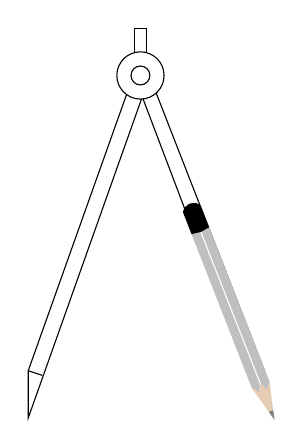
\begin{tikzpicture}
\begin{scope}[rotate=0,transform shape,scale=3]
\draw (2.95,3.7) rectangle (3,3.95);
\draw (2.92,3.68) -- (2.5,2.5) -- (2.5,2.3) -- (2.99,3.68);
\draw (3.5,2.5) -- (3.43,2.48) -- (2.975,3.68);
\draw (3.04,3.68) -- (3.5,2.5);
\draw (2.5,2.5) -- (2.56,2.48);
\draw[fill=white] (2.975,3.75) circle (0.1cm);
\draw (2.975,3.75) circle (0.04cm);
\end{scope}
\begin{scope}[xshift=10.34cm,yshift=7.28cm,rotate=21.4,scale=.6]          
\fill[gray!50] (0,4) -- (0.4,4) -- (0.4,0) --
               (0.3,-0.15) -- (0.2,0) -- (0.1,-0.14) --
               (0,0) -- cycle;
\draw[color=white] (0.2,4) -- (0.2,0);
\fill[black] (0,3.5) -- (0.2,3.47) -- (0.4,3.5) --
             (0.4,4) arc(30:150:0.23cm);
\fill[brown!40] (0,0) -- (0.2,-0.8)
    node[coordinate,pos=0.75](a){} -- 
    (0.4,0)node[coordinate,pos=0.25](b){} -- 
    (0.3,-0.15) -- (0.2,0) -- (0.1,-0.14) -- cycle;
\fill[gray] (a) -- (0.2,-0.8) -- (b) -- cycle;
\end{scope}
\end{tikzpicture}
\selectlanguage{hebrew}
\caption{מחוגה קבועה. לרגל אחת סיכה שניתן להניח במרכז המעגל. עפרון מחוברת לרגל השניה משמש לשרטוט המעגל. הרגלים מחוברות בציר קשיח כך שהמרחק בין הרגליים (רדיוס המעגל) נשמר גם כאשר מרימים את המחוגה מהנייר.}
\label{fig.fixed-compass}
\end{subfigure}
\hspace{3em}
\begin{subfigure}[b]{.4\textwidth}
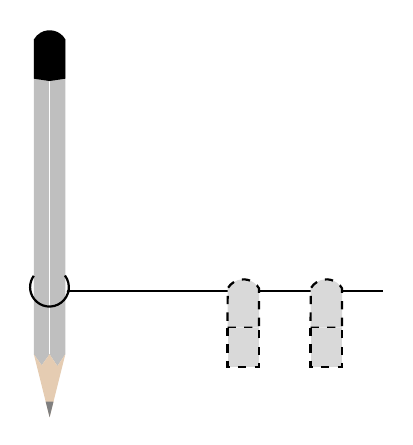
\begin{tikzpicture}[rotate=0,scale=1]          
\fill[gray!50] (0,4) -- (0.4,4) -- (0.4,0) --
               (0.3,-0.15) -- (0.2,0) -- (0.1,-0.14) --
               (0,0) -- cycle;
\draw[color=white] (0.2,4) -- (0.2,0);
\fill[black] (0,3.5) -- (0.2,3.47) -- (0.4,3.5) --
             (0.4,4) arc(30:150:0.23cm);
\fill[brown!40] (0,0) -- (0.2,-0.8)
    node[coordinate,pos=0.75](a){} -- 
    (0.4,0) node[coordinate,pos=0.25](b){} -- 
    (0.3,-0.15) -- (0.2,0) -- (0.1,-0.14) -- cycle;
\fill[gray] (a) -- (0.2,-0.8) -- (b) -- cycle;

\draw[thick] (0.395,1) arc (37:-216:7pt);
\coordinate (knot) at (0.44,.8);
\draw[thick] (knot) -- +(4,0);
\fill (knot) circle (.7pt);

\begin{scope}[xshift=100pt,yshift=-90pt]
\draw[dashed,thick,fill=white!70!gray] (0,3.5) -- (0.4,3.5) -- 
      (0.4,4) arc(30:150:0.23cm) -- cycle;
\draw[dashed,thick,fill=white!70!gray] (0,3.5) -- ++(0,-.5) -- ++(.4,0) -- ++(0,.5);
\end{scope}

\begin{scope}[xshift=70pt,yshift=-90pt]
\draw[dashed,thick,fill=white!70!gray] (0,3.5) -- (0.4,3.5) -- 
      (0.4,4) arc(30:150:0.23cm) -- cycle;
\draw[dashed,thick,fill=white!70!gray] (0,3.5) -- ++(0,-.5) -- ++(.4,0) -- ++(0,.5);
\end{scope}
\end{tikzpicture}
\selectlanguage{hebrew}
\caption{%
מחוגה מתמוטטת. המשתמש מצמיד חוט למרכז המעגל. לקצה השני של החוט מחובר עפרון המשמש לשרטוט המעגל. כאשר מרימים את המחוגה מהנייר, האצבעות (מקווקווים) יכולים בקלות להחליק למקום אחר.%
}\label{fig.collapsing-compass}
\end{subfigure}
\end{center}
\end{figure}

בתחילת הפרק דיון על הרלוונטית של למידה של בניה עם סרגל ומחוגה (סעיף%
~\ref{s.relevance}).
סעיף%
~\ref{s.collapse} 
משווה את שני סוגי המחוגה בבניה הפשוטה ביותר: אנח אמצעי. סעיף%
~\ref{s.collapse-copy}
מביא את השיטה של אוקלידס להעתקת קטע קו באמצעות מחוגה מתמוטטת. זה מוכיח שניתן לבצע באמצעות מחוגה מתמוטטת כל בניה שניתנת לביצוע באמצעות מחוגה קבועה. סעיף%
~\ref{s.collapse-copy-incorrect} 
מציג הוכחה של משפט זה שנראית נכונה אבל שלא עובדת עבור כל תצורה של קווים ונקודות. כדי להדגיש שאין לסמוך על שרטוט, סעיף%
~\ref{s.collapse-isoceles}
מביא "הוכחה לכאורה" מפורסמת ש-
\textbf{כל}
משולש הוא שווי שוקיים. ההוכחה נראית נכונה אבל היא שגויה כי היא מתבססת על שרטוט לא נכון.

%%%%%%%%%%%%%%%%%%%%%%%%%%%%%%%%%%%%%%%%%%%%%%%%%%%%%%%%%%%%%%%

\section{בניה עם סרגל ומחוגה}\label{s.relevance}

עד לאחרונה בנייה עם סרגל ומחוגה היתה המושג הבסיסי שנלמד בגיאומטריה אוקלידית, אולם חשיבותה ירדה בסילבוסים מודרניים. מובן שלנושא אין כמעט חשיבות מעשיות. כפי שאנו מראים בסעיפים%
~\ref{s.neusis}, \ref{s.neusis-doubling}, \ref{s.q}, \ref{s.square-quad},
היוונים ידעו לבנות בניות שאינן אפשריות עם סרגל ומחוגה באמצעות כליםי שהם רק מעט מתקדמים יותר. היום מחשבים מסוגלים לבצע בניות בדיוק רב כלל שנרצה באמצעות חישובים נומריים.

למרות זאת, אני מאמין שיש יתרונות ללמוד בניות עם סרגל ומחוגה:
\begin{itemize}
\item
מעניין יותר ומאתגר יותר ללמוד גיאומטריה דרך בניות לעומת קריאה של משפטים והוכחות.
\item
התקדמויות מכריעות במתמטיקה הושגו במסגרת נסיונות למצוא בניות. פרק%
~\ref{c.heptadecagon}
מביא בנייה של 
\L{Gauss}
שהיתה נקודת מוצא של אלגברה אבסטרקטית מודרנית, במיוחד התיאוריה שפותחה על יד 
\L{\'{E}variste Galois}.
\item
העובדה שיש בניות שאינן אפשריות קשה לעיכול ולכן מאוד מעניין.
\item
מעציב אבל אנשים רבים בעולם מבזבזים שנים של חייהם בניסיון לבצע בניות שאינן אפשריות. חשוב שתלמידים יכירו שהמאמצים הללו חסרי תוחלת.
\end{itemize}


%%%%%%%%%%%%%%%%%%%%%%%%%%%%%%%%%%%%%%%%%%%%%%%%%%%%%%%%%%%%%%%

\section{מחוגה קבועה ומחוגה מתמוטטת}\label{s.collapse}

$\overline{AB}$
שווה כמובן לאורך של
$\overline{BA}$,
ולכן למעגלים רדיוס זהה.

בבניה עם המחוגה המתמוטטת קל להוכיח שמתקבל משולש שווה-צלעות. האורך של
$\overline{AC}$
שווה לאורכו של
$\overline{AB}$,
כי שניהם רדיוסים של אותו מעגל, ומאותה סיבה האורך של
$\overline{BC}$
שווה לאורכו של
$\overline{BA}$.
מכאן ש-%
$\overline{AC} = \overline{AB} = \overline{BA} = \overline{BC}$.

הבניה של משולש שווה-צלעות היא המשפט הראשון בספר של אוקלידס. המשפט השני מראה שאפשר להעתיק קטע קו עם מחוגה מתמוטטת, ולכן המחוגה הקבועה לא מוסיפה יכולת חדשה. 

בספרי לימוד גיאומטריה ניתן למצוא בנייה של אנך אמצעי לקטע קו על ידי בניית שני מעגלים שמרכזם על הקו, 
\textbf{ובלבד שהרדיוס גדול ממחצית המרחק בין המרכזים},
)תרשים שמאלי(:

%%%%%%%%%%%%%%%%%%%%%%%%%%%%%%%%%%%%%%%%%%%%%%%%%%%%%%%%%%%%%%%


\section{העתקת קטע קו לפי אוקלידס}\label{s.collapse-copy}

\begin{theorem}
נתון קטע קו
$\overline{AB}$
ונקודה
$C$,
ניתן לבנות עם מחוגה מתמוטטת בנקודה
$C$
קטע קו שאורכו שווה לאורכו של 
$\overline{AB}$.
(איור%
~\ref{f.collapse-copying-1}).
\end{theorem}

\begin{figure}[htb]
\begin{center}
\begin{subfigure}{.4\textwidth}
\begin{tikzpicture}[scale=0.5]
\coordinate (A) at (0,0);
\coordinate (B) at (4,0);
\vertex{A};
\vertex{B};
\draw (A) node[below left] {$A$} -- (B) node[below right] {$B$};
\draw[name path=larc] (A) ++(-60:3cm) arc (-60:60:3cm);
\draw[name path=rarc] (B) ++(-120:3cm) arc (-120:-240:3cm);
\path [name intersections={of=larc and rarc,by={b,t}}];
\node[above right,xshift=-2pt,yshift=5pt] at (t) {$C$};
\node[below left,xshift=2pt,yshift=-5pt] at (b) {$D$};
\draw ($ (b) ! 1.2 ! (t)$) -- ($ (t) ! 1.2 ! (b)$);
\end{tikzpicture}
\selectlanguage{hebrew}
\caption{בניית חוצה אנכי עם מחוגה קבועי}\label{f.collapse-perp-bisector-fixed}
\end{subfigure}
\hfill
\begin{subfigure}{.4\textwidth}
\begin{tikzpicture}[scale=0.5]
\coordinate (A) at (0,0);
\coordinate (B) at (4,0);
\vertex{A};
\vertex{B};
\draw (A) node[below left] {$A$} -- (B) node[below right] {$B$};
\draw[name path=larc] (A) ++(-80:4cm) arc (-80:80:4cm);
\draw[name path=rarc] (B) ++(-100:4cm) arc (-100:-260:4cm);
\path [name intersections={of=larc and rarc,by={b,t}}];
\node[above right,xshift=-2pt,yshift=3pt] at (t) {$C$};
\node[below left,xshift=2pt,yshift=-3pt] at (b) {$D$};
\draw ($ (b) ! 1.2 ! (t)$) -- ($ (t) ! 1.2 ! (b)$);
\end{tikzpicture}
\selectlanguage{hebrew}
\caption{בניית חוצה אנכי עם מוחגה מתמוטטת}\label{f.collapse-perp-bisector-collapse}
\end{subfigure}
\end{center}
\end{figure}


\begin{figure}[htb]
\begin{center}
\begin{subfigure}{.4\textwidth}
\begin{tikzpicture}[scale=0.5]
\coordinate (A) at (0,0);
\coordinate (B) at (4,0);
\vertex{A};
\vertex{B};
\draw (A) node[below left] {$A$} -- (B) node[below right] {$B$};
\draw[name path=larc] (A) ++(-60:3cm) arc (-60:60:3cm);
\draw[name path=rarc] (B) ++(-120:3cm) arc (-120:-240:3cm);
\path [name intersections={of=larc and rarc,by={b,t}}];
\vertex{t};
\vertex{b};
\node[above right,xshift=-2pt,yshift=5pt] at (t) {$C$};
\node[below left,xshift=2pt,yshift=-5pt] at (b) {$D$};
\draw (A) -- (t);
\draw (B) -- (t);
\end{tikzpicture}
\selectlanguage{hebrew}
\caption{בניית משולש שווה-שוקיים עם מחוגה קבועה}\label{f.collapse-equilateral-fixed}
\end{subfigure}
\hspace{3em}
\begin{subfigure}{.4\textwidth}
\begin{tikzpicture}[scale=0.5]
\coordinate (A) at (0,0);
\coordinate (B) at (4,0);
\draw (A) node[below left] {$A$} -- (B) node[below right] {$B$};
\vertex{A};
\vertex{B};
\draw[name path=larc] (A) ++(-80:4cm) arc (-80:80:4cm);
\draw[name path=rarc] (B) ++(-100:4cm) arc (-100:-260:4cm);
\path [name intersections={of=larc and rarc,by={b,t}}];
\vertex{t};
\vertex{b};
\node[above right,xshift=-2pt,yshift=3pt] at (t) {$C$};
\node[below left,xshift=2pt,yshift=-3pt] at (b) {$D$};
\draw (A) -- (t);
\draw (B) -- (t);
\end{tikzpicture}
\selectlanguage{hebrew}
\caption{בניית משולש שווה-צלעות עם מחוגה מתמוטטת}\label{f.collapse-equilateral-collapse}
\end{subfigure}
\end{center}
\end{figure}

\begin{figure}[htb]
\begin{center}
\begin{subfigure}{.4\textwidth}
\begin{tikzpicture}[scale=0.5]
\coordinate (C) at (0,0);
\coordinate (A) at (3,0);
\draw (A) node[below,xshift=-2pt,yshift=-2pt] {$A$} -- +(40:4) coordinate (B) node[right] {$B$};
\vertex{A};
\vertex{B};
\vertex{C};
\node[below,xshift=2pt,yshift=-2pt] at (C) {$C$};
\draw[thick,dashed] (C) -- +(160:4) coordinate (D) node[below] {$C'$};
\vertex{D};
\end{tikzpicture}
\selectlanguage{hebrew}
\caption{העתקת קטע קו$\overline{AB}$; אין חשיבות לכיוון של $\overline{CC'}$}\label{f.collapse-copying-1}
\end{subfigure}
\hspace{3ex}
\begin{subfigure}{.4\textwidth}
\begin{tikzpicture}[scale=0.5]
\coordinate (C) at (0,0);
\coordinate (A) at (3,0);
\draw (A) node[below,xshift=-2pt,yshift=-2pt] {$A$} -- +(40:4) coordinate (B) node[right] {$B$};
\vertex{B};
\node[below,xshift=2pt,yshift=-2pt] at (C) {$C$};
\draw (A) -- (C);
\path[name path=larc] (C) ++(-70:2.5cm) arc (-70:70:2.5cm);
\path[name path=rarc] (A) ++(-110:2.5cm) arc (-110:-250:2.5cm);
\path [name intersections={of=larc and rarc,by={d,D}}];
\node[above] at (D) {$D$};
\draw (A) -- (D);
\draw (C) -- (D);
\end{tikzpicture}
\selectlanguage{hebrew}
\caption{העתקת קו עם מחוגה מתמוטטת}\label{f.collapse-copying-2}
\end{subfigure}
\end{center}
\end{figure}

\begin{proof}

\textbf{בניה:}
\begin{itemize}
\item
חברו בקו את הנקודות
$A$
ו-%
$C$.
\item
בנו משולש שווה צלעות שבסיסו
$\overline{AC}$
(איור%
~\ref{f.collapse-copying-2}).
סמנו את הקודקוד של המשולש ב-%
$D$
)תרשים ימני למעלה(. 
\item
בנו קרן בהמשך של
$\overline{DA}$
וקרן בהמשך של 
$DC$
(\ref{f.collapse-copying-3}).
\item
בנו מעגל שמרכזו 
$A$
עם רדיוס
$\overline{AB}$.
סמנו
$E$,
החיתוך של המעגל עם הקרן
$\overline{DE}$
(איור%
~\ref{f.collapse-copying-4}).

\begin{figure}[htb]
\begin{center}
\begin{subfigure}{.4\textwidth}
\begin{tikzpicture}[scale=0.6]
\coordinate (C) at (0,0);
\coordinate (A) at (2.5,0);
\coordinate (B) at (5.5,2);
\draw (A) node[below,xshift=-2pt,yshift=-2pt] {$A$} -- (B) node[right] {$B$};
\fill (A) circle[radius=3pt];
\fill (B) circle[radius=3pt];
\fill (C) node[below,xshift=2pt,yshift=-2pt] {$C$} circle[radius=3pt];
\draw (A) -- (C);
\path[name path=larc] (C) ++(-70:2.5cm) arc (-70:70:2.5cm);
\path[name path=rarc] (A) ++(-110:2.5cm) arc (-110:-250:2.5cm);
\path [name intersections={of=larc and rarc,by={d,D}}];
\fill (D) node[above] {$D$} circle[radius=3pt];
\draw (A) -- (D);
\draw (C) -- (D);
\draw[name path=ray2] (D) -- ($ (D) ! 2.7 ! (C) $);
\draw[name path=ray1] (D) -- ($ (D) ! 2.7 ! (A) $);
\end{tikzpicture}
\selectlanguage{hebrew}
\caption{בניית קרניים מ-%
$D$}\label{f.collapse-copying-3}
\end{subfigure}
\hspace{3ex}
\begin{subfigure}{.4\textwidth}
\begin{tikzpicture}
\coordinate (C) at (0,0);
\coordinate (A) at (2.5,0);
\coordinate (B) at (5.5,2);
\draw (A) node[below,xshift=-2pt,yshift=-2pt] {$A$} -- (B) node[right] {$B$};
\fill (A) circle[radius=3pt];
\fill (B) circle[radius=3pt];
\fill (C) node[below,xshift=2pt,yshift=-2pt] {$C$} circle[radius=3pt];
\draw (A) -- (C);
\path[name path=larc] (C) ++(-70:2.5cm) arc (-70:70:2.5cm);
\path[name path=rarc] (A) ++(-110:2.5cm) arc (-110:-250:2.5cm);
\path [name intersections={of=larc and rarc,by={d,D}}];
\fill (D) node[above] {$D$} circle[radius=3pt];
\draw (A) -- (D);
\draw (C) -- (D);
\draw[name path=ray2] (D) -- ($ (D) ! 2.7 ! (C) $);
\draw[name path=ray1] (D) -- ($ (D) ! 2.7 ! (A) $);
\node[draw,circle through=(B),name path=c1] at (A) {};
\path [name intersections={of=c1 and ray1,by={E,e}}];
\fill (E) node[right,xshift=2pt,yshift=-2pt] {$E$} circle[radius=3pt];
\end{tikzpicture}
\selectlanguage{hebrew}
\caption{בניית מעגל עם רדיוס 
$\overline{AB}$}\label{f.collapse-copying-4}
\end{subfigure}
\end{center}
\end{figure}
\item
בנו מעגל שמרכזו 
$D$
עם רדיוס 
$\overline{DE}$.
סמנו את החיתוך של
$\overline{DC}$
עם המעגל ב-%
$F$
(איור%
~\ref{f.collapse-copying-5}).
\end{itemize}

\begin{figure}[htb]
\begin{center}
\begin{tikzpicture}[scale=0.4]
\coordinate (C) at (0,0);
\coordinate (A) at (2.5,0);
\coordinate (B) at (5.5,2);
\draw (A) node[below,xshift=-2pt,yshift=-2pt] {$A$} -- node[above] {$x$} (B) node[right] {$B$};
\fill (A) circle[radius=3pt];
\fill (B) circle[radius=3pt];
\fill (C) node[below,xshift=2pt,yshift=-2pt] {$C$} circle[radius=3pt];
\draw (A) -- (C);
\path[name path=larc] (C) ++(-70:2.5cm) arc (-70:70:2.5cm);
\path[name path=rarc] (A) ++(-110:2.5cm) arc (-110:-250:2.5cm);
\path [name intersections={of=larc and rarc,by={d,D}}];
\fill (D) node[above] {$D$} circle[radius=3pt];
\draw (A) -- node[right] {$y$} (D);
\draw (C) -- node[left] {$y$} (D);
\draw[name path=ray2] (D) -- ($ (D) ! 3 ! (C) $);
\draw[name path=ray1] (D) -- ($ (D) ! 3 ! (A) $);
\node[draw,circle through=(B),name path=c1] at (A) {};
\path [name intersections={of=c1 and ray1,by={E,e}}];
\fill (E) node[right,xshift=2pt,yshift=-2pt] {$E$} circle[radius=3pt];
\node[draw,circle through=(E),name path=c2] at (D) {};
\path [name intersections={of=c2 and ray2,by={F,f}}];
\fill (F) node[left,xshift=-2pt,yshift=-2pt] {$F$} circle[radius=3pt];
\path (A) -- node[right] {$x$} (E);
\path (C) -- node[left] {$x$} (F);
\end{tikzpicture}
\selectlanguage{hebrew}
\caption{בניית $\overline{CF}=\overline{AB}$}\label{f.collapse-copying-5}
\end{center}
\end{figure}

\textbf{טענה:}
אורכו של קטע הקו
$\overline{CF}$
שווה לאורכו של קטע הקו
$\overline{AB}$.

\textbf{הוכחה:}
$\overline{DC}=\overline{DA}$
כי
$\triangle ACD$
שווה-צלעות.
$\overline{AE}=\overline{AB}$
כי שניהם רדיוסים של המעגל שמרכזו 
$A$.
$\overline{DF}=\overline{DE}$
כי שניהם רדיוסים של המעגל שמרכזו
$D$.
אורכו של
$\overline{CF}$ 
הוא:
\[
\overline{CF} = \overline{DF} - \overline{DC} = \overline{DE} - \overline{DC} = \overline{DE} - \overline{DA} = \overline{AE} = \overline{AB}\,.
\].
\end{proof}

%%%%%%%%%%%%%%%%%%%%%%%%%%%%%%%%%%%%%%%%%%%%%%%%%%%%%%%%%%%%%%%

\section{העתקה שגויה של קטע קו}\label{s.collapse-copy-incorrect}

\begin{itemize}
\item
בנו מעגל שמרכזו
$A$
עם רדיוס
$\overline{AB}$.
\begin{figure}[htb]
\begin{center}
\begin{tikzpicture}[scale=0.4]
\clip (-12,-6) rectangle (11,10);
\coordinate (C) at (-4,0);
\coordinate (A) at (3,0);
\draw (A) node[below,xshift=-2pt,yshift=-2pt] {$A$} -- +(40:4) coordinate (B) node[right] {$B$};
\node[below,xshift=2pt,yshift=-2pt] at (C) {$C$};
\draw (A) -- (C);
\path[name path=larc] (C) ++(-70:7cm) arc (-70:70:7cm);
\path[name path=rarc] (A) ++(-110:7cm) arc (-110:-250:7cm);
\path [name intersections={of=larc and rarc,by={d,D}}];
\node[above] at (D) {$D$};
\draw (A) -- (D);
\draw (C) -- (D);
\draw[name path=ray2] (D) -- ($ (D) ! 2 ! (C) $);
\draw[name path=ray1] (D) -- ($ (D) ! 2 ! (A) $);
\node[draw,circle through=(B),name path=c1] at (A) {};
\path [name intersections={of=c1 and ray1,by={e,E}}];
\node[right,xshift=2pt,yshift=-2pt] at (E) {$E$};
\node[draw,circle through=(E),name path=c2] at (D) {};
\path [name intersections={of=c2 and ray2,by={F,f}}];
\node[left,xshift=-2pt,yshift=-2pt] at (F) {$F$};
\path (A) -- node[right] {$a$} (E);
\path (C) -- node[left] {$a$} (F);
\draw[white,fill=white] (-12,8) rectangle +(23,2);
\end{tikzpicture}
\end{center}
\selectlanguage{hebrew}
\caption{בנייה עבור $\overline{AC}>\overline{AB}$}\label{f.collapse-copying-6}
\end{figure}
%\begin{figure}[htb]
%\begin{center}
%\begin{subfigure}{.4\textwidth}
%\begin{tikzpicture}[scale=0.6]
%\begin{scope}
%\coordinate (C) at (-2,0);
%\coordinate (A) at (2.5,0);
%\coordinate (B) at (4.5,1.5);
%\draw (A) node[below,xshift=-2pt,yshift=-2pt] {$A$} -- (B) node[right] {$B$};
%\fill (A) circle[radius=3pt];
%\fill (B) circle[radius=3pt];
%\fill (C) node[below,xshift=2pt,yshift=-2pt] {$C$} circle[radius=3pt];
%\end{tikzpicture}
%\caption{}\label{}
%\end{subfigure}
%\hspace{3ex}
%\begin{subfigure}{.4\textwidth}
%\begin{tikzpicture}
%\coordinate (C) at (-2,0);
%\coordinate (A) at (2.5,0);
%\coordinate (B) at (4.5,1.5);
%\draw (A) node[below,xshift=-2pt,yshift=-2pt] {$A$} -- (B) node[right] {$B$};
%\fill (A) circle[radius=3pt];
%\fill (B) circle[radius=3pt];
%\fill (C) node[below,xshift=2pt,yshift=-2pt] {$C$} circle[radius=3pt];
%\node[draw,circle through=(B),name path=c1] at (A) {};
%\end{tikzpicture}
%\caption{}\label{}
%\end{subfigure}
%\end{center}
%\end{figure}
%\vspace*{-8ex}
\item
בנו מעגל שמרכזו
$A$
עם רדיוס
$\overline{AC}$
ומעגל שמרכזו
$C$
עם רדיוס
$\overline{AC}=\overline{CA}$.
\item
סמנו את נקודות החיתוך של המעגלים ב-%
$E,F$.
סמנו את נקודת החיתוך של המעגל שמרכזו
$C$
עם המעגל שמרכזו 
$A$
עם רדיוס
$\overline{AB}$
ב-%
$D$.
אם
$\overline{AC}>\overline{AB}$,
הבנייה היא כפי שרואים באיור%
~\ref{f.collapse-incorrect-1}.
\begin{figure}[htb]
\begin{center}
\begin{tikzpicture}[scale=0.6]
\coordinate (C) at (-2,0);
\coordinate (A) at (2.5,0);
\coordinate (B) at (4.5,1.5);
\draw (A) node[below right] {$A$} -- (B) node[right] {$B$};
\fill (A) circle[radius=3pt];
\fill (B) circle[radius=3pt];
\fill (C) node[left,xshift=-2pt] {$C$} circle[radius=3pt];
\node[draw,circle through=(B),name path=c1] at (A) {};
\node[draw,circle through=(C),name path=c2] at (A) {};
\node[draw,circle through=(A),name path=c3] at (C) {};
\path [name intersections={of=c1 and c3,by={D,f}}];
\path [name intersections={of=c2 and c3,by={E,F}}];
\fill (D) node[below right,xshift=4pt] {$D$} circle[radius=3pt];
\fill (E) node[above,yshift=2pt] {$E$} circle[radius=3pt];
\fill (F) node[below,yshift=-2pt] {$F$} circle[radius=3pt];
\end{tikzpicture}
\selectlanguage{hebrew}
\end{center}
\caption{בניית עבור העתקת קו (1)}\label{f.collapse-incorrect-1}
\end{figure}
\item
בנו מעגל שמרכזו 
$E$
עם רדיוס 
$\overline{ED}$.
סמנו ב-%
$G$
את החיתוך של המעגל עם המעגל שמרכזו
$A$
עם רדיוס 
$\overline{AC}$
(איור~%
\ref{f.collapse-incorrect-2}).
\end{itemize}

\begin{figure}[htb]
\begin{center}
\begin{tikzpicture}[scale=0.5]
\clip (-8,-1) rectangle (9,5);
\coordinate (C) at (-2,0);
\coordinate (A) at (2.5,0);
\coordinate (B) at (4.5,1.5);
\draw[thick] (A) node[below right] {$A$} -- (B) node[right] {$B$};
\vertex{A};
\vertex{C};
\node[below left] at (C) {$C$};
\node[draw,circle through=(B),name path=c1] at (A) {};
\node[draw,circle through=(C),name path=c2] at (A) {};
\node[draw,circle through=(A),name path=c3] at (C) {};
\path [name intersections={of=c1 and c3,by={D,f}}];
\path [name intersections={of=c2 and c3,by={E,F}}];
\node[draw,circle through=(D),name path=c4] at (E) {};
\path [name intersections={of=c2 and c4,by={g,G}}];
\node[left] at (G) {$G$};
\node[below right,yshift=2pt,xshift=2pt] at (D) {$D$};
\node[above] at (E) {$E$};
\vertex{E};
\vertex{F};
\draw (C) -- (G);
\draw (A) -- (G) -- (E) -- (C) -- (D);
\draw (A) -- (D) -- (E) -- cycle;
\end{tikzpicture}
\end{center}
\selectlanguage{hebrew}
\caption{בניית עבור העתקת קו (2)}\label{f.collapse-incorrect-2}
\end{figure}


%\begin{figure}[htb][tb]
%\begin{center}

%\begin{tikzpicture}[scale=0.8]
%\clip (-8,-1) rectangle (9,5);
%\coordinate (C) at (-2,0);
%\coordinate (A) at (2.5,0);
%\coordinate (B) at (4.5,1.5);
%\draw[thick] (A) node[below right] {$A$} -- (B) node[right] {$B$};
%\fill (A) circle[radius=3pt];
%\fill (B) circle[radius=3pt];
%\fill (C) node[below left] {$C$} circle[radius=3pt];
%\node[draw,circle through=(B),name path=c1] at (A) {};
%\node[draw,circle through=(C),name path=c2] at (A) {};
%\node[draw,circle through=(A),name path=c3] at (C) {};
%\path [name intersections={of=c1 and c3,by={D,f}}];
%\path [name intersections={of=c2 and c3,by={E,F}}];
%\fill (D) node[below right,xshift=4pt] {$D$} circle[radius=3pt];
%\fill (E) node[above,yshift=2pt] {$E$} circle[radius=3pt];
%\fill (F) node[below,yshift=-2pt] {$F$} circle[radius=3pt];
%\node[draw,circle through=(D),name path=c4] at (E) {};
%\path [name intersections={of=c2 and c4,by={g,G}}];
%\fill (G) node[below left,xshift=-4pt] {$G$} circle[radius=3pt];
%\draw[thick] (C) -- (G);
%\draw[thick,dashed] (G) -- (E) -- (C);
%\draw[thick,dashed] (A) -- (D) -- (E) -- cycle;
%\end{tikzpicture}
%\end{center}
%\selectlanguage{hebrew}
%\caption{משולשים חופפים}\label{f.collapse1}
%\end{figure}

\textbf{טענה:}
ארכו של 
$\overline{CG}$
שווה לאורכו של
$\overline{AB}$.

\begin{proof}
נניח ש-%
$\triangle ADE\cong \triangle CGE$.
אם כן, 
$\overline{CG}=\overline{AD}=\overline{AB}$
כי 
$\overline{AD},\overline{AB}$
הם רדיוסים של המעגל הקטן שמרכזו 
$A$.
למעגל שמרכזו
$C$
אותו רדיוס כמו למעגל שמרכזו 
$A$
ועובר דרך 
$E$.
לכן, ניתן להתייחס אליהם כ-"אותו" מעגל.

עכשיו נוכיח את החפיפה
$\triangle ADE\cong \triangle CGE$.
$\overline{EG}=\overline{ED}$
כי הם רדיוסים של המעגל שמרכזו
$E$,
ו-%
$\overline{EC}=\overline{EA}$
כי הם רדיוסים של "אותו" מעגל. 
$\angle GCE=\angle DAE$
כי הן זוויות היקפיות על "אותו" מיתר 
$\overline{EG},\overline{ED}$.
 $\angle CGE=\angle ADE$
כי הן זוויות היקפיות על "אותו" מיתר
$\overline{EC},\overline{EA}$.
. לכן,
$\angle GEC=\angle DEA$
ו-%
$\triangle ADE\cong \triangle CGE$
לפי צ.ז.צ.
\end{proof}

אין שום שגיאה בהוכחה! השגיאה נובעת ממקור אחר: השווין
$\overline{AB}=\overline{GC}$
מתקיים רק כאשר אורכו של 
$\overline{AB}$
קטן מאורכו של
$\overline{AC}$.
הבנייה של אוקלידס נכונה ללא קשר לאורך היחסי של הקווים ולמיקום של הנקודה
$C$
ביחס לקטע הקו
$\overline{AB}$.

\begin{figure}[htb]
\begin{center}
\begin{tikzpicture}[scale=0.5]
\coordinate (C) at (-1,0);
\coordinate (A) at (2,0);
\coordinate (B) at (6,1.5);
\draw[thick] (A) node[below right] {$A$} -- (B) node[right] {$B$};
\node[left,xshift=-2pt] at (C) {$C$};
\node[draw,circle through=(B),name path=c1] at (A) {};
\node[draw,circle through=(C),name path=c2] at (A) {};
\node[draw,circle through=(A),name path=c3] at (C) {};
\path [name intersections={of=c1 and c3,by={D,f}}];
\path [name intersections={of=c2 and c3,by={E,F}}];
\node[above left,xshift=4pt] at (D) {$D$};
\node[above,yshift=2pt] at (E) {$E$};
\node[below,yshift=-2pt] at (F) {$F$};
\vertex{A};
\vertex{C};
\node[draw,circle through=(D),name path=c4] at (E) {};
\path [name intersections={of=c2 and c4,by={g,G}}];
\node[right,xshift=2pt,yshift=2pt] at (G) {$G$};
\draw[thick] (G) -- (C);
\end{tikzpicture}
\selectlanguage{hebrew}
\caption{תרשים עבורו ההוכחה לא עובדת}\label{f.collapse-incorrect-4}
\end{center}
\end{figure}

%%%%%%%%%%%%%%%%%%%%%%%%%%%%%%%%%%%%%%%%%%%%%%%%%%%%%%%%%%%%%%%

\section{
אין לסמוך על תרשים
}\label{s.collapse-isoceles}
בסעיף~%
\ref{s.collapse-copy-incorrect}
ראינו שאין לסמוך על ציור. הנה הוכחה "נכונה"
\textbf{\R{שכל}}
משולש שווה-שוקיים!

\begin{figure}[htb]
\begin{center}
\begin{tikzpicture}[scale=1.2]
\coordinate (P) at (0,0);
\node[xshift=4mm,yshift=1mm] at (P) {$P$};
\coordinate [label=left:$B$] (B)  at (-2,-2);
\coordinate [label=right:$C$] (C)  at (4,-2);
\coordinate [label=above:$A$] (A)  at (-1,2);
\node[below,yshift=-12pt,xshift=2pt] at (A) {$\alpha$};
\node[below,yshift=-12pt,xshift=15pt] at (A) {$\alpha$};
\draw (A) -- (B);
\draw (A) -- (C);
\draw (B) -- (C);
\draw (A) -- (P);
\draw (B) -- (P);
\draw (C) -- (P);
\coordinate[label=left:$E$] (E) at ($ (A) ! .44 ! (B) $);
\draw[rotate=-100] (E) rectangle +(8pt,8pt);
\draw (P) -- (E);
\coordinate[label=right:$F$] (F) at ($ (A) ! .33 ! (C) $);
\draw[rotate=-132] (F) rectangle +(8pt,8pt);
\draw (P) -- (F);
\coordinate[label=below:$D$] (D) at ($ (B) ! .33 ! (C) $);
\draw (D) rectangle +(8pt,8pt);
\draw (P) -- (D);
\node[left] at ($ (A) ! .5 ! (E) $) {};
\node[left] at ($ (B) ! .5 ! (E) $) {};
\node[below] at ($ (B) ! .5 ! (D) $) {$a$};
\node[below] at ($ (C) ! .5 ! (D) $) {$a$};
\node[right,xshift=2pt] at ($ (A) ! .5 ! (F) $) {};
\node[right,xshift=2pt] at ($ (C) ! .5 ! (F) $) {};
%\fill (A) circle(1pt);
%\fill (B) circle(1pt);
%\fill (C) circle(1pt);
\fill (D) circle(1pt);
\fill (E) circle(1pt);
\fill (F) circle(1pt);
\fill (P) circle(1pt);
\end{tikzpicture}
\selectlanguage{hebrew}
\caption{הוכחה שגוייה שכל משולש שווה-שוקיים}\label{f.isoceles}
\end{center}
\end{figure}

נתון משולש שרירותי 
$\triangle ABC$,
תהי
$P$
נקודת החיתוך בין חוצה הזווית של
$\angle BAC$
לבין האנך האמצעי של 
$\overline{BC}$
)איור
\ref{f.isoceles}(.
סמנו ב-%
$D,E,F$
את נקודות החיתוך של האנכים מ-%
$P$
לצלעות
$\overline{BC},\overline{AB},\overline{AC}$. $\triangle APE\cong \triangle APF$
כי הם משולשים ישר זווית עם זוויות שוות
$\alpha$
וצלע 
$\overline{AP}$
משותף.

$\triangle DPB\cong \triangle DPC$
לפי צ.ז.צ. כי 
$\overline{PD}$
הוא צלע משותף, 
$\angle PDB=\angle PDC=90^\circ$,
ו-%
$\overline{BD}=\overline{DC}=a$
כי 
$\overline{PD}$
הוא האנך האמצעי ל-%
$\overline{BC}$.
במשולשים ישר-זווית
$\triangle EPB\cong \triangle FPC$
כי שתי לצועות שוות:
$\overline{EP}=\overline{PF}$
לפי החפיפה הראשונה, ו-%
$\overline{PB}=\overline{PC}$
לפי החפיפה השנייה. נחבר את השוויונות ונקבל ש-%
$\triangle ABC$
שווה-שוקיים:
\[
\overline{AB}=\overline{AE}+\overline{EB}=\overline{AF}+\overline{FC}=\overline{AC}\,.
\]
\qed
הבעיה בהוכחה היא שתרשים אינו נכון כי הנקודה
$P$
נמצאת
\textbf{מחוץ}
למשולש כפי שניתן לראות מהציור המדוייק באיור%
~\ref{f.isoceles-wrong}.
\begin{figure}[htb]
\begin{center}
\begin{tikzpicture}[scale=.9]
\coordinate (B)  at (0,0);
\node[left] at (B) {$B$};
\coordinate (C)  at (7,0);
\node[right] at (C) {$C$};
\path[name path=pathb] (B) -- +(80:6.5);
\path[name path=pathc] (C) -- +(140:9.5);
\path [name intersections={of=pathb and pathc,by={A}}];
\node[above] at (A) {$A$};
%\fill (A) circle(1pt) node[above] {$A$};
%\fill (B) circle(1pt) node[left] {$B$};
%\fill (C) circle(1pt) node[right] {$C$};
\draw (A) -- (B) -- (C) -- cycle;
\draw[name path=angle] (A) -- +(-70:8.5);
\draw ($(B)!.5!(C)$) |- +(0,4);
\draw[name path=perp] ($(B)!.5!(C)$) |- +(0,-3);
\draw ($(B)!.5!(C)$) rectangle +(8pt,8pt);
\path [name intersections={of=angle and perp,by={P}}];
\fill (P) circle(3pt) node[right] {$P$};
\node[below,yshift=-12pt,xshift=2pt] at (A) {$\alpha$};
\node[below,yshift=-12pt,xshift=15pt] at (A) {$\alpha$};
\end{tikzpicture}
\selectlanguage{hebrew}
\caption{הסיבה שהבנייה לא עובדת}\label{f.isoceles-wrong}
\end{center}
\end{figure}

\subsection*{מה ההפתעה?}

כתלמיד היה לי ברור מאליו שלמחוגה ציר חיכוך ששומר את המרחק בין הוד והעפרון. הכאשר המורה השתשמשה במחוגה המורכבת מחוט וגיר, לא העליתי על דעתי שהיא שונה מהמחוגה שלי. המאמר של
\L{Gotfried Toussaint}
היה הפתעה גמורה, כמו גן ההצגה שלו שההוכחות שבאו לאחר 
\L{Euclid}
היו שגויות כי הן היו לתולויות בהנחות חסרות בסיס. אני ממליץ לקורא לעיין במאמר כדי להעמיק את הבנתם על הוכחות במתמטיקה.

\subsection*{מקורות}

הפרק מבוסס על
\cite{toussaint}.
ההוכחה השגויה בסעיף%
~\ref{s.collapse-copy-incorrect}
היא מ-%
\cite{rusty}.
תרגום שלם לאנגלית של ספר
\L{Elements}
של 
\L{Euclid}
ביחד עם פרשנות מפורטת נמצא ב-%
\cite{euclid}
שנכתב על ידי
\L{Thomas L. Heath}
שהיה אחד המומחים הבולטים למתמטיקה יוונית.



\tikzsetfigurename{trisect-an-angle}
% !TeX root = surprises.tex

\selectlanguage{hebrew}
\chapter{חלוקת זווית לשלושה חלקים}
\label{c.trisect}

%%%%%%%%%%%%%%%%%%%%%%%%%%%%%%%%%%%%%%%%%%%%%%%%%%%%%%%%%%%%%

לא ניתן לחלק זווית שרירותית לשלושה חלקים שווים באמצעות סרגל ומחוגה )להלן, בקיצור, לחלק זווית לשלושה(.
הסיבה היא שחלוקת זווית לשלושה דורשת בניה של שורש שלישי, אבל עם  וסרגל ומחוגה ניתן לבנות רק אורכים שמתקבלים מארבעת פעולות החשבון ושורש ריבועי.

היוונים גילו שבאמצעות כלים אחרים ניתן לחלק זווית לשלושה. סעיף~%
\ref{s.neusis}
מציג בניה של ארכימדס עם כלי פשוט הנקרא ביוונית ניאוסיס
\L{(neusis)}.
סעיף~%
\ref{s.q}
מביא בניה מסובכת יותר של היפיאס באמצעות
קוודרטריקס
\L{(quadratrix)}.
בסעיף~%
\ref{s.square}
נסביר איך לרבע מעגל באמצעות קוודרטריקס.


%%%%%%%%%%%%%%%%%%%%%%%%%%%%%%%%%%%%%%%%%%%%%%%%%%%%%%%%%%%%%

\section{חלוקת זווית לשלושה באמצעות ניאוסיס}\label{s.neusis}

השימוש במילה "סרגל" מטעה, כי הכוונה היא למקל ישר ללא כל סימן, שהפעולה היחידה שניתן לעשות איתו היא למתוח קו ישר בין שתי נקודות. לסרגל המוכר יש סימנים המאפשרים למדוד אורכים. כדי לחלק זווית לשלושה חלקים, נשתמש ב-%
\textbf{ניאוסיס}
שהוא מקל עם שני סימנים בלבד. נניח שהמרחק בין שני הסימנים הוא
$1$:
\begin{center}
\selectlanguage{english}
\begin{tikzpicture}[scale=3.5]
\draw (-1,1.05) rectangle +(3.2,.1);
\draw[thick] (1.89,1.05) -- +(0,.1);
\draw[thick] (.73,1.05) -- +(0,.1);
\draw[<->] (.73,1.25) -- node[fill=white] {$1$} (1.89,1.25);
\end{tikzpicture}
\end{center}
תהי 
$\alpha$
זווית שרירותית
$\angle ABE$
בתוך מעגל שמרכזו
$B$
עם רדיוס
$1$.
ניתן לבנות את המעגל על ידי קביעת המרחק שבין רגלי החוגה למרחק שבין הסימנים על הניאוסיס:
%\begin{figure}[H]
\begin{center}
\selectlanguage{english}
\begin{tikzpicture}[scale=2.5]
\coordinate (origin) at (0,0) node[below] {$B$} ;
\draw[name path=circle] (origin) circle [radius=1];
\draw (origin) node[above left,xshift=-4pt] {$\alpha$} -- (120:1) coordinate (a) node[below,xshift=-2pt] {$A$} ;
\draw (-1,0) -- (2.2,0);
\path[name path=ad] (a) -- (0,0 -| 2,0) coordinate (d) node[below] {$D$} ;
\path[name intersections={of=circle and ad,by={c,a1}}];
\fill (origin) circle [radius=.5pt];
\fill (a) circle [radius=.5pt];
\fill (c) circle [radius=.5pt] node [below,xshift=-4pt] {$C$};
\fill (d) circle [radius=.5pt];
\fill (-1,0) circle [radius=.5pt] node [left] {$E$};
\begin{scope}[rotate=-19,yshift=-11.25pt]
\draw (-1,1.05) rectangle +(3.2,.1);
\draw[thick] (1.89,1.05) -- +(0,.1);
\draw[thick] (.76,1.05) -- +(0,.1);
\draw[<->] (.73,1.25) -- node[fill=white] {$1$} (1.89,1.25);
\end{scope}
\end{tikzpicture}
\end{center}
%\caption{מיקום הניאוסיס יחסית למעגל היחידה}\label{f.neusis}
%\end{figure}

בנו קרן כהמשכו של 
$\overline{EB}$
מחוץ למעגל. הניחו את הניאוסיס על הנקודה
$A$
והזיזו אותו עד שהוא חותך את הקרן בנקודה 
$D$
ואת המעגל בנקודה
$C$.
כוונו את הניאוסיס כך שהאורך של
$\overline{CD}$
יהיה
$1$.
ציירו את הקו
$\overline{AD}$.
ציירו את הקו 
$\overline{BC}$
וסמנו את הזוויות וקטעי הקו לפי האיור להלן:
%\begin{figure}[bt]
\begin{center}
\selectlanguage{english}
\begin{tikzpicture}[scale=2.5]
\coordinate (origin) at (0,0) node[below] {$B$} ;
\draw[name path=circle] (origin) circle [radius=1];
\draw (origin) node[above left,xshift=-4pt] {$\alpha$} node[above,xshift=4pt,yshift=2pt] {$\delta$} node[above right,xshift=44pt,yshift=-2pt] {$\beta$} -- node[fill=white] {$1$} (120:1) coordinate (a) node[above left] {$A$} ;
\draw (-1,0) -- (2.2,0);
\draw[name path=ad] (a) node[below right,xshift=8pt,yshift=-6pt] {$\gamma$} -- (0,0 -| 2,0) coordinate (d) node[left,xshift=-50pt,yshift=7pt] {$\beta$} node[above right] {$D$} ;
\path[name intersections={of=circle and ad,by={c,a1}}];
\draw (origin) -- node[fill=white] {$1$}(c) node[above right] {$C$} node[left,xshift=-12pt] {$\gamma$} node[below,xshift=-2pt,yshift=-2pt] {$\epsilon$};
\fill (origin) circle [radius=.5pt];
\fill (a) circle [radius=.5pt];
\fill (d) circle [radius=.5pt];
\fill (c) circle [radius=.5pt];
\fill (-1,0) circle [radius=.5pt];
\path (c) -- node[fill=white] {$1$} (d);
\end{tikzpicture}
\end{center}
%\caption{חלוקת זווית לשלושה חלקים באמצעות ניאוסיס}%\label{f.trisection}
%\end{figure}
$\overline{BA}=\overline{BC}$
כי שניהם רדיוסים ו-%
$\overline{CB}=\overline{CD}$
לפי הבניה באמצעות הניאוסיס. לכן 
$\triangle ABC$, $\triangle BCD$
הם משולשים שווי-שוקיים. מחישוב פשוט:
\begin{equationarray*}{rcl}
\epsilon &=& 180^\circ - 2\beta\\
\gamma &=& 180^\circ - \epsilon = 2\beta\\
\delta &=& 180^\circ - 2\gamma = 180^\circ - 4\beta\\
\alpha &=& 180^\circ - \delta - \beta = 4\beta -\beta =3\beta\,,
\end{equationarray*}
מתקבל שהזווית
$\beta$
היא שליש מהזווית
$\alpha$.

%%%%%%%%%%%%%%%%%%%%%%%%%%%%%%%%%%%%%%%%%%%%%%%%%%%%%%%%%%%%%


\section{חלוקת זווית לשלושה באמצעות
קוודרטריקס%
}\label{s.q}

איור
\ref{f.quad}
מראה
\textbf{מחוגת קוודרטריקס}
המורכב משני סרגלים )ללא סימנים( המחוברים במפרק המאלץ אותם לנוע ביחד. סרגל אחד נע במקביל לציר ה-%
$x$
מ-%
$\overline{DC}$
עד
$\overline{AB}$.
הסרגל השני מחובר לנקודה
$A$
ומסתובב ממצב אנכי לאורך 
$\overline{AD}$
עד שהוא במצב אופקי לאורך 
$\overline{AB}$. 
העקומה המצוירת על ידי המפרק המחבר את שני הסרגלים נקראת
\textbf{עקומת הקוודרטריקס}
או פשוט
\textbf{קוודרטריקס}.
\begin{figure}[bt]
\begin{center}
\selectlanguage{english}
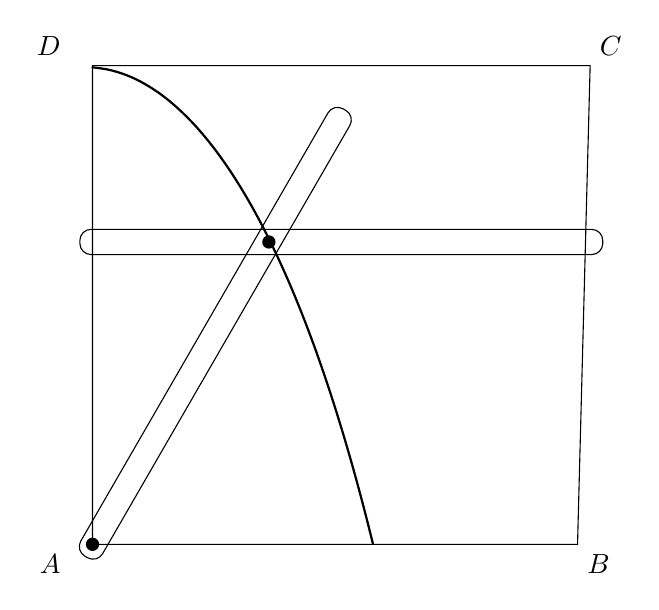
\begin{tikzpicture}[scale=.8,domain=.03:1.555,samples=100]
\draw (.1,.2) node[below left,xshift=-8pt] {$A$} -- (7.8,.2) node[below right] {$B$} -- (8,7.8) node[above right] {$C$} -- (.1,7.8) node[above left,xshift=-8pt] {$D$} -- cycle;
%\draw (.1,7.8) -- (.1,.2) -- (8,.1) -- (8,7.8);
\draw[rounded corners,rotate=60] (0,-.2) rectangle (8.2,.2);
\draw[rounded corners] (-.1,4.8) rectangle (8.2,5.2);
\fill (2.9,5) circle [radius=3pt];
\fill (.1,.2) circle [radius=3pt];
\draw[thick] plot (4.6*.637*\x,{12.2*.637*\x*cot(\x r)});
\end{tikzpicture}
\end{center}
\caption{קוודרטריקס}\label{f.quad}
\end{figure}

כאשר מזיזים את הסרגל האופקי במהירות אחידה, החיבור מאלץ את הסרגל השני להסתובב במהירות זוותית קבועה. למעשה זו ההגדרה של הקוודרטריקס.
כאשר קואורדינטת ה-%
$y$
של הסרגל האופקי יורד מ-%
$1$
ל-%
$0$,
הזווית של הסרגל השני יחסית לציר ה-%
$x$
יורד מ-%
$90^\circ$
ל-%
$0^\circ$.

איור~%
\ref{f.quad-trisection}
מראה איך לחלוק את הזווית 
$\alpha$
לשלושה חלקים באמצעות קוודרטריקס.
$P_1$
היא נקודת החיתוך בין הקו המגדיר את הזווית 
$\alpha$
לבין עקומת הקוודרטריקס.
קואורדינטת ה-%
$y$
שלה היא
$1-t$,
כאשר 
$t$
הוא המרחק שהסרגל האופקי נע מ-%
$\overline{DC}$.
חלקו את
$\overline{DE}$
לשלושה חלקים כדי לקבל את הנקודה
$F$.
$P_2$
היא נקודת החיתוך בין הקו מ-%
$F$
המקביל ל-%
$\overline{DC}$
לבין הקוודרטריקס.
לפי מהירויות שוות:
\erh{8pt}
\begin{equationarray*}{rcl}
\frac{\theta}{\alpha} &=& \frac{t/3}{t}\\
\theta &=& \alpha/3\,.
\end{equationarray*}

\begin{figure}[bth]
\begin{center}
\selectlanguage{english}
\begin{tikzpicture}[scale=.8,domain=.03:1.562,samples=100]
\draw (.1,7.8) coordinate (start) node[above left] {$D$} node[below right,xshift=32pt] {$\theta$} -- (.1,.2) node[below left] {$A$} -- (8,.1) node[below right] {$B$} -- (8,7.8) node[above right] {$C$} -- cycle;
\draw[name path=curve,thick] plot (4.6*.637*\x,{12.2*.637*\x*cot(\x r)});
\path[name path=twenty] (start) -- +(-35:9);
\path[name path=sixty] (start) -- +(-50:9);
\path[name path=xaxis] (.1,.2) -- (8,.1);
\path[name intersections={of=twenty and curve,by={x1,tri}}];
\draw (start) -- (tri);
\fill (tri) circle [radius=2pt] node[right] {$P_2$};
\path[name intersections={of=sixty and curve,by={x2,angle}}];
\fill (angle) circle [radius=2pt] node[right] {$P_1$};
\draw (start) -- (angle);
\path[name intersections={of=xaxis and curve,by=x}];
\fill (x) circle [radius=2pt];
%\path (.1,.2) -- node[below] {$2/\pi$} (x);
\draw[dashed] (tri) -- (tri -| .1,.2) coordinate (t3);
\fill (t3) circle [radius=2pt] node[left] {$F$};
\draw[dashed] (angle) -- (angle -| .1,.2) coordinate (t);
\fill (t) circle [radius=2pt] node[left] {$E$};
\draw[<->] (-1.2,7.8) -- node[fill=white] {$t/3$} (-1.2,7.8 |- t3);
\draw[<->] (-.6,7.8) -- node[fill=white] {$t$} (-.6,7.8 |- t);
\draw[<->] (-.6,7.8 |- t) -- node[fill=white] {$1-t$} (-.6,.2);
\draw (3.5,7.8) arc[start angle=0,delta angle=-49,radius=3.5];
\draw (1,7.8) arc[start angle=0,delta angle=-32,radius=1];
\node at (3.3,6) {$\alpha$}; 
\end{tikzpicture}
\end{center}
\caption{חלוקת זווית לשלושה באמצעות קוודרטריקס}\label{f.quad-trisection}
\end{figure}

%%%%%%%%%%%%%%%%%%%%%%%%%%%%%%%%%%%%%%%%%%%%%%%%%%%%%%%%%%%%%

\section{ריבוע מעגל באמצעות
קוודרטריקס%
}\label{s.square}

ניתן לרבע מעגל האמצעות קוודרטריקס )איור
\ref{f.quad-square}(.
\begin{figure}[tb]
\begin{center}
\selectlanguage{english}
\begin{tikzpicture}[scale=.8,domain=.01:1.57,samples=100]
\draw (0,0) node[below left] {$A$} node [above right,xshift=10pt] {$\theta$} -- (8,0) node[below right] {$B$} -- (8,8) node[above right] {$C$} -- (0,8) node[above left] {$D$} -- cycle;
\draw[name path=horiz] (0,5) -- (8,5);
\draw[name path=slant] (0,0) -- (61:8);
\path[name intersections={of=horiz and slant,by=joint}];
\draw[dashed] (joint) -- node[right] {$y$} (joint |- 0,0) coordinate (f);
\path (0,0) -- node[below] {$x$} (0,0 -| joint) node[below] {$F$};
\path (0,5) node[left] {$E$} -- node[left] {$t$} (0,8);
\path (0,0) -- node[left] {$1-t$} (0,5);
\fill (joint) circle [radius=2pt] node[above right,xshift=4pt] {$P$};
\fill (f) circle [radius=2pt];
\fill (0,5) circle [radius=2pt];
\fill (4.28,0) circle [radius=2pt] node[below] {$G$};
\draw[name path=curve,thick] plot (4.3*.637*\x,{12.5*.637*\x*cot(\x r)});
\end{tikzpicture}
\end{center}
\caption{ריבוע המעגל באמצעות קוודרטריקס}\label{f.quad-square}
\end{figure}
נניח שהסרגל האופקי נע מרחק 
$t$
לאורך ציר ה-%
$y$
עד לנקודה
$E$,
ושהסרגל המסתובב מגדיר זווית 
$\theta$
עם ציר ה-%
$x$.
הנקודה 
$P$
היא החיתוך בין הקוודרטריקס לבין הסרגל האופקי, והנקודה
$F$
היא היטל של 
$P$
על ציר ה-%
$x$.
מהן הקואורדינטות של הנקודה 
$P$?
ברור ש:
\[
y=\overline{PF}=\overline{EA}=1-t\,.
\]
על העקומה,
$\theta$
יורד באותו קצב ש-%
$t$
עולה:
\erh{12pt}
\begin{equationarray*}{rcl}
\disfrac{1-t}{1} &=& \disfrac{\theta}{\pi/2}\\
\theta &=&\disfrac{\pi}{2}(1-t)\,.
\end{equationarray*}
נבדוק אם זה הגיוני: כאשר
$t\!=\!0$
אז
$\theta\!=\!\pi/2$,
וכאשר
$t\!=\!1$
אז
$\theta\!=\!0$.
את קואורדינטת ה-%
$x$
של
$P$
נקבל בטריגונומטריה:
\[
\tan \theta = \frac{y}{x}\,.
\]
ומכאן:
\[
x = \frac{y}{\tan\theta}=y\cot\theta=y\cot \frac{\pi}{2}(1-t)=y\cot \frac{\pi}{2}y\,.
\]
בדרך כלל המשוואה של עקומה היא מהצורה
$y=f(x)$,
אבל אפשר גם להשתמש במשוואה מהצורה
$x=f(y)$.
נחשב את קוארדינטת ה-%
$x$
של הנקודה 
$G$,
החיתוך של ה%
קוודרטריקס
עם ציר ה-%
$x$.
לא ניתן להציב
$y=0$
כי
$\cot 0$
לא מוגדר, אבל ייתכן שיהיה לנו מזל אם נחשב את הגבול של
$x$
כאשר 
$y$
שואף ל-%
$0$:
\[
x = y\cot \frac{\pi}{2}y = \frac{2}{\pi}\cdot \frac{\pi}{2}y\cot \frac{\pi}{2}y\,.
\]
למען הנוחיות, נחליף משתנה
$z=\disfrac{\pi}{2}y$,
ואז נחשב את הגבול:
\[
\lim_{z\rightarrow 0} z\cot z = \lim_{z\rightarrow 0} \frac{z\cos z}{\sin z} = \lim_{z\rightarrow 0} \frac{\cos z}{\disfrac{\sin z}{z}} = \frac{\cos 0}{1} = 1\,,
\]
השתמשנו בעובדה הידועה ש-%
$\lim_{z\rightarrow 0} \disfrac{\sin z}{z}=1$.

כאשר
$y\rightarrow 0$:
\[
x \rightarrow \frac{2}{\pi}\cdot \lim_{y\rightarrow 0}\frac{\pi}{2}y\cot \frac{\pi}{2}y = \frac{2}{\pi}\cdot 1 = \frac{2}{\pi}\,.
\]
על ידי שימוש בקוודרטריקס בנינו קטע קו
$\overline{AG}$
שאורכו
$x=\disfrac{2}{\pi}$.
עם סרגל רגיל ומחוגה, קל לבנות קו באורך
$\sqrt{\pi}=\sqrt{\disfrac{2}{x}}$,
ואז לבנות ריבוע ששטחו
$\pi$.

\subsection*{מקורות}


על חלוקת זווית לשלושה חלקים ראו~%
\L{\cite{angle-trisection}}.
תיאור של הנאוסיס נמצא ב-%
\L{\cite{neusis-construction}}
ותיאור של הקוודרטריקס נמצא ב-%
\L{\cite{quadratrix}}.


\tikzsetfigurename{square-a-circle}
% !TeX root = surprises.tex

\selectlanguage{hebrew}
\chapter{איך לרבע את המעגל}
\label{c.square}


\section{
קירובים ל-%
$\pi$}\label{s.square-intro}

כדי לרבע מעגל יש לבנות את האורך 
$\sqrt{\pi}$,
אבל
$\pi$
הוא טרנסנדנטי, כלומר, הוא אינו פתרון של אף משוואה אלגברית. 
פרק זה מביא שלוש בניות של קירובים ל-%
$\pi$.
הטבלה שלהלן מביא את הנוסחאות של האורכים שנבנה, ערכם המספרי, ההפרש בין ערכים הללו והערך של 
$\pi$,
והשגיאה )במטרים( אם משתמשים בקירוב כדי לחשב את היקף כדור הארץ, כאשר נתון שהרדיוס הוא
$6378$
ק"מ.
\[
\selectlanguage{english}
%\renewcommand{\arraystretch}{1.2}
\begin{array}{|l|c|c|c|c|}
\hline
\textrm{\R{הבנייה}} & \textrm{\R{הנוסחה}} &\textrm{\R{הערך}} & \textrm{\R{ההפרש}} & \textrm{\R{השגיאה )מ(}}\\\hline
\pi & \textrm{\rule[-15pt]{0pt}{25pt}}& 3.14159265359 & - & -\\\hline
\textrm{Kochansky} & \textrm{\rule[-15pt]{0pt}{35pt}}\sqrt{\disfrac{40}{3}-2\sqrt{3}}&
  3.14153338705 & 5.932 \times 10^{-5} & 756\\\hline
\textrm{Ramanujan}\; 1 & \textrm{\rule[-15pt]{0pt}{35pt}}\disfrac{355}{113} &
  3.14159292035 &2.667  \times 10^{-7}&3.4\\\hline
\textrm{Ramanujan}\; 2 &\textrm{\rule[-15pt]{0pt}{35pt}}\left(9^2+\disfrac{19^2}{22}\right)^{1/4}&
  3.14159265258 & 1.007 \times 10^{-9}& 0.013\\\hline
\end{array}
\]
בבניות בפרק זה נצטרך לחלק
\textbf{קטע קו}
לשלושה חלקים. ניתן לבנות קטע קו בכל אורך רציונלי. נתון קטע קו באורך 
$1$
וקטעי קו באורכים 
$a,b$,
לפי משולשים דומים
$1/b=\overline{OD}/a$
ולכן
$\overline{OD}=a/b$.
%\begin{figure}[H]
\begin{center}
\selectlanguage{english}
\begin{tikzpicture}
%\clip (-.6,-1) rectangle (4,3);
\draw[name path=horz] (0,0) coordinate (o) -- (7,0);
\fill (o) circle(1.5pt) node[left] {$O$};
\fill (6,0) circle(1.5pt) coordinate (a) node[below] {$A$};
\draw (0,0) -- (30:5.5);
\fill (30:3) circle(1.5pt) coordinate (c) node[above] {$C$};
\fill (30:5) circle(1.5pt) coordinate (b) node[above] {$B$};
\draw (a) -- (b);
\path[name path=par] (c) -- +($(a)-(b)$);
\path[name intersections={of=par and horz,by=d}];
\fill (d) circle(1.5pt) node[below] {$D$};
\draw (c) -- (d);
\draw[<->] (-.4,.5) -- node[fill=white] {$b$} +(30:5.2);
\path (o) -- node[above] {$1$} (c);
\draw[<->] (0,-.8) -- node[fill=white] {$a$} +(6,0);
\path (o) -- node[below] {$a/b$} (d);
\end{tikzpicture}
\end{center}
%\caption{חילוק במשולשים דומים}\label{f.similar}
%\end{figure}

\newpage


%%%%%%%%%%%%%%%%%%%%%%%%%%%%%%%%%%%%%%%%%%%%%%%%%%%%%%%%%%%%%%%

\section{הבניה של
\L{Kochansky}}

\begin{itemize}
\item
בנו מעגל יחידה שמרכזו 
$O$,
עם קוטר
$\overline{AB}$
ובנו משיק למעגל ב-%
$A$.
\item
בנו מעגל יחידה שמרכזו
$A$.
סמנו את החיתוך עם המעגל הראשון ב-%
$C$.\footnote{%
עבור המעגל השני והשלישי, האיור מראה רק את הקשת החותך את המעגל הקודם.%
}
\item
בנו מעגל יחידה שמרכזו 
$C$.
סמנו את החיתוך שלו עם המעגל השני ב-%
$D$. 
\item
בנו
$\overline{OD}$
וסמנו את החיתוך שלו עם המשיק ב-%
$E$.
\item
מ-%
$E$
בנו
$F,G,H$,
כל אחת במרחק 
$1$
מהנקודה הקודמת, כך ש-%
$\overline{AH}=3-\overline{EA}$.
\item
בנו
$\overline{BH}$.
\end{itemize}
%\begin{figure}[bt]
\begin{center}
\selectlanguage{english}
\begin{tikzpicture}[scale=.5]
% Scale at 4

% Coordinates of circle
\coordinate (O) at (0,0);
\coordinate (A) at (0,-4);
\coordinate (B) at (0,4);
\fill (O) circle(2pt) node[above right] {$O$};
\fill (A) circle(2pt) node[below right] {$A$};
\fill (B) circle(2pt) node[above right] {$B$};
\draw (A) rectangle +(12pt,12pt);

% Draw circle and diameter
\node [thick,draw,circle through=(A),name path=circle] at (O) {};
\draw [thick] (A) -- (B);

% Draw tangent at A
\draw[thick,name path=tangent] ($(A)+(-4.5,0)$) -- ($(A)+(10.5,0)$);

% Draw arc centered at A which intersects circle at C
\draw[thick,name path=Aarc] (O)
   arc [start angle=90,end angle=220,radius=4];
\path[name intersections={of=circle and Aarc,by=C}];
\fill (C) circle(2pt) node[left,xshift=-4pt] {$C$};

% Draw arc centered at C which intersects the first arc at D
\draw[thick,name path=Carc] ($(C)+(260:4)$)
   arc [start angle=260,end angle=280,radius=4];
\path[name intersections={of=Carc and Aarc,by=D}];
\fill (D) circle(2pt) node[below left] {$D$};

% Draw O--D which intersects the tangent at E
\draw[thick,name path=OD] (O) -- (D);
\path[name intersections={of=tangent and OD,by=E}];
\fill (E) circle(2pt) node[above left] {$E$};

% Find point H at length 3 from E
\coordinate (F) at ($(E)+(4,0)$);
\fill (F) circle(2pt) node[above right,xshift=4pt] {$F$};
\coordinate (G) at ($(F)+(4,0)$);
\fill (G) circle(2pt) node[above] {$G$};
\coordinate (H) at ($(G)+(4,0)$);
\fill (H) circle(2pt) node[above] {$H$};

% Draw BH of length approximately pi
\draw[thick] (B) -- (H);
\end{tikzpicture}
\end{center}
%\caption{הבניה של \L{Kochansky}}\label{f.kochansky}
%\end{figure}

\textbf{טענה:}
$\overline{BH}=\sqrt{\disfrac{40}{3}-2\sqrt{3}}\approx \pi$.

\textbf{הוכחה:}
איור~%
\ref{f.kochansky}
מתמקד בחלק מהאיור למעלה. קטעי הקו המקווקווים נוספו. מפני שכל המעגלים הם מעגלי היחידה, קל לראות שאורך כל אחד מהקטעים המקווקווים הוא 
$1$.
מכאן ש-%
$AOCD$
הוא מעויין, ולכן האלכסונים שלו ניצבים זה לזה וחוצים זה את זה ב-%
$K$,
כך ש-%
$\overline{AK}=\frac{1}{2}$.
\begin{figure}
\begin{center}
\selectlanguage{english}
\begin{tikzpicture}[scale=1.2]
% Scale at 4

\clip (-4.5,-6.5) rectangle +(5,7);
% Coordinates of circle
\coordinate (O) at (0,0);
\coordinate (A) at (0,-4);
\coordinate (B) at (0,4);

% Draw circle
\node [circle through=(A),name path=circle] at (O) {};
\draw ($(O)+(200:4)$) arc [start angle=200,end angle=280,radius=4];

% Draw tangent at A
\draw[thick,name path=tangent] ($(A)+(-4.5,0)$) -- ($(A)+(10.5,0)$);
\draw (A) rectangle +(6pt,6pt);

% Draw arc centered at O which intersects circle at C
\draw[thin,name path=Aarc] (O)
   arc [start angle=90,end angle=220,radius=4];
\path[name intersections={of=circle and Aarc,by=C}];

% Draw arc centered at C which intersects the first arc at D
\draw[thin,name path=Carc] ($(C)+(260:4)$)
   arc [start angle=260,end angle=280,radius=4];
\path[name intersections={of=Carc and Aarc,by=D}];

% Draw O--D which intersects the tangent at E
\draw[thick,name path=OD] (O) -- (D);
\path[name intersections={of=tangent and OD,by=E}];

% Find point H at length 3 from E
\coordinate (F) at ($(E)+(4,0)$);
\coordinate (G) at ($(F)+(4,0)$);
\coordinate (H) at ($(G)+(4,0)$);

% Draw BH of length approximately pi
\draw[thick] (B) -- (H);

\draw[ultra thick,dashed] (A) -- (O) -- (C) -- (D) -- cycle;
\draw[ultra thick,dashed,name path=AC] (A) -- (C);

\node[above left,yshift=10pt,xshift=2pt] at (A) {$60^\circ$};
\node[left,yshift=10pt,xshift=-20pt] at (A) {$30^\circ$};

\path[name intersections={of=AC and OD,by=K}];
\draw[thick,rotate=-30] (K) rectangle +(6pt,6pt);

\path (A) -- node[above,xshift=2pt,yshift=2pt] {$1/2$} (K);
\path (A) -- node[below,xshift=-4pt] {$1/\sqrt{3}$} (E);

\fill (O) circle(1.25pt) node[above right] {$O$};
\fill (A) circle(1.25pt) node[below right] {$A$};
\fill (B) circle(1.25pt) node[above right] {$B$};
\fill (C) circle(1.25pt) node[left,xshift=-4pt] {$C$};
\fill (D) circle(1.25pt) node[below left] {$D$};
\fill (E) circle(1.25pt) node[above left] {$E$};
\fill (F) circle(1.25pt) node[above right,xshift=4pt] {$F$};
\fill (G) circle(1.25pt) node[above] {$G$};
\fill (H) circle(1.25pt) node[above] {$H$};
\fill (K) circle(1.25pt) node[above,yshift=4pt] {$K$};
\end{tikzpicture}
\end{center}
\caption{הוכחת הבניה של \L{Kochansky}}\label{f.kochansky}
\end{figure}

האלכסון
$\overline{AC}$
מייצר משולשים שווי-צלעות
$\triangle OAC, \triangle DAC$
כך ש-%
$\angle OAC=60^\circ$.
הזווית בין המשיק לרדיוס
$\overline{OA}$
היא זווית ישרה ולכן
$\angle KAE=30^\circ$.
נחשב:
\erh{12pt}
\begin{equationarray*}{rcl}
\disfrac{1/2}{\overline{EA}}&=&
\cos 30^\circ=\disfrac{\sqrt{3}}{2}\\
\overline{EA}&=&\disfrac{1}{\sqrt{3}}\\
\overline{AH}&=&3-\overline{EA}\\
&=&\left(3-\disfrac{1}{\sqrt{3}}\right)
=\disfrac{3\sqrt{3}-1}{\sqrt{3}}
\end{equationarray*}
נחזור לאיור הראשון.
$\triangle ABH$
הוא משולש ישר-זווית, ולפי משפט פיתרוגס:
\erh{12pt}
\begin{equationarray*}{rcl}
\overline{BH}^2&=&\overline{AB}^2+\overline{AH}^2\\
&=&2^2+\left(\disfrac{3\sqrt{3}-1}{\sqrt{3}}\right)^2\\
&=&4+\disfrac{9\cdot 3 -6\sqrt{3}+1}{3}\\
&=&\disfrac{40}{3}-2\sqrt{3}\\
\overline{BH}&=&\sqrt{\disfrac{40}{3}-2\sqrt{3}}\approx 3.141533387\approx \pi\,.
\end{equationarray*}

\newpage
%%%%%%%%%%%%%%%%%%%%%%%%%%%%%%%%%%%%%%%%%%%%%%%%%%%%%%%%%%%%%%%%

\section{הבניה הראשונה של
\L{Ramanujan}}
\begin{itemize}
\item
בנו מעגל יחידה שמרכזו 
$O$
עם קוטר
$\overline{PR}$.
\item
בנו נקודה
$H$
שחוצה את
$\overline{PO}$
ונקודה
$T$
כך ש-%
$\overline{TR}=\disfrac{1}{3}\overline{OR}=\disfrac{1}{3}$.
\item
בנו ניצב ב-%
$T$
שחותך את המעגל ב-%
$Q$.
\item
בנו את המיתר
$\overline{RS}=\overline{QT}$.
\item
בנו את המיתר
$\overline{PS}$.
\item
בנו קו מקביל ל-%
$\overline{RS}$
העובר דרך
$T$,
וסמנו ב-%
$N$
את החיתוך שלו עם 
$\overline{PS}$.
\item
בנו קו מקביל ל-%
$\overline{RS}$
העובר דרך
$O$,
וסמנו ב-%
$M$
את החיתוך שלו עם 
$\overline{PS}$.
\item
בנו את המיתר
$\overline{PK}=\overline{PM}$.
\item
בנו משיק ב-%
$P$
שאורכו
$\overline{PL}=\overline{MN}$.
\item
חברו את הנקודות
$K,L,R$.
\item
מצאו נקודה 
$C$
כך ש-%
$\overline{RC}=\overline{RH}$.
\item
בנו קו
$\overline{CD}$
המקביל ל-%
$\overline{KL}$
שחותך את
$\overline{LR}$ 
ב-%
$D$. 
\end{itemize}

%\begin{figure}
\begin{center}
\selectlanguage{english}
\begin{tikzpicture}[scale=1,align=left]
\clip (-6,-5.1) rectangle +(11.5,10.2);
% Draw circle and horizontal diameter
\draw[name path=circle] (0,0)  coordinate (o) node[below] {$O$} circle[radius=5cm];
\draw (-5,0) coordinate (p) node[left] {$P$} -- (5,0) coordinate (r) node[right] {$R$};
\fill (o) circle (1pt);
\fill (p) circle (1pt);
\fill (r) circle (1pt);
\fill (-2.5,0) coordinate (h) node[below] {$H$} circle (1pt);
\fill (10/3,0) coordinate (t) node[below left] {$T$} circle (1pt);
\path (p) -- node[above,xshift=10pt] {$1/2$} (h) -- node[above] {$1/2$} (o) -- node[above] {$2/3$} (t) -- node[above] {$1/3$} (r);

% Draw perpendicular TQ
\path[name path=tq] (t) -- +(0,5);
\path[name intersections={of=tq and circle,by=q}];
\draw (t) -- (q) node[above] {$Q$};
\fill (q) circle (1pt);

% Draw chord RS and line PS
\path[name path=tq] (t) -- +(0,5);
\path[name intersections={of=tq and circle,by=q}];
\path[name path=rcirc] (r) let \p1 = ($ (t) - (q) $) in circle ({veclen(\x1,\y1)});
\path[name intersections={of=rcirc and circle,by=s}];
\draw (r) -- (s);
\fill (s) node[above right] {$S$} circle (1pt);
\draw[name path=ps] (p) -- (s);

% Draw TN
\path[name path=tn] (t) -- +($(s)-(r)$);
\path[name intersections={of=ps and tn,by=n}];
\draw (t) -- (n);
\fill (n) node[above] {$N$} circle (1pt);

% Draw OM
\path[name path=om] (o) -- +($(s)-(r)$);
\path[name intersections={of=ps and om,by=m}];
\draw (o) -- (m);
\fill (m) node[above left] {$M$} circle (1pt);
\path (p) -- (m);
\path (m) -- (n);

% Draw chord PK
\draw (p) -- +(-62.3:4.64) coordinate (k) node[below left] {$K$};

% Draw tangent PL
\draw let \p1 = ($ (m) - (n) $), \n1 = {veclen(\x1,\y1)} in (p) -- (-5,-\n1) coordinate (l) node[left] {$L$};

% Connect L and K to R
\draw (r) -- (l) -- (k) -- cycle;

% Find point C on RK
\coordinate (c) at ($(r)!7.5cm!(k)$);
\path (r) -- (c);
\fill (c) node[below] {$C$} circle (1pt);

% Draw CD
\path[name path=cd] (c) -- +($(l)-(k)$);
\path[name path=lr] (l) -- (r);
\path[name intersections={of=cd and lr,by=d}];
\draw (c) -- (d);
\fill (d) node[above,xshift=2pt] {$D$} circle (1pt);
\path (r) -- (d);

\draw[rotate=90] (t) rectangle +(8pt,8pt);
\draw[rotate=-160] (s) rectangle +(8pt,8pt);
\draw[rotate=-90] (p) rectangle +(8pt,8pt);
\draw[rotate=30] (k) rectangle +(8pt,8pt);
\draw[dashed] (o) -- (q);
\end{tikzpicture}
\end{center}
%\caption{הבניה של \L{Ramanujan} ל-%
%$\disfrac{355}{113}$}\label{f.ramanujan1}
%\end{figure}

\newpage

\textbf{טענה:}
$\overline{RD}^2=\disfrac{355}{113}\approx \pi$.

\textbf{הוכחה:}
לפי משפט פיתגורס ב-%
$\triangle QOT$:
\[
\overline{QT} = \sqrt{1^2-\left(\frac{2}{3}\right)^2}=\frac{\sqrt{5}}{3}\,.
\]
לפי הבניה
$\overline{QT}=\overline{RS}$
ולפי משפט פיתגורס ב-%
$\triangle PSR$:
\[
\overline{PS} = \sqrt{2^2-\left(\frac{\sqrt{5}}{3}\right)^2}=\sqrt{4-\frac{5}{9}}=\frac{\sqrt{31}}{3}\,.
\]
לפי הבניה 
$\overline{MO} \| \overline{RS}$
כך ש-%
$\triangle MPO\sim \triangle SPR$
ולכן:
\erh{12pt}
\begin{equationarray*}{rcl}
\disfrac{\overline{PM}}{\overline{PO}}&=&\disfrac{\overline{PS}}{\overline{PR}}\\
\disfrac{\overline{PM}}{1}&=&\disfrac{\sqrt{31}/3}{2}\\
\overline{PM}&=&\disfrac{\sqrt{31}}{6}\,.
\end{equationarray*}
לפי הבניה
$\overline{NT}\|\overline{RS}$
כך ש-%
$\triangle NPT\sim \triangle SPR$
ולכן:
\erh{16pt}
\begin{equationarray*}{rcl}
\disfrac{\overline{PN}}{\overline{PT}}&=&\disfrac{\overline{PS}}{\overline{PR}}\\
\disfrac{\overline{PN}}{5/3}&=&\disfrac{\sqrt{31}/3}{2}\\
\overline{PN}&=&\disfrac{5\sqrt{31}}{18}\\
\overline{MN}&=&\overline{PN}-\overline{PM}\\
&=&\sqrt{31}\left(\disfrac{5}{18}-\disfrac{1}{6}\right) = \disfrac{\sqrt{31}}{9}\,.
\end{equationarray*}
$\triangle PKR$
הוא משולש ישר-זווית כי הוא נשען על קוטר. לפי הבניה 
$\overline{PK}=\overline{PM}$
ולכן לפי משפט פיתגורס:
\[
\overline{RK}=\sqrt{2^2-\left(\frac{\sqrt{31}}{6}\right)^2} = \frac{\sqrt{113}}{6}\,.
\]
$\triangle PLR$
הוא משולש ישר-זווית כי 
$\overline{PL}$
הוא משיק. לפי הבניה
$\overline{PL}=\overline{MN}$
ולכן לפי משפט פיתגורס:
\[
\overline{RL}=\sqrt{2^2+\left(\frac{\sqrt{31}}{9}\right)^2} = \frac{\sqrt{355}}{9}\,.
\]

%\newpage

לפי הבניה 
$\overline{RC}=\overline{RH}=\frac{3}{2}$.
$\overline{CD}$
מקביל ל-%
$\overline{LK}$,
ולכן
$\triangle{LRK}\sim\triangle{DRC}$
ו:
\erh{16pt}
\begin{equationarray*}{rcl}
\disfrac{\overline{RD}}{\overline{RC}}&=&\disfrac{\overline{RL}}{\overline{RK}}\\
\disfrac{\overline{RD}}{3/2}&=&\disfrac{\sqrt{355}/9}{\sqrt{113}/6}\\
\overline{RD}&=&\sqrt{\disfrac{355}{113}}\,.
\end{equationarray*}
באיור~%
%\ref{f.ramanujan1a}
שלהלן אורכי קטעי הקו מסומנים:
%\begin{figure}
\begin{center}
\selectlanguage{english}
\begin{tikzpicture}[scale=1,align=left]
\clip (-6,-5.1) rectangle +(11.5,10.2);
% Draw circle and horizontal diameter
\draw[name path=circle] (0,0)  coordinate (o) node[below] {$O$} circle[radius=5cm];
\draw (-5,0) coordinate (p) node[left] {$P$} -- (5,0) coordinate (r) node[right] {$R$};
\fill (o) circle (1pt);
\fill (p) circle (1pt);
\fill (r) circle (1pt);
\fill (-2.5,0) coordinate (h) node[below] {$H$} circle (1pt);
\fill (10/3,0) coordinate (t) node[below] {$T$} circle (1pt);
\path (p) -- node[above,xshift=10pt] {$1/2$} (h) -- node[above] {$1/2$} (o) -- node[above] {$2/3$} (t) -- node[above] {$1/3$} (r);
% Draw chord RS and line PS
\path[name path=tq] (t) -- +(0,5);
\path[name intersections={of=tq and circle,by=q}];
\path[name path=rcirc] (r) let \p1 = ($ (t) - (q) $) in circle ({veclen(\x1,\y1)});
\path[name intersections={of=rcirc and circle,by=s}];
\draw (r) -- node[right] {$\sqrt{5}/3$} (s);
\fill (s) node[above right] {$S$} circle (1pt);
\draw[name path=ps] (p) -- node[above right,yshift=16pt] {$\sqrt{31}/3$} (s);
% Draw TN
\path[name path=tn] (t) -- +($(s)-(r)$);
\path[name intersections={of=ps and tn,by=n}];
\draw (t) -- (n);
\fill (n) node[above] {$N$} circle (1pt);
% Draw OM
\path[name path=om] (o) -- +($(s)-(r)$);
\path[name intersections={of=ps and om,by=m}];
\draw (o) -- (m);
\fill (m) node[above left] {$M$} circle (1pt);
\path (p) -- node[below,xshift=32pt,yshift=12pt] {$\sqrt{31}/6$} (m);
\path (m) -- node[below,xshift=5pt,yshift=-6pt] {$\sqrt{31}/9$} (n);
% Draw chord PK
\draw (p) -- node[right,xshift=-2pt,yshift=10pt] {$\sqrt{31}/6$} +(-62.3:4.64) coordinate (k) node[below left] {$K$};
% Draw tangent PL
\draw let \p1 = ($ (m) - (n) $), \n1 = {veclen(\x1,\y1)} in (p) -- node[left] {$\disfrac{\sqrt{31}}{9}$} (-5,-\n1) coordinate (l) node[left] {$L$};
% Connect L and K to R
\draw (r) -- (l) -- (k) -- cycle;
% Find point C on RK
\coordinate (c) at ($(r)!7.5cm!(k)$);
%\path (r) -- node[below,yshift=-16pt] {$RC=3/2$\\$RK=\sqrt{113}/6$} (c);
\path (r) -- node[below,xshift=16pt,yshift=-2pt] {$\overline{RC}=3/2$} (c);
\path (r) -- node[below,xshift=-4pt,yshift=-20pt] {$\overline{RK}=\sqrt{113}/6$} (k);
\fill (c) node[below] {$C$} circle (1pt);
% Draw CD
\path[name path=cd] (c) -- +($(l)-(k)$);
\path[name path=lr] (l) -- (r);
\path[name intersections={of=cd and lr,by=d}];
\draw (c) -- (d);
\fill (d) node[above,xshift=2pt] {$D$} circle (1pt);
%\path (r) -- node[above,xshift=-40pt,yshift=-8pt] {$RD=\sqrt{355/113}$\\$RL=\sqrt{355}/9$} (d);
\path (r) -- node[above,xshift=-40pt,yshift=-4pt] {$\overline{RD}=\sqrt{355/113}$} (d);
\path (r) -- node[below,xshift=-44pt,yshift=-20pt] {$\overline{RL}=\sqrt{355}/9$} (l);
\draw[rotate=-90] (p) rectangle +(8pt,8pt);
\draw[rotate=30] (k) rectangle +(8pt,8pt);
\draw (t) -- node[below right,xshift=-2pt,yshift=-4pt] {$\sqrt{5}/3$} (q) node[above] {$Q$};
\draw[dashed] (o) -- (q);
\fill (q) circle (1pt);
\end{tikzpicture}
\end{center}
%\caption{הבניה עם האורכים של קטעי הקו}\label{f.ramanujan1a}
%\end{figure}

\newpage
%%%%%%%%%%%%%%%%%%%%%%%%%%%%%%%%%%%%%%%%%%%%%%%%%%%%%%%%%%%

\section{הבניה השנייה של
\L{Ramanujan}}


\begin{itemize}
\item
בנו מעגל יחידה שמרכזו
$O$
עם קוטר
$\overline{AB}$,
וסמנו ב-%
$C$
את החיתוך של הניצב ב-%
$O$
עם המעגל.
\item
בנו את הנקודה
$T$
כך ש-%
$\overline{AT}=1/3$ 
ו-%
$\overline{TO}=2/3$.
\item
בנו
$\overline{BC}$
ומצאו נקודות
$M,N$
כך ש-%
$\overline{CM}=\overline{MN}=\overline{AT}=1/3$.
\item
בנו 
$\overline{AM}$
ו-%
$\overline{AN}$
וסמנו ב-%
$P$
את הנקודה על
$\overline{AN}$
כך ש-%
$\overline{AP}=\overline{AM}$.
\item
בנו קו המקביל ל-%
$\overline{MN}$
שעובר דרך
$P$,
וסמנו ב-%
$Q$
את נקודת החיתוך שלו עם
$\overline{AM}$.
\item
בנו
$\overline{OQ}$
ובנו קו המקביל ל-%
$\overline{OQ}$
שעובר דרך 
$T$,
וסמנו ב-%
$R$
את נקודת החיתוך שלו עם
$\overline{AM}$.
\item
בנו משיק
$\overline{AS}$
כך ש-%
$\overline{AS}=\overline{AR}$.
\item
בנו
$\overline{SO}$.
\end{itemize}



%\begin{figure}[bt]
\begin{center}
\selectlanguage{english}
\begin{tikzpicture}[scale=1.3]
\clip (-4.4,-4.2) rectangle +(8.8,8.6);
% Scale at 4

% Coordinates of circle
\coordinate (O) at (0,0);
\coordinate (A) at (-4,0);
\coordinate (B) at (4,0);
\coordinate (C) at (0,4);

% Draw circle and diameter
\node [thick,draw,circle through=(A),name path=circle] at (O) {};
\draw [thick] (A) -- (B);
\draw [thick,dashed] (C) -- (O);
\draw (O) rectangle +(8pt,8pt);
\draw[rotate=-90] (A) rectangle +(8pt,8pt);

\coordinate (T) at (-2.667,0);
\path (A) -- node[below] {$1/3$} (T);
\path (T) -- node[below] {$2/3$} (O);
\path (O) -- node[below] {$1$} (B);

\draw (C) -- node[right] {$1/3$} +(-45:1.333) coordinate (M);
\draw (M) -- node[right] {$1/3$} +(-45:1.333) coordinate (N);
\draw (N) -- node[left] {$\sqrt{2}\!-\!2/3$}(B);

\draw[name path=AM] (A) -- (M);
\draw[name path=AN] (A) -- (N);

\node [circle through=(M),name path=AMcircle] at (A) {};

\path[name intersections={of=AMcircle and AN,by=P}];

\path[name path=PQ] (P) -- +(135:2);
\path[name intersections={of=PQ and AM,by=Q}];
\draw (P) -- (Q) -- (O);

\path[name path=QT] (T) -- ($(Q)+(-2.667,0)$) -- (Q);
\path[name intersections={of=QT and AM,by=R}];
\draw (T) -- (R);

\node [circle through=(R),name path=ARcircle] at (A) {};
\path[name path=AS] (A) -- ($(A)+(0,-2.5)$);
\path[name intersections={of=ARcircle and AS,by=S}];
\draw (A) -- (S);

\draw (S) -- (O);

\fill (O) circle(1.2pt) node[below right] {$O$};
\fill (A) circle(1.2pt) node[left] {$A$};
\fill (B) circle(1.2pt) node[right] {$B$} node[above left,xshift=-8pt] {$45^\circ$};
\fill (C) circle(1.2pt) node[above] {$C$};
\fill (T) circle(1.2pt) node[below] {$T$};
\fill (M) circle(1.2pt) node[right] {$M$};
\fill (N) circle(1.2pt) node[right] {$N$};
\fill (P) circle(1.2pt) node[below] {$P$};
\fill (Q) circle(1.2pt) node[above left] {$Q$};
\fill (R) circle(1.2pt) node[above left] {$R$};
\fill (S) circle(1.2pt) node[above left] {$S$};

\end{tikzpicture}
\end{center}
%\caption{הבניה של \L{Ramanujan} ל-%
%$\left(9^2+\disfrac{19^2}{22}\right)^{1/4}$
%}\label{f.ramanujan2}
%\end{figure}

\newpage

\textbf{טענה:}
$3\sqrt{\overline{SO}}=\left(9^2+\disfrac{19^2}{22}\right)^{1/4}\approx \pi$.

\textbf{הוכחה:}
$\triangle COB$
הוא משולש ישר-זווית ו-%
$\overline{OB}=\overline{OC}=1$.
לפי משפט פיתגורס
$\overline{CB}=\sqrt{2}$
ו-%
$\overline{NB}=\sqrt{2}-2/3$.
$\triangle COB$
הוא המשולש שווה-שוקיים ולכן
$\angle NBA =\angle MBA=45^\circ$.
נשתמש במשפט הקוסינוסים על 
$\triangle NBA$
כדי לחשב את
$\overline{AN}$:
\erh{16pt}
\begin{equationarray*}{rcl}
\overline{AN}^2&=&\overline{AB}^2 + \overline{BN}^2-2\cdot\overline{AB}\cdot\overline{BN}\cdot\cos \angle NBA\\
&=&2^2+\left(\sqrt{2}-\disfrac{2}{3}\right)^2-2\cdot 2 \cdot \left(\sqrt{2}-\disfrac{2}{3}\right)\cdot \disfrac{\sqrt{2}}{2}\\
&=&4+2-\disfrac{4\sqrt{2}}{3}+\disfrac{4}{9} - 4 + \disfrac{4\sqrt{2}}{3}=\disfrac{22}{9}\\
\overline{AN}&=&\sqrt{\disfrac{22}{9}}\,.
\end{equationarray*}
באופן דומה, נשתמש במשפט הקוסינוסים על
$\triangle MBA$
כדי לחשב את
$\overline{AM}$:
\begin{equationarray*}{rcl}
\overline{AM}^2&=&\overline{AB}^2 + \overline{BM}^2-2\cdot\overline{AB}\cdot\overline{BM}\cdot\cos \angle MBA\\
&=&2^2+\left(\sqrt{2}-\disfrac{1}{3}\right)^2-2\cdot 2 \cdot \left(\sqrt{2}-\disfrac{1}{3}\right)\cdot \disfrac{\sqrt{2}}{2}\\
&=&4+2-\disfrac{2\sqrt{2}}{3}+\disfrac{1}{9} - 4 + \disfrac{2\sqrt{2}}{3}=\disfrac{19}{9}\\
\overline{AM}&=&\sqrt{\disfrac{19}{9}}\,.
\end{equationarray*}
לפי הבנייה
$\overline{QP}\parallel \overline{MN}$
כך ש-%
$\triangle MAN\sim \triangle QAP$,
ולפי הבניה
$\overline{AP}=\overline{AM}$,
ולכן:
\erh{12pt}
\begin{equationarray*}{rcl}
\disfrac{\overline{AQ}}{\overline{AM}}&=&\disfrac{\overline{AP}}{\overline{AN}}=\disfrac{\overline{AM}}{\overline{AN}}\\
\overline{AQ}&=&\disfrac{\overline{AM}^2}{\overline{AN}}=\disfrac{19/9}{\sqrt{22/9}}=\disfrac{19}{3\sqrt{22}}\,.
\end{equationarray*}
לפי הבנייה
$\overline{TR}\parallel \overline{OQ}$
ולכן
$\triangle RAT\sim \triangle QAO$
כך ש:
\erh{12pt}
\begin{equationarray*}{rcl}
\disfrac{\overline{AR}}{\overline{AQ}}&=&\disfrac{\overline{AT}}{\overline{AO}}\\
\overline{AR}&=&\overline{AQ}\cdot\disfrac{\overline{AT}}{\overline{AO}}\\
&=&\disfrac{19}{3\sqrt{22}}\cdot\disfrac{1/3}{1}=\disfrac{19}{9\sqrt{22}}\,.
\end{equationarray*}

לפי הבנייה
$\overline{AS}=\overline{AR}$
ו-%
$\triangle OAS$ 
הוא משולש ישר-זווית כי 
$\overline{AS}$
הוא משיק. לפי משפט פיתגורס:
\erh{12pt}
\begin{equationarray*}{rcl}
\overline{SO}&=&\sqrt{1^2+\left(\disfrac{19}{9\sqrt{22}}\right)^2}\\
3\sqrt{\overline{SO}}&=&3\left(1+\disfrac{19^2}{9^2\cdot 22}\right)^\frac{1}{4}\\
&=&\left(3^4+\disfrac{3^4\cdot 19^2}{9^2\cdot 22}\right)^\frac{1}{4}\\
&=&\left(9^2+\disfrac{19^2}{22}\right)^\frac{1}{4}\\
&\approx& 3.14159265262\approx \pi\,.
\end{equationarray*}
באיור שלהן אורכי קטעי הקו מסומנים:
%\begin{figure}
\begin{center}
\selectlanguage{english}
\begin{tikzpicture}[scale=1.3]
\clip (-5.2,-4.2) rectangle +(10,8.7);
% Scale at 4

% Coordinates of circle
\coordinate (O) at (0,0);
\coordinate (A) at (-4,0);
\coordinate (B) at (4,0);
\coordinate (C) at (0,4);

% Draw circle and diameter
\node [thick,draw,circle through=(A),name path=circle] at (O) {};
\draw [thick] (A) -- (B);
\draw [thick,dashed] (C) -- (O);
\draw (O) rectangle +(8pt,8pt);
\draw[rotate=-90] (A) rectangle +(8pt,8pt);

\coordinate (T) at (-2.667,0);
\path (A) -- node[below] {$1/3$} (T);
\path (T) -- node[below] {$2/3$} (O);
\path (O) -- node[below] {$1$} (B);

\draw (C) -- node[right] {$1/3$} +(-45:1.333) coordinate (M);
\draw (M) -- node[right] {$1/3$} +(-45:1.333) coordinate (N);
\draw (N) -- node[left] {$\sqrt{2}\!-\!2/3$}(B);

\draw[name path=AM] (A) -- node[above,xshift=15pt,yshift=24pt] {$\overline{AM}=\sqrt{19/9}$} (M);
\draw[name path=AN] (A) -- node[below,yshift=-10pt] {$\overline{AN}=\sqrt{22/9}$} (N);

\node [circle through=(M),name path=AMcircle] at (A) {};

\path[name intersections={of=AMcircle and AN,by=P}];

\path[name path=PQ] (P) -- +(135:2);
\path[name intersections={of=PQ and AM,by=Q}];
\draw (P) -- (Q) -- (O);
\path (A) -- node[above,xshift=-14pt,yshift=10pt] {$\overline{AQ}=19/3\sqrt{22}$} (Q);

\path[name path=QT] (T) -- ($(Q)+(-2.667,0)$) -- (Q);
\path[name intersections={of=QT and AM,by=R}];
\draw (T) -- (R);
\path (A) -- node[above,xshift=-31pt,yshift=6pt] {$\overline{AR}=19/9\sqrt{22}$} (R);

\node [circle through=(R),name path=ARcircle] at (A) {};
\path[name path=AS] (A) -- ($(A)+(0,-2.5)$);
\path[name intersections={of=ARcircle and AS,by=S}];
\draw (A) -- node[xshift=10pt,yshift=6pt] {$\overline{AS}=\,19/9\sqrt{22}$} (S);

\draw (S) -- node[right,xshift=-2pt,yshift=-10pt] {$\overline{SO}=\sqrt{1+
  \left(\disfrac{19^2}{9^2\cdot 22}\right)}$} (O);

\fill (O) circle(1.2pt) node[below right] {$O$};
\fill (A) circle(1.2pt) node[left] {$A$};
\fill (B) circle(1.2pt) node[right] {$B$} node[above left,xshift=-8pt] {$45^\circ$};
\fill (C) circle(1.2pt) node[above] {$C$};
\fill (T) circle(1.2pt) node[below] {$T$};
\fill (M) circle(1.2pt) node[right] {$M$};
\fill (N) circle(1.2pt) node[right] {$N$};
\fill (P) circle(1.2pt) node[below] {$P$};
\fill (Q) circle(1.2pt) node[above left] {$Q$};
\fill (R) circle(1.2pt) node[above left] {$R$};
\fill (S) circle(1.2pt) node[above left] {$S$};

\end{tikzpicture}
\end{center}
%\caption{אורכי הקווים בבניה  \L{Ramanujan}}\label{f.ram}
%\end{figure}

\subsection*{מקורות}

הבניה של
\L{Kochansky}
לקוחה מ-%
\L{\cite{bold}},
והבניות של 
\L{Ramanujan} 
לקוחות מ-%
\L{\cite{ramanujan1,ramanujan2}}.


%%%%%%%%%%%%%%%%%%%  Coloring

\tikzsetfigurename{five-color}
% !TeX root = surprises.tex


\selectlanguage{hebrew}
%\part{צבעים}\label{p.colors}

\chapter{משפט חמשת הצבעים}
\label{c.five}


\section{מפות מישוריות וגרפים מישוריים}\label{s.planar}

\begin{theorem}\mbox{}\\
ניתן לצבוע מפה מישורית עם ארבעה צבעים כך ששני שטחים שכנים צבועים בצבע שונה.
\end{theorem}

הוכחת משפט זה קשה ביותר; כאן נוכיח משפט הרבה יותר קל, משפט חמשת הצבעים שהוכח במאה התשע-עשרה.

\begin{theorem}\mbox{}\\
ניתן לצבוע מפה מישורית עם חמישה צבעים כך ששני שטחים שכנים צבועים בצבעים שונים.
\end{theorem}

\textbf{הגדרה:}
\textbf{מפה מישורית}
היא אוסף של שטחים במישור עם גבולות משותפים.
\textbf{צביעה}
של מפה היא השמה של צבעים לשטחים כך שכל זוג שטחים שיש להם גבולות  משותפים צבועים בצבעים שונים.%
\footnote{%
שטחים שאין להם גבול משותף יכולים להיחשב כשייכים "לאותה ארץ", למשל, אלסקה היא חלק מארה"ב. בבעיה המתימטית, נתייחס אליהם  כשטחים שונים שניתן לצבוע באותו צבע או בצבעים שונים.%
}

האיור שלהלן
%\ref{f.maps}
מראה שתי בצביעות שונות למפה מישורית עם עשרה שטחים: משמאל חמישה צבעים ומימין עם ארבעה צבעים.
%\begin{figure}{bt}
\begin{center}
\selectlanguage{english}
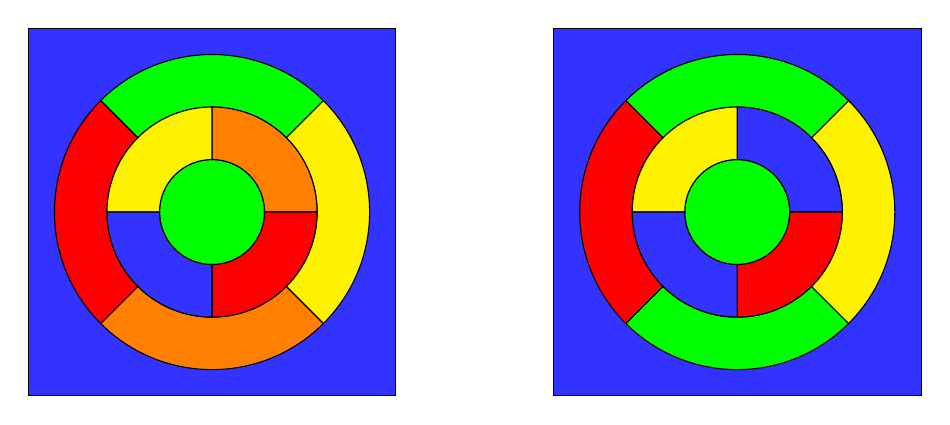
\begin{tikzpicture}[scale=.667]
\draw[fill=blue!80] (-3.5,-3.5) rectangle +(7,7);

\draw[fill=green] (0:1) 
  arc [start angle=0,  end angle=360, radius=1];

\draw[fill=green] (45:2) --
      (45:3)  arc[start angle=45,  end angle=135, radius=3] --
      (135:2) arc[start angle=135, end angle=45,  radius=2];
\draw[fill=orange] (-45:2) --
      (-45:3)  arc[start angle=-45,  end angle=-135, radius=3] --
      (-135:2) arc[start angle=-135, end angle=-45,  radius=2];
\draw[fill=yellow] (45:2) --
      (45:3)  arc[start angle=45,  end angle=-45, radius=3] --
      (-45:2) arc[start angle=-45, end angle=45,  radius=2];
\draw[fill=red] (135:2) --
      (135:3)  arc[start angle=135,  end angle=225, radius=3] --
      (225:2) arc[start angle=225, end angle=135,  radius=2];

\draw[fill=orange] (0:1) --
      (0:2)  arc[start angle=0,  end angle=90, radius=2] --
      (90:1) arc[start angle=90, end angle=0,  radius=1];
\draw[fill=red] (0:1) --
      (0:2)  arc[start angle=0,  end angle=-90, radius=2] --
      (-90:1) arc[start angle=-90, end angle=0,  radius=1];
\draw[fill=yellow] (90:1) --
      (90:2)  arc[start angle=90,  end angle=180, radius=2] --
      (180:1) arc[start angle=180, end angle=90,  radius=1];
\draw[fill=blue!80] (180:1) --
      (180:2)  arc[start angle=180,  end angle=270, radius=2] --
      (270:1) arc[start angle=270, end angle=180,  radius=1];

\begin{scope}[xshift=10cm]
\draw[fill=blue!80] (-3.5,-3.5) rectangle +(7,7);

\draw[fill=green] (0:1) 
  arc [start angle=0,  end angle=360, radius=1];

\draw[fill=green] (45:2) --
      (45:3)  arc[start angle=45,  end angle=135, radius=3] --
      (135:2) arc[start angle=135, end angle=45,  radius=2];
\draw[fill=green] (-45:2) --
      (-45:3)  arc[start angle=-45,  end angle=-135, radius=3] --
      (-135:2) arc[start angle=-135, end angle=-45,  radius=2];
\draw[fill=yellow] (45:2) --
      (45:3)  arc[start angle=45,  end angle=-45, radius=3] --
      (-45:2) arc[start angle=-45, end angle=45,  radius=2];
\draw[fill=red] (135:2) --
      (135:3)  arc[start angle=135,  end angle=225, radius=3] --
      (225:2) arc[start angle=225, end angle=135,  radius=2];

\draw[fill=blue!80] (0:1) --
      (0:2)  arc[start angle=0,  end angle=90, radius=2] --
      (90:1) arc[start angle=90, end angle=0,  radius=1];
\draw[fill=red] (0:1) --
      (0:2)  arc[start angle=0,  end angle=-90, radius=2] --
      (-90:1) arc[start angle=-90, end angle=0,  radius=1];
\draw[fill=yellow] (90:1) --
      (90:2)  arc[start angle=90,  end angle=180, radius=2] --
      (180:1) arc[start angle=180, end angle=90,  radius=1];
\draw[fill=blue!80] (180:1) --
      (180:2)  arc[start angle=180,  end angle=270, radius=2] --
      (270:1) arc[start angle=270, end angle=180,  radius=1];
\end{scope}
\end{tikzpicture}
\end{center}
%\caption{צביעת מפות}\label{f.maps}
%\end{figure}

\textbf{הגדרה:}
\textbf{גרף}
הוא קבוצה של 
\textbf{צמתים}
$V$
וקבוצה של 
\textbf{קשתות}
$E$,
כך שכל קשת מחבר בדיוק שני צמתים.
\textbf{גרף מישורי}
הוא גרף בו שתי קשתות לא חותכות אחת את השניה. בגרף מישורי קטע מהמישור התחום על ידי קבוצה של קשתות נקרא 
\textbf{שטח}.
\textbf{צביעה}
של גרף מישורי היא השמה של צבעים לצמתים כך ששני צמתים המחוברים על ידי קשת צבועים בצבעים שונים.

%\newpage

מפות וגרפים דואליים ונוח יותר לטפל בבעיות צביעה בגרפים ולא במפות.
\begin{theorem}\mbox{}\\
נתונה מפה מישורית, ניתן לבנות גרף מישורי כך שעבור כל צביעה של שטחים במפה קיימת צביעה של הצמתים בגרף, ולהיפך.
\end{theorem}

\textbf{הוכחה:}
בנו צומת עבור כל שטח במפה ובנו קשת בין שני צמתים אם ורק אם קיים גבול בין שני השטחים.
\qed

האיור שלהן
%\ref{f.map-graph}
מראה את הגרף המישורי שניתן לבנות מהמפה המישורית שהבאנו לעיל:
%\begin{figure}[tb]
\begin{center}
\selectlanguage{english}
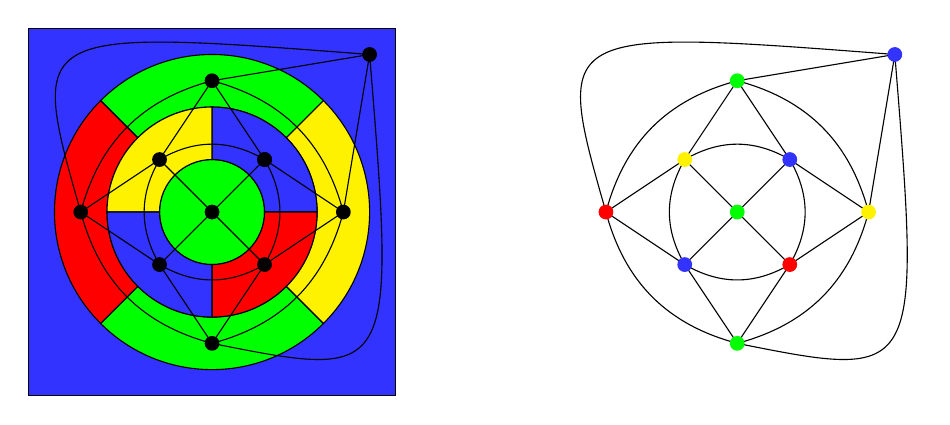
\begin{tikzpicture}[scale=.667]

\draw[fill=blue!80] (-3.5,-3.5) rectangle +(7,7);

\draw[fill=green] (0:1) 
  arc [start angle=0,  end angle=360, radius=1];

\draw[fill=green] (45:2) --
      (45:3)  arc[start angle=45,  end angle=135, radius=3] --
      (135:2) arc[start angle=135, end angle=45,  radius=2];
\draw[fill=green] (-45:2) --
      (-45:3)  arc[start angle=-45,  end angle=-135, radius=3] --
      (-135:2) arc[start angle=-135, end angle=-45,  radius=2];
\draw[fill=yellow] (45:2) --
      (45:3)  arc[start angle=45,  end angle=-45, radius=3] --
      (-45:2) arc[start angle=-45, end angle=45,  radius=2];
\draw[fill=red] (135:2) --
      (135:3)  arc[start angle=135,  end angle=225, radius=3] --
      (225:2) arc[start angle=225, end angle=135,  radius=2];

\draw[fill=blue!80] (0:1) --
      (0:2)  arc[start angle=0,  end angle=90, radius=2] --
      (90:1) arc[start angle=90, end angle=0,  radius=1];
\draw[fill=red] (0:1) --
      (0:2)  arc[start angle=0,  end angle=-90, radius=2] --
      (-90:1) arc[start angle=-90, end angle=0,  radius=1];
\draw[fill=yellow] (90:1) --
      (90:2)  arc[start angle=90,  end angle=180, radius=2] --
      (180:1) arc[start angle=180, end angle=90,  radius=1];
\draw[fill=blue!80] (180:1) --
      (180:2)  arc[start angle=180,  end angle=270, radius=2] --
      (270:1) arc[start angle=270, end angle=180,  radius=1];


\foreach \x/\y/\name in {
    0/0/O,
    3/3/Z,
    1/1/E,-1/1/F,-1/-1/G,1/-1/H,
    0/2.5/A,2.5/0/B,0/-2.5/C,-2.5/0/D,
    } {
  \fill (\x,\y) coordinate(\name) circle(4pt);
}

\draw (E) -- (O) -- (F);
\draw (G) -- (O) -- (H);
\draw (E) to [bend right=30] (F) to [bend right=30] (G) 
          to [bend right=30] (H) to [bend right=30] (E);
\draw (A) -- (E) -- (B) -- (H) -- (C) -- (G) -- (D) -- (F);
\draw (A) to [bend right=30] (D) to [bend right=30] (C) 
          to [bend right=30] (B) to [bend right=30] (A);

\draw (F) -- (A) -- (Z) -- (B);
\draw (C) .. controls (3.5,-3.2) .. (Z);
\draw (D) .. controls (-3.5,3.5) .. (Z);

\begin{scope}[xshift=10cm]

\foreach \x/\y/\name in {
    0/0/O,
    3/3/Z,
    1/1/E,-1/1/F,-1/-1/G,1/-1/H,
    0/2.5/A,2.5/0/B,0/-2.5/C,-2.5/0/D,
    } {
  \coordinate(\name) at (\x,\y);
}

\draw (E) -- (O) -- (F);
\draw (G) -- (O) -- (H);
\draw (E) to [bend right=30] (F) to [bend right=30] (G) 
          to [bend right=30] (H) to [bend right=30] (E);
\draw (A) -- (E) -- (B) -- (H) -- (C) -- (G) -- (D) -- (F);
\draw (A) to [bend right=30] (D) to [bend right=30] (C) 
          to [bend right=30] (B) to [bend right=30] (A);

\draw (F) -- (A) -- (Z) -- (B);
\draw (C) .. controls (3.5,-3.2) .. (Z);
\draw (D) .. controls (-3.5,3.5) .. (Z);

\foreach \cl/\x/\y in {
    green/0cm/0cm,
    blue!80/3cm/3cm,
    blue!80/1cm/1cm,
    yellow/-1cm/1cm,
    blue!80/-1cm/-1cm,
    red/1cm/-1cm,
    green/0cm/2.5cm,
    yellow/2.5cm/0cm,
    green/0cm/-2.5cm,
    red/-2.5cm/0cm
    }
  \fill[\cl] (\x,\y) circle (4pt);
\end{scope}
\end{tikzpicture}
\end{center}
%\caption{גרף שקול למפה}\label{f.map-graph}
%\end{figure}
ניתן להגביל את עצמנו לגרפים שהשטחים שלהם
\textbf{משולשיים}.%
\footnote{%
השטחים הם לא בהכרח 
\textbf{משולשים}
כי הקשתות יכולות להיות עקומות. לפי משפט
\L{F\'{a}ry},
כל גרף מישורי משולשי ניתן להפוך לגרף מישורי שקול עם קשתות ישרות.%
}

האיור השמאלי שלהלן מראה צביעת ריבוע עם שני צבעים, אבל אם 
\textbf{מתלתים}
\L{(triangulate)} 
אותו )איור מרכזי(, חייבים להשתמש בארבעה צבעים. היעד הוא להוכיח 
\textbf{שכל}
גרף ניתן לצבוע בחמישה צבעים, כך שאם הדבר אפשרי בגרף המשולשי, הוא אפשרי גם בגרף המקורי, כי מחיקת הקשתות הנוספות לא מקלקלת את הצביעה )איור ימני(.
\begin{center}
\selectlanguage{english}
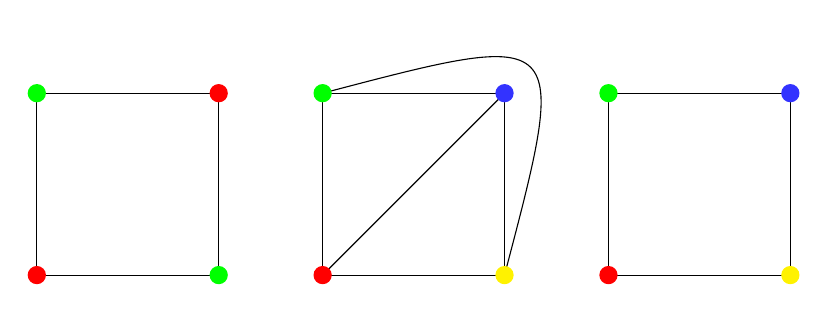
\begin{tikzpicture}[scale=.33]
\draw (-3.5,-3.5) rectangle +(7,7);
\fill[red] (-3.5,-3.5) circle(10pt);
\fill[green] (-3.5,3.5) circle(10pt);
\fill[green] (3.5,-3.5) circle(10pt);
\fill[red] (3.5,3.5) circle(10pt);
\begin{scope}[xshift=11cm]
\draw (-3.5,-3.5) -- (3.5,3.5);
\draw (-3.5,3.5) .. controls (6,6) .. (3.5,-3.5);
\draw (-3.5,-3.5) rectangle +(7,7);
\fill[red] (-3.5,-3.5) circle(10pt);
\fill[green] (-3.5,3.5) circle(10pt);
\fill[yellow] (3.5,-3.5) circle(10pt);
\fill[blue!80] (3.5,3.5) circle(10pt);
\end{scope}
\begin{scope}[xshift=22cm]
\draw (-3.5,-3.5) rectangle +(7,7);
\fill[red] (-3.5,-3.5) circle(10pt);
\fill[green] (-3.5,3.5) circle(10pt);
\fill[yellow] (3.5,-3.5) circle(10pt);
\fill[blue!80] (3.5,3.5) circle(10pt);
\end{scope}
\end{tikzpicture}
\end{center}

\section{הנוסחה של
\L{Euler}}

\begin{theorem}[\L{Euler}]\label{thm.euler}\mbox{}\\
יהי
$G$
גרף מישורי מקושר עם
$V$
צמתים,
$E$
קשתות ו-%
$F$
שטחים. אזי
$V-E+F=2$.
\end{theorem}

\textbf{הוכחה:}
באינדוקציה על מספר הקשתות. אם מספר הקשתות בגרף מישורי מקושר הוא אפס, קיים רק צומת אחד ושטח אחד כך ש-%
$1-0+1=2$.

יהי 
$G$
גרף מישורי מקושר עם 
$V$
צמתים, 
$E$
קשתות ו-%
$F$
שטחים, ומחק קשת 
$e$
המחבר את הצמתים
$v_1,v_2$.


\textbf{מקרה 1:}
הגרף מפסיק להיות מקושר )איור שמאלי(. זהה את
$v_1$
עם
$v_2$
)איור ימני(.
ל-%
$G'$,
הגרף הנוצר, פחות קשתות מ-%
$G$,
הוא גרף מישורי מקושר,
ולכן לפי הנחת האינדוקציה,
$(V-1)-(E-1)+F=2$
כי יש גם צומת אחד פחות. נפשט ונקבל
$V-E+F=2$
עבור
$G$.

\begin{center}
\selectlanguage{english}
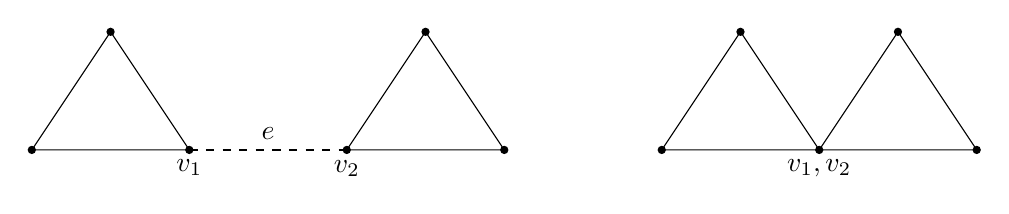
\begin{tikzpicture}
\foreach \x/\y in {0/0, 2/0, 1/1.5,4/0,6/0,5/1.5}
  \fill (\x,\y) circle (1.5pt);
\draw (2,0) -- (1,1.5) -- (0,0) -- (2,0) node[below] {$v_1$};
\draw[dashed,thick] (2,0) -- node[above] {$e$} (4,0) node[below] {$v_2$};
\draw (4,0) -- (6,0) -- (5,1.5) -- (4,0);
\begin{scope}[xshift=8cm]
\foreach \x/\y in {0/0, 2/0, 1/1.5,4/0,3/1.5}
  \fill (\x,\y) circle (1.5pt);
\draw (2,0) -- (1,1.5) -- (0,0) -- (2,0) node[below] {$v_1,v_2$} -- (4,0) -- (3,1.5) -- (2,0);
\end{scope}
\end{tikzpicture}
\end{center}

\textbf{מקרה 2:}
הגרף נשאר מקושר. לגרף הנוצר
$G'$
פחות קשתות מ-%
$G$,
ולכן לפי הנחת האינדוקציה,
$V-(E-1)+(F-1)=2$
כי מחיקת קשת אחת מאחדת שני שטחים לאחד. נפשט ונקבל
$V-E+F=2$ 
עבור
$G$.
\qed

\begin{center}
\selectlanguage{english}
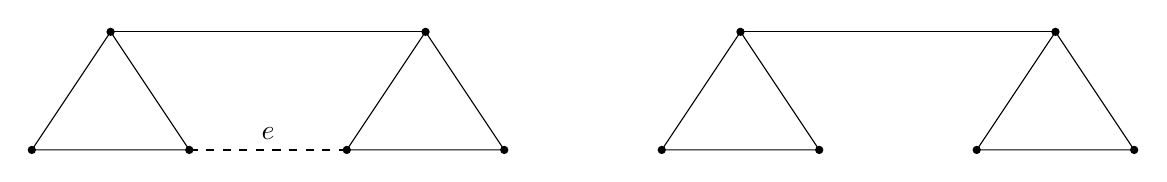
\begin{tikzpicture}
\foreach \x/\y in {0/0, 2/0, 1/1.5,4/0,6/0,5/1.5}
  \fill (\x,\y) circle (1.5pt);
\draw (2,0) -- (1,1.5) -- (0,0) -- (2,0);
\draw[thick,dashed] (2,0) -- node[above] {$e$} (4,0);
\draw (4,0) -- (6,0) -- (5,1.5) -- (4,0);
\draw (1,1.5) -- (5,1.5);
\begin{scope}[xshift=8cm]
\foreach \x/\y in {0/0, 2/0, 1/1.5,4/0,6/0,5/1.5}
  \fill (\x,\y) circle (1.5pt);
\draw (2,0) -- (1,1.5) -- (0,0) -- (2,0);
\draw (4,0) -- (5,1.5) -- (6,0) -- cycle;
\draw (1,1.5) -- (5,1.5);
\end{scope}
\end{tikzpicture}
\end{center}
\begin{theorem}\mbox{}\\
יהי
$G$
גרף מישורי מקושר ומתולת. אזי
$E= 3V-6$.
\end{theorem}
למשל, בגרף המישורי בסעיף
\L{~\ref{s.planar}}
יש
$10$
צמתים ו-%
$24= 3\cdot 10-6$
קשתות.

\textbf{הוכחה:}
כל שטח חסום על ידי שלוש קשתות, כך ש-%
$E=3F/2$
כי כל קשת נספר פעמיים, פעם אחת לכל שטח שהיא חוסמת. לפי נוסחת
\L{Euler}:
\erh{2pt}
\begin{equationarray*}{rcl}
E&=&V+F-2\\
E&=&V+2E/3-2\\
E&=&3V-6\,.
\end{equationarray*}\qed

\begin{theorem}\label{thm.count}\mbox{}\\
יהי
$G$
גרף מישורי מקושר. אזי
$E\leq 3V-6$.
\end{theorem}
עבור הגרף באיור שלהלן,
$E=8\leq 3\cdot 6 - 6= 12$.

\begin{center}
\selectlanguage{english}
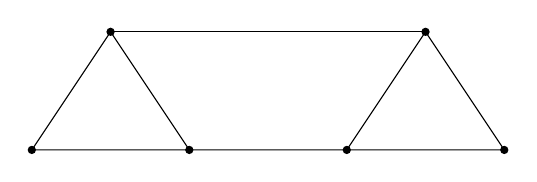
\begin{tikzpicture}
\foreach \x/\y in {0/0, 2/0, 1/1.5,4/0,6/0,5/1.5}
  \fill (\x,\y) circle (1.5pt);
\draw (2,0) -- (1,1.5) -- (0,0) -- (2,0) -- (4,0) -- (6,0) -- (5,1.5) -- (4,0);
\draw (1,1.5) -- (5,1.5);
\end{tikzpicture}
\end{center}

\textbf{הוכחה:}
תלתו את
$G$
כדי לקבל
$G'$.
ב-%
$G'$, $E= 3V-6$
לפי משפט~%
\L{\ref{thm.count}}.
כעת, מחק קשתות מ-%
$G'$
כדי לקבל את
$G$.
מספר הצמתים לא משתנה כך ש-%
$E\leq 3V-6$.\qed

הנה הגרף המתולת שעבורו
$E=3\cdot 6 - 6= 12$.
\begin{center}
\selectlanguage{english}
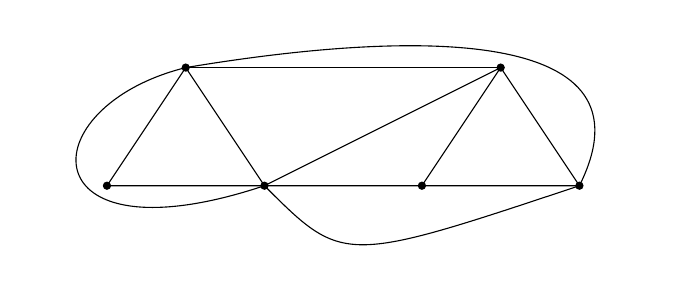
\begin{tikzpicture}
\foreach \x/\y in {0/0, 2/0, 1/1.5,4/0,6/0,5/1.5}
  \fill (\x,\y) circle (1.5pt);
\draw (2,0) -- (1,1.5) -- (0,0) -- (2,0) -- (4,0) -- (6,0) -- (5,1.5) -- (4,0);
\draw (1,1.5) -- (5,1.5);
\draw (2,0) -- (5,1.5);
\draw (2,0) .. controls (-1,-1) and (-1,1) .. (1,1.5);
\draw (2,0) .. controls (3,-1) .. (6,0) .. controls (7,2) and (4,2) .. (1,1.5);
\end{tikzpicture}
\end{center}

\section{גרפים שאינם מישוריים}
נסטה מעט מהסיפור כדי להראות איך ניתן להשתמש במשפטים 
\L{~\ref{thm.euler}}
ו-%
\L{~\ref{thm.count}}
כדי להוכיח שגרפים מסויימים אינם מישוריים.

\begin{theorem}\mbox{}\\
$K_5$,
הגרף השלם עם חמישה צמתים אינו מישורי.
\end{theorem}
%\begin{figure}[bt]
\begin{center}
\selectlanguage{english}
\begin{tikzpicture}[scale=.8]
\node (pentagon) [minimum size=4cm,regular polygon,regular polygon sides=5] at (0,0) {};
\draw (pentagon.corner 1) -- (pentagon.corner 2);
\draw (pentagon.corner 2) -- (pentagon.corner 3);
\draw (pentagon.corner 3) -- (pentagon.corner 4);
\draw (pentagon.corner 4) -- (pentagon.corner 5);
\draw (pentagon.corner 5) -- (pentagon.corner 1);
\draw (pentagon.corner 1) -- (pentagon.corner 3);
\draw (pentagon.corner 1) -- (pentagon.corner 4);
\draw (pentagon.corner 2) -- (pentagon.corner 4);
\draw (pentagon.corner 2) -- (pentagon.corner 5);
\draw (pentagon.corner 3) -- (pentagon.corner 5);

\foreach \corner in {1,2,3,4,5}
  \fill (pentagon.corner \corner) circle (2pt);

\begin{scope}[xshift=8cm]
\node (pentagon) [minimum size=4cm,regular polygon,regular polygon sides=5] at (0,0) {};
\draw (pentagon.corner 1) -- (pentagon.corner 2);
\draw (pentagon.corner 2) -- (pentagon.corner 3);
\draw (pentagon.corner 3) -- (pentagon.corner 4);
\draw (pentagon.corner 4) -- (pentagon.corner 5);
\draw (pentagon.corner 5) -- (pentagon.corner 1);
\draw (pentagon.corner 1) .. controls (-4,1) .. 
      (pentagon.corner 3);
\draw (pentagon.corner 1) .. controls (4,1) ..
      (pentagon.corner 4);
\draw (pentagon.corner 2) -- (pentagon.corner 4);
\draw (pentagon.corner 2) -- (pentagon.corner 5);
\draw (pentagon.corner 3) -- (pentagon.corner 5);

\foreach \corner in {1,2,3,4,5}
  \fill (pentagon.corner \corner) circle (2pt);
\draw (0,-.95) circle(5pt);
\end{scope}
\end{tikzpicture}
\end{center}
%\caption{גרף שלם על עם חמישה קודקודים}\label{f.k5}
%\end{figure}
\textbf{הוכחה:}
עבור
$K_5$, $V=5$
ו-%
$E=10$.
אבל
$10 \not\leq 3\cdot 5 -6=9$.\qed

\begin{theorem}\mbox{}\\
$K_{3,3}$,
הגרף הדו-אזורי עם שלושה צמתים בכל איזור )איור שמאלי(,
אינו מישורי.
\end{theorem}
%\begin{figure}[tb]
\begin{center}
\selectlanguage{english}
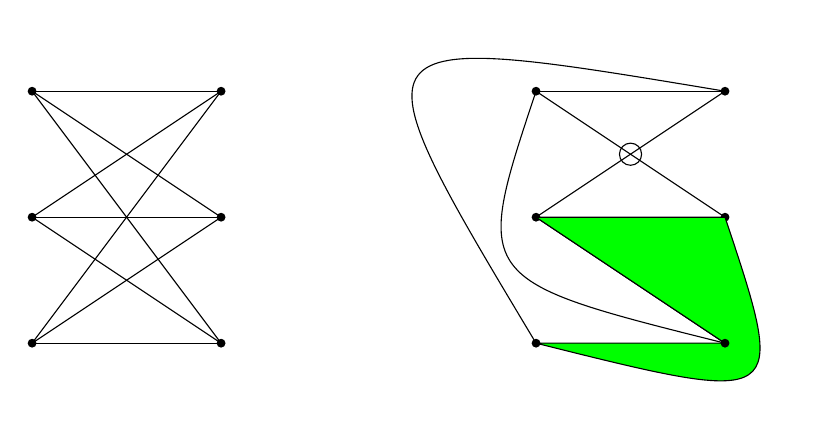
\begin{tikzpicture}[scale=.8]
\foreach \x/\y in {0/0,0/2,0/4,3/0,3/2,3/4}
  \fill (\x,\y) circle (2pt);
\draw (0,0) -- (3,0);
\draw (0,2) -- (3,2);
\draw (0,4) -- (3,4);
\draw (0,0) -- (3,2);
\draw (0,2) -- (3,4);
\draw (0,4) -- (3,0);
\draw (0,0) -- (3,4);
\draw (0,2) -- (3,0);
\draw (0,4) -- (3,2);
\begin{scope}[xshift=8cm]
\foreach \x/\y in {0/0,0/2,0/4,3/0,3/2,3/4}
  \fill (\x,\y) circle (2pt);
\draw (0,4) -- (3,4);
c\draw (0,2) -- (3,4);
\draw (0,4) .. controls (-1,1) .. (3,0);
\draw (0,0) .. controls (-3,5) .. (3,4);
\draw (0,2) -- (3,0);
\draw (0,4) -- (3,2);

\draw[fill=green] (0,0) -- (3,0) -- (3,0) -- (0,2)  -- (3,2) .. controls (4,-1) .. (0,0);
\fill (3,0) circle (2pt);
\draw (1.5,3) circle(5pt);
\end{scope}
\end{tikzpicture}
\end{center}
%\caption{גרף דו-איזורי עם שלושה צמתים בכל איזור}\label{f.k33}
%\end{figure}
\textbf{הוכחה:}
$V=6$
ו-%
$E=9$.
לפי משפט
\L{~\ref{thm.euler}},
$F=E-V+2=9-6+2=5$.
אבל כל שטח תחום על ידי ארבע קשתות )איור ימני(, ולכן
$E=4F/2=(4\cdot 5)/2\neq 9$.\qed

\section{המעלה של הצמתים}

\textbf{הגדרה:}
$d(v)$,
\textbf{המעלה}
של צומת
$v$,
היא מספר הקשתות הנפגשות ב-%
$v$.
עבור הגרף בסעיף
\L{~\ref{s.planar}},
קיימים 
$8$
צמתים בתוך הטבעות, כל אחד ממעלה
$5$.
המעלה של השטח החיצוני ושל המעגל הפנימי הוא 
$4$.
לכן:
\[
\sum_{v\in V} d(v) = 5\cdot 8 + 4\cdot 2=48\,.
\]
נקבל את מספר הקשתות בגרף על ידי חלוקת סכום המעלות ב-%
$2$,
כי כל קשת נספרה פעמיים, פעם אחת עבור כל צומת שהיא נוגעת בו.
הכללת הטיעונים הללו מוכיחה:
\begin{theorem}\label{thm.degrees}\mbox{}\\
יהי
$d_i, i=1,2,3,\ldots,k$
מספרי הצמתים ממעלה
$i$
בגרף מישורי מקושר עם
$V$
צמתים ו-%
$E$ 
קשתות, כאשר
$k$
הוא המעלה הגבוהה ביותר של צומת ב-%
$V$.
אזי:
\[
\sum_{v\in V} d(v) =\sum_{i=1}^{k} i\cdot d_i=2E\,.
\]
\end{theorem}
\vspace*{-6ex}
\begin{theorem}\label{thm.degree5}\mbox{}\\
יהי
$G$
גרף מישורי מקושר עם
$E$
קשתות ו-%
$V$
צמתים, ויהי
$d_i,i=1,\ldots,k$
מספרי ההצמתים ממעלה
$i$,
כאשר
$k$
הוא המעלה הגבוהה ביותר של צומת ב-%
$V$.
אזי חייב להיות צומת
$v$
ב-%
$V$
כך ש-%
$d(v) \leq 5$.
\end{theorem}
\textbf{הוכחה 1:}
ברור שאם יש 
$d_1$
צמתים ממעלה
$1$, $d_2$ 
צמתים ממעלה
$2$, \ldots, $d_k$
צמתים ממעלה
$k$, 
אזי
$V=\sum_{i=1}^{k}d_i$. 
מהמשפטים
\L{~\ref{thm.count}}
ו-%
\L{~\ref{thm.degrees}}
נקבל:
\[
\sum_{i=1}^{k} i\cdot d_i=2E\leq 2(3V-6) = 6V-12=6\sum_{i=1}^{k} d_i -12\,.
\]
מכאן ש:
\[
\sum_{i=1}^{k} i\cdot d_i \leq 6\sum_{i=1}^{k} d_i -12\,,
\]
ו:
\[
\sum_{i=1}^{k} (6-i)d_i\geq 12\,.
\]
בגלל ש-%
$12>0$,
ל-%
$i$
אחד לפחות,
$6-i>0$
ועבור 
$i$
זה,
$i<6$. 
\qed

\textbf{הוכחה 2:}
נחשב את 
\textbf{הממוצע}
של המעלות של הצמתים שהוא סכום המעלות לחלק למספר הצמתים:
\[
d_{\textit{\footnotesize avg}}=\frac{\sum_{i=1}^{k} i\cdot d_i}{V}\,.
\]
אבל סכום המעלות הוא פעמיים מספר הקשתות, ולפי משפט
\L{~\ref{thm.count}}
נקבל:
\[
d_{\textit{\footnotesize avg}}=\frac{2E}{V}\leq \frac{6V-12}{V}=6-\frac{6}{V}<6\,.
\]
אם 
\textbf{הממוצע}
של המעלות הוא פחות משש, חייב להיות צומת אחד לפחות ממעלה פחות משש.
\qed


עבור הגרף בסעיף
\L{~\ref{s.planar}},
סכום המעלות הוא
$8\cdot 5 + 2\cdot 4=48$.
יש 
$10$
צמתים, כך שממוצע המעלות שלו הוא
$\frac{48}{10}=4.8$
וחייב להיות צומת ממעלה 
$4$
או פחות.

\section{משפט ששת הצבעים}

\begin{theorem}\label{thm.sixcolor}\mbox{}\\
כל גרף מישורי ניתן לצביעה בששה צבעים.
\end{theorem}
\textbf{הוכחה:}
באינדוקציה על מספר הצמתים ב-%
$G$.
אם לגרף ששה צמתים או פחות, ברור שניתן לצבוע את הגרף בששה צבעים.

יהי
$G$
גרף מישורי. לפי משפט
\L{~\ref{thm.degree5}}
קיים צומת
$v$
ממעלה חמש או פחות. מחק צומת
$v$
כדי לקבל את הגרף
$G'$.
לפי הנחת האינדוקציה, ניתן לצבוע את
$G'$
עם ששה צבעים, אבל ל-%
$v$
חמישה שכנים לכל היותר שצבועים בחמישה 
צבעים לכל היותר, כך שנשאר צבע ששי שניתן לצבוע בו את
$v$. \qed

\begin{center}
\selectlanguage{english}
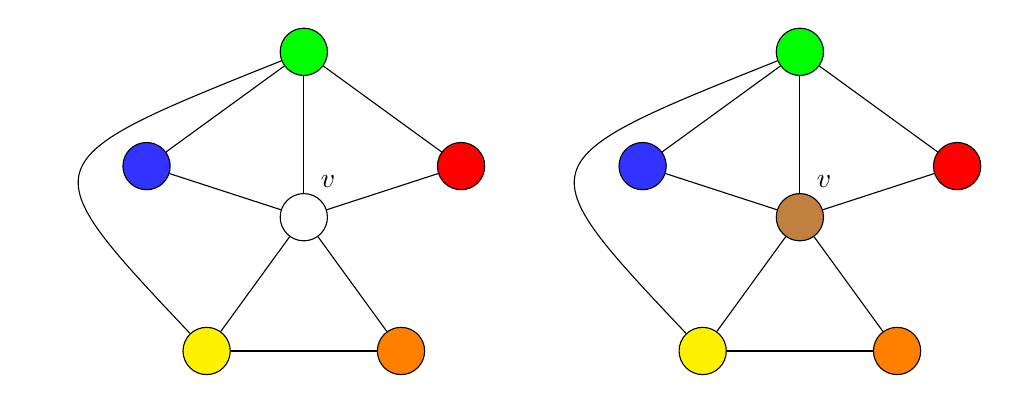
\begin{tikzpicture}[scale=.7,minimum size=6mm,inner sep=0pt]
\foreach \name/\color/\theta in
    {A/red/18,B/green/90,C/blue!80/162,D/yellow/234,E/orange/306}
  \node[circle,draw,fill=\color] (\name) at (\theta:3) {};
\node[circle,draw] (O) at (0,0) {};
\node[above right,yshift=4pt] at (O) {$v$};
\foreach \name in {A,B,C,D,E}
  \draw (O) -- (\name);
\foreach \i/\j in {A/B,B/C,D/E}
  \draw (\i) -- (\j);
\draw (B) .. controls (-5,1) .. (D);
\begin{scope}[xshift=9cm]
\foreach \name/\color/\theta in
    {A/red/18,B/green/90,C/blue!80/162,D/yellow/234,E/orange/306}
  \node[circle,draw,fill=\color] (\name) at (\theta:3) {};
\node[circle,draw,fill=brown] (O) at (0,0) {};
\node[above right,yshift=4pt] at (O) {$v$};
\foreach \name in {A,B,C,D,E}
  \draw (O) -- (\name);
\foreach \i/\j in {A/B,B/C,D/E}
  \draw (\i) -- (\j);
\draw (B) .. controls (-5,1) .. (D);
\end{scope}
\end{tikzpicture}
\end{center}


\section{משפט חמשת הצבעים}

\textbf{הגדרה:}
יהי
$G$
גרף מישורי מקושר צבוע. 
$G'$
הוא
\textbf{שרשרת}
אם ורק אם
$G'$
הוא תת-גרף מקסימלי של
$G$
הצבוע בשני צבעים.%
\footnote{%
השרשרת נקראת גם
\textbf{שרשרת \L{Kempe}}
כי היא הוגדרה על ידי
\L{Alfred Kempe}
בהוכחה השגויה שלו למשפט ארבעת הצבעים. ראו סעיף~%
\L{\ref{s.kempe}}.}

\begin{theorem}\label{thm.fivecolor}\mbox{}\\
כל גרף מישורי 
$G$
ניתן לצבוע בחמישה צבעים.
\end{theorem}

\textbf{הוכחה:}
באינדקציה על מספר הצמתים. נכונות המשפט ברורה עבור גרף מישורי עם חמישה צמתים או פחות.

יהי
$G$
גרף מישורי. לפי משפט
\L{~\ref{thm.degree5}}
קיים צומת
$v$
ממעלה חמש או פחות. מחק את הצומת
$v$
כדי לקבל את הגרף
$G'$.
לפי הנחת האינדוקציה, ניתן לצבוע את
$G'$
עם חמישה צבעים או פחות:


%\begin{figure}[tb]
\begin{center}
\selectlanguage{english}
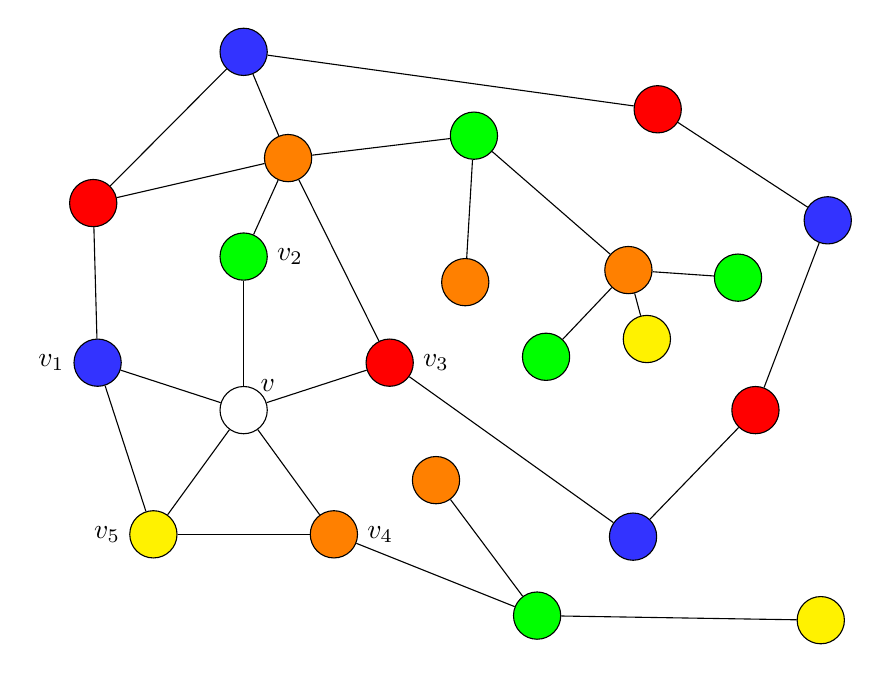
\begin{tikzpicture}[scale=.65,minimum size=6mm,inner sep=0pt]
\foreach \name/\color/\theta in
    {A/red/18,B/green/90,C/blue!80/162,D/yellow/234,E/orange/306}
  \node[circle,draw,fill=\color] (\name) at (\theta:3) {};
\node[circle,draw] (O) at (0,0) {};
\node[above right] at (O) {$v$};

\node[right,xshift=8pt] at (A) {$v_3$};
\node[right,xshift=8pt] at (B) {$v_2$};
\node[left,,xshift=-8pt] at (C) {$v_1$};
\node[left,,xshift=-8pt] at (D) {$v_5$};
\node[right,xshift=8pt] at (E) {$v_4$};

\foreach \name in {A,B,C,D,E}
  \draw (O) -- (\name);
  
\node[circle,draw,fill=red]  (X1) at (126:5) {};
\node[circle,draw,fill=blue!80] (X2) at (90:7)  {};
\node[circle,draw,fill=red]  (X3) at (36:10) {};
\node[circle,draw,fill=blue!80] (X4) at (18:12) {};
\node[circle,draw,fill=red]  (X5) at (0:10) {};
\node[circle,draw,fill=blue!80] (X6) at (-18:8) {};
\draw (C)  -- (X1);
\draw (X1) -- (X2);
\draw (X2) -- (X3);
\draw (X3) -- (X4);
\draw (X4) -- (X5);
\draw (X5) -- (X6);
\draw (X6) -- (A);

\node[circle,draw,fill=orange]  (Y1)  at (80:5) {};
\node[circle,draw,fill=green]   (Y2)  at (50:7)  {};
\node[circle,draw,fill=orange]  (Y3A) at (20:8) {};
\node[circle,draw,fill=orange]  (Y3B) at (30:5) {};
\node[circle,draw,fill=green]   (Y4A) at (10:6) {};
\node[circle,draw,fill=yellow]   (Y4B) at (10:8) {};
\node[circle,draw,fill=green]   (Y4C) at (15:10) {};
\node[circle,draw,fill=green]   (Y5)  at (-35:7) {};
\node[circle,draw,fill=yellow]  (Y6A) at (-20:12) {};
\node[circle,draw,fill=orange]  (Y6B) at (-20:4) {};
\draw (B)  -- (Y1);
\draw (Y1) -- (Y2);
\draw (Y2) -- (Y3A);
\draw (Y2) -- (Y3B);
\draw (Y3A) -- (Y4A);
\draw (Y3A) -- (Y4B);
\draw (Y3A) -- (Y4C);
\draw (E)  -- (Y5);
\draw (Y5) -- (Y6A);
\draw (Y5) -- (Y6B);
\draw (A) -- (Y1);
\draw (X2) -- (Y1);
\draw (X1) -- (Y1);
\draw (D) -- (E);
\draw (D) -- (C);
\end{tikzpicture}
\end{center}
%\caption{לצומת $v$ חמש שכנים לכל היותר}\label{f.five1}
%\end{figure}

ב-%
$G$,
אם המעלה של
$v$
היא פחות מחמש,
או אם
$v_1,\ldots,v_5$,
השכנים של
$v$,
צבועים עם ארבעה צבעים או פחות, ניתן לצבוע את
$v$
עם הצבע החמישי.
אחרת, הצמתים
$v_1,\ldots,v_5$
צבועים בצבעים שונים ב-%
$G'$
כמו באיור.

הצומת
$v_1$
צבוע בכחול והצומת 
$v_3$
צבוע באדום, ויש שרשרת הכחול-אדום המכילה אותם. על ידי הוספת הצומת 
$v$
והקשתות
$\overline{vv_1},\overline{vv_3}$
לשרשרת, נקבל מסלול סגור
$P$
)המסומן בקו כפול( שמחלק את המישור לשטח "פנימי" ולשטח "חיצוני" )אויר~%
\ref{f.five2}(.

\begin{figure}[tb]
\begin{center}
\selectlanguage{english}
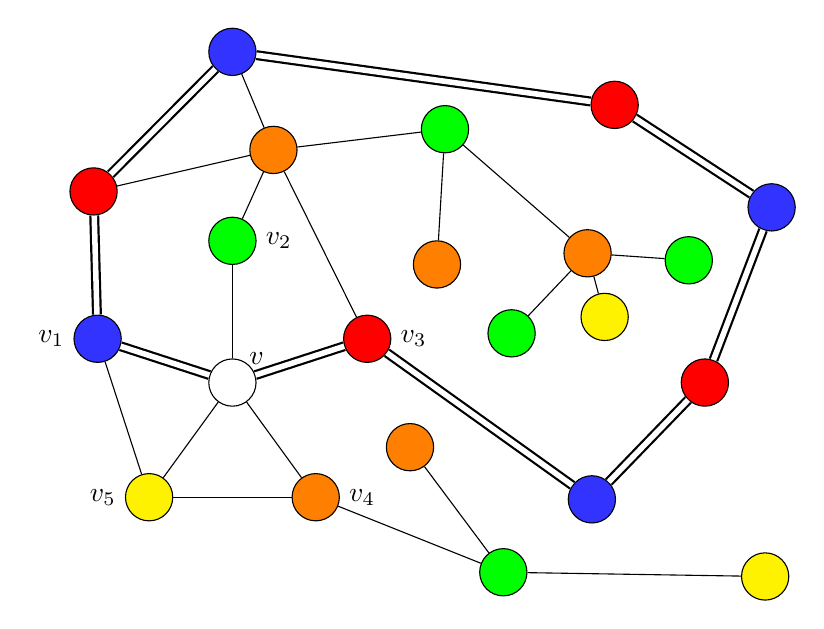
\begin{tikzpicture}[scale=.6,minimum size=6mm,inner sep=0pt]
\foreach \name/\color/\theta in
    {A/red/18,B/green/90,C/blue!80/162,D/yellow/234,E/orange/306}
  \node[circle,draw,fill=\color] (\name) at (\theta:3) {};
\node[circle,draw] (O) at (0,0) {};
\node[above right] at (O) {$v$};

\node[right,xshift=8pt] at (A) {$v_3$};
\node[right,xshift=8pt] at (B) {$v_2$};
\node[left,,xshift=-8pt] at (C) {$v_1$};
\node[left,,xshift=-8pt] at (D) {$v_5$};
\node[right,xshift=8pt] at (E) {$v_4$};

\foreach \name in {A,B,C,D,E}
  \draw (O) -- (\name);
  
\node[circle,draw,fill=red]  (X1) at (126:5) {};
\node[circle,draw,fill=blue!80] (X2) at (90:7)  {};
\node[circle,draw,fill=red]  (X3) at (36:10) {};
\node[circle,draw,fill=blue!80] (X4) at (18:12) {};
\node[circle,draw,fill=red]  (X5) at (0:10) {};
\node[circle,draw,fill=blue!80] (X6) at (-18:8) {};
\draw[thick,double distance=2pt] (C)  -- (X1);
\draw[thick,double distance=2pt] (X1) -- (X2);
\draw[thick,double distance=2pt] (X2) -- (X3);
\draw[thick,double distance=2pt] (X3) -- (X4);
\draw[thick,double distance=2pt] (X4) -- (X5);
\draw[thick,double distance=2pt] (X5) -- (X6);
\draw[thick,double distance=2pt] (X6) -- (A);
\draw[thick,double distance=2pt] (A) -- (O) -- (C);

\node[circle,draw,fill=orange]  (Y1)  at (80:5) {};
\node[circle,draw,fill=green]   (Y2)  at (50:7)  {};
\node[circle,draw,fill=orange]  (Y3A) at (20:8) {};
\node[circle,draw,fill=orange]  (Y3B) at (30:5) {};
\node[circle,draw,fill=green]   (Y4A) at (10:6) {};
\node[circle,draw,fill=yellow]   (Y4B) at (10:8) {};
\node[circle,draw,fill=green]   (Y4C) at (15:10) {};
\node[circle,draw,fill=green]   (Y5)  at (-35:7) {};
\node[circle,draw,fill=yellow]  (Y6A) at (-20:12) {};
\node[circle,draw,fill=orange]  (Y6B) at (-20:4) {};
\draw (B)  -- (Y1);
\draw (Y1) -- (Y2);
\draw (Y2) -- (Y3A);
\draw (Y2) -- (Y3B);
\draw (Y3A) -- (Y4A);
\draw (Y3A) -- (Y4B);
\draw (Y3A) -- (Y4C);
\draw (E)  -- (Y5);
\draw (Y5) -- (Y6A);
\draw (Y5) -- (Y6B);
\draw (A) -- (Y1);
\draw (X2) -- (Y1);
\draw (X1) -- (Y1);
\draw (D) -- (E);
\draw (D) -- (C);
\end{tikzpicture}
\end{center}
\caption{מסלול מחלק את המישור לחלק פנימי ולחלק חיצוני}\label{f.five2}
\end{figure}
כעת נתבונן בצומת
$v_2$
הצבוע ירוק ובצומת
$v_4$
הצבוע כתום. הצמתים הללו 
\textbf{אינם}
יכולים להיות בשרשרת ירוק-כתום אחת, כי 
$v_2$
נמצא 
\textbf{בתוך}
$P$
ו-%
$v_4$
נמצא
\textbf{מחוץ}
ל-%
$P$,
ולכן כל מסלול המחבר אותם חייב לחתוך את
$P$,
הסותר את ההנחה שהגרף מישורי.%
\footnote{%
טענה זו נובעת מה-%
\L{\emph{Jordan curve theorem}},
שהוא ברור באופן אינטואיטיבי, אבל קשה מאוד להוכיח.%
}
באיור~%
\ref{f.five3}
אפשר לראות שתי שרשראות ירוק-כתום המכילות את
$v_2$
ו-%
$v_4$
שאינן מחוברות )מסומנות בקו מקווקוו כפול(.
\begin{figure}[tb]
\begin{center}
\selectlanguage{english}
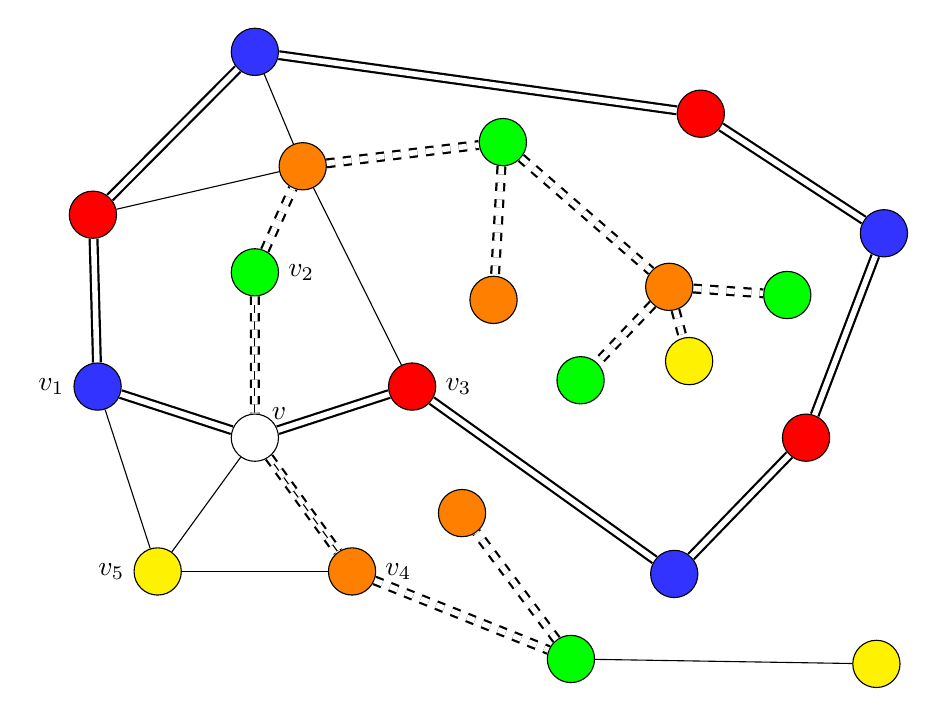
\begin{tikzpicture}[scale=.7,minimum size=6mm,inner sep=0pt]
\foreach \name/\color/\theta in
    {A/red/18,B/green/90,C/blue!80/162,D/yellow/234,E/orange/306}
  \node[circle,draw,fill=\color] (\name) at (\theta:3) {};
\node[circle,draw] (O) at (0,0) {};
\node[above right] at (O) {$v$};

\node[right,xshift=8pt] at (A) {$v_3$};
\node[right,xshift=8pt] at (B) {$v_2$};
\node[left,,xshift=-8pt] at (C) {$v_1$};
\node[left,,xshift=-8pt] at (D) {$v_5$};
\node[right,xshift=8pt] at (E) {$v_4$};

\foreach \name in {A,B,C,D,E}
  \draw (O) -- (\name);
  
\node[circle,draw,fill=red]  (X1) at (126:5) {};
\node[circle,draw,fill=blue!80] (X2) at (90:7)  {};
\node[circle,draw,fill=red]  (X3) at (36:10) {};
\node[circle,draw,fill=blue!80] (X4) at (18:12) {};
\node[circle,draw,fill=red]  (X5) at (0:10) {};
\node[circle,draw,fill=blue!80] (X6) at (-18:8) {};

\draw[thick,double distance=2pt] (C)  -- (X1);
\draw[thick,double distance=2pt] (X1) -- (X2);
\draw[thick,double distance=2pt] (X2) -- (X3);
\draw[thick,double distance=2pt] (X3) -- (X4);
\draw[thick,double distance=2pt] (X4) -- (X5);
\draw[thick,double distance=2pt] (X5) -- (X6);
\draw[thick,double distance=2pt] (X6) -- (A);
\draw[thick,double distance=2pt] (A) -- (O) -- (C);

\node[circle,draw,fill=orange]  (Y1)  at (80:5) {};
\node[circle,draw,fill=green]   (Y2)  at (50:7)  {};
\node[circle,draw,fill=orange]  (Y3A) at (20:8) {};
\node[circle,draw,fill=orange]  (Y3B) at (30:5) {};
\node[circle,draw,fill=green]   (Y4A) at (10:6) {};
\node[circle,draw,fill=yellow]   (Y4B) at (10:8) {};
\node[circle,draw,fill=green]   (Y4C) at (15:10) {};
\node[circle,draw,fill=green]   (Y5)  at (-35:7) {};
\node[circle,draw,fill=yellow]  (Y6A) at (-20:12) {};
\node[circle,draw,fill=orange]  (Y6B) at (-20:4) {};
\draw[thick,dashed,double distance=2pt] (B)  -- (O) -- (E);
\draw[thick,dashed,double distance=2pt] (B)  -- (Y1);
\draw[thick,dashed,double distance=2pt] (Y1) -- (Y2);
\draw[thick,dashed,double distance=2pt] (Y2) -- (Y3A);
\draw[thick,dashed,double distance=2pt] (Y2) -- (Y3B);
\draw[thick,dashed,double distance=2pt] (Y3A) -- (Y4A);
\draw[thick,dashed,double distance=2pt] (Y3A) -- (Y4B);
\draw[thick,dashed,double distance=2pt] (Y3A) -- (Y4C);
\draw[thick,dashed,double distance=2pt] (E)  -- (Y5);
\draw[thick,dashed,double distance=2pt] (Y5) -- (Y6B);
\draw (Y5) -- (Y6A);
\draw (A) -- (Y1);
\draw (X2) -- (Y1);
\draw (X1) -- (Y1);
\draw (D) -- (E);
\draw (D) -- (C);
\end{tikzpicture}
\end{center}
\caption{שרשראות לא מחוברות}\label{f.five3}
\end{figure}

נחליף ביניהם את שני ההצבעים בשרשרת המכילה את
$v_2$
)איור~%
\ref{f.five4}(.
עדיין ניתן לצבוע את
$G'$
עם חמישה צבעים.
$v_2$
ו-%
$v_4$
שניהם צבועים בכתום, וניתן לצבוע את
$v$
בירוק כדי לקבל צביעה של
$G$
עם חמישה צבעים.
\qed

\begin{figure}[tb]
\begin{center}
\selectlanguage{english}
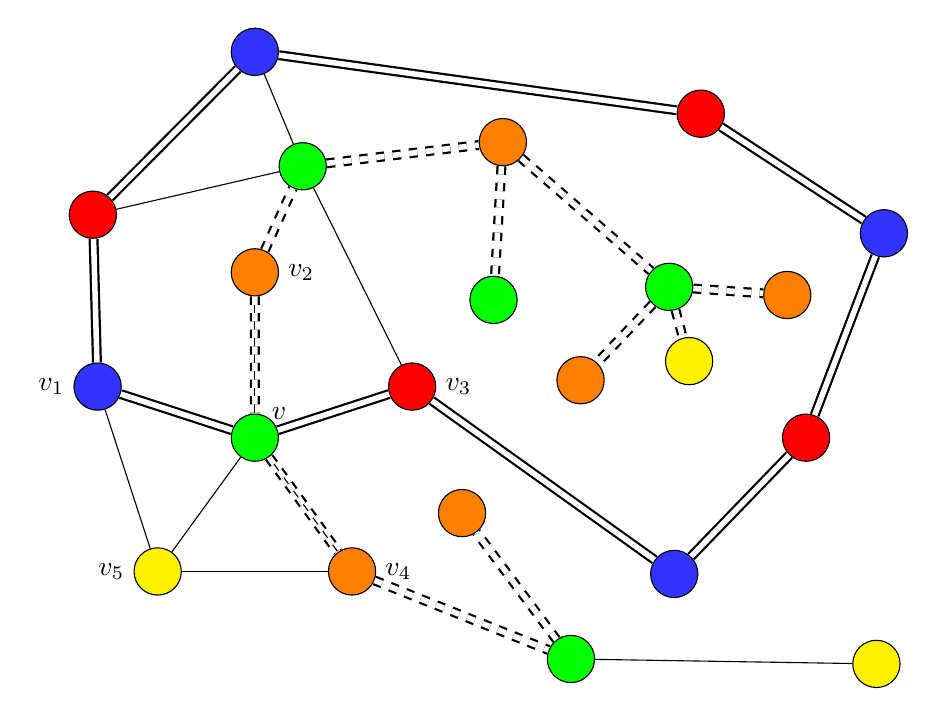
\begin{tikzpicture}[scale=.7,minimum size=6mm,inner sep=0pt]
\foreach \name/\color/\theta in
    {A/red/18,B/orange/90,C/blue!80/162,D/yellow/234,E/orange/306}
  \node[circle,draw,fill=\color] (\name) at (\theta:3) {};
\node[circle,draw,fill=green] (O) at (0,0) {};
\node[above right] at (O) {$v$};

\node[right,xshift=8pt] at (A) {$v_3$};
\node[right,xshift=8pt] at (B) {$v_2$};
\node[left,,xshift=-8pt] at (C) {$v_1$};
\node[left,,xshift=-8pt] at (D) {$v_5$};
\node[right,xshift=8pt] at (E) {$v_4$};

\foreach \name in {A,B,C,D,E}
  \draw (O) -- (\name);
  
\node[circle,draw,fill=red]  (X1) at (126:5) {};
\node[circle,draw,fill=blue!80] (X2) at (90:7)  {};
\node[circle,draw,fill=red]  (X3) at (36:10) {};
\node[circle,draw,fill=blue!80] (X4) at (18:12) {};
\node[circle,draw,fill=red]  (X5) at (0:10) {};
\node[circle,draw,fill=blue!80] (X6) at (-18:8) {};

\draw[thick,double distance=2pt] (C)  -- (X1);
\draw[thick,double distance=2pt] (X1) -- (X2);
\draw[thick,double distance=2pt] (X2) -- (X3);
\draw[thick,double distance=2pt] (X3) -- (X4);
\draw[thick,double distance=2pt] (X4) -- (X5);
\draw[thick,double distance=2pt] (X5) -- (X6);
\draw[thick,double distance=2pt] (X6) -- (A);
\draw[thick,double distance=2pt] (A) -- (O) -- (C);

\node[circle,draw,fill=green]  (Y1)  at (80:5) {};
\node[circle,draw,fill=orange]   (Y2)  at (50:7)  {};
\node[circle,draw,fill=green]  (Y3A) at (20:8) {};
\node[circle,draw,fill=green]  (Y3B) at (30:5) {};
\node[circle,draw,fill=orange]   (Y4A) at (10:6) {};
\node[circle,draw,fill=yellow]   (Y4B) at (10:8) {};
\node[circle,draw,fill=orange]   (Y4C) at (15:10) {};
\node[circle,draw,fill=green]   (Y5)  at (-35:7) {};
\node[circle,draw,fill=yellow]  (Y6A) at (-20:12) {};
\node[circle,draw,fill=orange]  (Y6B) at (-20:4) {};

\draw[thick,dashed,double distance=2pt] (B)  -- (O) -- (E);
\draw[thick,dashed,double distance=2pt] (B)  -- (Y1);
\draw[thick,dashed,double distance=2pt] (Y1) -- (Y2);
\draw[thick,dashed,double distance=2pt] (Y2) -- (Y3A);
\draw[thick,dashed,double distance=2pt] (Y2) -- (Y3B);
\draw[thick,dashed,double distance=2pt] (Y3A) -- (Y4A);
\draw[thick,dashed,double distance=2pt] (Y3A) -- (Y4B);
\draw[thick,dashed,double distance=2pt] (Y3A) -- (Y4C);
\draw[thick,dashed,double distance=2pt] (E)  -- (Y5);
\draw[thick,dashed,double distance=2pt] (Y5) -- (Y6B);

\draw (Y5) -- (Y6A);
\draw (A) -- (Y1);
\draw (X2) -- (Y1);
\draw (X1) -- (Y1);
\draw (D) -- (E);
\draw (D) -- (C);
\end{tikzpicture}
\end{center}
\caption{החלפת צבעים בשרשרת אחת}\label{f.five4}
\end{figure}

%%%%%%%%%%%%%%%%%%%%%%%%%%%%%%%%%%%%%%%%%%%%%%%%%%%%%%%%%%%
%%%%%%%%%%%%%%%%%%%%%%%%%%%%%%%%%%%%%%%%%%%%%%%%%%%%%%%%%%%


\section{ההוכחה השגויה של
\L{Kempe}}
\label{s.kempe}

משפט ארבעת הצבעים הוצג כהשערה ב-%
$1852$.
ב-%
$1879$
\L{Alfred B. Kempe}
פרסם הוכחה, אבל ב-%
$1890$,
\L{Percy J. Heawood}
מצא בה שגיאה. העבודה של
\L{Kempe}
חשובה כי: 
$(1)$
ההוכחה נכונה עבור חמישה צבעים, ו-%
$(2)$
בהוכחה שלו הוא המציא את הרעיונות הבסיסיים ששימשו את
\L{Appel}
ו-%
\L{Haken}
בהוכחה הנכונה שלהם שפורסמה ב-%
$1976$.

\textbf{"הוכחה":}
רוב ההוכחה זהה להוכחה של משפט חמשת הצבעים. המקרה החדש הוא צומת 
$v$
עם חמישה שכנים שלפי ההנחה האינדוקטיבית ניתן לצבוע אותם
\textbf{בארבעה}
צבעים לאחר מחיקת הצומת
$v$.

בגרף השמאלי של איור %
\ref{f.kempe1}
קיימים שני צמתים
$v_2,v_5$
הצבועים בכחול. נתבונן עכשיו בשרשרת הכחול-ירוק המכילה את 
$v_2$
ובשרשרת הכחול-צהוב המכילה את
$v_5$.
השרשרת הכחול-ירוק נמצאת מתוך המסלול הסגור המוגדר על ידי השרשרת האדום-צהוב שמכילה את
$v_1,v_3$
)מסומן בקו כפול(,
והשרשרת הכחול-צהוב נמצאת בתוך המסלול הסגור המוגדר על ידי השרשרת האדום-ירוק המכילה את
$v_1,v_4$
(מסומן בקו כפול מקווקוו(.

נחליף את הצבעים בשרשרת הכחול-ירוק ובשרשרת הכחול-צהוב )איור ימני(. השכנים של
$v$
צבועים בשלושה צבעים )אדום, ירוק צהוב( וניתן לצבוע את
$v$
בכחול.
\qed
\begin{figure}
\begin{center}
\selectlanguage{english}
\begin{tikzpicture}[scale=.6,minimum size=6mm,inner sep=0pt]

% Draw center node and adjacent nodes
\foreach \name/\color/\theta in
    {A/yellow/18,B/blue!80/90,C/red/162,D/blue!80/234,E/green/306}
  \node[circle,draw,fill=\color] (\name) at (\theta:3) {};
\node[circle,draw] (O) at (0,0) {};
\node[above right]     at (O) {$v$};

\node[right,xshift=10pt] at (A) {$v_3$};
\node[left,xshift=-8pt]  at (B) {$v_2$};
\node[left,xshift=-8pt]  at (C) {$v_1$};
\node[left,xshift=-8pt]  at (D) {$v_5$};
\node[right,xshift=8pt]  at (E) {$v_4$};

% Draw red-yellow path
\node[circle,draw,fill=yellow]  (X1) at (126:5) {};
\node[circle,draw,fill=red] (X2) at (45:8)  {};

\draw[thick,double distance=2pt] 
  (C) -- (X1) -- (X2) -- (A) -- (O);
\draw[thick,double distance=6pt] (O) -- (C);

% Draw blue-green nodes within red-yellow path
\node[circle,draw,fill=green] (Y1)  at (50:5) {};

% Draw red-green path
\node[circle,draw,fill=green] (Z1)  at (-160:5) {};
\node[circle,draw,fill=red]   (Z2)  at (-80:6)  {};

%\draw[thick,dashed,double distance=6pt] (O) -- (C);
\draw[thick,dashed,double distance=2pt] 
  (O) -- (C) -- (Z1) -- (Z2) -- (E) -- (O);

% Draw blue-yellow nodes within red-green path
\node[circle,draw,fill=yellow]   (U1)  at (-90:4)  {};

% Connect adjacent nodes not in paths
\draw (X1) -- (B) -- (Y1) -- (A) -- (B) -- 
      (C) -- (D) -- (E) -- (A);
\draw (Z2) -- (U1) -- (D) -- (O) -- (B);

%\end{tikzpicture}
%\end{center}

\begin{scope}[xshift=12cm]
%\begin{center}
%\begin{tikzpicture}[scale=.6,minimum size=6mm,inner sep=0pt]

% Draw center node and adjacent nodes
\foreach \name/\color/\theta in
    {A/yellow/18,B/green/90,C/red/162,D/yellow/234,E/green/306}
  \node[circle,draw,fill=\color] (\name) at (\theta:3) {};
\node[circle,draw,fill=blue!80] (O) at (0,0) {};
\node[above right]     at (O) {$v$};

\node[right,xshift=10pt] at (A) {$v_3$};
\node[left,xshift=-8pt]  at (B) {$v_2$};
\node[left,xshift=-8pt]  at (C) {$v_1$};
\node[left,xshift=-8pt]  at (D) {$v_5$};
\node[right,xshift=8pt]  at (E) {$v_4$};

% Draw red-yellow path
\node[circle,draw,fill=yellow]  (X1) at (126:5) {};
\node[circle,draw,fill=red] (X2) at (45:8)  {};

\draw[thick,double distance=2pt] 
  (C) -- (X1) -- (X2) -- (A) -- (O);
\draw[thick,double distance=6pt] (O) -- (C);

% Draw blue-green nodes within red-yellow path
\node[circle,draw,fill=blue!80] (Y1)  at (50:5) {};

% Draw red-green path
\node[circle,draw,fill=green] (Z1)  at (-160:5) {};
\node[circle,draw,fill=red]   (Z2)  at (-80:6)  {};

\draw[thick,dashed,double distance=2pt] 
  (O) -- (C) -- (Z1) -- (Z2) -- (E) -- (O);

% Draw blue-yellow nodes within red-green path
\node[circle,draw,fill=blue!80]   (U1)  at (-90:4)  {};

% Connect adjacent nodes not in paths
\draw (X1) -- (B) -- (Y1) -- (A) -- (B) -- 
      (C) -- (D) -- (E) -- (A);
\draw (Z2) -- (U1) -- (D) -- (O) -- (B);
\end{scope}
\end{tikzpicture}
\end{center}
\caption{ההוכחה המוטעת של \L{Kempe}}\label{f.kempe1}
\end{figure}

\L{Heawood}
שם לב שלמסלולים הסגורים, המוגדרים על ידי השרשראות האדום-צהוב והאדום-ירוק, ייתכן שיש צמתים אדומים משותפים )%
$v_1$
והצומת האדום מתחת ל-%
$v_4$
בגרף השמאלי של איור~%
\ref{f.kempe2}(.
כאשר מחליפים צבעים בשרשראות הכחול-ירוק והכחול-צהוב, יש אפשרות שיהיו צמתים צבועים בכחול הקשורים בקשת )איור ימני(, כך שהצביעה כבר לא חוקית.
\begin{figure}[tb]
\begin{center}
\selectlanguage{english}
\begin{tikzpicture}[scale=.6,minimum size=6mm,inner sep=0pt]

% Draw center node and adjacent nodes
\foreach \name/\color/\theta in
    {A/yellow/18,B/blue!80/90,C/red/162,D/blue!80/234,E/green/306}
  \node[circle,draw,fill=\color] (\name) at (\theta:3) {};
\node[circle,draw] (O) at (0,0) {};
\node[above right]     at (O) {$v$};

\node[right,xshift=10pt] at (A) {$v_3$};
\node[right,xshift=8pt]  at (B) {$v_2$};
\node[above right,xshift=8pt]  at (C) {$v_1$};
\node[below right,yshift=-8pt] at (D) {$v_5$};
\node[right,xshift=8pt]  at (E) {$v_4$};

% Draw red-yellow path
\node[circle,draw,fill=yellow] (X1) at (-170:5) {};
\node[circle,draw,fill=red]    (X2) at (-80:7)  {};

\draw[thick,double distance=2pt] (A) -- (O);
\draw[thick,double distance=6pt] (O) -- (C);
\draw[thick,double distance=2pt] (C) --(X1) -- (X2);
\draw[thick,double distance=2pt,bend right=40] (X2) to (A);

% Draw red-green path
\node[circle,draw,fill=green] (Y1) at (100:6)  {};

\draw[dashed,thick,double distance=2pt] (O) -- (C) -- (Y1);
\draw[dashed,thick,double distance=2pt] 
  (Y1) .. controls (40:10) and (-50:9) .. (X2);
\draw[dashed,thick,double distance=2pt] (X2) -- (E) -- (O);

% Draw adjacent nodes
\draw (X1) -- (D) -- (O) -- (B) -- (Y1) -- (X1);

%\end{tikzpicture}
%\end{center}

\begin{scope}[xshift=12cm]
%\begin{center}
%\begin{tikzpicture}[scale=.6,minimum size=6mm,inner sep=0pt]

% Draw center node and adjacent nodes
\foreach \name/\color/\theta in
    {A/yellow/18,B/green/90,C/red/162,D/yellow/234,E/green/306}
  \node[circle,draw,fill=\color] (\name) at (\theta:3) {};
\node[circle,draw,fill=blue!80] (O) at (0,0) {};
\node[above right]     at (O) {$v$};

\node[right,xshift=10pt] at (A) {$v_3$};
\node[right,xshift=8pt]  at (B) {$v_2$};
\node[above right,xshift=8pt]  at (C) {$v_1$};
\node[below right,yshift=-8pt] at (D) {$v_5$};
\node[right,xshift=8pt]  at (E) {$v_4$};


% Draw red-yellow path
\node[circle,draw,fill=blue!80] (X1) at (-170:5) {};
\node[circle,draw,fill=red]  (X2) at (-80:7)  {};

\draw[thick,double distance=2pt] (A) -- (O);
\draw[thick,double distance=6pt] (O) -- (C);
\draw[thick,double distance=2pt] (C) --(X1) -- (X2);
\draw[thick,double distance=2pt,bend right=40] (X2) to (A);

% Draw red-green path
\node[circle,draw,fill=blue!80] (Y1) at (100:6)  {};

\draw[dashed,thick,double distance=2pt] (O) -- (C) -- (Y1);
\draw[dashed,thick,double distance=2pt] 
  (Y1) .. controls (40:10) and (-50:9) .. (X2);
\draw[dashed,thick,double distance=2pt] (X2) -- (E) -- (O);

% Draw adjacent nodes
\draw (X1) -- (D) -- (O) -- (B) -- (Y1) -- (X1);
\end{scope}
\end{tikzpicture}
\end{center}
\caption{השגיאה בהוכחה ש-\L{Heawood} מצא}\label{f.kempe2}
\end{figure}

\vspace{-3ex}

\subsection*{מקורות}
על משפט ארבעת הצבעים ראו 
\L{\cite{thomas}, \cite{wiki:four}}.
ההוכחה של משפט חמשת הצבעים לקוחה מ-%
\L{\cite{thebook}, \cite{wiki:five}}.
\L{\cite{eppstein}}
מביא הוכחות רבות לנוסחת
\L{Euler}.
השגיאה בהוכחה של 
\L{Kempe}
מתוארת ב-%
\L{\cite{sipka}}.


\tikzsetfigurename{museum}
\chapter{Comment surveiller un musée}\label{c.museum}

%%%%%%%%%%%%%%%%%%%%%%%%%%%%%%%%%%%%%%%%%%%%%%%%%%%%%%%%%%%%%%%



%%%%%%%%%%%%%%%%%%%%%%%%%%%%%%%%%%%%%%%%%%%%%%%%%%%%%%%%%%%%%%%

En 1973, Victor Klee s'est demandé combien de gardiens sont nécessaires pour surveiller tous les murs d'un musée ? Si les murs forment un polygone régulier ou même un polygone convexe, un gardien suffit (fig.~\ref{f.museum.convex}).

\begin{figure}[htbp]
\centering
\begin{tikzpicture}[scale=.6]
\coordinate (O) at (0,0);
\vertex{O};
\foreach \x/\name/\n/\po in {0/a/A/right,.6/b/B/above,1.6/c/C/left,2.4/d/D/below left,3.9/e/E/below right} {
  \coordinate (\name) at ($(O)+(\x*72+18:3cm)$);
\draw[dashed] (O) -- (\name);
}
\draw (a) -- (b) -- (c) -- (d) --(e) -- cycle;
\end{tikzpicture}
%\includegraphics[width=0.5\textwidth]{Fig5_1}
\caption{Un musée dont les murs forment un polygone convexe.}\label{f.museum.convex}
\end{figure}

Considérons maintenant un musée dont les murs sont en dents de scie (fig.~\ref{f.museum.nonconvex}). On vérifie en comptant que le musée a 15 murs. Chaque \og dent\fg{} définit un triangle qui est grisé  dans la figure~\ref{f.visibility-tooth}. Un gardien placé n'importe où dans l'un des triangles peut observer tous les murs qui délimitent ce triangle (flèches rouges).

\begin{figure}[htbp]
\centering
\begin{tikzpicture}[scale=.8]
\coordinate (O) at (0,0);
\draw [thick] (O) -- (++110:1cm) coordinate (P);
\draw[thick] (O) --
  ++(-70:1cm) coordinate(A) node[below] {$1$} -- 
  ++(+70:1cm) -- ++(0:1.5cm) --
  ++(-70:1cm) coordinate(B) node[below] {$2$} -- 
  ++(+70:1cm) -- ++(0:1.5cm) --
  ++(-70:1cm) coordinate(C) node[below] {$3$}-- 
  ++(+70:1cm) -- ++(0:1.5cm) --
  ++(-70:1cm) coordinate(D) node[below] {$4$} -- 
  ++(+70:1cm) -- ++(0:1.5cm) --
  ++(-70:1cm) coordinate(E) node[below] {$5$} --
  ++(+70:2cm) -- (P);

\end{tikzpicture}
%\includegraphics[width=0.5\textwidth]{Fig5_2}
\caption{Un musée dont les murs ne forment pas un polygone convexe.}
\label{f.museum.nonconvex}
\end{figure}

\begin{figure}[htbp]
\centering
\begin{tikzpicture}[scale=.8]
\coordinate (O) at (0,0);
\draw [thick] (O) -- (++110:1cm) coordinate (P);
\path (O) --
  ++(-70:1cm) coordinate(A) node[below] {$1$} -- 
  ++(+70:1cm) coordinate(A1) -- ++(0:1.5cm) coordinate(A2) --
  ++(-70:1cm) coordinate(B) node[below] {$2$} -- 
  ++(+70:1cm) coordinate(B1) -- ++(0:1.5cm) coordinate(B2) --
  ++(-70:1cm) coordinate(C) node[below] {$3$}-- 
  ++(+70:1cm) coordinate(C1) -- ++(0:1.5cm) coordinate(C2) --
  ++(-70:1cm) coordinate(D) node[below] {$4$} -- 
  ++(+70:1cm) coordinate(D1) -- ++(0:1.5cm) coordinate(D2) --
  ++(-70:1cm) coordinate(E) node[below] {$5$} --
  ++(+70:2cm) coordinate(E1) -- (P);

\path[fill,black!20!white] (A) -- ++(110:2cm) -- ++(0:1.35cm)-- cycle;
\path[fill,black!20!white] (B) -- ++(110:2cm) -- ++(0:1.35cm)-- cycle;
\path[fill,black!20!white] (C) -- ++(110:2cm) -- ++(0:1.35cm)-- cycle;
\path[fill,black!20!white] (D) -- ++(110:2cm) -- ++(0:1.35cm)-- cycle;
\path[fill,black!20!white] (E) -- ++(110:2cm) -- ++(0:1.35cm)-- cycle;

\draw[thick] (P) -- (O) -- (A) -- (A1) -- (A2) --
   (B) -- (B1) -- (B2) -- (C) -- (C1) -- (C2) --
   (D) -- (D1) -- (D2) -- (E) -- (E1) -- (P);

\coordinate (G1) at (2.7,.8);
\coordinate (G2) at (6.4,.6);
\draw[->,red,very thick] (G1) -- +(-100:1.5cm);
\draw[->,red,very thick] (G2) -- +(-55:1.2cm);
\vertexcolor{G1}{red};
\vertexcolor{G2}{red};
\end{tikzpicture}
%\includegraphics[width=0.5\textwidth]{Fig5_3}
\caption{Visibilité à l'intérieur de chaque \og dent\fg.}
\label{f.visibility-tooth}
\end{figure}

Si au moins l'un des gardiens est placé près du mur supérieur couvrant l'ensemble du musée, il peut observer tous les murs horizontaux (flèches bleues dans la figure~\ref{f.museum.shaded}). Ainsi, $5=15/3$ gardiens sont suffisants pour observer tous les murs du musée. Comme les triangles ne se chevauchent pas, le gardien d'un triangle ne pourra pas observer tous les murs d'un autre triangle (flèche verte) ; il faut donc 5 gardiens.

\begin{figure}[htbp]
\centering
\begin{tikzpicture}[scale=.8]
\coordinate (O) at (0,0);
\draw [thick] (O) -- (++110:1cm) coordinate (P);
\path (O) --
  ++(-70:1cm) coordinate(A) node[below] {$1$} -- 
  ++(+70:1cm) coordinate(A1) -- ++(0:1.5cm) coordinate(A2) --
  ++(-70:1cm) coordinate(B) node[below] {$2$} -- 
  ++(+70:1cm) coordinate(B1) -- ++(0:1.5cm) coordinate(B2) --
  ++(-70:1cm) coordinate(C) node[below] {$3$}-- 
  ++(+70:1cm) coordinate(C1) -- ++(0:1.5cm) coordinate(C2) --
  ++(-70:1cm) coordinate(D) node[below] {$4$} -- 
  ++(+70:1cm) coordinate(D1) -- ++(0:1.5cm) coordinate(D2) --
  ++(-70:1cm) coordinate(E) node[below] {$5$} --
  ++(+70:2cm) coordinate(E1) -- (P);

\path[fill,black!20!white] (A) -- ++(110:2cm) -- ++(0:1.35cm)-- cycle;
\path[fill,black!20!white] (B) -- ++(110:2cm) -- ++(0:1.35cm)-- cycle;
\path[fill,black!20!white] (C) -- ++(110:2cm) -- ++(0:1.35cm)-- cycle;
\path[fill,black!20!white] (D) -- ++(110:2cm) -- ++(0:1.35cm)-- cycle;
\path[fill,black!20!white] (E) -- ++(110:2cm) -- ++(0:1.35cm)-- cycle;

\draw[thick] (P) -- (O) -- (A) -- (A1) -- (A2) --
   (B) -- (B1) -- (B2) -- (C) -- (C1) -- (C2) --
   (D) -- (D1) -- (D2) -- (E) -- (E1) -- (P);

\coordinate (G1) at (9,.8);
\coordinate (G2) at ($(O)+(.5,.5)$);
\draw[->,very thick,green!80!black,dashed] (G1) -- +(-165:4.6cm);
\draw[->,very thick,blue] (G2) -- ++(7.4,.35);
\draw[->,very thick,blue] (G2) -- ++(2.9,-.42);
\draw[thick] (6,0) circle(4pt);
\draw[thick] (4.95,-.28) circle(4pt);
\vertexcolor{G1}{green!80!black};
\vertexcolor{G2}{blue};
\end{tikzpicture}
%\includegraphics[width=0.5\textwidth]{Fig5_4}
\caption{Visibilité des murs du musée.}\label{f.museum.shaded}
\end{figure}

L'exemple de la figure~\ref{f.museum.nonconvex} peut être généralisé à $n/3$ dents avec $n$ murs, nous concluons donc qu'au moins $n/3$ gardiens sont nécessaires. Nous souhaitons démontrer que $n/3$ gardiens sont suffisants pour surveiller un musée quelconque.

La section~\ref{s.museum-triangulating} démontre que tout polygone triangulé peut être colorié avec trois couleurs. Ceci est utilisé dans la section~\ref{s.museum-guard} pour démontrer le théorème selon lequel $n/3$ gardiens sont suffisants. La section~\ref{s.museum-triangulated} complète la démonstration en montrant que tout polygone peut être triangulé.

\section{Coloration des polygones triangulés}\label{s.museum-triangulating}

\begin{definition}
Une \emph{diagonale} d'un polygone est une arête reliant deux sommets qui n'est pas une des arêtes (extérieures) du polygone.
\end{definition}

\begin{definition} Un polygone peut être \emph{triangulé} si l'on peut construire des diagonales qui ne s'entrecoupent pas de telle sorte que l'intérieur du polygone soit recouvert de triangles.
\end{definition}
\vspace{-2ex}
\begin{theorem}
Tout polygone peut être triangulé.\label{thm.tri}
\end{theorem}
Nous différons la démonstration du théorème~\ref{thm.tri}.
\begin{definition}
Un sommet d'un polygone est \emph{convexe} si son angle intérieur est inférieur à $180^\circ$ ; un sommet est \emph{concave} si son angle intérieur est supérieur à $180^\circ$. 
\end{definition}
Dans la  figure~\ref{f.museum.arbitrary}, le sommet $1$ est convexe et le sommet $2$ est concave.

\begin{figure}[htbp]
\centering
\begin{tikzpicture}[scale=.7]
\draw
  (0,0) coordinate (A) node[below left] {$1$} -- 
  ++(3,0) coordinate (B) --
  ++(2,2) coordinate (C) --
  ++(-1.5,-.5) coordinate (D) --
  ++(3,3) coordinate (E) -- 
  ++(-4,-1) coordinate (F) --
  ++(-2,1) coordinate (G) --
  ++(-1,-1) coordinate (H) --
  ++(.5,-1.5) coordinate (I) --
  ++(-2,-.5) coordinate (J) --
  ++(3,-.2) coordinate (K) node[right] {$2$} -- 
  ++(-4,-.3) coordinate (L) --
  cycle;
\vertex{A};
\vertex{K};
\end{tikzpicture}
%\includegraphics[width=0.5\textwidth]{Fig5_5}
\caption{Un polygone avec un sommet convexe ($1$) et un sommet concave~($2$).}
\label{f.museum.arbitrary}
\end{figure}

\begin{definition}
Un polygone avec des sommets $S$ peut être \emph{colorié avec trois couleurs} s'il existe une application 
\[c: S\mapsto \{\mathit{rouge},\mathit{bleu},\mathit{vert}\}\,\] 
telle qu'aucune arête n'ait deux sommets qui ont la même couleur.
\end{definition}

\begin{theorem}
Un polygone triangulé peut être colorié avec trois couleurs.\label{thm.colored}
\end{theorem}

\begin{proof}
Par récurrence sur le nombre de sommets. Un triangle peut être colorié avec trois couleurs. Un polygone triangulé avec $n>3$ sommets doit avoir une diagonale. Choisissons une diagonale arbitraire $\overline{AB}$ (fig.~\ref{f.museum.three-1}) et divisons le polygone le long de cette diagonale en deux polygones plus petits (fig.~\ref{f.museum.three-2}). Par récurrence, chacun de ces petits polygones peut être colorié avec trois couleurs  (fig.~\ref{f.museum.three-3}).

Puisque les couleurs attribuées sont arbitraires, si des couleurs différentes sont attribuées à $A$ et à $B$ dans les deux polygones, nous pouvons renommer les couleurs dans l'un d'entre eux afin que les couleurs de $A$ et $B$ soient les mêmes dans les deux polygones. Par exemple, dans la figure~\ref{f.museum.three-4}, on peut échanger \emph{rouge} et \emph{vert} dans le polygone inférieur.
Collons les deux polygones ensemble pour récupérer le polygone original avec $n$ sommets. Il sera colorié avec trois couleurs  (fig.~\ref{f.museum.three-5}).\qedhere
\end{proof}

\vspace{0.4cm}

\begin{minipage}{0.42\textwidth}
\centering    
\begin{tikzpicture}[scale=.5]
\draw
  (0,0) coordinate (A) -- 
  ++(3,0) coordinate (B) --
  ++(2,2) coordinate (C) --
  ++(-1.5,-.5) coordinate (D) --
  ++(3,3) coordinate (E) -- 
  ++(-4,-1) coordinate (F) --
  ++(-2,1) coordinate (G) --
  ++(-1,-1) coordinate (H) --
  ++(.5,-1.5) coordinate (I) --
  ++(-2,-.5) coordinate (J) --
  ++(3,-.2) coordinate (K) -- 
  ++(-4,-.3) coordinate (L) --
  cycle;
\vertex{K};
\vertex{D};
\node[above right,xshift=4pt] at (K) {$A$};
\node[above left,xshift=-4pt,yshift=-2pt] at (D) {$B$};

\draw[thick,dashed]
  (B) -- (D) -- (K) -- (F) -- (I) -- (K) -- (A) -- (D) -- (F) -- (H);
\end{tikzpicture}
%\includegraphics[width=\textwidth]{Fig5_6a}
         \captionof{figure}{Une diagonale arbitraire dans un polygone.}
         \label{f.museum.three-1}
     \end{minipage}
     \quad \ %\hspace{3em}
     \begin{minipage}{0.42\textwidth}
\centering      
\begin{tikzpicture}[scale=.5]
\path
  (0,0) coordinate (A1) -- 
  ++(3,0) coordinate (B1) --
  ++(2,2) coordinate (C1) --
  ++(-1.5,-.5) coordinate (D1);
\draw
  (D1) --
  ++(3,3) coordinate (E1) -- 
  ++(-4,-1) coordinate (F1) --
  ++(-2,1) coordinate (G1) --
  ++(-1,-1) coordinate (H1) --
  ++(.5,-1.5) coordinate (I1) --
  ++(-2,-.5) coordinate (J1) --
  ++(3,-.2) coordinate (K1);
\path
  (K1) -- 
  ++(-4,-.3) coordinate (L1) --
  (A1);
\vertex{K1};
\vertex{D1};
\node[below,yshift=-4pt] at (K1) {$A$};
\node[below,yshift=-4pt] at (D1) {$B$};

\draw[thick,dashed]
  (D1) -- (F1) -- (I1) -- (K1) -- (F1) -- (H1);
\draw[thick] (D1) -- (K1);


\begin{scope}[yshift=-1.8cm]

\draw
  (0,0) coordinate (A2) -- 
  ++(3,0) coordinate (B2) --
  ++(2,2) coordinate (C2) --
  ++(-1.5,-.5) coordinate (D2);
\path
  (D2) --
  ++(3,3) coordinate (E2) --
  ++(-4,-1) coordinate (F2) --
  ++(-2,1) coordinate (G2) --
  ++(-1,-1) coordinate (H2) --
  ++(.5,-1.5) coordinate (I2) --
  ++(-2,-.5) coordinate (J2) --
  ++(3,-.2) coordinate (K2);
\draw
  (K2) --
  ++(-4,-.3) coordinate (L2) --
  (A2);
\vertex{K2};
\vertex{D2}; 
%\node[above,yshift=4pt] at (K2) {$A$};
%\node[above,yshift=4pt] at (D2) {$B$};

\draw[thick,dashed]
  (K2) -- (A2) -- (D2) -- (B2) -- (D2);
\draw[thick] (D2) -- (K2);

\end{scope}
\end{tikzpicture}
%\includegraphics[width=\textwidth]{Fig5_6b}
         \captionof{figure}
         {Division  du  polygone.}\label{f.museum.three-2}
     \end{minipage}

\vspace{0.4cm}

\begin{minipage}{0.42\textwidth}
\centering     
\begin{tikzpicture}[scale=.5]
\path
  (0,0) coordinate (A1) -- 
  ++(3,0) coordinate (B1) --
  ++(2,2) coordinate (C1) --
  ++(-1.5,-.5) coordinate (D1);
\draw
  (D1) --
  ++(3,3) coordinate (E1) -- 
  ++(-4,-1) coordinate (F1) --
  ++(-2,1) coordinate (G1) --
  ++(-1,-1) coordinate (H1) --
  ++(.5,-1.5) coordinate (I1) --
  ++(-2,-.5) coordinate (J1) --
  ++(3,-.2) coordinate (K1);
\path
  (K1) -- 
  ++(-4,-.3) coordinate (L1) --
  (A1);
  
\draw[thick,dashed]
  (D1) -- (F1) -- (I1) -- (K1) -- (F1) -- (H1);
\draw[thick] (D1) -- (K1);

%\node[below,yshift=-4pt] at (K1) {$A$};
%\node[below,yshift=-4pt] at (D1) {$B$};

\foreach \point/\color in {D1/red,E1/blue,F1/green,G1/red,H1/blue,I1/red,J1/green,K1/blue}
  \fill[color=\color] (\point) circle(3pt);

\begin{scope}[yshift=-1.8cm]

\draw
  (0,0) coordinate (A2) -- 
  ++(3,0) coordinate (B2) --
  ++(2,2) coordinate (C2) --
  ++(-1.5,-.5) coordinate (D2);
\path
  (D2) --
  ++(3,3) coordinate (E2) --
  ++(-4,-1) coordinate (F2) --
  ++(-2,1) coordinate (G2) --
  ++(-1,-1) coordinate (H2) --
  ++(.5,-1.5) coordinate (I2) --
  ++(-2,-.5) coordinate (J2) --
  ++(3,-.2) coordinate (K2);
\draw
  (K2) --
  ++(-4,-.3) coordinate (L2) --
  (A2);
  
\draw[thick,dashed]
  (K2) -- (A2) -- (D2) -- (B2) -- (D2);
\draw[thick] (D2) -- (K2);
\node[above,yshift=4pt] at (K2) {$A$};
\node[above,yshift=4pt] at (D2) {$B$};

\foreach \point/\color in {A2/red,B2/blue,C2/red,D2/green,K2/blue,L2/green}
  \fill[color=\color] (\point) circle(3pt);

\end{scope}
\end{tikzpicture}
%\includegraphics[width=\textwidth]{Fig5_7a}
         \captionof{figure}{Coloriage des deux plus petits polygones.}
\label{f.museum.three-3}
\end{minipage}
\quad \ %\hspace{3em}
    \begin{minipage}{0.42\textwidth}
\centering       
\begin{tikzpicture}[scale=.5]
\path
  (0,0) coordinate (A1) -- 
  ++(3,0) coordinate (B1) --
  ++(2,2) coordinate (C1) --
  ++(-1.5,-.5) coordinate (D1);
\draw
  (D1) --
  ++(3,3) coordinate (E1) -- 
  ++(-4,-1) coordinate (F1) --
  ++(-2,1) coordinate (G1) --
  ++(-1,-1) coordinate (H1) --
  ++(.5,-1.5) coordinate (I1) --
  ++(-2,-.5) coordinate (J1) --
  ++(3,-.2) coordinate (K1);
\path
  (K1) -- 
  ++(-4,-.3) coordinate (L1) --
  (A1);
  
%\node[below,yshift=-4pt] at (K1) {$A$};
%\node[below,yshift=-4pt] at (D1) {$B$};

\draw[thick,dashed]
  (D1) -- (F1) -- (I1) -- (K1) -- (F1) -- (H1);
\draw[thick] (D1) -- (K1);

\foreach \point/\color in {D1/red,E1/blue,F1/green,G1/red,H1/blue,I1/red,J1/green,K1/blue}
  \fill[color=\color] (\point) circle(3pt);

\begin{scope}[yshift=-1.8cm]

\draw[thick]
  (0,0) coordinate (A2) -- 
  ++(3,0) coordinate (B2) --
  ++(2,2) coordinate (C2) --
  ++(-1.5,-.5) coordinate (D2);
\path
  (D2) --
  ++(3,3) coordinate (E2) --
  ++(-4,-1) coordinate (F2) --
  ++(-2,1) coordinate (G2) --
  ++(-1,-1) coordinate (H2) --
  ++(.5,-1.5) coordinate (I2) --
  ++(-2,-.5) coordinate (J2) --
  ++(3,-.2) coordinate (K2);
\draw
  (K2) --
  ++(-4,-.3) coordinate (L2) --
  (A2);
  
\draw[thick,dashed]
  (K2) -- (A2) -- (D2) -- (B2) -- (D2);
\draw[thick] (D2) -- (K2);
\node[above,yshift=4pt] at (K2) {$A$};
\node[above,yshift=4pt] at (D2) {$B$};

\foreach \point/\color in {A2/green,B2/blue,C2/green,D2/red,K2/blue,L2/red}
  \fill[color=\color] (\point) circle(3pt);

\end{scope}
\end{tikzpicture}
%\includegraphics[width=\textwidth]{Fig5_7b}
         \captionof{figure}{Échange des couleurs d'un polygone pour qu'elles correspondent à celles de l'autre.}
         \label{f.museum.three-4}
\end{minipage}

\begin{figure}[htbp]
\centering
\begin{tikzpicture}[scale=.7]
\draw
  (0,0) coordinate (A) -- 
  ++(3,0) coordinate (B) --
  ++(2,2) coordinate (C) --
  ++(-1.5,-.5) coordinate (D) --
  ++(3,3) coordinate (E) -- 
  ++(-4,-1) coordinate (F) --
  ++(-2,1) coordinate (G) --
  ++(-1,-1) coordinate (H) --
  ++(.5,-1.5) coordinate (I) --
  ++(-2,-.5) coordinate (J) --
  ++(3,-.2) coordinate (K) -- 
  ++(-4,-.3) coordinate (L) --
  cycle;
  
\node[above right,xshift=4pt] at (K) {$A$};
\node[above left,xshift=-4pt,yshift=-2pt] at (D) {$B$};

\draw[thick,dashed]
  (B) -- (D) -- (K) -- (F) -- (I) -- (K) -- (A) -- (D) -- (F) -- (H);

\foreach \point/\color in {D/red,E/blue,F/green,G/red,H/blue,I/red,J/green,K/blue,A/green,B/blue,C/green,L/red}
  \fill[color=\color] (\point) circle(3pt);

\end{tikzpicture}
%\includegraphics[width=0.8\textwidth]{Fig5_8}
\caption{Recollement des deux petits polygones.}
\label{f.museum.three-5}
\end{figure}



\section{Du coloriage de polygones à la surveillance d'un musée}\label{s.museum-guard}

\begin{theorem}\label{thm.guarded} Un musée avec $n$ murs peut être surveillé par $n/3$ gardiens.
\end{theorem}
\begin{proof}
D'après le théorème~\ref{thm.tri},  le polygone peut être triangulé. D'après le théorème~\ref{thm.colored},  le polygone peut être colorié avec trois couleurs. Les trois sommets de chaque triangle de la triangulation doivent être coloriés avec des couleurs différentes afin de satisfaire la condition de trichromie. Puisque le polygone est colorié avec trois couleurs, au moins une couleur, disons le rouge, peut apparaître au plus $n/3$ fois, et chaque triangle doit avoir un sommet colorié en rouge. Postons un gardien à chaque sommet rouge; il peut observer tous les murs de chaque triangle auquel le sommet appartient. Puisque les triangles de la triangulation incluent toutes les arêtes du polygone, $n/3$ gardiens sont suffisants pour surveiller tous les murs du musée.
\end{proof}
Si $n$ n'est pas divisible par $3$, le nombre de gardiens nécessaire est $\lfloor n/3\rfloor$, le plus grand nombre entier inférieur ou égal à $n/3$. Par exemple, 4 gardiens sont suffisants pour les musées à 12, 13 ou 14 murs puisque $\lfloor 12/3\rfloor =\lfloor 13/3\rfloor=\lfloor 14/3\rfloor=4$. Pour simplifier, nous ignorons cette complication.
 
\section{Tout polygone peut être triangulé}\label{s.museum-triangulated}

\begin{theorem}\label{thm.interior-angles-of-a-polygon}
La somme des angles intérieurs d'un polygone à $n$ sommets est 
\[180^\circ(n-2)\,.\]
\end{theorem}
\begin{proof}
Considérons un polygone convexe et désignons ses angles extérieurs par $\theta_i$ (fig.~\ref{f.museum.exterior}).
En passant d'une ligne pointillée à la suivante, on effectue une rotation autour d'un cercle :
\[
\sum_{i=1}^n \theta_i = 360^\circ\,.
\]

\begin{figure}[htbp]
\centering
\begin{tikzpicture}[scale=.5]
\coordinate (O) at (0,0);
\foreach \x/\name/\n/\po in {0/a/A/right,.6/b/B/above,1.6/c/C/left,2.4/d/D/below left,3.9/e/E/below right} {
  \coordinate (\name) at ($(O)+(\x*72+18:3cm)$);
}
\draw[thick] (a) -- (b) -- (c) -- (d) --(e) -- cycle;

\draw[thick,dashed] (a) 
  node[above,xshift=-2pt,yshift=8pt] {$\theta_1$} -- 
  ($(a)!2!(b)$);
\draw[thick,dashed] (b)
  node[above left,xshift=-8pt,yshift=0pt] {$\theta_2$} -- 
  ($(b)!1.7!(c)$);
\draw[thick,dashed] (c) 
  node[below left,xshift=-4pt,yshift=-2pt] {$\theta_3$} -- 
  ($(c)!1.7!(d)$);
\draw[thick,dashed] (d)
  node[below right,xshift=0pt,yshift=-4pt] {$\theta_4$} -- 
  ($(d)!1.5!(e)$);
\draw[thick,dashed] (e)
  node[right,xshift=4pt,yshift=4pt] {$\theta_5$} -- 
  ($(e)!1.7!(a)$);

\end{tikzpicture}
%\includegraphics[width=0.5\textwidth]{Fig5_9}
\caption{Les angles extérieurs d'un polygone convexe.}
\label{f.museum.exterior}
\end{figure}

Pour chaque angle extérieur $\theta_i$, on désigne l'angle intérieur correspondant par $\phi_i$. Alors 
\begin{align*}
\displaystyle\sum_{i=1}^n \theta_i &=\displaystyle\sum_{i=1}^n (180^\circ-\phi_i)= 360^\circ\,,\\
\displaystyle\sum_{i=1}^n \phi_i &= n\cdot 180^\circ-360^\circ =180^\circ(n-2)\,.
\end{align*}
S'il existe un sommet concave ($B$ dans la figure~\ref{f.museum.concave}), il existe un triangle formé par les deux arêtes qui arrivent au sommet concave et le segment  $\overline{AC}$ qui relie les deux autres sommets. En additionnant les angles du triangle, on obtient 
\begin{align*}
(180^\circ - \alpha) + (360^\circ - \beta) + (180^\circ - \gamma) &= 180^\circ\,,\\
\alpha + \beta + \gamma &= 3\cdot 180^\circ\,.
\end{align*}
La somme des angles intérieurs augmente de $\alpha+\beta+\gamma$ tandis que le nombre de sommets augmente de trois, ce qui  préserve  la formule du théorème :
\begin{align*}
\displaystyle\sum_{i=1}^n \phi_i + (\alpha + \beta + \gamma) &= 180^\circ(n-2)+3\cdot 180^\circ\\
&= 180^\circ((n+3)-2)\,.\qedhere
\end{align*}
\end{proof}

\begin{figure}[htbp]
\centering
\begin{tikzpicture}[scale=.8]
\draw[thick] (0,0) -- 
  (3,0) coordinate (A) node[above left,yshift=8pt] {$\alpha$} --
  ++(60:2) coordinate (B) node[above,yshift=8pt] {$\beta$} --
  ++(-60:2) coordinate (C) 
    node[above right,yshift=8pt] {$\gamma$}  --
  ++(3,0);

\draw ($(A)+(-.4,0)$) arc(180:60:.4);
\draw ($(B)+(-60:.3)$) arc(-60:240:.3);
\draw ($(C)+(.4,0)$) arc(0:120:.4);
\node[below] at (A) {$A$};
\node[below,yshift=-5pt] at (B) {$B$};
\node[below] at (C) {$C$};
\draw[thick,dashed] (A) -- (C);
\end{tikzpicture}
%\includegraphics[width=0.5\textwidth]{Fig5_10}
\caption{Un sommet concave.}
\label{f.museum.concave}
\end{figure}


\begin{theorem}\label{thm.convex}
Il doit y avoir au moins trois sommets convexes dans un polygone.
\end{theorem}

\begin{proof} Soit $k$ le nombre de sommets concaves pour lesquels l'angle intérieur est $180^\circ+\epsilon_i$ avec $\epsilon_i>0$. La somme des angles intérieurs des sommets concaves est certainement inférieure ou égale à la somme des angles intérieurs de tous les sommets :
%
\begin{align*}
k\cdot 180^\circ +\displaystyle\sum_{i=1}^{k}\epsilon_i &\leq 180^\circ(n-2)\,,\\
(k+2)\cdot 180^\circ +\displaystyle\sum_{i=1}^{k}\epsilon_i &\leq n\cdot 180^\circ\,,\\
(k+2)\cdot 180^\circ &< n\cdot 180^\circ\,,\\
k&<n-2\,.
\end{align*}
Il s'ensuit qu'il doit y avoir au moins trois sommets qui sont convexes et non concaves.
\end{proof}

\noindent \emph{Démonstration du théorème~\ref{thm.tri}}. 
Par récurrence sur le nombre de sommets. Pour $n=3$ il n'y a rien à démontrer. Si $n>3$, d'après le théorème~\ref{thm.convex}, il doit y avoir un sommet convexe $C$. On désigne ses sommets adjacents par $B$ et $D$. Si $\overline{BD}$ est contenu dans le polygone (fig.~\ref{f.contained}), c'est une diagonale et le polygone peut être divisé en $\triangle BCD$ et en un autre polygone $\overline{ABDE}$ avec $\overline{BD}$ comme arête et qui est plus petit que le polygone original (fig.~\ref{f.contained}). Par hypothèse de récurrence, le polygone peut être triangulé puis recollé à $\triangle BCD$, triangulant ainsi le polygone original.

\vspace{0.4cm}


\begin{minipage}{0.42\textwidth}
\centering      
\begin{tikzpicture}[scale=1.2]
\clip (-.5,-.4) rectangle (3.8,2.2);
\draw
  (0,0) coordinate (A) -- 
  ++(1.5,0) coordinate (B) --
  ++(2,2) coordinate (C) --
  ++(-1.8,-.5) coordinate (D) --
  ++(-1,.5) coordinate (E) --
  (A);
\draw[thick,dashed] (B) -- (D);
\foreach \point/\pos in {A/below,B/below,C/right,D/above,E/left}
  \node[\pos] at (\point) {$\point$};
\vertex{B};
\vertex{D};
\end{tikzpicture}
%\includegraphics[width=\textwidth]{Fig5_11a}
    \captionof{figure}{Triangulation où une diagonale est contenue dans le polygone.}
    \label{f.contained}
     \end{minipage}
     \quad \quad %\hspace{3em}
     \begin{minipage}{0.42\textwidth}
\centering       
\begin{tikzpicture}[scale=1.2]
\clip (-.2,-.4) rectangle (3.8,2.2);
\draw
  (0,0) coordinate (A) -- 
  ++(1.5,0) coordinate (B) --
  ++(2,2) coordinate (C) --
  ++(-1.8,-.5) coordinate (D) --
  ++(-1,.5) coordinate (E) --
  ++(1.3,-1) coordinate (F) --
  (A);
\draw[thick,dashed] (B) -- (D);
\draw[very thick,dotted] (C) -- (F);
\node [draw,circle through=(F)] at (C) {};
\node[below] at (A) {$A$};
\node[below] at (B) {$B$};
\node[right] at (C) {$C$};
\node[above,yshift=2pt,xshift=-3pt] at (D) {$D$};
\node[left]  at (E) {$E$};
\node[below,yshift=-1pt,xshift=-2pt] at (F) {$F$};
\vertex{C};
\vertex{F};
\end{tikzpicture}
%\includegraphics[width=\textwidth]{Fig5_11b}
         \captionof{figure}{Triangulation où une diagonale n'est pas contenue dans le polygone.}
\label{f.museum.concave-vertices}
     \end{minipage}

\vspace{0.4cm}



Si $\overline{BD}$ n'est pas contenu dans le polygone, il doit y avoir un sommet concave $F$ qui est le plus proche de $C$ (fig.~\ref{f.museum.concave-vertices}).  $\overline{CF}$ est une diagonale qui divise le polygone en deux polygones plus petits $\overline{CFED}$ et $\overline{CFAB}$. Par l'hypothèse de récurrence, ceux-ci peuvent être triangulés et collés ensemble.\qed

\subsection*{Quelle est la surprise?}

Le théorème du musée est surprenant parce que ce qui semble être un théorème de géométrie est démontré de manière plutôt élégante par un appel au coloriage d'un graphe. 

\subsection*{Sources}

Ce chapitre se base sur \cite[chap.~39]{thebook}.

\tikzsetfigurename{langford}
% !TeX root = surprises.tex

\chapter{El problema de Langford}\label{c.langford}

%%%%%%%%%%%%%%%%%%%%%%%%%%%%%%%%%%%%%%%%%%%%%%%%%%%%%%%%%%%%%%%

C. Dudley Langford se dio cuenta de que su hijo había ordenado los bloques de colores como se muestra en la Fig.~\ref{f.langford}.
Hay un bloque entre los bloques rojos, dos bloques entre los bloques azules y tres bloques entre los bloques verdes. 

\begin{figure}[ht]
\begin{center}
\begin{tikzpicture}[scale=.9]
\draw[rounded corners,fill=green] (0,0)  
  rectangle +(1.6cm,.8cm);
\draw[rounded corners,fill=red]   (2.2,0)
  rectangle +(1.6cm,.8cm);
\draw[rounded corners,fill=blue]  (4.4,0)
  rectangle +(1.6cm,.8cm);
\draw[rounded corners,fill=red]   (6.6,0)
  rectangle +(1.6cm,.8cm);
\draw[rounded corners,fill=green] (8.8,0)
  rectangle +(1.6cm,.8cm);
\draw[rounded corners,fill=blue]  (11,0)
  rectangle +(1.6cm,.8cm);
\end{tikzpicture}
\end{center}
\caption{Disposición de los bloques para el problema de Langford}\label{f.langford}
\end{figure}

\begin{definition}[Problema de Langford $L(n)$] Dado el multiconjunto \footnote{Un \emph{multiconjunto} o \emph{bolsa} es como un conjunto excepto que puede haber más de una ocurrencia de un elemento.} de números enteros positivos:
\[
\{1,1,2,2,3,3,\ldots,n,n\}\,,
\]
¿pueden ordenarse en una secuencia tal que para $1\leq i \leq n$ haya $i$ números entre las dos ocurrencias de $i$?
\end{definition}

Figura~\ref{f.langford} muestra que 312132 es una solución para $L(3)$.

Sección~\ref{s.langford-covering} replantea el problema de Langford utilizando un formalismo matemático que facilita la resolución del problema. La sección~\ref{s.langford-theorem} caracteriza los valores de $n$ para los que $L(n)$ es resoluble y presenta dos demostraciones del teorema. La primera, relativamente sencilla, utiliza la técnica del doble recuento: contar el mismo valor de dos formas distintas e igualar las fórmulas resultantes. La segunda demostración es una inducción inteligente, pero la "contabilidad" que implica requiere una cuidadosa atención a los detalles. Sección~\ref{s.langford-four} resuelve la solución para $L(4)$.

\section{El problema de Langford como un problema de cobertura}\label{s.langford-covering}

El problema de Langford se puede plantear utilizando una matriz. Para $L(3)$ hay seis columnas, una para cada posición en la que se pueden colocar los seis números. Hay una fila para cada posible colocación de uno de los números, es decir, las dos ocurrencias de $k$ deben tener $k$ números entre ellos. Hay cuatro colocaciones posibles de $1$, tres de $2$ y dos de $3$:

\begin{center}
\addtolength{\tabcolsep}{4pt}
\begin{tabular}{|c||c|c|c|c|c|c|}
\hline
&1&2&3&4&5&6\\\hline\hline
1&1&&1&&&\\\hline
2&&1&&1&&\\\hline
3&&&1&&1&\\\hline
4&&&&1&&1\\\hline
5&2&&&2&&\\\hline
6&&2&&&2&\\\hline
7&&&2&&&2\\\hline
8&3&&&&3&\\\hline
9&&3&&&&3\\\hline
\end{tabular}
\end{center}
Para resolver el problema tenemos que seleccionar una fila para los $1$ de la secuencia, una fila para los $2$ y una fila para los $3$, de tal forma que si apilamos estas filas unas sobre otras, ninguna columna contenga más de un número.

No es necesario considerar la fila 9 debido a la simetría: empezar por la fila 9 sólo da la inversa de la secuencia obtenida al empezar por la fila 8.

La fila 8 es la única que contiene $3$'s por lo que debe ser elegida y la secuencia es 3\textvisiblespace \textvisiblespace \textvisiblespace 3\textvisiblespace. Ya no se puede utilizar ninguna fila con números en las columnas 1 y 5, porque sólo se puede colocar un número en cada posición. Denotemos las filas permitidas y prohibidas por:
\[\not\! 1,2,\not\! 3,4,\not\! 5, \not\! 6, 7, 8\,.\]

La fila 7 es la única fila restante que contiene $2$, por lo que debe elegirse y la secuencia es 3\textvisiblespace 2\textvisiblespace 3{}2. La eliminación de las filas que ya no se puede utilizar da:
\[\not\! 1,2,\not\! 3,\not\! 4,\not\! 5, \not\! 6, 7, 8\,.\]

Eligiendo la única fila que queda, la fila 2, se obtiene la solución 3{}1{}2{}1{}3{}2:
\begin{center}
\addtolength{\tabcolsep}{4pt}
\begin{tabular}{|c||c|c|c|c|c|c|}
\hline
&1&2&3&4&5&6\\\hline\hline
2&&1&&1&&\\\hline
7&&&2&&&2\\\hline
8&3&&&&3&\\\hline
\end{tabular}
\end{center}
El análisis ha demostrado que ésta es la única solución, salvo la solución simétrica obtenida empezando por la fila 9.

\section{¿Para qué valores de $N$ se puede resolver el problema de Langford?}\label{s.langford-theorem}

\begin{theorem} \label{thm.langford}
$L(n)$ tiene solución si y sólo si $n=4k$ o $n=4k+3$.
\end{theorem}\index{Langford's problem!solvability, conditions for}

Demostramos el sentido directo del teorema. La demostración~1 muestra que si $L(n)$ tiene solución entonces $n=4k$ o $n=4k+3$. La demostración~2 muestra el contrapositivo: si $n=4k+1$ o $n=4k+2$ entonces $L(n)$ no tiene solución.

\begin{proof}
\mbox{}\\
(1)
Si la primera ocurrencia del número $k$ está en la posición $i_k$, la segunda ocurrencia está en la posición $i_k+k+1$. Por ejemplo, en 3{}1{}2{}1{}3{}2, la solución para $L(3)$, eligiendo $k=2$ se obtiene $i_k=3$ y $i_k+k+1=3+2+1=6$.

$S_n$, la suma de las posiciones de todos los números, es:
\begin{eqnarray*}
S_n&=&\sum_{k=1}^{n}i_k+\sum_{k=1}^{n}(i_k+k+1)\\
& =& 2\sum_{k=1}^{n}i_k+\sum_{k=1}^{n}(k+1)\\
&=& 2\sum_{k=1}^{n}i_k+\frac{n(n+3)}{2}\,.
\end{eqnarray*}
Pero $S_n$ es simplemente $1+2+3+\cdots+2n$, así que:
\[
S_n=\sum_{k=1}^{2n}k = \frac{2n(2n+1)}{2}\,.
\]
Igualando las dos fórmulas para $S_n$ se obtiene:
\begin{eqnarray*}
2\sum_{k=1}^{n}i_k+\frac{n(n+3)}{2} &=& \frac{2n(2n+1)}{2}\\
\sum_{k=1}^{n}i_k &=& \frac{1}{2}\left(\frac{2n(2n+1)}{2} - \frac{n(n+3)}{2}\right) \\
&=& \frac{3n^2-n}{4}\,.
\end{eqnarray*}

El lado izquierdo es un entero ya que es la suma de enteros (las posiciones), por lo que el lado derecho también debe ser un entero. ¿Cuándo es $3n^3-n$ divisible por $4$? Al factorizar $3n^2-n$ se obtiene $n(3n-1)$.

Si $n$ es múltiplo de $4$, el producto es divisible por $4$.

¿Cuándo $3n-1$ es divisible por $4$? Cualquier número entero $n$ se puede expresar como $n=4i+j$ para $j=0,1,2,3$. Si $3n-1$ es divisible por $4$, entonces también lo es $3(4i+j)-1 = 12i+3j-1$. $12i$ es divisible por $4$. Para $j=\{0,1,2,3\}$, $3j-1=\{-1,2,5,8\}$ es divisible por $4$ si y sólo si $j=3$, es decir, $n=4i+3$.
\end{proof}

Para introducir la idea de la segunda demostración, considere cómo podría ser una solución para $n=4$. En las tablas siguientes las posiciones de las apariciones de 4 son 1 y 6, y las posiciones de las apariciones de 2 son 5 y 8. En ambos casos, una posición es impar y la otra par. En ambos casos, una posición es impar y la otra par. 
\[
%\addtolength{\arraycolsep}{4pt}
\begin{array}{|c|c|c|c|c|c|c|c|}
\hline
1&2&3&4&5&6&7&8\\
\hline\hline
4&1&3&1&2&4&3&2\\\hline
*&&&&&*&&\\\hline
\end{array}
\hspace{3em}
\begin{array}{|c|c|c|c|c|c|c|c|}
\hline
1&2&3&4&5&6&7&8\\
\hline\hline
4&1&3&1&2&4&3&2\\\hline
&&&&*&&&*\\\hline
\end{array}
\]
Sea $k=2m$ un número \emph{par}. Si $i$ es la posición de la primera ocurrencia de $k$, entonces la posición de la segunda ocurrencia es $i+k+1$.
La suma de las posiciones es:
\[
i+(i+k+1)=2i+2m+1=2(i+m)+1\,,
\]
que es un número impar. Para que la suma de dos números sea impar, uno debe ser impar y el otro par.

Comprobemos ahora las posiciones de los números impares. Las posiciones de las apariciones de 1 son 2 y 4, ambos números pares, y las posiciones de las apariciones de 3 son 3 y 7, ambos números impares.
\[
%\addtolength{\arraycolsep}{4pt}
\begin{array}{|c|c|c|c|c|c|c|c|}
\hline
1&2&3&4&5&6&7&8\\
\hline\hline
4&1&3&1&2&4&3&2\\\hline
&*&&*&&&&\\\hline
\end{array}
\hspace{3em}
\begin{array}{|c|c|c|c|c|c|c|c|}
\hline
1&2&3&4&5&6&7&8\\
\hline\hline
4&1&3&1&2&4&3&2\\\hline
&&*&&&&*&\\\hline
\end{array}
\]
Sea $k=2m+1$ un número \emph{impar}. La suma de las posiciones es:
\[
i+(i+k+1)=2i+2m+1+1=2(i+m+1)\,,
\]
que es un número par. Para que la suma de dos números sea par, ambos deben ser impares o ambos pares.

Las posiciones $1,2,\ldots,2n-1,2n$ contienen igual número de posiciones pares e impares. Las dos apariciones de un número en una fila ``cubren'' dos posiciones. Cuando el conjunto de filas cubre todas las posiciones, deben cubrir igual número de posiciones pares e impares. Definimos la \emph{paridad} de un conjunto de filas como la diferencia entre el número de posiciones pares e impares cubiertas. Inicialmente, la paridad es cero, y si el problema tiene una solución, el conjunto de filas en la solución también tiene paridad cero.

Cuando se colocan dos ocurrencias de un número par, cubren una posición par y una impar, por lo que la paridad sigue siendo la misma:
\[
%\addtolength{\arraycolsep}{4pt}
\begin{array}{|c|c|c|c|c|c|c|c|}
\hline
1&2&3&4&5&6&7&8\\
\hline\hline
4&1&3&1&2&4&3&2\\\hline
-1&&&&&+1&&\\\hline
\end{array}
\hspace{3em}
\begin{array}{|c|c|c|c|c|c|c|c|}
\hline
1&2&3&4&5&6&7&8\\
\hline\hline
4&1&3&1&2&4&3&2\\\hline
&&&&-1&&&+1\\\hline
\end{array}
\]
Cuando se colocan dos ocurrencias de un número impar, la paridad se convierte en $+2$ o $-2$, por lo que debemos ser capaces de asociar este par con un par de ocurrencias de \emph{otro} número impar que se coloquen en posiciones que equilibren la paridad:
\[
%\addtolength{\arraycolsep}{4pt}
\begin{array}{|c|c|c|c|c|c|c|c|}
\hline
1&2&3&4&5&6&7&8\\
\hline\hline
4&1&3&1&2&4&3&2\\\hline
&+1&&+1&&&&\\\hline
\end{array}
\hspace{3em}
\begin{array}{|c|c|c|c|c|c|c|c|}
\hline
1&2&3&4&5&6&7&8\\
\hline\hline
4&1&3&1&2&4&3&2\\\hline
&&-1&&&&-1&\\\hline
\end{array}
\]
Hemos demostrado que puede haber una solución al problema de Langford si y sólo si ¡hay un número par de números impares en $\{1,\ldots,n\}$!
El teorema afirma que si esto es cierto entonces o $n=4k$ o $n=4k-1$, y si no entonces o $n=4k-2$ o $4k-3$.

\begin{proof}
\mbox{}\\
(2)
La demostración es por inducción.
Hay cuatro casos base:
\begin{itemize}
\item $n=4k-3=1$. En $\{1\}$ hay un número impar de números impares y no hay solución.
\item $n=4k-2=2$. En $\{1,2\}$ hay un número impar de números impares y no hay solución.
\item $n=4k-1=3$. En $\{1,2,3\}$ hay un número par de números impares y hemos visto que hay solución.
\item $n=4k-0$. En $\{1,2,3,4\}$ hay un número par de números impares y Sect.~\ref{s.langford-four} da una solución.
\end{itemize}

La hipótesis inductiva es que el teorema es cierto para $\{1,\ldots,4k-j\}$, $k\ge 1$, $0\leq j\leq 3$, y demostraremos que es cierto para $n=4(k+1)-j$.

\begin{itemize}
\item Añadir $4k+1=4(k+1)-3$ a $\{1,\ldots,4k\}$. Por la hipótesis inductiva para $4k=4k-0$ hay un número par de impares. $4(k+1)-3$ es impar por lo que ahora hay un número impar de números impares y no hay solución.
\item Añadir $4k+2=4(k+1)-2$ a $\{1,\ldots,4k+1\}$. Por la hipótesis inductiva para $4k+1=4(k+1)-3$ hay un número impar de números impares. $4(k+1)-2$ es par por lo que sigue habiendo un número impar de números impares y no hay solución.
\item Añadir $4k+3=4(k+1)-1$ a $\{1,\ldots,4k+2\}$. Por la hipótesis inductiva para $4k+2=4(k+1)-2$ hay un número impar de números impares. $4(k+1)-1$ es impar por lo que hay un número par de números impares y es probable que exista una solución.
\item Añadir $4k+4=4(k+1)-0$ a $\{1,2,\ldots,4k+3\}$. Por la hipótesis inductiva para $4k+3=4(k+1)-1$ hay un número par de impares. $4(k+1)-0$ es par por lo que hay un número par de números impares y es probable que exista una solución.
\end{itemize}
\end{proof}

%%%%%%%%%%%% Solution for L(4) %%%%%%%%%%%%%%%%%%

\section{Solución para $L(4)$}\label{s.langford-four}

\index{Langford's problem!solution of $L(4)$}
Aquí está la matriz para $L(4)$. Intenta encontrar la solución tú mismo.
\begin{center}
\addtolength{\tabcolsep}{4pt}
\begin{tabular}{|c||c|c|c|c|c|c|c|c|}
\hline
&1&2&3&4&5&6&7&8\\\hline\hline
1&1&&1&&&&&\\\hline
2&&1&&1&&&&\\\hline
3&&&1&&1&&&\\\hline
4&&&&1&&1&&\\\hline
5&&&&&1&&1&\\\hline
6&&&&&&1&&1\\\hline
7&2&&&2&&&&\\\hline
8&&2&&&2&&&\\\hline
9&&&2&&&2&&\\\hline
10&&&&2&&&2&\\\hline
11&&&&&2&&&2\\\hline
12&3&&&&3&&&\\\hline
13&&3&&&&3&&\\\hline
14&&&3&&&&3&\\\hline
15&&&&3&&&&3\\\hline
16&4&&&&&4&&\\\hline
17&&4&&&&&4&\\\hline
18&&&4&&&&&4\\\hline
\end{tabular}
\end{center}
Por simetría, la fila 18 puede eliminarse.

\smallskip

%$1,2,3,4,5,6,7,8,9,10,11,12,13,14,15,16,17$
\noindent Elige la fila 16 y la secuencia es 4\textvisiblespace\textvisiblespace\textvisiblespace\textvisiblespace 4 \textvisiblespace\textvisiblespace.
Cualquier fila con un elemento en la posición $1$ o en la posición $6$ ya no puede formar parte de la solución.

$\not\! 1,2,3,\not\! 4,5,\not\! 6,\not\! 7,8,\not\! 9,10,11,\not\!\! 12,\not\!\! 13,14,15,16,\not\!\! 17$

\noindent Elige la fila 14 y la secuencia es 4\textvisiblespace 3\textvisiblespace\textvisiblespace 4{}3\textvisiblespace.

$\not\! 1,2,\not\! 3,\not\! 4,\not\! 5,\not\! 6,\not\! 7,8,\not\! 9,\not\!\! 10,11,\not\!\! 12,\not\!\! 13,14, \not\!\! 15,16,\not\!\! 17$

\noindent Elija la fila 8. La secuencia es 4{}2{}3\textvisiblespace 2{}4{}3\textvisiblespace.

$\not\! 1,\not\! 2,\not\! 3,\not\! 4,\not\! 5,\not\! 6,\not\! 7,8,\not\! 9,\not\!\! 10,\not\!\! 11,\not\!\! 12,\not\!\! 13,14, \not\!\! 15,16,\not\!\! 17$

\noindent Todas las opciones de 1 han sido eliminadas, así que debemos retroceder.

\smallskip

\noindent En lugar de la fila 8 elija la fila 11 y la secuencia será 4\textvisiblespace 3\textvisiblespace 2{}4{}3{}2.


$\not\! 1,2,\not\! 3,\not\! 4,\not\! 5,\not\! 6,\not\! 7,\not\! 8,\not\! 9,\not\!\! 10,11,\not\!\! 12,\not\!\! 13,14, \not\!\! 15,16,\not\!\! 17$

\noindent Elija la fila 2 y tendremos una solución 4{}1{}3{}1{}2{}4{}3{}2.

\smallskip

\noindent Sigue retrocediendo para ver si hay otra solución.

\smallskip

\noindent En lugar de la fila 14 elija la fila 15 y la secuencia será 4\textvisiblespace \textvisiblespace 3\textvisiblespace 4\textvisiblespace 3.

$\not\! 1,\not\! 2,3,\not\! 4,5,\not\! 6,\not\! 7,8,\not\! 9,\not\!\! 10,\not\!\! 11,\not\!\! 12,\not\!\! 13,\not\!\! 14,15,16,\not\!\! 17$

\noindent Se debe elegir la fila 8 y la secuencia es 4{}2\textvisiblespace 3{}2{}4\textvisiblespace 3.

$\not\! 1,\not\! 2,\not\! 3,\not\! 4,\not\! 5,\not\! 6,\not\! 7,8,\not\! 9,\not\!\! 10,\not\!\! 11,\not\!\! 12,\not\!\! 13,\not\!\! 14,15,16,\not\!\! 17$

\noindent Todas las opciones de 1 han sido eliminadas, así que de nuevo retrocedemos.

\smallskip

\noindent En lugar de la fila 16 elija la fila 17 y la secuencia será \textvisiblespace 4\textvisiblespace \textvisiblespace \textvisiblespace\textvisiblespace 4\textvisiblespace.

$1,\not\! 2,3,4,\not\! 5,6,7,\not\! 8,9,\not\!\! 10,11,12,\not\!\! 13,\not\!\! 14,15,\not\!\! 16,17$

\noindent Elija la fila 15 y la secuencia será \textvisiblespace 4\textvisiblespace 3\textvisiblespace\textvisiblespace 4{}3.

$1,\not\! 2,3,\not\! 4,\not\! 5,\not\! 6,\not\! 7,\not\! 8,9,\not\!\! 10,\not\!\! 11,\not\!\! 12,\not\!\! 13,\not\!\! 14,15,\not\!\! 16,17$

\noindent Se debe elegir la fila 9 y la secuencia es \textvisiblespace 4{}2{}3\textvisiblespace 2{}4{}3.

$1,\not\! 2,\not\! 3,\not\! 4,\not\! 5,\not\! 6,\not\! 7,\not\! 8,9,\not\!\! 10,\not\!\! 11,\not\!\! 12,\not\!\! 13,\not\!\! 14,15,\not\!\! 16,17$

\noindent Todas las opciones de 1 han sido eliminadas. Podemos retroceder una última vez. 
%$1,\not\! 2,3,4,\not\! 5,6,7,\not\! 8,9,\not\! 10,11,12,\not\! 13,\not\! 14,15,\not\! 16,17$

\smallskip

\noindent En lugar de la fila 15 elija la fila 12 y la secuencia será 3{}4\textvisiblespace \textvisiblespace 3\textvisiblespace 4.

$\not\! 1,\not\! 2,\not\! 3,\not\! 4,\not\! 5,\not\! 6,\not\! 7,\not\! 8,9,\not\!\! 10,\not\!\! 11,12,\not\!\! 13,\not\!\! 14,\not\!\! 15,\not\!\! 16,17$

\noindent De nuevo, se han eliminado todas las opciones de 1.

\medskip

\noindent Por lo tanto, la única solución es $41312432$.

\subsection*{Cuál es la sorpresa?}

La fuente de inspiración de un teorema matemático puede ser sorprendente. Langford observó un patrón en los bloques de colores de su hijo que dio lugar al interesante Teorema~\ref{thm.langford}. Los estudiantes también deben ser introducidos al hecho de que un teorema puede tener muchas demostraciones completamente diferentes.

\subsection*{Fuentes}
Este capítulo se basa en \cite{miller}. \cite{davies} muestra cómo encontrar una solución para $n=4k$ y $n=4k+3$.


%%%%%%%%%%%%%%%%% Number theory

\tikzsetfigurename{quadratic}
% !TeX root = surprises.tex
% !TeX Program=XeLaTeX

\selectlanguage{hebrew}

\chapter{פתרון משוואות ריבועיות}\label{c.quadratic}
פו-שן לו
\L{(Poh-Shen Loh)}
הציע שיטה למציאת פתרונות למשואות ריבועיות המבוססת על היחס בין המקדמים של הפולינום הריבועי ובין שורשיו. סעיף% 
~\ref{s.traditional}
סוקר את השיטות הרגילות למציאת פתרונות למשוואות ריבועיות וסעיף%
~\ref{s.computing}
מנסה לשכנע את הקורא שהשיטה של לו
הגיונית ומסביר איך לחשב את השורשים. בסעיף%
~\ref{s.examples}
נדגים את החישוב עבור שני פולינומים ריבועיים וחישוב דומה עבור פולינום ממעלה ארבע. סעיף%
~\ref{s.general}
מפתח את הנוסחה הרגילה לחישוב שורשים מהנוסאות של לו.

אלגברה והסימונים האלגבריים הם פיתוח חדש יחסית. בתקופות קדומות מתמטיקאים השתמשו כמעט אך ורק בגיאומטריה, ולכן מעניין לעיין בבנייה הגיאומטרית של אל-ח'וואריזמי
\L{(al-Khwarizmi)}
עבור הנוסחאה למציאת שורשי משוואה ריבועית (סעיף%
~\ref{s.khwar}).
סעיף%
~\ref{s.cardano}
מציג בנייה של שקרדאנו
\L{(Cardano)}
השתמש בה בפיתוח הנוסחאה למציאת השורשים של משוואה ממעלה שלישית.

סעיף%
~\ref{s.lill-quadratic}
מציג שיטות גרפיות אחרות למציאת השורשים של משוואות ריבועיות.%
\footnote{קריאת פרק%
~\ref{c.origami-cube}
היא דרישת קדם להבנה מלאה של שיטות אלו.}
סעיף%
~\ref{s.numerical}
דן בחישוב נומרי של שורשי משוואות ריבועיות.

%%%%%%%%%%%%%%%%%%%%%%%%%%%%%%%%%%%%%%%%%%%%%%%%%%%%%%

\section{השיטות המסורתיות לפתרון משוואות ריבועיות}\label{s.traditional}

כל תלמיד לומד את הנוסחה למציאת השורשים של משוואה ריבועית
$ax^2+bx+c=0$:
\[
x_1, x_2 = \frac{-b\pm\sqrt{b^2-4ac}}{2a}\,.
\]
נגביל את עצמנו למשוואות שבהן המקדם המוביל הוא אחד, כי תמיד אפשר לחלק ב-%
$a$.
השורשים של
$x^2+bx+c=0$
הם:
\begin{equation}\label{eq.quadratic-roots}
x_1, x_2 = \frac{-b\pm\sqrt{b^2-4c}}{2}\,.
\end{equation}
שיטה נוספת למציאת שורשים של משוואות ריבועיות היא לפרק את הפולינום הריבועי. לעתים קל לפרק את הפולינום:

\begin{equation}\label{eq.quadratic-lill}
x^2-4x+3= (x-1)(x-3)=0\,.
\end{equation}
קשה הרבה יותר לפרק את הפולינום:
\[
x^2-2x-24= (x-r_1)(x-r_2)=0\,,
\]
כי יש לבדוק מספר רב של זוגות שורשים שלמים אפשריים:
\[
(\pm 1,\mp 24)\,, (\pm 2,\mp 12)\,, (\pm 3,\mp 8)\,, (\pm 4,\mp 6)\,.
\]

%%%%%%%%%%%%%%%%%%%%%%%%%%%%%%%%%%%%%%%%%%%%%%%%%%%%%%%

\section{הקשר בין המקדמים לשורשים}\label{s.computing}


\begin{theorem}\label{thm.roots-coefficients}
אם
$r_1,r_2$
הם השורשים של
$x^2+bx+c$
אזי:
\[
(x-r_1)(x-r_2)=x^2 - (r_1+r_2)x + r_1r_2=x^2+bx+c\,,
\]
ולכן, גם אם ערכי השורשים אינם ידועים, כן ידוע ש:
\begin{equation}\label{eq.viete-quad}
r_1+r_2 = -b\,,\quad\quad r_1r_2=c\,.
\end{equation}
\end{theorem}
למעשה אין מה להוכיח כי התוצאה מתקבלת מהחישוב.

נסתכל על מספר ערכים עבור
$-b,r_1,r_2$
ונסמן ב-%
$m_{12}$
את הממוצע של
$r_1,r_2$:
\[
\renewcommand{\arraystretch}{1.3}
\begin{array}{|r|r|r|r|}
\hline
-b& r_1 & r_2 &m_{12}\\\hline
\hline
33 & 12 & 21 & 16\frac{1}{2}\\\hline
33 & 8 & 25 & 16\frac{1}{2}\\\hline
33 & 1 & 32 & 16\frac{1}{2}\\\hline
\hline
-4 & -16 & 12 & -2 \\\hline
-4 & -4 & 0 & -2 \\\hline
-4 & -3 & -1 & -2 \\\hline
\end{array}
\]
עבור כל משוואה ריבועית, הממוצע של שני השורשים קבוע:
\[
m_{12}=\frac{r_1+r_2}{2}=
\frac{(-b-r_2)+r_2}{2}=
%\frac{-b}{2}+\frac{-r_2+r_2}{2}=
-\frac{b}{2}\,.
\]
יהי 
$s$ 
מספר כלשהו, אז:
\[
-b=-b+s+(-s)=\left(\frac{-b}{2}+s\right) + \left(\frac{-b}{2}-s\right)=r_1+r_2\,.
\]
אם שורש אחד נמצא במרחק
$s$
מהממוצע, השורש השני נמצא במרחק
$-s$
מהממוצע. איור%
~\ref{f.loh-roots1}
מציג את הערכים עבור
$r_1=2,r_2=6$, $m_{12}=4, s=2$.
אם נבחר ערכים אחרים
$r_1=3,r_2=5$
עבורם
$m_{12}=4$,
הערכים נשארים ללא שינוי, אבל אם
$s=1$
המצב משתנה (איור%
~\ref{f.loh-roots2}).
\begin{figure}[tb]
\begin{center}
\begin{tikzpicture}[scale=.9]
\begin{scope}[yshift=-4mm]
\draw (0,0) -- (10,0);
\foreach \x in {0,1,...,10}
  \draw (\x,-1.5mm) -- +(0,3mm) node[below,yshift=-4mm] {$\x$};
\draw[->,yshift=7mm] (0,0) -- node[above] {$r_1$} (20mm,0);
\draw[->,yshift=14mm] (0,0) -- node[above] {$r_2$} (60mm,0);
\end{scope}
\draw[->,yshift=21mm] (0,0) -- node[above,yshift=2mm] {$r_1+r_2$} (80mm,0);
\coordinate (M) at (40mm,21mm);
\vertex{M};
\node[below] at (40mm,21mm) {$m_{12}$};
\begin{scope}[yshift=3mm]
\draw[->,yshift=30mm] (20mm,0mm) -- node[above] {$m_{12}-r_1$} +(20mm,0);
\draw[->,yshift=30mm] (60mm,0mm) -- node[above] {$m_{12}-r_2$} +(-20mm,0);
\end{scope}
\end{tikzpicture}
\end{center}
\caption{היחס בין 
$r_1,r_2=2,6$
והממוצע שלהם
$m_{12}=4$}
\label{f.loh-roots1}
\end{figure}

\begin{figure}[tb]
\begin{center}
\begin{tikzpicture}[scale=.9]
\begin{scope}[yshift=-4mm]
\draw (0,0) -- (10,0);
\foreach \x in {0,1,...,10}
  \draw (\x,-1.5mm) -- +(0,3mm) node[below,yshift=-4mm] {$\x$};
\draw[->,yshift=7mm] (0,0) -- node[above] {$r_1$} (30mm,0);
\draw[->,yshift=14mm] (0,0) -- node[above] {$r_2$} (50mm,0);
\end{scope}
\draw[->,yshift=21mm] (0,0) -- node[above,yshift=2mm] {$r_1+r_2$}(80mm,0);
\coordinate (M) at (40mm,21mm);
\vertex{M};
\node[below] at (40mm,21mm) {$m_{12}$};
\begin{scope}[yshift=3mm]
\draw[->,yshift=30mm] (30mm,0mm) -- node[above left] {$m_{12}-r_1$} +(10mm,0);
\draw[->,yshift=30mm] (50mm,0mm) -- node[above right] {$m_{12}-r_2$} +(-10mm,0);
\end{scope}
\end{tikzpicture}
\end{center}
\caption{היחס בין השורשים 
$r_1,r_2=3,5$
והממוצע שלהם
$m_{12}=4$}
\label{f.loh-roots2}
\end{figure}

הטבלה שלהלן מראה דוגמאות אחרות עבור
$b=-33,b= 4$:
\[
\renewcommand{\arraystretch}{1.3}
\begin{array}{|r|r|r|r|r|r|}
\hline
-b& r_1 & r_2 & m_{12}& m_{12}-r_1 & m_{12}-r_2\\\hline\hline
33 & 12 & 21 & 16\frac{1}{2}&4\frac{1}{2} & -4\frac{1}{2}  \\\hline
33 & 8 & 25 & 16\frac{1}{2}&8\frac{1}{2}&-8\frac{1}{2}\\\hline
33 & 1 & 32 & 16\frac{1}{2}&15\frac{1}{2}&-15\frac{1}{2}\\\hline
\hline
-4 & -16 & 12 & -2 &14& -14\\\hline
-4 & -4 & 0 & -2&2&-2 \\\hline
-4 & -3 & -1 & -2&1&-1 \\\hline
\end{array}
\]


לכאורה ההפרש
$s$
שרירותי ב:
\[
r_1=\frac{-b}{2}+s\,,\qquad r_2=\frac{-b}{2}-s\,,
\]
אבל קיים אילוץ נוסף
$r_1r_2=c$,
כאשר
$c$
הוא הקבוע בפולינום. אם נכפול את שני הביטויים שמצאנו עבור
$r_1,r_2$,
נוכל לחשב את
$s$
ואחר כך את
$r_1,r_2$.
\begin{eqn}
c&=&\left(-\frac{b}{2} +s\right)\left(-\frac{b}{2} -s\right)=
  \frac{b^2}{4}-s^s\\
s&=&\frac{\sqrt{b^2-4c}}{2}\,.
\end{eqn}

%%%%%%%%%%%%%%%%%%%%%%%%%%%%%%%%%%%%%%%%%%%%%%%%%%%%%%%

\section{דוגמאות לשיטה של לו 
\L{\normalsize }}\label{s.examples}

\begin{example}
נשתמש בשיטה על הפולינום
$x^2-2x-24$
כאשר
$b=-2,c=-24$:
\begin{eqn}
-24&=&\left(-\frac{-2}{2} +s\right)\left(-\frac{-2}{2} -s\right)\\
-24&=&(1 +s)(1 -s)\\
%s^2&=&25\\
s&=&5\\
r_1&=&1+5=6\\
r_2&=&1-5=-4\,.
\end{eqn}
בדיקה:
$(x-6)(x-(-4))= x^2-2x-24$.
\end{example}

\begin{example}
נמצא את השורשים של
$x^2-83x-2310$.
\begin{eqn}
%c&=&\left(-\frac{b}{2} +s\right)\left(-\frac{b}{2} -s\right)\\
-2310&=&\left(\frac{83}{2}+s\right)\left(\frac{83}{2} -s\right)\\
s^2&=&\frac{6889}{4}+2310=\frac{16129}{4}\\
s&=&\frac{127}{2}\\
r_1&=&\frac{83}{2}-\frac{127}{2}=-22\\
r_2&=&\frac{83}{2}+\frac{127}{2}=105\,.
\end{eqn}
בדיקה:
$(x+22)(x-105)= x^2-83x-2310$.
\end{example}

נשווה את החישוב עם החישוב המשתמש בנוסחה:

\begin{eqn}
\frac{-b\pm\sqrt{b^2-4c}}{2}&=&\frac{-(-83)\pm\sqrt{(-83)^2-4\cdot (-2310)}}{2}\\
&=& \frac{83\pm\sqrt{16129}}{2}= \frac{83\pm 127}{2}\\
r_1&=&\frac{83-127}{2}=-22\\
r_2&=&\frac{83+127}{2}=105\,.
\end{eqn}

\begin{example}
ניתן להכליל את משפט%
~\ref{thm.roots-coefficients}
לפולינומים ממעלות גבוהות יותר. הנה דוגמה מעניינת עבור משוואה ממעלה רביעית
\L{(quartic)}
$x^4-10x^2-x+20=0$.
כמו למשוואות ריבועיות קיימות נוסחאות לפתרון משוואות ממעלה שלישית וממעלה רביעית (אבל לא למעלות גבוהות יותר), אבל הנוסחאות די מסובכות.

האם פולינום זה ממעלה רביעית מתפרק לשני פולינומים ריבועיים עם מקדמים שלמים? אם כן, המקדמים של הגורם 
$x^3$
חייבים להיות 
\textbf{שווים ובעלי סימנים נגדיים}
כי המקדם שלו הוא אפס. מכאן, שהצורה של הפולינומים הריבועיים היא:
\[
f(x) = (x^2 - nx + k_1)\, (x^2 + nx + k_2)\,.
\]
לאחר ההכפלה נקבל:
\[
\renewcommand{\arraystretch}{1.1}
\begin{array}{rrrrrr}
f(x) = &x^4 & + nx^3 & + k_2 x^2\\
&& -nx^3 &- n^2x^2 &-nk_2x\\
&&&+k_1x^2 &+ nk_1x &+ k_1k_2\,.
\end{array}
\]
נשווה את המקדמים ונקבל שלוש משוואות בשלושה נעלמים
$n,k_1,k_2$:
\begin{eqn}
(k_1+k_2)-n^2 &=& -10\\
n(k_1-k_2) &=& -1\\
k_1k_2 &=& 20\,.
\end{eqn}
אנחנו מחפשים מקדמים שלמים ולכן משתי המשוואות האחרונות נקבל:
\[
n=1,\,k_1=4,\,k_2=5  \quad\quad\textrm{או} \quad\quad n=1,\,k_1=-5,\, k_2=-4\,.
\]
רק
$n=1,k_1=-5,\, k_2=-4$
מקיימים את המשוואה הראשונה עבור את המקדם של
$x^2$
במשוואה הראשונה.
\[
f(x) = (x^2 - x - 5)\, (x^2 + x - 4)\,.
\]
מפתרון שתי המשוואות הריבועיות הללו נקבל ארבעה פתרונות למשוואה מהמעלה הרביעית:
\[
x = \frac{1\pm\sqrt{21}}{2}  \;\;\textrm{או} \;\; x= \frac{-1\pm\sqrt{17}}{2} \,.
\]
\end{example}

%%%%%%%%%%%%%%%%%%%%%%%%%%%%%%%%%%%%%%%%%%%%%%%%%%%%%%%

\section{פיתוח הנוסחה המסורתית}\label{s.general}

עבור פולינום שרירותי עם מקדם מוביל 1
$x^2+bx+c$,
הנוסחאות של לו
הן:
\begin{eqn}
c=r_1,r_2&=&\left(\frac{-b}{2}+s\right)  \left(\frac{-b}{2}-s\right)=\frac{b^2}{4}-s^2\\
s&=&\sqrt{\left(\frac{b^2}{4}\right)-c}\\
r_1,r_2&=&\frac{-b}{2}\pm\sqrt{\left(\frac{b^2}{4}\right)-c}=\frac{-b\pm\sqrt{b^2-4c}}{2}\,,
\end{eqn}
שהיא הנוסחה המסורתית למציאת שורשי פולינום. עבור פולינום עם מקדם מוביל
$a$,
הציבו במשוואה ופשטו:
\begin{eqn}
%ax^2+bx+c&=&0\\
x^2+\frac{b}{a}x+\frac{c}{a}&=&0\\
r_1,r_2&=&\frac{-(b/a)\pm\sqrt{(b/a)^2-4(c/a)}}{2}\\
%&=&\frac{-(b/a)\pm\sqrt{(b/a)^2-4(ac/a^2)}}{2}\\
&=&\frac{-b\pm\sqrt{b^2-4ac}}{2a}\,.
\end{eqn}

%%%%%%%%%%%%%%%%%%%%%%%%%%%%%%%%%%%%%%%%%%%%%%%%%%%%%%%

\section{הפתרון הגיאומטרי של
אל-ח'וואריזמי
למשוואות ריבועיות}
\label{s.khwar}

נכתוב פולינום כ-%
$x^2+bx-c$.
ניתן למצוא את השורשים על ידי
\textbf{השלמה לריבוע}:
\begin{eqn}
%x^2+bx&=&c\\
x^2+2\left(\frac{b}{2}\right)x+\left(\frac{b}{2}\right)^2&=&c+\left(\frac{b}{2}\right)^2\\
\left(x+\frac{b}{2}\right)^2&=&c+\left(\frac{b}{2}\right)^2\\
x&=&-\frac{b}{2}\pm\sqrt{c+\left(\frac{b}{2}\right)^2}=
\frac{-b\pm\sqrt{b^2+4c}}{2}\,.
\end{eqn}
נוסחה זו היא הנוסחה המוכרת למציאת שורשי משוואה ריבועית, פרט לעובדה של-%
$4c$
סימן חיובי כי המקדם של הגורם הקבוע הוא שלילי
$-c$.

השלמת הריבוע פותחה במאה השמינית על ידי אל-ח'ואריזמי
בהקשר גיאומטרי. נתונה המשוואה
$x^2+bx=c$,
נניח שקיים ריבוע שצלעו הוא 
$x$
ולכן שטחו 
$x^2$.
לשטח
$x^2$
נוסיף
$bx$
על ידי הוספת ארבעה מלבנים ששטח כל אחד מהם
$bx/4$
וצלעותיהם 
$b/4$
ו-%
$x$
(איור~%
\ref{f.khw-1}).
כעת נשלים את התרשים לריבוע על ידי הוספת ארבעה ריבועים קטנים ששטחם
$(b/4)^2$
(איור~%
\ref{f.khw-2}).

\begin{figure}[tb]
\begin{center}
\begin{subfigure}{.45\textwidth}\centering
\begin{tikzpicture}[scale=.8]
\coordinate (A) at (0,0);
\coordinate (B) at (4,0);
\coordinate (C) at (4,4);
\coordinate (D) at (0,4);
\draw (A) -- node[below] {$x$} (B) -- node[right] {$x$} (C) -- node[above] {$x$} (D) -- node[left] {$x$} cycle;
\draw (A) -- node[right] {$\frac{b}{4}$} ++(0,-1) -- ++(4,0) -- node[left] {$\frac{b}{4}$} ++(0,1);
\draw (B) -- node[above] {$\frac{b}{4}$} ++(1,0) -- ++(0,4) -- node[below] {$\frac{b}{4}$} ++(-1,0);
\draw (C) -- node[left] {$\frac{b}{4}$} ++(0,1) -- ++(-4,0) -- node[right] {$\frac{b}{4}$} ++(0,-1);
\draw (D) -- node[below] {$\frac{b}{4}$} ++(-1,0) -- ++(0,-4) -- node[above] {$\frac{b}{4}$} ++(1,0);
\end{tikzpicture}
\caption{השטח הוא\\
\L{$x^2+4(b/4)x=x^2+bx$}}\label{f.khw-1}
\end{subfigure}
\hspace{2em}
\begin{subfigure}[b]{.45\textwidth}\centering
\begin{tikzpicture}[scale=.8]
\coordinate (A) at (0,0);
\coordinate (B) at (4,0);
\coordinate (C) at (4,4);
\coordinate (D) at (0,4);
\draw (A) -- node[below] {$x$} (B) -- node[right] {$x$} (C) -- node[above] {$x$} (D) -- node[left] {$x$} cycle;
\draw (A) -- node[right] {$\frac{b}{4}$} ++(0,-1) -- ++(4,0) -- node[left] {$\frac{b}{4}$} ++(0,1);
\draw (B) -- node[above] {$\frac{b}{4}$} ++(1,0) -- ++(0,4) -- node[below] {$\frac{b}{4}$} ++(-1,0);
\draw (C) -- node[left] {$\frac{b}{4}$} ++(0,1) -- ++(-4,0) -- node[right] {$\frac{b}{4}$} ++(0,-1);
\draw (D) -- node[below] {$\frac{b}{4}$} ++(-1,0) -- ++(0,-4) -- node[above] {$\frac{b}{4}$} ++(1,0);
\draw[thick,dashed] ($(A)+(0,-1)$) -- ++(-1,0) -- ++(0,1);
\draw[thick,dashed] ($(B)+(0,-1)$) -- ++(1,0) -- ++(0,1);
\draw[thick,dashed] ($(C)+(0,1)$) -- ++(1,0) -- ++(0,-1);
\draw[thick,dashed] ($(D)+(0,1)$) -- ++(-1,0) -- ++(0,-1);
\end{tikzpicture}
\caption{השטח הוא\\
\L{$x^2+4(b/4)x+4(b/4)^2=$\\$x^2+bx+(b^2/4)$}}\label{f.khw-2}
\end{subfigure}
\end{center}
\end{figure}
לא ניתן לבנות את התרשים ב%
\ref{f.khw-1}
כי איננו יודעים מה ערכו של
$x$,
אבל השטח של הריבוע הגדול ב%
\ref{f.khw-2}
הוא:
\[
x^2+bx+\frac{b^2}{4}=c+\frac{b^2}{4}\,,
\]
ואותו אנו כן יודעים לבנות כי המקדמים 
$b,c$
נתונים. על ידי בניית התרשים ומחיקת הריבועים הקטנים שצלעותיהם 
$(b/4)$,
עוד ערך ידוע, נקבל קטע באורך
$x$.
\begin{example}
נתון
$x^2+12x=64$.
אז
$c+(b^2/4)=64+36=100$
וקל לבנות ריבוע ששטחו 
$100$
כי אורך כל צלע הוא
$10$.
נחסיר את אורכי הצלעות של הריבועים הקטנים
$(b/4)+(b/4)=6$,
ונקבל
$x=10-6=4$.
\end{example}

%%%%%%%%%%%%%%%%%%%%%%%%%%%%%%%%%%%%%%%%%%%%%%%%%%%%%%%

\section{הבנייה של
קרדאנו
לפתרון משוואה ממעלה שלישית}
\label{s.cardano}

הנוסחה לשורשי משוואה ממעלה שלישית פורסמה לראשונה במאה ה-%
$16$
על ידי ג'ירולמו קרדאנו.
לא נפתח כאן את הנוסחה, אבל הרעיון הבסיסי מעניין כי הוא מבוסס על בנייה גיאומטרית בדומה לבנייה של אל-ח'וואריזמי.
הבנייה מתקבלת בצורה פשוטה בעזרת האלגברה. נכפול ונקבל:
\begin{equation}\label{eq.car}
(a+b)^3=a^3+3a^2b+3ab^2+b^3=(a^3+b^3)+3ab(a+b)\,.
\end{equation}
בגיאומטריה, נתחיל עם קובייה שצלעה 
$a+b$
ולכן הנפח שלה 
$(a+b)^3$.
נחלק את הקובייה לחמישה חלקים. שני החלקים הראשונים הם קוביות שצלעותיהן  
$a$
ו-%
$b$
והנפח
$a^3$ (כחול)
ו-%
$b^3$ (אדום),
בהתאמה (איור%
~\ref{f.cardano1}).

שלושת החלקים האחרים הם תיבות (המונח הפורמלי הוא
\L{cuboid}),
כל אחת עם צלע באורך
$a+b$
המתאים לצלע של הקובייה, צלע אחת באורך
$a$
וצלע אחת באורך
$b$,
כך שהנפח של כל שלוש התיבות הוא
$ab(a+b)$.
באיור%
~\ref{f.cardano2},
תיבה אחת נמצאת בצד השמאלי של הקובייה (כחול), אחת מאחורי הקובייה (אדום) ואחת מעל לקובייה (ירוק). על ידי צירוף כל חמשת הגופים באיור%
~\ref{f.cardano1}
ובאיור%
~\ref{f.cardano2}
נקבל את משוואה
~\ref{eq.car}.

\begin{figure}[tb]
\begin{center}
\begin{tikzpicture}[scale=1.2]

% Front face
\coordinate (A) at (0,0,0);
\node[below] at (A) {\sm{0,0,0}};
\coordinate (B) at (6,0,0);
\node[below right] at (B) {\sm{a+b,0,0}};
\coordinate (C) at (6,6,0);
\node[above right,xshift=2pt,yshift=-6pt] at (C)
  {\sm{a+b,a+b,0}};
\coordinate (D) at (0,6,0);
\node[above,xshift=-1pt] at (D) {\sm{0,a+b,0}};

% Front face
\coordinate (FF1) at (1,0,0);
\node[below] at (FF1) {\sm{b,0,0}};
\coordinate (FF2) at (1,5,0);
\node[left] at (FF2) {\sm{b,a,0}};
\coordinate (FF3) at (1,6,0);
\node[below left] at (FF3) {\sm{b,a+b,0}};
\coordinate (FF4) at (6,5,0);
\node[right] at (FF4) {\sm{a+b,a,0}};

% Back face
\coordinate (A1) at (0,0,-6);
\node[left,xshift=-1pt] at (A1) {\sm{0,0,a+b}};
\coordinate (B1) at (6,0,-6);
\node[above,xshift=-3pt] at (B1) {\sm{a+\:b,0,a+b}};
\coordinate (C1) at (6,6,-6);
\node[above,xshift=-5pt] at (C1) {\sm{a+b,a+b,a+b}};
\coordinate (D1) at (0,6,-6);
\node[left] at (D1) {\sm{0,a+b,a+b}};

% Back face
\coordinate (BF1) at (0,5,-6);
\node[above left,xshift=4pt,yshift=-3pt] at (BF1) 
  {\sm{0,a,a+b}};
\coordinate (BF2) at (1,5,-6);
\node[below right,xshift=-2pt,yshift=2pt] at (BF2)
  {\sm{b,a,a+b}};
\coordinate (BF3) at (1,6,-6);
\node[above] at (BF3) {\sm{b,a+b,a+b}};
\coordinate (BF4) at (6,5,-6);
\node[above,xshift=-2pt] at (BF4) {\sm{a+b,a,a+b}};

% Right face
\coordinate (RF1) at (6,5,-5);
\node[right,xshift=1pt] at (RF1) {\sm{a+b,a,a}};
\coordinate (RF2) at (6,0,-5);
\node[right] at (RF2) {\sm{a+b,0,a}};

% Bottom face
\coordinate (BT1) at (1,0,-5);
\node[below right] at (BT1) {\sm{b,0,a}};

% Left face
\coordinate (LF1) at (0,0,-5);
\node[left] at (LF1) {\sm{0,0,a}};
\coordinate (LF2) at (0,5,-5);
\node[left] at (LF2) {\sm{0,a,a}};
\coordinate (LF3) at (0,6,-5);
\node[left] at (LF3) {\sm{0,a+b,a}};

% Top face
\coordinate (TF1) at (1,6,-5);
\node[right,xshift=-2pt,yshift=-2pt] at (TF1) {\sm{b,a+b,a}};

% Internal point
\coordinate (I) at (1,5,-5);
\node[below right] at (I) {\sm{b,a,a}};


\draw (A) -- (B) -- (C) -- (D) -- cycle;
\draw (A1) -- (B1) -- (C1) -- (D1) -- cycle;
\draw (A) -- (A1);
\draw (B) -- (B1);
\draw (C) -- (C1);
\draw (D) -- (D1);

\draw (FF1) -- (FF2) -- (FF3) -- (BF3);
\draw (BF2) -- (FF2) -- (FF4) -- (BF4);
\draw (FF1) -- (BT1) -- (TF1);
\draw (BF3) -- (BF2);
\draw (TF1) -- (LF3);
\draw (LF3) -- (LF1) -- (RF2) -- (RF1) -- (LF2) -- 
      (BF1) -- (BF4);

\draw[very thick,blue] (FF1) -- (B) -- (RF2) -- (BT1) -- cycle; 
\draw[very thick,blue] (FF1) -- (FF2) -- (I) -- (BT1);
\draw[very thick,blue] (I) -- (RF1) -- (FF4) -- (FF2);
\draw[very thick,blue] (FF4) -- (B);
\draw[very thick,blue] (RF1) -- (RF2);

\draw[very thick,red] (I) -- (LF2) -- (BF1) -- (BF2) -- cycle;
\draw[very thick,red] (LF2) -- (LF3) -- (D1) -- (BF1);
\draw[very thick,red] (D1) -- (BF3) -- (TF1) -- (LF3);
\draw[very thick,red] (TF1) -- (I);
\draw[very thick,red] (BF3) -- (BF2);

\end{tikzpicture}
\end{center}
\caption{$(a^3+b^3)=(a^3+b^3)+\cdots$}\label{f.cardano1}
\end{figure}

%%%%%%%%%%%%%%%%%%%%%%%%%%%%%%%%%%%%%%%%%%%%%%%%%%%%%%%%%%%%%

\begin{figure}[tb]
\begin{center}
\begin{tikzpicture}[scale=1.2]

% Front face
\coordinate (A) at (0,0,0);
\node[below] at (A) {\sm{0,0,0}};
\coordinate (B) at (6,0,0);
\node[below right] at (B) {\sm{a+b,0,0}};
\coordinate (C) at (6,6,0);
\node[above right,xshift=2pt,yshift=-6pt] at (C)
  {\sm{a+b,a+b,0}};
\coordinate (D) at (0,6,0);
\node[above,xshift=-1pt] at (D) {\sm{0,a+b,0}};

% Front face
\coordinate (FF1) at (1,0,0);
\node[below] at (FF1) {\sm{b,0,0}};
\coordinate (FF2) at (1,5,0);
\node[left] at (FF2) {\sm{b,a,0}};
\coordinate (FF3) at (1,6,0);
\node[below left] at (FF3) {\sm{b,a+b,0}};
\coordinate (FF4) at (6,5,0);
\node[right] at (FF4) {\sm{a+b,a,0}};

% Back face
\coordinate (A1) at (0,0,-6);
\node[left,xshift=-1pt] at (A1) {\sm{0,0,a+b}};
\coordinate (B1) at (6,0,-6);
\node[above,xshift=-3pt] at (B1) {\sm{a+\:b,0,a+b}};
\coordinate (C1) at (6,6,-6);
\node[above,xshift=-5pt] at (C1) {\sm{a+b,a+b,a+b}};
\coordinate (D1) at (0,6,-6);
\node[left] at (D1) {\sm{0,a+b,a+b}};

% Back face
\coordinate (BF1) at (0,5,-6);
\node[above left,xshift=4pt,yshift=-3pt] at (BF1) 
  {\sm{0,a,a+b}};
\coordinate (BF2) at (1,5,-6);
\node[below right,xshift=-2pt,yshift=2pt] at (BF2)
  {\sm{b,a,a+b}};
\coordinate (BF3) at (1,6,-6);
\node[above] at (BF3) {\sm{b,a+b,a+b}};
\coordinate (BF4) at (6,5,-6);
\node[above,xshift=-2pt] at (BF4) {\sm{a+b,a,a+b}};

% Right face
\coordinate (RF1) at (6,5,-5);
\node[right,xshift=1pt] at (RF1) {\sm{a+b,a,a}};
\coordinate (RF2) at (6,0,-5);
\node[right] at (RF2) {\sm{a+b,0,a}};

% Bottom face
\coordinate (BT1) at (1,0,-5);
\node[below right] at (BT1) {\sm{b,0,a}};

% Left face
\coordinate (LF1) at (0,0,-5);
\node[left] at (LF1) {\sm{0,0,a}};
\coordinate (LF2) at (0,5,-5);
\node[left] at (LF2) {\sm{0,a,a}};
\coordinate (LF3) at (0,6,-5);
\node[left] at (LF3) {\sm{0,a+b,a}};

% Top face
\coordinate (TF1) at (1,6,-5);
\node[right,xshift=-2pt,yshift=-2pt] at (TF1) {\sm{b,a+b,a}};

% Internal point
\coordinate (I) at (1,5,-5);
\node[below right] at (I) {\sm{b,a,a}};


\draw (A) -- (B) -- (C) -- (D) -- cycle;
\draw (A1) -- (B1) -- (C1) -- (D1) -- cycle;
\draw (A) -- (A1);
\draw (B) -- (B1);
\draw (C) -- (C1);
\draw (D) -- (D1);

\draw (FF1) -- (FF2) -- (FF3) -- (BF3);
\draw (BF2) -- (FF2) -- (FF4) -- (BF4);
\draw (FF1) -- (BT1) -- (TF1);
\draw (BF3) -- (BF2);
\draw (TF1) -- (LF3);
\draw (LF3) -- (LF1) -- (RF2) -- (RF1) -- (LF2) -- 
      (BF1) -- (BF4);

\draw[very thick,blue] (A) -- (FF1) -- (FF3) -- (D) -- cycle;
\draw[very thick,blue] (FF1) -- (BT1) -- (TF1) -- (FF3);
\draw[very thick,blue] (TF1) -- (LF3) -- (D);
\draw[very thick,blue] (LF3) -- (LF1) -- (A);
\draw[very thick,blue] (LF1) -- (BT1);

\draw[very thick,red] (LF1) -- (RF2) -- (RF1) -- (LF2);
\draw[very thick,red] ($(LF2) + (2pt,0)$) -- ($(LF1) + (2pt,0)$);
\draw[very thick,red] (A1) -- (B1) -- (BF4) -- (BF1) -- cycle;
\draw[very thick,red] ($(LF2) + (2pt,0)$) -- ($(BF1) + (2pt,0)$);
\draw[very thick,red] (BF4) -- (RF1);
\draw[very thick,red] (B1) -- (RF2);
\draw[very thick,red] (A1) -- (LF1);

\draw[very thick,green] (FF2) -- (FF4) -- (C) -- (FF3);
\draw[very thick,green] 
  ($(FF2) + (2pt,0)$) -- ($(FF3) + (2pt,0)$);
\draw[very thick,green] 
  ($(FF4) + (0,2pt)$) -- ($(BF4) + (0,2pt)$);
\draw[very thick,green] (BF4) -- (C1) -- (BF3);
\draw[very thick,green] 
  ($(BF3) + (2pt,0)$) -- ($(FF3) + (2pt,0)$);
\draw[very thick,green] (C1) -- (C);
\draw[very thick,green] (BF3) -- (BF2) -- (FF2);
\draw[very thick,green] 
  ($(BF2) + (0,2pt)$) -- ($(BF4) + (0,2pt)$);


\end{tikzpicture}
\end{center}
\caption{$(a^3+b^3)=\cdots+3ab(a+b)$}\label{f.cardano2}
\end{figure}

%%%%%%%%%%%%%%%%%%%%%%%%%%%%%%%%%%%%%%%%%%%%%%%%%%%%%%%

\section{הם לא נרתעו ממספרים דמיוניים}\label{s.imaginary}

ההיסטוריה של המתמטיקה מתאפיינת בסדרה של מושגים שתחילה נחשבו כחסרי משמעות, אבל לבסוף הובנו, התקבלו והוכיחו את חשיבותם. "ברור" ש-%
$-1$,
מספר שלילי, הוא חסר משמעות כי מספרים סופרים דברים. "ברור" ש-%
$\sqrt{2}$,
מספר אי רציונלי, הוא חסר משמעות כי מספר הוא יחס בין שני מספרים שלמים. "ברור" ש-%
$\sqrt{-1}$, 
השורש של מספר שלילי, הוא חסר משמעות כי אין מספר שהריבוע שלו שלילי.

הבנה של השורשים של מספרים שליליים, שעד היום מכנים אותם מספרים 
\textbf{דמיוניים}
\L{\textbf{(imaginary)}}
למרות שהם לא פחות ממשיים ממספרים ממשיים, לא הושגה עד המאה ה-19. לכן מפתיע שכבר במאה ה-16, קרדאנו 
ובומבלי
\L{(Rafael Bombelli)}
סירבו להירתע מהמושג ועשו את הצעדים הקטנים הראשונים לקראת הבנה של המספרים הללו.

נוכל להשתמש בנוסחה הרגילה 
(משוואה%
~\ref{eq.quadratic-roots})
עבור המשוואה הריבועית:
\begin{equation}
x^2-10x+40=0\,,\label{eq.cardano-quadratic}
\end{equation}
ונקבל:
\[
r_1, r_2=\displaystyle\frac{10\pm\sqrt{100-160}}{2}=5\pm\sqrt{-15}\,.
\]
אומנם אין אנו יודעים מהם השורשים של מספרים שליליים ולא את ערכם, אבל כמו קרדאנו
אנו יודעים לפי משפט%
~\ref{thm.roots-coefficients}
:
\begin{eqn}
r_1+r_2&=&(5+\sqrt{-15})+(5-\sqrt{-15})=10=-b\\
r_1r_2&=&(5+\sqrt{-15})(5-\sqrt{-15})=\\
&=&25-\sqrt{-15}\cdot\sqrt{-15}=25-(-15)=40=c\,.
\end{eqn}
שהם מקדמי משוואה הריבועית
~\ref{eq.cardano-quadratic}.
די אינטואיטיבי ש-%
$\sqrt{-15}+(-\sqrt{-15})=0$
גם אם אין אנו יודעים מאומה על
$\sqrt{-15}$,
ודי אינטואיטיבי ש-%
$\sqrt{-15}\cdot-(\sqrt{-15})=-(-15)=15$
גם אם אין אנו יודעים מאומה על
$\sqrt{-15}$.

נעיין במשוואה ממעלה שלישית:
\begin{equation}
x^3-15x-4=0\,.\label{eq.bombelli-cubic}
\end{equation}
די ברור ש-%
$4$
הוא שורש, אבל איך אפשר לחשב אותו? לפי הנוסחה של קרדאנו
השורש הוא:
\begin{equation}
r=\sqrt[3]{2+11\sqrt{-1}}+\sqrt[3]{2-11\sqrt{-1}}\,,\label{eq.cube-root}
\end{equation}
אבל זאת נוסחה די סבוכה שלא נראה שיש קשר בינה ובין
$4$. 

בומבלי
גילה אומץ לב וחישב את החישוב שלהלן (ראו משוואה%
~\ref{eq.car}):
\begin{eqn}
(2+\sqrt{-1})^3&=&
8+3\cdot 4\sqrt{-1}+3\cdot 2(-1)+(-1\sqrt{-1})=
2+11\sqrt{-1}\\
(2-\sqrt{-1})^3&=&
8-3\cdot 4\sqrt{-1}+3\cdot 2(-1)-(-1\sqrt{-1})=
2-11\sqrt{-1}\,,
\end{eqn}
ולפי משוואה%
~\ref{eq.cube-root}:
\begin{eqn}
r&=&\sqrt[3]{2+11\sqrt{-1}} + \sqrt[3]{2-11\sqrt{-1}}\\
&=&\sqrt[3]{(2+\sqrt{-1})^3} + \sqrt[3]{(2-\sqrt{-1})^3}\\
&=&(2+\sqrt{-1}) + (2-\sqrt{-1})=4\,.
\end{eqn}


%%%%%%%%%%%%%%%%%%%%%%%%%%%%%%%%%%%%%%%%%%%%%%%%%%%%%%%%

\section{השיטה של ליל 
\L{\normalsize (Lill)}
והמעגל של קרלייל
\L{ (Carlyle)}}\label{s.lill-quadratic}

ניתן להשתמש בשיטה של ליל
\L{Lill}
כדי לפתור משוואות ריבועיות.%
\footnote{סעיף זה מניח שקראתם על השיטה של
ליל
בפרק%
~\ref{c.origami-cube}.}
נדגים את השיטה על משוואה%
~\ref{eq.quadratic-lill}
ששורשיה מתקבלים על ידי פירוק לגורמים:
\[
x^2+bx+c=x^2-4x+3= (x-1)(x-3)\,.
\]
מהשיטה של ליל
נקבל את המסלולים באיור%
~\ref{f.lill-quadratic}.

\begin{figure}[hbt]
\begin{center}
\begin{tikzpicture}[scale=1.1]
% Draw help lines and axes
\draw[step=10mm,white!50!black] (-4,-5) grid (2,1);
\draw[thick] (-4,0) -- (2,0);
\draw[thick] (0,-5) -- (0,1);
\foreach \x in {-3,...,2}
  \node at (\x-.2,.2) {\sm{\x}};
\foreach \y in {-4,...,-1}
  \node at (-.2,\y-.3) {\sm{\y}};

 Draw first path
\coordinate (A) at (0,0);
\coordinate (B) at (1,0);
\coordinate (C) at (1,-4);
\coordinate (D) at (-2,-4);
\draw[very thick] (A) --
  node[above] {$1$} (B);
\draw[very thick,name path=bc] (B) -- 
  node[right,xshift=-1pt,yshift=6pt] {$b=-4$} (C);
\draw[very thick,name path=cd] (C) --
  node[below left,xshift=3pt] {$c=3$}(D);

% Draw first segment of second path
\path[name path=a2] (A) -- +(-45:1.414);
\path [name intersections = {of = a2 and bc, by = {A2}}];
\node[above right] at (A2) {$P_1$};
\draw[very thick,dashed] (A) -- (A2);
\draw ($(A) + (14pt,0)$)
  arc [start angle=0, end angle = -45, radius=14pt];
\node[below right,xshift=40pt,yshift=-2pt] at (A) {$-45^\circ$};
\draw[->] ($(A)+(33pt,-6pt)$) -- +(-18pt,0);
\draw[rotate=135] (A2) rectangle +(5pt,5pt);

% Draw second segment of second path
\path[name path=b2] (A2) -- +(-135:5);
\path [name intersections = {of = b2 and cd, by = {B2}}];
\draw[very thick,dashed] (A2) -- (B2);

% Draw first segment of second path
\path[name path=a3] (A) -- +(-71.57:4);
\path [name intersections = {of = a3 and bc, by = {A3}}];
\node[above right] at (A3) {$P_2$};
\draw[very thick,dashed] (A) -- (A3);
\draw ($(A) + (20pt,0)$)
  arc [start angle=0, end angle = -71.57, radius=20pt];
\node[below right,xshift=40pt,yshift=-10pt] at (A) {$-71.57^\circ$};
\draw[->] ($(A)+(35pt,-13pt)$) -- +(-18pt,0);
\draw[rotate=108.43] (A3) rectangle +(5pt,5pt);

% Draw second segment of second path
\path[name path=b3] (A3) -- +(198.43:5);
\path [name intersections = {of = b3 and cd, by = {B3}}];
\draw[very thick,dashed] (A3) -- (B3);

\end{tikzpicture}
\end{center}
\caption{השיטה של
ליל
עבור
$x^2-4x+3$}\label{f.lill-quadratic}
\end{figure}
נבדוק שהזוויות נכונות:
\[
-\tan (-45^\circ) = -1,\quad -\tan (-71.57^\circ) \approx -3\,.
\]
עבור משוואות ריבועיות ניתן למצוא
$P_1,P_2$
שהן נקודות החיתוך של הקטע המייצג את המקדם
$b$
והמעגל שקוטרו הוא הקטע המחבר את נקודת ההתחלה ואת נקודת הסיום של המסלולים (איור%
~\ref{f.lill-circle}).
כדי שנקודה על הקטע
$b$
תהיה שורש, השיקוף של הקטע צריך להיות 
$90^\circ$ 
ולכן הזווית כלואה על ידי קוטר.
\begin{figure}[tb]
\begin{center}
\begin{tikzpicture}[scale=1]
% Draw help lines and axes
\draw[step=10mm,white!50!black] (-4,-5) grid (2,1);
\draw[thick] (-4,0) -- (2,0);
\draw[thick] (0,-5) -- (0,1);
\foreach \x in {-3,...,2}
  \node at (\x-.2,.2) {\sm{\x}};
\foreach \y in {-4,...,-1}
  \node at (-.2,\y-.3) {\sm{\y}};

 Draw first path
\coordinate (A) at (0,0);
\coordinate (B) at (1,0);
\coordinate (C) at (1,-4);
\coordinate (D) at (-2,-4);
\draw[very thick] (A) --
  node[above] {$1$} (B);
\draw[very thick,name path=bc] (B) -- 
  node[right,xshift=-2pt,yshift=6pt] {$b=-4$} (C);
\draw[very thick,name path=cd] (C) --
  node[below left,xshift=-1pt,yshift=-5pt] {$c=3$}(D);

% Draw first segment of second path
\path[name path=a2] (A) -- +(-45:1.414);
\path [name intersections = {of = a2 and bc, by = {A2}}];
\node[above right] at (A2) {$P_1$};
\draw[dashed] (A) -- (A2);
\draw ($(A) + (14pt,0)$)
  arc [start angle=0, end angle = -45, radius=14pt];
\node[below right,xshift=40pt,yshift=-2pt] at (A) {$-45^\circ$};
\draw[->] ($(A)+(33pt,-6pt)$) -- +(-18pt,0);
\draw[rotate=135] (A2) rectangle +(5pt,5pt);

% Draw second segment of second path
\path[name path=b2] (A2) -- +(-135:5);
\path [name intersections = {of = b2 and cd, by = {B2}}];
\draw[dashed] (A2) -- (B2);

% Draw first segment of second path
\path[name path=a3] (A) -- +(-71.57:4);
\path [name intersections = {of = a3 and bc, by = {A3}}];
\node[above right] at (A3) {$P_2$};
\draw[dashed] (A) -- (A3);
\draw ($(A) + (20pt,0)$)
  arc [start angle=0, end angle = -71.57, radius=20pt];
\node[below right,xshift=40pt,yshift=-10pt] at (A) {$-71.57^\circ$};
\draw[->] ($(A)+(35pt,-13pt)$) -- +(-18pt,0);
\draw[rotate=108.43] (A3) rectangle +(5pt,5pt);

% Draw second segment of second path
\path[name path=b3] (A3) -- +(198.43:5);
\path [name intersections = {of = b3 and cd, by = {B3}}];
\draw[dashed] (A3) -- (B3);

\coordinate (O) at (-1,-2);
\vertex{O};
\node[draw,circle through=(A)] at (O) {};
\draw[very thick,dotted] (A) -- (D);

\end{tikzpicture}
\end{center}
\caption{בניית מעגל למציאת השורשים}\label{f.lill-circle}
\end{figure}
ניתן לבדוק באמצעות חישוב. מרכז המעגל הוא $(-1,-2)$, נקודת אמצע הקוטר. אורך הקוטר הוא:
\[
\sqrt{(-2)^2+(-4)^2}=\sqrt{20}\,,
\]
ולכן ריבוע הרדיוס הוא
$\left(\sqrt{20/2}\right)^2=5$. 
החיתוך של מעגל זה עם הישר
$x=1$
הוא:
\begin{eqn}
(x-(-1))^2+(y-(-2))^2&=&5^2\\
(x^2+2x+1)+(y^2+4y+4)&=&5\\
y^2+4y+3&=&0\\
y&=&-1,\;-3\,.
\end{eqn}%
שיטה דומה לפתרון משוואות ריבועיות היא מעגלי קרלייל
\L{(Carlyle)}
שקודמת לשיטה של ליל.
נתונה משוואה ריבועית
$x^2-bx+c$
(שימו לב לסימן המינוס של הגורם הליניארי), נבנה את הנקודות
$(0,1)$
ו-%
$(b,c)$,
ואת המעגל שקוטרו הוא הקטע המחבר את שתי הנקודות (איור%
~\ref{f.carlyle-circle}).
נקודות החיתוך של המעגל עם ציר ה-%
$x$
(אם הן קיימות) הן שורשי המשוואה.

במקרה הכללי מרכז המעגל הוא
$(b/2,(c-(-1))/2)$
ואורך הקוטר הוא
$\sqrt{b^2+(c-1)^2}$,
כך שמשוואת המעגל היא:
\[
\left(x-\frac{b}{2}\right)^2+\left(y-\frac{c+1}{2}\right)^2=
\frac{b^2+(c-1)^2}{4}\,.
\]
למשל, אם נציב
$b=4,c=3,y=0$, 
נראה ש-%
$x=1,x=3$
הם שורשי המשוואה הריבועית.
\begin{figure}[tb]
\begin{center}
\begin{tikzpicture}[scale=1]
% Draw help lines and axes
\draw[step=10mm,white!50!black] (-1,-1) grid (5,5);
\draw[thick] (-1,0) -- (5,0);
\draw[thick] (0,-1) -- (0,5);
\foreach \x in {0,...,5}
  \node at (\x-.2,.2) {\sm{\x}};
\foreach \y in {1,...,4}
  \node at (-.1,\y+.2) {\sm{\y}};

\coordinate (A) at (0,1);
\node[below left] at (A) {$(0,1)$};
\coordinate (B) at (4,3);
\node[above right] at (B) {$(4,3)$};
\vertex{A};
\vertex{B};

\coordinate (O) at (2,2);
\vertex{O};
\node[draw,circle through=(B)] at (O) {};
\draw[very thick,dotted] (A) -- (B);

\coordinate (X1) at (1,0);
\node[below left] at (X1) {$(1,0)$};
\coordinate (X2) at (3,0);
\node[below right] at (X2) {$(3,0)$};
\vertex{X1};
\vertex{X2};

\end{tikzpicture}
\end{center}
\caption{השיטה של
קרלייל
עבור
$x^2-4x+3$}\label{f.carlyle-circle}
\end{figure}

%%%%%%%%%%%%%%%%%%%%%%%%%%%%%%%%%%%%%%%%%%%%%%%%%%%%%%%

\section{חישוב נומרי של שורשים}\label{s.numerical}

סטודנטים לומדים חישוב סימבולי של שורשים, נגזרות וכו'. כיום מתבצעים רוב החישובים על ידי מחשבים, כך שחישוב סימבולי פחות חשוב. 
\textbf{אנליזה נומרית}
היא תחום במתמטיקה ומדעי המחשב שבו מפתחים שיטות חישוב מדויקות ויעילות. האתגר המרכזי הוא לטפל בסופיות של ערכים הנשמרים בזיכרון של המחשב. קל לבצע את החישוב:
\[0.12\times 0.14=0.0168\]
אבל כדי לחשב:
\[0.123456789\times 0.123456789\]
המחשב חייב לשמור 18 ספרות, דרישה שאי אפשר למלא אם תאי הזיכרון במחשב מסוגלים לשמור 16 ספרות בלבד. שגיאה זו נקראת 
\textbf{שגיאת עיגול \L{(round-off error)}}.

בעיה חמורה יותר מופיעה כאשר החישובים מבוצעים ב%
\textbf{נקודה צפה \L{(floating point)}}.
ברור שלא נחשב את
\[(0.12\times 10^{-10})\times (0.14\times 10^{-8})\]
על ידי רישום כל ספרות האפס. במקום זה, נכפיל את המנטיסות
\L{(mantissas)}
ונחבר את המעריכים
\L{(exponents)}
כדי לקבל
$0.0168\times 10^{-18}$
שעוברת נרמול ל-%
$0.168\times 10^{-19}$
כך שספרת הערך
\L{(most significant)}
תופיע ליד הנקודה העשרונית. זה מאפשר להשתמש במספר הספרות המירבי בהינתן מנטיסה באורך קבוע. אם המעריך הגבוה ביותר שניתן לשמור הוא 
$-16$
פשוט לא ניתן לייצג את המספר בזיכרון. שגיאה זו נקראת 
\textbf{חמיקה של נקודה צפה \L{(floating-point underflow)}}.

הנוסחה למציאת השורשים של המשוואה הריבועית
$x^2+bx+c$ 
היא:
\begin{equation}
r_1, r_2 = \frac{-b\pm\sqrt{b^2-4c}}{2}\,.\label{eq.quadratic-numerical}
\end{equation}
מה קורה אם
$b=1000$
ו-%
$c=4$.
השורשים הם:
\[
r_1, r_2 = \frac{-1000\pm\sqrt{1000000-16}}{2}\,.
\]
בתלות בדיוק של החישובים, ייתכן שאחד השורשים קרוב כל כך לאפס, שהערך שנשמר הוא אפס. אם נציב אפס במשוואה נקבל את התוצאה המפתיעה
$0^2+b\cdot 0 +4= 4= 0$.

האם יש שיטה טובה יותר? לפי משוואה%
~\ref{eq.viete-quad}:
\[
r_1+r_2 = -b\,,\quad\quad r_1r_2=c\,.
\]
אם
$r_2$
ממש קטן יותר מ-%
$r_1$,
נסמן
$r_2\ll r_1$,
אז
$r_1\approx -b$
ו-%
$r_2\approx -c/b$.
טבלה%
~\ref{t.quadratic},
שחושבה באמצעות תוכנית מחשב, משווה את ערכי השורשים המחושבים לפי נוסחאות אלו לערכים המתקבלים מהנוסחה הרגילה, משוואה%
~\ref{eq.quadratic-numerical}.
הערך של
$c$
נקבע ל-%
$4$
והטבלה מראה את השורשים עבור ערכים הולכים וגדלים של
$b$.

בהתחלה, הערכים האמיתיים שחושבו באמצעות הנוסחה הרגילה עבור
$r_2$
מדויקים יותר
($r_2-r_{2v}$ שלילי)
אבל החל מ-%
$b=100000$
החישוב המבוסס על משוואה%
~\ref{eq.viete-quad}
מדויק יותר. כאלו הן ההפתעות של אנליזה נומרית.


\begin{table}[bht]
\caption[שני חישובים של שורשי משוואה ריבועית]%
{שני חישובים של השורשים של משוואה ריבועית.
$r_1,r_2$
הם השורשים שחושבו לפי משוואה%
~\ref{eq.quadratic-numerical}.
$r_{1v},r_{2v}$
הם השורשים שחושבו לפי משוואה%
~\ref{eq.viete-quad}.
השגיאות הן
$r_{i}-r_{iv}$.
מספרים בנקודה צפה נכתבו כ-%
$-4e-5$
במקום
$4\times 10^{-5}$
כי תוכניות מחשב נכתבות לרוב כסדרה ליניארית של סימנים
.} \label{t.quadratic}
\begin{footnotesize}
\[
\begin{array}{r@{\hspace{2.5mm}}r@{\hspace{2.5mm}}r@{\hspace{2.5mm}}r@{\hspace{2.5mm}}r@{\hspace{2.5mm}}r@{\hspace{2.5mm}}r}
\hline
b & r_1 & r_{1v} & {}_1\textrm{\R{שגיאה}} & r_2 & r_{2v} & {}_2\textrm{\R{שגיאה}} \\
\hline
100  &  -99.9599  &  -100  &  0.0400  &  -0.04001\  &  -0.04  &  -1.6012e\!-\!05\\
1000  &  -999.9959  &  -1000  &  0.0040  &  -0.0040  &  -0.004  &  -1.6000e\!-\!08\\
10000  &  -9999.9996  &  -10000  &  0.0004  &  -0.0004  &  -0.0004  &  -1.6270e\!-\!11\\
100000  &  -99999.9999  &  -100000  &  3.9999e\!-\!5  &  -3.9999e\!-\!5  &  -4e\!-\!5  &  1.0104e\!-\!12\\
1000000  &  -999999.9999  &  -1000000  &  4.0000e\!-\!6  &  -3.9999e\!-\!6  &  -4e\!-\!6  &  2.7749e\!-\!11\\
10000000  &  -10000000.0  &  -10000000  &  3.9860e\!-\!7  &  -3.9953e\!-\!7  &  -4e\!-\!7  &  4.6261e\!-\!10\\
\hline
\end{array}
\]
\end{footnotesize}
\end{table}

\subsection*{מה  ההפתעה?}

השיטה של פו-שן לו
מספקת נקודת מבט חדשה על היחס בין המקדמים לשורשים שאינה נראית כאשר לומדים בעל פה את הנוסחה הרגילה. מה שמפתיע הוא שיחס זה עקרוני בהוכחה האלגברית של גאוס 
שניתן לבנות מצולע משוכלל בעל 17 צלעות (פרק%
~\ref{c.heptadecagon}).

עם השליטה המודרנית של שיטות אלגבריות בגיאומטריה, חשוב לזכור שהמצב היה הפוך. כפי שרואים מהבניות של אל-ח'וואריזמי וקארדנו
השיטות הגיאומטריות שימשו בעבר להוכחת תוצאות באלגברה. ליל וקרלייל 
פיתחו שיטות גיאומטריות לפתרון משוואות ריבועיות. שיקולים של חישובים נומריים יפתיעו סטודנטים שלא נחשפו קודם לנושא.

\subsection*{מקורות}
השיטה של פו-שן לו 
פורסמה ב-%
\cite{loh1,loh2}.
הבנייה של אל-ח'וואריזמי
מופיעה ב-%
\cite[פרק 1]{jorg}
וב-%
\cite{mastin}.
ניתן למצוא את הבנייה של קרדאנו
ב-%
\cite[פרק 1]{jorg}.
ההיסטוריה הצבעונית של פיתוח הנוסחה של קרדאנו
מסופרת ב-%
\cite{wiki:cardano}.
תיאור הניסיונות הראשונים לחישוב עם מספרים דמיוניים נלקח מ-%
\cite[פרק 2]{jorg}. 
\cite{wiki:quadratic}
מציג את השיטה של ליל
ואת המעגל של קרלייל 
ביחד עם דיון על חישוב נומרי של השורשים.




\tikzsetfigurename{induction}
% !TeX root = surprises.tex

\selectlanguage{hebrew}

\chapter{אינדוקציה}\label{c.induction}

%%%%%%%%%%%%%%%%%%%%%%%%%%%%%%%%%%%%%%%%%%%%%%%%%%%%%%%%%%%%%%%

האקסיומה של אינדוקציה מתמטית נמצאת בשימוש נרחב כשיטת הוכחה במתימטיה. פרק זה מציג הוכחות אינדוקטיביות של תוצאות שייתכן שהן לא מוכרות לקורא. נתחיל עם סקירה קצרה של אינדוקציה מתמטית (סעיף%
~\ref{s.induction-axiom}).
סעיף%
~\ref{s.induction-fibonacci}
מביא הוכחות של משפטים על מספרי
\L{Fibonacci}
המוכרים וסעיף%
~\ref{s.induction-fermat}
מביא הוכחות של משפטים על מספרי
\L{Fermat}.
בסעיף%
~\ref{s.induction-mccarthy}
נציג את פונקציה
$91$
של 
\L{John McCarthy}.
ההוכחה היא לא שגרתית כי היא משתמשת באינדוקציה על מספרים שלמים בסדר הפוך. הוכחת הנוסחה עבור הבעיה של
\L{Josephus}
(יוסף בן-מתתיהו) גם היא לא שגרתית כי היא משתמשת באינדוקציה כפולה על חלקים שונים של ביטוי (סעיף%
.~\ref{s.josephus}).

\section{האקסיומה של אינדוקציה מתמטית}\label{s.induction-axiom}

אינדוקציה מתמטית היא הדרך המובילה להוכיח משפטים עבור קבוצה לא חסומה של מספרים. נעיין במשוואות:
\[
1=1,\quad 1+2=3,\quad 1+2+3=6,\quad 1+2+3+4=10\,,
\]
נשים לב ש:
\[
1=(1\cdot 2)/2,\quad 3=(2\cdot 3)/2,\quad  6=(3\cdot 4)/2,\quad 10=(4\cdot 5)/2\,,
\]
ונשער שעבור כל המספרים שלמים
$n\geq 1$:
\[
\sum_{i=1}^n i = \frac{n(n+1)}{2}\,.
\]
עם מספיק סבלנות קל לבדוק את הנוסחה עבור כל ערך של
$n$,
אבל איך אפשר להוכיח עבור אינסוף מספרים שלמים חיוביים? כאן נכנסה אינדוקציה מתמטית.

\begin{axiom}
יהי
$P(n)$
תכונה (כגון משוואה, נוסחה או משפט), כאשר 
$n$
הוא מספר שלם חיובי. נניח שניתן:
\begin{itemize}
\item \textbf{טענת הבסיס}: 
להוכיח ש-%
$P(1)$
נכונה.
\item \textbf{צעד אינדוטיבי}:
עבור 
$m$
שרירותי, להוכיח ש-%
$P(m+1)$
נכונה בהנחה ש-%
$P(m)$
נכונה.
\end{itemize}
אזי
$P(n)$
נכונה עבור כל
$n\geq 1$.
ההנחה ש-%
$P(m)$
נכונה עבור 
$m$ 
שרירותי נקראת
\textbf{הנחת האינדוקציה}.
\end{axiom}
הנה דוגמה פשוטה עבור הוכחה באינדוקציה מתמטית.
\begin{theorem}\label{t.sum}
עבור
$n\geq 1$:
\[
\sum_{i=1}^n i = \frac{n(n+1)}{2}\,.
\]
\end{theorem}

\begin{proof} 
טענת הבסיס פשוטה:
\[
\sum_{i=1}^1 i = 1 =\frac{1(1+1)}{2}\,.
\]
הנחת האינדוקציה היא שמשוואה שלהלן נכונה עבור כל 
$m$:
\[
\sum_{i=1}^{m} i = \frac{m(m+1)}{2}\,.
\]
הצעד האינדוקטיבי הוא להוכיח את המשפט עבור
$m+1$:
\begin{eqn}
\sum_{i=1}^{m+1} i &=& \sum_{i=1}^m i + (m+1)\label{l.sum1}\\
&=&\frac{m(m+1)}{2} + (m+1)\label{l.sum2}
%&=&\frac{m(m+1) + 2(m+1)}{2}\label{l.sum3}\\
=\frac{(m+1)(m+2)}{2}\,.\label{l.sum4}
\end{eqn}
לפי האקסיומה של אינדוקציה מתמטית, עבור כל
$n\geq 1$:
\[
\sum_{i=1}^n i = \frac{n(n+1)}{2}\,.
\]
\end{proof}

הנחת האינדוקציה יכולה לבלבל כי נראה שאנחנו מניחים את מה שרוצים להוכיח. אין כאן הסקת מסקנות מעגלית כי ההנחה היא עבור תכונה של משהו קטן ומשתמשים בהנחה להוכיח תכונה עבור משהו גדול יותר.

אינדוקציה מתמטית היא אקסיומה שאי-אפשר להוכיח. פשוט צריכים לקבל אותה כמו שמקבלים אקסיומות אחרות כגון
$x+0=x$.
כמובן שתוכלו לדחות את האקסיומה אבל אז תצטרכו לדחות חלק גדול מהמתמטיקה המודרנית.
\begin{advanced}
אינדוקציה מתמטית היא כלל היסק שהוא אחד מאקסיומות
\L{Peano}
לפורמלזציה של המספרים הטבעיים. ניתן להוכיח את האקסיומה המאקסיומה אחרת כגון אקסיומה
\L{well ordering},
ולהיפך, אבל לא ניתן להוכיח אות מאקסיומות אחרות, פשוטות יותר, של 
\L{Peano}.
\end{advanced}

%%%%%%%%%%%%%%%%%%%%%%%%%%%%%%%%%%%%%%%%%%%%%%%%%%%%%%%%


\section{מספרי \L{\large Fibonacci}}\label{s.induction-fibonacci}

מספרי פיבונצ'י מוגדרים ברקורסיה:
\begin{eqn}
f_1 &=& 1\\
f_2 &=& 1\\
f_n &=& f_{n-1} + f_{n-2}, \;\;  n \geq 3 \;\; \textrm{\R{עבור}}\,.
\end{eqn}
שנים עשר מספרי פיבונצ'י הראשונים הם:
$
1, 1, 2, 3, 5, 8, 13, 21, 34, 55, 89, 144
$.
\begin{theorem}\label{thm.fib-div3}
כל מספר פיבונצ'י רביעי מתחלק ב-%
$3$.
\end{theorem}
\begin{example}
$f_4=3=3\cdot 1,\; f_8=21=3\cdot 7,\; f_{12}=144=3\cdot 48$.
\end{example}
\begin{proof}
טענת הבסיס מתקבלת באופן מיידי כי
$f_4=3$
מתחלק ב-%
$3$.
הנחת האינדוקציה היא ש-%
$f_{4n}$
מתחלק ב-%
$3$.
הצעד האינדוקטיבי הוא:
\begin{eqn}
f_{4(n+1)} &=& f_{4n+4}\\
&=& f_{4n+3}+f_{4n+2}\\
&=& (f_{4n+2}+f_{4n+1})+f_{4n+2}\\
&=& ((f_{4n+1}+f_{4n})+f_{4n+1})+f_{4n+2}\\
&=& ((f_{4n+1}+f_{4n})+f_{4n+1})+(f_{4n+1}+f_{4n})\\
&=& 3f_{4n+1}+2f_{4n}\,.
\end{eqn}
$3f_{4n+1}$
מתחלק ב-%
$3$
ולפי הנחת האינדוקציה גם
$f_{4n}$,
ולכן
$f_{4(n+1)}$
מתחלק ב-%
$3$.
\end{proof}

\begin{theorem}\label{thm.seven-fourths}
$f_n < \left(\disfrac{7}{4}\right)^n$.
\end{theorem}
\begin{proof}
טענות הבסיס:
$f_1=1<\left(\disfrac{7}{4}\right)^1$
ו-%
$f_2=1<\left(\disfrac{7}{4}\right)^2=\disfrac{49}{16}$.

הצעד האינדוקטיבי:
\begin{eqn}
f_{n+1}&=&f_n+f_{n-1}\\
&<&\left(\frac{7}{4}\right)^n + f_{n-1}\\
%&<&\left(\frac{7}{4}\right)^n + \left(\frac{7}{4}\right)^{n-1}\\
&=&\left(\frac{7}{4}\right)^{n-1}\cdot\left(\frac{7}{4}+1\right)\\
&<&\left(\frac{7}{4}\right)^{n-1}\cdot\left(\frac{7}{4}\right)^2\\
&=&\left(\frac{7}{4}\right)^{n+1},
\end{eqn}
בגלל ש:
\[
\left(\frac{7}{4}+1\right) = \frac{11}{4} = \frac{44}{16}<\frac{49}{16}=\left(\frac{7}{4}\right)^2.
\]
\end{proof}

\begin{theorem}[נוסחת \L{Binet}]
\begin{displaymath}
f_n = \frac{\phi^n - \bar{\phi}^n}{\sqrt{5}}, \;\;\;\;\;
\phi = \frac{1+\sqrt{5}}{2},\;\;\bar{\phi} = \frac{1-\sqrt{5}}{2}\,.
\end{displaymath}
\end{theorem}
\begin{proof}
נוכיח קודם ש-%
$\phi^2=\phi+1$:
\begin{eqn}
\phi^2 &=& \left(\frac{1+\sqrt{5}}{2}\right)^2\\
&=& \frac{1}{4} + \frac{2\sqrt{5}}{4} + \frac{5}{4}\\
&=& \frac{2}{4} + \frac{2\sqrt{5}}{4} + \frac{4}{4}\\
&=& \frac{1+2\sqrt{5}}{2} + 1\\
&=&\phi + 1\,.
\end{eqn}
באופן דומה אפשר להוכיח ש:
$\bar{\phi}^2=\bar{\phi}+1$.

טענת הבסיס של נוסחת
\L{Binet}
היא:
\[
\frac{\phi^1 - \bar{\phi}^1}{\sqrt{5}}=\frac{(1+\sqrt{5})/2-(1-\sqrt{5})/2}{\sqrt{5}}=\frac{2\sqrt{5}}{2\sqrt{5}}=1\,.
\]
נניח שהנחת האינדוקציה נכונה עבור כל
$k\leq n$.
הצעד האינדוקטיבי הוא:
\begin{eqn}
\phi^n - \bar{\phi}^n &=& \phi^2\,\phi^{n-2} - \bar{\phi}^2\,\bar{\phi}^{n-2}\\
&=&(\phi+1)\,\phi^{n-2} - (\bar{\phi}+1)\,\bar{\phi}^{n-2}\\
&=&(\phi^{n-1} - \bar{\phi}^{n-1}) + (\phi^{n-2} - \bar{\phi}^{n-2})\\
&=&\sqrt{5}f_{n-1} + \sqrt{5}f_{n-2}\\
\frac{\phi^n - \bar{\phi}^n}{\sqrt{5}} &=& f_{n-1} + f_{n-2} = f_n\,.
\end{eqn}
\end{proof}
\begin{theorem}\label{eq.fibo:combinations}
\[
f_n = {n \choose 0} + {n-1 \choose 1} + {n-2 \choose 2} + \cdots.
\]
\end{theorem}
\begin{proof}
נוכיח תחילה את הנוסחה של 
\L{Pascal]}:
\[
{n \choose k} + {n \choose k+1} = {n+1 \choose k+1}.
\]
\begin{eqn}
{n \choose k} + {n \choose k+1} &=& \frac{n!}{k!(n-k)!} + \frac{n!}{(k+1)!(n-(k+1))!}\\
&=& \frac{(k+1)n!}{(k+1)!(n-k)!} + \frac{n! (n-k)}{(k+1)!(n-k)!}\\
%&=&\frac{n![(k+1)+(n-k)]}{(k+1)!(n-k)!}\\
&=&\frac{n!(n+1)}{(k+1)!(n-k)!}\\
&=&\frac{(n+1)!}{(k+1)!((n+1)-(k+1))!}\\
&=&{n+1 \choose k+1}\,.
\end{eqn}
נשתמש גם בשוויון
$\displaystyle{k\choose 0} = \frac{k!}{0!(k-0)!} = 1$
עבור כל
$k\geq 1$.

עכשיו אפשר להוכיח את המשפט. טענת הבסיס:
\[
f_1 = 1 = {1 \choose 0} = \frac{1!}{0!(1-0)!}\,.
\]
הצעד האינדוקטיבי הוא:
\begin{eqn}
f_{n-1} + f_{n-2} &=& {n-1 \choose 0} + {n-2 \choose 1} + {n-3 \choose 2} + {n-4 \choose 3} + \cdots\\
&&\hspace{54pt}{n-2 \choose 0} + {n-3 \choose 1} + {n-4 \choose 2} + \cdots\\
&=&{n-1 \choose 0} + {n-1 \choose 1} + {n-2 \choose 2} + {n-3 \choose 3} + \cdots\\
&=&{n \choose 0}\hspace{20pt} + {n-1 \choose 1} + {n-2 \choose 2} + {n-3 \choose 3} + \cdots.
\end{eqn}
\end{proof}

%%%%%%%%%%%%%%%%%%%%%%%%%%%%%%%%%%%%%%%%%%%%%%%%%%%%%%%%%%

\section{מספרי \L{\large Fermat}}\label{s.induction-fermat}

\begin{definition}
מספר פרמה הוא מספר שלם שערכו
$2^{2^{n}}+1$
עבור 
$n\geq 0$.
\end{definition}
חמשת מספרי פרמה הראשונים הם מספרים ראשוניים:
\[
F_0=3,\quad F_1=5,\quad F_2=17,\quad F_3=257,\quad F_4=65537\,.
\]
במאה השבע עשרה המתמיטאי
\L{Pierre de Fermat}
שיער שכל מספרי פרמה הם ראשוניים, אבל כעבור כמאה שנים
\L{Leonhard Euler}
הראה ש:
\[
2^{2^5}+1 = 2^{32}+1 = 4294967297 = 641 \times 6700417\,.
\]
מספרי פרמה גדלים מאוד מהר ככל ש-%
$n$
גדל. ידוע שמספרי פרמה אינם ראשוניים עבור
$5\leq n \leq 32$,
אבל הפירוק לגורמים של חלק מהמספרים הללו עדיין לא ידוע. 
\begin{theorem}
עבור
$n\geq 2$,
הספרה האחרונה של
$F_n$
היא
$7$.
\end{theorem}
\begin{proof}
טענת הבסיס:
$F_2=2^{2^2}+1=17$.
הנחת האינדוקציה היא ש-%
$F_n=10k_n+7$
עבור
$k\geq 1$.
הצעד האינדוקטיבי הוא:
\begin{eqn}
F_{n+1}&=&2^{2^{n+1}}+1=\left(2^{2^{n}}\right)^2+1\\
&=&\left(\left(2^{2^{n}}+1\right)-1\right)^2+1\\
&=&\left(2^{2^{n}}+1\right)^2
-2\cdot\left(2^{2^{n}}+1\right)+1+1\\
&=&(10k_n+7)^2-2(10k_n+7)+2\\
%&=&(10k_n+7-1)^2+1=(10k_n+6)^2+1\\
&=&100k_n^2+120k_n+37\\
&=&10(10k_n^2+12k_n+3)+7\\
&=&10k_{n+1}+7\,.
\end{eqn}
\end{proof}
\begin{theorem}\label{thm.fermat}
עבור כל
$n\geq 1$, $\displaystyle F_n = \prod_{k=0}^{n-1} F_k + 2$.
\end{theorem}
\begin{proof}
טענת הבסיס:
\[
5=F_1=\prod_{k=0}^{0} F_k + 2=F_0+2=3+2\,.
\]
הצעד האינדוקטיבי:
\begin{eqn}
\displaystyle\prod_{k=0}^{n}F_k&=&\left(\displaystyle\prod_{k=0}^{n-1}F_k\right) F_n \\
&=& (F_n-2)F_n\\
&=& F_n^2-2F_n\\
&=& \left(2^{2^n}+1\right)^2-2\cdot \left(2^{2^n}+1\right)\\
&=& 2^{2^{n+1}}-1= (2^{2^{n+1}}+1)-2\\
&=&F_{n+1}-2\\
F_{n+1}&=&\displaystyle\prod_{k=0}^{n}F_k + 2\,.
\end{eqn}
\end{proof}

%%%%%%%%%%%%%%%%%%%%%%%%%%%%%%%%%%%%%%%%%%%%%%%%%%%%%%%%%%%

\section{פונקציה $91$ של
\L{\large McCarthy}}\label{s.induction-mccarthy}

אינדוקציה מתקשר אצלנו עם הוכחות של תכונות המוגדרות על קבוצת המספרים השלמים החיוביים. כאן נביא הוכחה אינדוקטיבית המבוססת על יחס מוזר כאשר מספרים גודלים הם קטנים ממספרים קטנים. האינדוקציה מצליחה כי התכונה היחידה שנדרשת מהקבוצה היא שקיים סדר לפי פעולה יחס.

נעיין בפונקציה הרקורסיבית שלהלן המוגדר עם מספרים שלמים:
\[
f(x) = \textrm{if}\;\; x > 100 \;\;\textrm{then}\;\; x - 10 \;\;\textrm{else}\;\; f(f(x+11))\,.
\]
עבור מספרים גדולים מ-%
$100$
חישוב הפונקציה פשוטה ביותר:
\[
f(101) = 91, \;\; f(102) = 92,\;\; f(103) = 93,\;\; f(104) = 94\,.
\]
מה עם מספרים קטנים או שווים ל-%
$100$?
נחשב את
$f(x)$
עבור מספרים מסויימים כאשר החישוב בכל שורה מסתמכת על השורות הקודמות:
\begin{eqn}
f(100) &=& f(f(100+11)) = f(f(111)) = f(101) = 91\\
f(99) &=& f(f(99+11)) = f(f(110)) = f(100) = 91\\
f(98) &=& f(f(98+11)) = f(f(109)) = f(99) = 91\\
&\cdots&\\
f(91) &=& f(f(91+11)) = f(f(102)) = f(92)\\
&& \quad = f(f(103)) = f(93) = \cdots =f(98) = 91\\
f(90) &=& f(f(90+11)) = f(f(101)) = f(91) = 91\\
f(89) &=& f(f(89+11)) = f(f(100)) = f(91) = 91\,.
\end{eqn}
נגדיר את הפונקציה
$g$:
\[
g(x) = \textrm{if}\;\; x > 100 \;\;\textrm{then}\;\; x - 10 \;\;\textrm{else}\;\; 91\,.
\]
\begin{theorem}
עבור כל 
$x$, $f(x)=g(x)$.
\end{theorem}
\begin{proof}
ההוכחה באינדוקציה מעל קבוצת המספרים
$S=\{x\,|\,x\leq 101\}$
כאשר היחס
$\prec$
מוגדר על ידי:
\[
x \prec y \;\; \textrm{iff}\;\; y < x\,.
\]
בצד הימני 
$<$
הוא היחס הרגיל מעל למספרים שלמים. סדר המספרים לפי
$\prec$
הוא:
\[
101 \prec 100 \prec 99 \prec 98 \prec 97 \prec \cdots\,.
\]
יש שלושה מקרים בהוכחה. נשמתמש בתוצאות של החישובים לעיל:

\noindent\textbf{מקרה 1}  $x > 100$.
ההוכחה מיידית מההגדרות של 
$f$
ו-
$g$.

\noindent\textbf{מקרה 2} 
$90\leq x \leq 100$.

\noindent{}%
טענת הבסיס היא:
\[
f(100)  = 91 = g(100)\,,
\]
כי הראנו ש-%
$f(100)=91$
ולפי ההגדרה
$g(100)=91$.

הנחת האינדוקציה היא
$f(y) = g(y)$
עבור
$y\prec x$,
והצעד האינדוקטיבי הוא:
\begin{eqnlabels}
f(x) &=& f(f(x+11))\label{m91-1}\\
&=& f(x+11-10)= f(x+1)\label{m91-3}\\
&=& g(x+1)\label{m91-4}\\
&=& 91\label{m91-5}\\
&=& g(x)\label{m91-6}\,.
\end{eqnlabels}
משוואה%
~\ref{m91-1}
נכונה מההגדרה של
$f$
כי
$x\leq 100$.
השוויון בין משוואה%
~\ref{m91-1}
לבין משוואה%
~\ref{m91-3}
נכון מההגדרה של
$f$,
כי
$x \geq 90$
ולכן
$x+11 > 100$.
השוויון בין משוואה%
~\ref{m91-3}
ומשוואה%
~\ref{m91-4}
נובע מהנחת האינדוקציה
$x\leq 100$
ולכן
$x+1\leq 101$
שממנו אפשר להסיק ש-%
$x+1\in S$
ו-%
$x+1\prec x$.
השוויון בין המשוואות%
~\ref{m91-4}, \ref{m91-5}, \ref{m91-6}
נכון מההגדרה של 
$g$
ו-%
$x+1 \leq 101$
ולכן
$x\leq 100$.

\noindent\textbf{מקרה 3} $x< 90$.

טענת הבסיס היא
$f(89) = f(f(100)) = f(91) = 91 = g(89)$
לפי ההגדרה של
$g$
כי
$89\leq 100$.

הנחת האינדוקציה היא
$f(y) = g(y)$
עבור
$y\prec x$
והצעד האינדוקטיבי הוא:
\begin{eqnlabels}
f(x) &=& f(f(x+11))\label{m91a}\\
&=& f(g(x+11))\label{m91b}\\
&=& f(91)\label{m91c}\\
&=& 91\label{m91d}\\
&=& g(x)\,.
\end{eqnlabels}
משוואה%
~\ref{m91a}
נכונה לפי ההגדרה של
$f$
ו-%
$x<90\leq 100$.
השוויון בין המשוואות
\ref{m91a}
ו-%
\ref{m91b}
נובע מהנחת האינדוקציה
$x < 90$
ולכן
$x+11< 101$
שממנו נובע
$x+11\in S$
ו-%
$x+11 \prec x$.
השוויון בין המשוואות%
~\ref{m91b}
ו-%
\ref{m91c}
נכון לפי ההגדרה של
$g$
ו-%
$x+11 < 101$.
לבסוף, כבר הוכחנו ש-%
$f(91)=91$
ולפי ההגדרה
$g(x)=91$
עבור
$x<90$.
\end{proof}

%%%%%%%%%%%%%%%%%%%%%%%%%%%%%%%%%%%%%%%%%%%%%%%%%%%%%%%%

\section{בעיית \L{\large Josephus}}\label{s.josephus}

יוסף בן מתתיהו 
\L{(Titus Flavius Josephus)}
היה מפקד העיר יודפת בזמן המרד הגדול נגד הרומאים. הכוח העצום של הצבא הרומי מחץ את הגנת העיר ויוסף מצא מקלט במערה עם חלק מאנשיו שהעדיפו להתאבד ולא להיהרג או ליפול בשבי הרומאים. לפי מה שיוסף סיפר הוא מצא דרך להציל את עצמו, נשבה והפך למשקיף עם הרומאים ואחר כך כתב היסטוריה של המרד. נציג את הבעיה הקרויה על שמו כבעיה מתמטית מופשטת.
\begin{definition}[בעיית \L{Josephus}]
נסדר את המספרים
$1,\ldots,n\!+\!1$
במעגל. נמחק כל מספר ה-%
$q$
מסביב למעגל
$q, 2q, 3q, \ldots$
(מודולו
$n\!+\!1$)
עד שרק מספר אחד 
$m$
נשאר.
$J(n+1,q)=m$
הוא
\textbf{מספר \L{Josephus}}
עבור
$n+1$
ו-%
$q$.
\end{definition}
\begin{example}
יהי
$n+1=41$
ו-%
$q=3$.
נסדר את המספרים במעגל:
\[
\begin{array}{rrrrrrrrrrrrrrrrrrrrrrr}
\rightarrow\!&\!1\!&\!2\!&\!3\!&\!4\!&\!5\!&\!6\!&\!7\!&\!8\!&\!9\!&\!10\!&\!
           11\!&\!12\!&\!13\!&\!14\!&\!15\!&\!16\!&\!17\!&\!18\!&\!19\!&\!20\!&\!21\!&\!
\downarrow\\
\uparrow\quad\!&\!41\!&\!40\!&\!39\!&\!38\!&\!37\!&\!36\!&\!35\!&\!34\!&\!33\!&\!
32\!&\!31\!&\!30\!&\!29\!&\!28\!&\!27\!&\!26\!&\!25\!&\!24\!&\!23\!&\!22\!&\!
&\leftarrow
\end{array}
\]
תוצאת הסבב הראשון של המחיקות היא:
\[
\begin{array}{rrrrrrrrrrrrrrrrrrrrrrr}
\rightarrow\!&\!1\!&\!2\!&\!\not\! 3\!&\!4\!&\!5\!&\!\not\! 6\!&\!7\!&\!8\!&\!\not\! 9\!&\!10\!&\!
           11\!&\!\not\!\! 12\!&\!13\!&\!14\!&\!\not\!\! 15\!&\!16\!&\!17\!&\!\not\!\! 18\!&\!19\!&\!20\!&\!\not\!\! 21\!&\!
\downarrow\\
	\uparrow\quad\!&\!41\!&\!40\!&\!\not\!\! 39\!&\!38\!&\!37\!&\!\not\!\! 36\!&\!35\!&\!34\!&\!\not\!\! 33\!&\!
32\!&\!31\!&\!\not\!\! 30\!&\!29\!&\!28\!&\!\not\!\! 27\!&\!26\!&\!25\!&\!\not\!\! 24\!&\!23\!&\!22\!&\!
\!&\!\leftarrow
\end{array}
\]
לאחר השמטת המספרים המחוקים נקבל:
\[
\begin{array}{rrrrrrrrrrrrrrrrrrrrrrrrrrrr}
1&2&4&5&7&8&10&11&13&14&16&17&19&20\\
22&23&25&26&28&29&31&32&34&35&37&38&40&41
\end{array}
\]
תוצאת הסבב השני של המחיקות היא (כאשר מתחילים מהמחיקה האחרונה
$39$):
\[
\begin{array}{rrrrrrrrrrrrrrrrrrrrrrrrrrrr}
\not\!\! 1&2&4&\not\!\! 5&7&8&\not\!\! 10&11&13&\not\!\! 14&16&17&\not\!\! 19&20\\
22&\not\!\! 23&25&26&\not\!\! 28&29&31&\not\!\! 32&34&35&\not\!\! 37&38&40&\not\!\! 41
\end{array}
\]
נמשיך למחוק כל מספר שלישי עד שרק אחד נשאר:
\[
\begin{array}{rrrrrrrrrrrrrrrrrr}
2&4&\not\!7&8&11&\not\!\!13&16&17&\not\!\!20&22&25&\not\!\!26&29&31&\not\!\!34&35&38&\not\!\!40
\\
2&4&\not\!8&11&16&\not\!\!17&22&25&\not\!\!29&31&35&\not\!\!38
\\
2&4&\not\!\!11&16&22&\not\!\!25&31&35
\\
\not\!2&4&16&\not\!\!22&31&35
\\
\not\!4&16&31&\not\!\!35
\\
\not\!\!16&31
\\
31
\end{array}
\]
מכאן ש-%
$J(41,3)=31$.
\end{example}
הקורא מוזמן לבצע את החישוב עבור מחיקת כל מספר שביעי ממעגל של 
$40$
ולבדוק שהמספר האחרון הוא
$30$.
\begin{theorem}\label{thm.jo1}
$J(n+1,q)=(J(n,q)+q) \pmod {n+1}$.
\end{theorem}

\begin{proof}
המספר הראשון שנמחק בסבב הראשון הוא מספר ה-%
$q$
והמספרים שנשארים לאחר המחיקת הם 
$n$
המספרים:
\[
\begin{array}{rrrrrrrr}
\;1&\;2&\;\ldots&\;q-1&\;q+1&\;\ldots&\;n&\;n+1 \pmod {n+1}\,.
\end{array}
\]
נמשיך ונחפש את המחיקה הבאה שמתחילה עם
$q+1$.
מיפוי של
$1,\ldots,n$
אל סדרה זו נותן:
\begin{small}
\[
\begin{array}{cccccccccc}
1&\;\; 2&\ldots& n-q&\;\; n+1-q&\;\; n+2-q&\ldots&n-1&\;\; n& \!\!\!\!\!\!\!\!\pmod {n\!+\!1}\\
\downarrow&\;\; \downarrow&&\downarrow&\;\; \downarrow&\;\; \downarrow&&\downarrow&\;\; \downarrow\\
q+1&\;\; q+2&\ldots&n&\;\; n+1&\;\; 1&\ldots&q-2&\;\; q-1& \!\!\!\!\!\pmod {n\!+\!1}\,.
\end{array}
\]
\end{small}
זיכרו שכל החישובים הם מודולו
$n+1$:
\[
\begin{array}{lclcl}
(n+2-q)+q&=& (n+1)+1&=& 1 \quad\;\;\pmod {n+1}\\
(n)+q&= &(n+1)-1+q&= &q-1\pmod {n+1}\,.
\end{array}
\]
זאת בעיה 
\L{Josephus}
עבור
$n$
מספרים, פרט לעובדה שהמספירם מוזזים ב-%
$q$.
מכאן ש:
\[
J(n+1,q)=(J(n,q)+q) \pmod {n+1}\,.
\vspace{-4ex}
\]
\end{proof}

\begin{theorem}\label{lem.jo}
עבור
$n\geq 1$
קיימים מספרים 
$a\geq 0, 0\leq t < 2^a$
כך ש-%
$n=2^a+t$.
\end{theorem}
\begin{proof}
נוכיח את המשפט באמצעות אלגוריתם החילוק עם המחלקים 
$2^0, 2^1, 2^2, 2^4,\ldots$,
אבל קל יותר לראות מהייצוג הבינרי של
$n$.
קיימים
$a$
ו-%
$b_{a-1},b_{a-2},\ldots,b_{1},b_{0}$,
כך שעבור כל
$i$, $b_i=0$
או
$b_i=1$,
ניתן לבטא את 
$n$
כ:
\begin{eqn}
n&=&2^a+b_{a-1}2^{a-1}+\cdots+b_{0}2^{0}\\
n&=&2^a+(b_{a-1}2^{a-1}+\cdots+b_{0}2^{0})\\
n&=&2^a+t,\quad \textrm{כאשר}\; t\leq 2^a-1\,.
\end{eqn}
\end{proof}
כעת נוכיח שקיים ביטוי סגור פשוט עבור
$J(n,2)$. 
\begin{theorem}\label{thm.jo2}
עבור
$n=2^a+t$, $a\geq 0, 0\leq t < 2^a$, $J(n,2)=2t+1$.
\end{theorem}

\begin{proof}
לפי משפט%
~\ref{lem.jo}
ניתן לבטא את
$n$
כפי שרשום שם. ההוכחה ש-%
$J(n,2)=2t+1$
היא על ידי אינדוקציה כפולה, תחילה על 
$a$
אחר כך על
$t$.

\textbf{אינדוקציה ראשונה}

טענת בסיס: נניח ש-%
$t=0$
כך ש-%
$n=2^a$.
יהי
$a=1$
כך ששני המספרים הראשונים במעגל הם
$1,2$. 
אבל
$q=2$
ולכן המספר השני יימחק והמספר שנשאר הוא
$1$
ומכאן ש-%
$J(2^1,2)=1$.

הנחת האינדוקציה היא 
$J(2^a,2)=1$.
מהו
$J(2^{a+1},2)$?
בסבב הראשון מוחקים את כל המספרים הזוגיים:
\[
\begin{array}{rrrrrrrrrrrrrrrrrrrrrrrrrrrr}
1&\quad\not\! 2&\quad3&\quad\not\! 4& \quad\ldots&\quad 2^{a+1}\!-\!1&\quad \not\! 2^{a+1}\,.
\end{array}
\]
כעת נשארו 
$2^a$
מספרים:
\[
\begin{array}{rrrrrrrrrrrrrrrrrrrrrrrrrrrr}
1&\quad3&\quad\ldots&\quad 2^{a+1}\!-\!1\,.
\end{array}
\]
לפי הנחת האינדוקציה
$J(2^{a+1},2)=J(2^a,2)=1$
ולכן לפי אינדוקציה
$J(n,2)=1$
כאשר
$n=2^a+0$.

\textbf{אינדוקציה שניה}

הוכחנו ש-%
$J(2^a+0,2)=2\cdot 0 +1$, 
טענת הבסיס של האינדוקציה השניה.

הנחת האינדוקציה היא
$J(2^a+t,2)=2t+1$.
לפי משפט%
~\ref{thm.jo1}:
\[
J(2^a+(t+1),2)=J(2^a+t,2)+2=2t+1+2=2(t+1)+1\,.
\vspace{-5ex}
\]
\end{proof}

קיים אלגוריתם פשוט לחישוב
$J(n,2)$
שמבוסס על משפטים%
~\ref{lem.jo}
ו%
~\ref{thm.jo2}.
מההוכחה של משפט%
~\ref{lem.jo}:
\[
n=2^a+t=2^a+(b_{a-1}2^{a-1}+\cdots+b_{0}2^{0})\,,
\]
כך ש-%
$t=b_{a-1}2^{a-1}+\cdots+b_{0}2^{0}$.
פשוט נכפיל ב-%
$2$
(על ידי הזזה שמאלה של ספרה אחת) ונוסיף
$1$.
לדוגמה, 
$n=41=2^5+2^3+2^0=101001$
ולכן
$J(41,2)=2t+1$
ובסימון בינרי:
\begin{eqn}
41&=&101001\\
9&=&01001\\
2t+1&=&10011=16+2+1=19\,.
\end{eqn}
הקורא מוסמן לבדוק את התוצאה על ידי מחיקת כל מספר שני במעגל
$1,\ldots,41$.

קיים ביטוי סגור עבור 
$J(n,3)$
אבל הוא מאוד מסובך.

%%%%%%%%%%%%%%%%%%%%%%%%%%%%%%%%%%%%%%%%%%%%%%%%%%%%%%%%

\subsection*{מה ההפתעה?}

אינדוקציה היא אחת ששיטות ההוכחה החשובות ביותר במתמטיקה מודרנית. מספרי
\L{Fibonacci}
מאוד ידועים ומספרי 
\L{Fermat}
קלים להבנה. הופתעתי לגלות כל כך הרבה נוסחאות שלא היכרתי (כגון משפטים%
~\ref{thm.fib-div3}
ו-%
~\ref{thm.seven-fourths})
שניתנות להוכחה באינדוקציה. פונקציה
$91$
של
\L{McCarthy}
התגלתה בהקשר של מדעי המחשב למרות שהיא פונקציה מתמטית. מה שמפתיעה איננה הפונקציה עצמה אלא האינדוקציה המוזרה כאשר 
$98\prec 97$. 
ההפתעה בבעיית
\L{Josephus}
היא באינדוקציה הדו-כיוונית בהוכחה.

\subsection*{מקורות}

ניתן למצוא הצגה נרחבת של אינדוקציה ב-%
\L{\cite{gunderson}}.
ההוכחה של פונקציה 
$91$
של
\L{McCarthy}
נמצאת ב-%
\L{\cite{manna}}
שמייחס אותה ל-%
\L{Rod M. Burstall}.
ההצגה של בעיית 
\L{Josephus}
מבוססת על פרק~
$17$
של
\L{\cite{gunderson}}
שגם מביא את הרקע ההיסטורי ובעיות מעניינות אחרות כגון הילדים המרוחים בבוץ, המטבע המזוייפת, והאגורות בקופסה. חומר נוסף על בעיית
\L{Josephus}
ניתן למצוא ב-%
\L{\cite{schumer,wiki:josephus}}.


%%%%%%%%%%%%%%%%%%%%%%%%%%% Origami

\tikzsetfigurename{origami-axioms}
\chapter{Les axiomes de l'origami}\label{c.origami-axioms}

%%%%%%%%%%%%%%%%%%%%%%%%%%%%%%%%%%%%%%%%%%%%%%%%%%%%%%%%%%%%%%%



%%%%%%%%%%%%%%%%%%%%%%%%%%%%%%%%%%%%%%%%%%%%%%%%%%%%%%%%%%%%%%%

L'origami, l'art du pliage du papier, a été développé il y a plusieurs siècles au Japon et connaît aujourd'hui un succès mondial. La théorie mathématique de l'origami a été développée à la fin du vingtième siècle. Elle repose sur un ensemble de sept axiomes, les \og axiomes de  Huzita-Hatori\fg{}, du nom de Humiaki Huzita qui a formalisé les six premiers axiomes et de Koshiro Hatori qui a trouvé le septième. Jacques Justin a publié les sept axiomes plusieurs années avant Huzita et Hatori, et Margherita P. Beloch a formulé le sixième axiome en 1936. Néanmoins, les axiomes sont connus comme les axiomes de Huzita-Hatori.

Dans une suite de trois chapitres, nous allons explorer les mathématiques de l'origami. Ce chapitre présente les axiomes, le chapitre~\ref{c.origami-cube} relie l'origami aux racines des polynômes et le chapitre~\ref{c.origami-constructions} montre que les constructions avec l'origami peuvent résoudre des problèmes impossibles à résoudre à la règle et au compas.
 
Ce chapitre contient une section pour chacun des sept axiomes. Après l'énoncé d'un axiome et un diagramme du pli qu'il spécifie, on présente les équations du pli et des points d'intersection en utilisant la géométrie analytique. Un pli peut également être défini comme un lieu géométrique, c'est-à-dire l'ensemble de tous les points satisfaisant à une certaine propriété. Le terme \og pli\fg{} vient de l'opération d'origami consistant à plier une feuille de papier, mais il est utilisé ici pour désigner la droite qui serait créée par le pliage du papier.

Les plis se traduisent par des réflexions. Étant donné un point $p$, sa réflexion autour d'un pli $l$ donne un point $p'$ tel que $l$ est la médiatrice du segment  $\overline{pp'}$  (fig.~\ref{f.origami-def}).

\begin{figure}[h]
\centering
\begin{tikzpicture}[scale=.8]
\coordinate (P1) at (2,2);
\coordinate (P1P) at (6,4);
\coordinate (mid) at (4,3);
\draw[rotate=30] (mid) rectangle +(8pt,8pt);
\coordinate (m1) at ($(P1)!.5!(mid)$);
\coordinate (m2) at ($(mid)!.5!(P1P)$);
\draw[thick] (m1) -- +(120:4pt);
\draw[thick] (m1) -- +(-60:4pt);
\draw[thick] (m2) -- +(120:4pt);
\draw[thick] (m2) -- +(-60:4pt);
\draw[thick] (P1) -- (P1P);
\draw[very thick,dashed] (4.7,1.6) -- node[very near end,right,yshift=4pt] {$l$} (3.5,4);
\vertex{P1};
\vertex{P1P};
\node[above left] at (P1) {$p$};
\node[above left] at (P1P) {$p'$};
\draw[very thick,dotted,->,bend right=50] (2.1,1.9) to (6.05,3.9);
\end{tikzpicture}
%\includegraphics[width=0.4\textwidth]{Fig10_1}
\caption{Le pli est la médiatrice de la ligne reliant un point et son image.}\label{f.origami-def}
\end{figure}


\section{Axiome 1}\label{s.ax1}


\begin{axiom}
Etant donné deux points distincts $p_1=(x_1,y_1)$ et  $p_2=(x_2,y_2)$, il existe un pli unique $l$ qui passe par ces deux points (fig.~\ref{f.origami-axiom1}).
\end{axiom}



\noindent\textbf{Détermination de l'équation du pli.}
L'équation du pli $l$ se déduit des coordonnées de $p_1$ et $p_2$. La pente est le quotient des différences des coordonnées:
\begin{align}
y - y_1 = \frac{y_2-y_1}{x_2-x_1}(x-x_1)\,.
\end{align}

\begin{figure}[bhtp]
\centering
\begin{tikzpicture}[scale=0.9]
\draw[step=10mm,white!50!black,thin] (-1,-1) grid (8,6);
\draw[thick] (-1,0) -- (8,0);
\draw[thick] (0,-1) -- (0,6);
\foreach \x in {0,...,8}
  \node at (\x-.2,-.2) {\sm{\x}};
\foreach \y in {1,...,6}
  \node at (-.2,\y-.3) {\sm{\y}};
\coordinate (P1) at (2,2);
\coordinate (P2) at (6,4);
\draw[very thick,dashed] ($(P1)!-.75!(P2)$) -- node[very near end,below] {$l$} ($(P1)!1.5!(P2)$);
\vertex{P1};
\vertex{P2};
\node[above left] at (P1) {$p_1$};
\node[above left] at (P2) {$p_2$};

\draw[very thick,dotted,->,bend left=30] (2,5) to (4,1);
\end{tikzpicture}
%\includegraphics[width=0.8\textwidth]{Fig10_2}
\caption{Axiome  $1$}\label{f.origami-axiom1}
\end{figure}

\begin{example}
Soient  $p_1=(2,2)$ et $p_2=(6,4)$. L'équation de $l$ est 
\begin{align*}
y-2&=\frac{4-2}{6-2}(x-2)\\
y&=\frac{1}{2}x+1\,.
\end{align*}
\end{example}

%%%%%%%%%%%%%%%%%%%%%%%%%%%%%%%%%%%%%%%%%%%%%%%%%%%%%%%%%%%%%%%%


\section{Axiome 2}\label{s.ax2}



\begin{axiom}
Étant donné deux points distincts $p_1=(x_1,y_1)$ et  $p_2=(x_2,y_2)$, il existe un pli unique $l$ qui place $p_1$ sur $p_2$ (fig.~\ref{f.origami-axiom2}).
\end{axiom}

Le pli est le lieu géométrique de tous les points équidistants de $p_1$ et $p_2$.\\

\begin{figure}[ht]
\centering
\begin{tikzpicture}[scale=1]
\draw[step=10mm,white!50!black,thin] (-1,-1) grid (8,6);
\draw[thick] (-1,0) -- (8,0);
\draw[thick] (0,-1) -- (0,6);
\foreach \x in {0,...,8}
  \node at (\x-.2,-.2) {\sm{\x}};
\foreach \y in {1,...,6}
  \node at (-.2,\y-.3) {\sm{\y}};
\coordinate (P1) at (2,2);
\coordinate (P2) at (6,4);
\coordinate (mid1) at ($(P1)!.5!(P2)$);
\coordinate (mid2) at ($(P1)!.5!(P2)+(-1,2)$);

\draw[rotate=30] (mid1) rectangle +(8pt,8pt);

\draw (P1) -- (P2);
\draw[very thick,dashed] ($(mid1)!-1.4!(mid2)$) -- node[very near end,left,yshift=-12pt] {$l$} ($(mid1)!1.4!(mid2)$);
\vertex{P1};
\vertex{P2};
\node[above left] at (P1) {$p_1$};
\node[above left] at (P2) {$p_2$};

\draw[very thick,dotted,->,bend right=50] (2.1,1.9) to (6,3.9);
\end{tikzpicture}
%\includegraphics[width=0.9\textwidth]{Fig10_3}
\caption{Axiome  $2$}\label{f.origami-axiom2}
\end{figure}

\noindent\textbf{Détermination de l'équation du pli.}
Le pli $l$ est la médiatrice de $\overline{p_1p_2}$. Sa pente est l'inverse de l'opposé de la pente de la droite reliant $p_1$ et $p_2$. Le pli $l$ passe par le milieu des deux points :
\begin{align}
y - \frac{y_1+y_2}{2} = -\frac{x_2-x_1}{y_2-y_1}\left(x-\frac{x_1+x_2}{2}\right)\,.\label{eq.midpoint1}
\end{align}

\begin{example}
Soient $p_1=(2,2)$ et $p_2=(6,4)$. L'équation de $l$ est 
\begin{align*}
y-\left(\frac{2+4}{2}\right)&=-\frac{6-2}{4-2}\left(x-\left(\frac{2+6}{2}\right)\right)\\
y&=-2x+11\,.
\end{align*}
\end{example}

%%%%%%%%%%%%%%%%%%%%%%%%%%%%%%%%%%%%%%%%%%%%%%%%%%%%%%%%%%%%%%%%


\section{Axiome 3}\label{s.ax3}


\begin{axiom}
Étant donné deux lignes $l_1$ et $l_2$, il existe un pli $l$ qui place $l_1$ sur $l_2$. (fig.~\ref{f.origami-axiom3}).
\end{axiom}

Le pli est le lieu géométrique des points qui sont équidistants de $l_1$ et $l_2$, où la distance d'un point à une droite est la longueur du segment passant par le point et perpendiculaire à la droite. En utilisant des triangles isométriques, il est facile de montrer que le pli est une bissectrice de l'angle formé par $l_1$ et $l_2$.

\begin{figure}[htbp]
\centering
\begin{tikzpicture}[scale=1]
\draw[step=10mm,white!50!black,thin] (-1,-1) grid (8,7);
\draw[thick] (-1,0) -- (8,0);
\draw[thick] (0,-1) -- (0,7);
\foreach \x in {0,...,8}
  \node at (\x-.2,-.2) {\sm{\x}};
\foreach \y in {1,...,7}
  \node at (-.2,\y-.3) {\sm{\y}};
\coordinate (L1a) at (2,2);
\coordinate (L1b) at (4,6);
\draw (L1a) -- node[very near start,right,yshift=-4pt] {$l_1$} (L1b);
\draw[name path=l1] ($(L1a)!-.75!(L1b)$) -- ($(L1a)!1.25!(L1b)$);
\coordinate (L2a) at (7,1);
\coordinate (L2b) at (4,4);
\draw (L2a) -- (L2b);
\draw[name path=l2] ($(L2a)!-.3!(L2b)$) -- node[very near start,above,xshift=4pt,yshift=2pt] {$l_2$} ($(L2a)!2!(L2b)$);
\path [name intersections = {of = l1 and l2, by = {PM}}];
\node[below left,xshift=-9pt,yshift=-7pt] at (PM) {$p_i$};

\node[above right,xshift=10pt,yshift=4pt] at (PM) {$\alpha$};
\node[below right,xshift=10pt] at (PM) {$\alpha$};
\node[above left,xshift=-3pt,yshift=12pt] at (PM) {$\beta$};
\node[above right,xshift=-3pt,yshift=12pt] at (PM) {$\beta$};

\coordinate (B1a) at (0,4.13);
\coordinate (B1b) at (6,5.1);
\draw[very thick,dashed] ($(B1a)!-.15!(B1b)$) -- node[very near start,above] {$l_{p_1}$}  ($(B1a)!1.35!(B1b)$);

\coordinate (B2a) at (3,6.73);
\coordinate (B2b) at (4,.57);
\draw[very thick,dashed] ($(B2a)!-.05!(B2b)$) -- node[very near end,right,xshift=4pt,yshift=6pt] {$l_{p_2}$} ($(B2a)!1.25!(B2b)$);

\draw[very thick,dotted,->,bend right=50] (6,2.2) to (4.5,6.7);
\draw[very thick,dotted,->,bend left=50] (6.2,1.6) to (1.8,1.3);
\end{tikzpicture}
%\includegraphics[width=0.9\textwidth]{Fig10_4}
\caption{Axiome  $3$}\label{f.origami-axiom3}
\end{figure}

\noindent\textbf{Détermination de l'équation du pli}

\noindent\textit{$l_1,l_2$ sont parallèles :} Soient $l_1$ d'équation $y=mx+b_1$ et  $l_2$ d'équation $y=mx+b_2$. Le pli est la droite parallèle à $l_1$ et $l_2$ qui est à mi-chemin entre elles :
\[
y=mx+\frac{b_1+b_2}{2}\,.
\]
\noindent\textit{$l_1,l_2$ se croisent:} Soient $l_1$ d'équation  $y=m_1x+b_1$ et  $l_2$ d'équation $y=m_2x+b_2$. Le point d'intersection des deux droites, $p_i=(x_i,y_i)$,  vérifie
\begin{align*}
m_1x_i+b_1&=m_2x_i+b_2\\
x_i &= \frac{b_2-b_1}{m_1-m_2}\\
y_i &=m_1x_i+b_1\,.
\end{align*}

\begin{example}\label{ex.axiom3}
Soient $l_1$ d'équation $y=2x-2$ et $l_2$ d'équation $y=-x+8$. Alors $p_i=(x_i,y_i)$ est donné par
\begin{align*}
x_i&=\frac{8-(-2)}{2-(-1)}=\frac{10}{3}\approx \mbox{3,33}\\
y_i &= 2\cdot\frac{10}{3}-2=\frac{14}{3}\approx \mbox{4,67}\,.
\end{align*}
\end{example}


Le pli est la bissectrice de l'angle formé par $l_1$ et $l_2$ à leur point d'intersection. Il y a deux plis possibles puisqu'il y a deux paires d'angles. Nous devons déterminer les pentes des bissectrices des angles. Si l'angle de la droite $l_1$ par rapport à l'axe $x$ est $\theta_1$ et l'angle de la droite $l_2$ par rapport à l'axe $x$ est $\theta_2$, alors le pli est la droite qui fait un angle  $\theta_b=(\theta_1+\theta_2)/2$ par rapport à l'axe $x$.

Soient $m_1=\tan\theta_1$ et $m_2=\tan \theta_2$. D'après le théorème~\ref{thm.tangent-sum},  la pente $m_s$ de la droite faisant un angle de $\theta_1+\theta_2$ par rapport à l'axe $x$, est 
\[
m_s=\tan(\theta_1+\theta_2)= \frac{\tan\theta_1+\tan\theta_2}{1-\tan\theta_1\tan\theta_2}=\frac{m_1+m_2}{1-m_1m_2}\,.
\]
D'après le théorème~\ref{thm.tangent-half},  la pente $m_b$ de la bissectrice de l'angle est 
\[
m_b= \tan\frac{\theta_1+\theta_2}{2}=\frac{-1\pm\sqrt{1+\tan^2(\theta_1+\theta_2)}}{\tan (\theta_1+\theta_2)}=\frac{-1\pm\sqrt{1+m_s^2}}{m_s}\,.
\]
\begin{example}
Pour $y=2x-2$ et $y=-x+8$, la pente de la bissectrice de l'angle est donnée par
%
\begin{align*}
m_s&=\frac{2+(-1)}{1-(2 \cdot -1)}=\frac{1}{3}\\
m_b&=\frac{-1\pm\sqrt{1+(1/3)^2}}{1/3}=-3\pm \sqrt{10}\approx -\mbox{6,16};\; \mbox{0,162}\,.
\end{align*}
\end{example}

Déterminons l'équation du pli $l_{p_1}$ dont la pente est positive. D'après l'exemple~\ref{ex.axiom3}, les coordonnées de l'intersection des deux droites sont $(10/3, 14/3)$. Par conséquent :
\begin{align*}
\frac{14}{3} &= (-3+\sqrt{10}) \cdot \frac{10}{3} + b_i\\ b_i&=\frac{44-10\sqrt{10}}{3}\\
y&= (-3+\sqrt{10})x + \frac{44-10\sqrt{10}}{3}\approx \mbox{0,162}x+\mbox{4,13}\,.
\end{align*}

%%%%%%%%%%%%%%%%%%%%%%%%%%%%%%%%%%%%%%%%%%%%%%%%%%%%%%%%%%%%%%%%


\section{Axiome 4}\label{s.ax4}


\begin{axiom}
Étant donné un point $p_1$ et une ligne $l_1$, il existe un pli unique $l$ perpendiculaire à $l_1$ qui passe par le point $p_1$ (fig.~\ref{f.origami-axiom4}).
\end{axiom}

Le pli est le lieu géométrique de tous les points de la droite perpendiculaire à $l_1$ qui passe par $p_1$.

\begin{figure}[htbp]
\centering
\begin{tikzpicture}[scale=0.9]
\draw[step=10mm,white!50!black,thin] (-1,-1) grid (8,7);
\draw[thick] (-1,0) -- (8,0);
\draw[thick] (0,-1) -- (0,7);
\foreach \x in {0,...,8}
  \node at (\x-.2,-.2) {\sm{\x}};
\foreach \y in {1,...,7}
  \node at (-.2,\y-.3) {\sm{\y}};
\coordinate (L1a) at (2,0);
\coordinate (L1b) at (5,6);
\draw (L1a) -- node[very near start,right,yshift=-4pt] {$l_1$} ($(L1a)!1.15!(L1b)$);
\coordinate (P1) at (2,6);
\vertex{P1};
\node[above right] at (P1) {$p_1$};
\draw[thick,dashed] (0,7) -- node[very near end,above right] {$l$} (8,3);
\coordinate (intersection) at (4.4,4.8);
\draw[rotate=-30] (intersection) rectangle +(8pt,8pt);

\draw[very thick,dotted,->,bend left=50] (5.4,6.3) to (3.7,3);
\end{tikzpicture}
%\includegraphics[width=\textwidth]{Fig10_5}
\caption{Axiome  $4$.}\label{f.origami-axiom4}
\end{figure}

\noindent\textbf{Détermination de l'équation du pli.}
Soient $l_1$ d'équation $y = m_1x + b_1$ et  $p_1=(x_1,y_1)$. Le pli $l$ est perpendiculaire à $l_1$ donc sa pente est $-(1/m_1)$. Comme il passe par $p_1$, nous pouvons calculer l'ordonnée à l'origine $b$ et écrire son équation :
\begin{align*}
y_1&=-\frac{1}{m_1} x_1 + b\\
b&= \frac{(m_1 y_1+x_1)}{m_1}\\
y&=-\frac{1}{m_1} x +\frac{(m_1y_1+x_1)}{m_1}\,.
\end{align*}
\begin{example}
Soient $p_1=(2,6)$ et  $l_1$ d'équation $y=2x-4$. L'équation du pli $l$ est 
\[
y=-\frac{1}{2}x + \frac{2\cdot 6 + 2}{2}=-\frac{1}{2}x + 7\,.
\]
\end{example}


%%%%%%%%%%%%%%%%%%%%%%%%%%%%%%%%%%%%%%%%%%%%%%%%%%%%%%%%%%%%%%%%


\section{Axiome 5}\label{s.ax5}


\begin{axiom}
Etant donné deux points $p_1$ et $p_2$ et une droite $l_1$, il existe un pli $l$ qui place $p_1$ sur $l_1$ et passe par $p_2$  (fig.~\ref{f.origami-axiom5}).
\end{axiom}

Puisque le pli passe par $p_2$ et que $p_2$ est sur la médiatrice de $\overline{p_1p_1'}$, le lieu géométrique de l'image de $p_1$ est le cercle de centre $p_2$ et de rayon $\overline{p_1p_2}$. Le pli est contraint de manière à ce que la réflexion $p_1'$ soit sur la droite donnée $l_1$.

\begin{figure}[ht]
\centering
\begin{tikzpicture}[scale=0.9]
\draw[step=10mm,white!50!black,thin] (-1,-1) grid (9,9);
\draw[thick] (-1,0) -- (9,0);
\draw[thick] (0,-1) -- (0,9);
\foreach \x in {0,...,9}
  \node at (\x-.2,-.2) {\sm{\x}};
\foreach \y in {1,...,9}
  \node at (-.2,\y-.3) {\sm{\y}};
\coordinate (L1a) at (0,3);
\coordinate (L1b) at (8,-1);
\draw (L1a) -- node[near end,below right,xshift=8pt,yshift=-8pt] {$l_1$} (L1b);
\coordinate (P1) at (2,8);
\coordinate (P2) at (4,4);
\vertex{P1};
\vertex{P2};
\node[above left] at (P1) {$p_1$};
\node[above left,yshift=4pt] at (P2) {$p_2$};


\draw[name path=L1] (8,-1) -- (-1,3.5);
\node[draw,name path = circle] at (P2)
    [circle through = (P1)] {};

\path [name intersections = {of = circle and L1, by = {P1P,P1PP}}];
\vertex{P1P};
\vertex{P1PP};
\node[above left,xshift=-2pt,yshift=4pt] at (P1P) {$p_1'$};
\node[above left,yshift=6pt] at (P1PP) {$p_1''$};

\coordinate (f1) at (0,6);
\draw[thick,dashed] ($(f1)!-.25!(P2)$) -- node[very near end,above] {$l_{p_2}$} ($(f1)!2.25!(P2)$);
\coordinate (f2) at (0,2);
\draw[thick,dashed] ($(f2)!-.25!(P2)$) -- node[very near end,below,yshift=-2pt] {$l_{p_1}$} ($(f2)!2.25!(P2)$);

\draw[very thick,dotted,->,bend left=50] (2.1,7.9) to (-.3,3.2);
\draw[very thick,dotted,->,bend left=50] (2.2,7.95) to (6.05,.1);
\end{tikzpicture}
%\includegraphics[width=\textwidth]{Fig10_6}
\caption{Axiome  $5$}\label{f.origami-axiom5}
\end{figure}

\noindent\textbf{Détermination des équations des plis.}
Soit $l_1$ d'équation $y=m_1x + b_1$. Soient $p_1=(x_1,y_1)$ et  $p_2=(x_2,y_2)$. L'équation du cercle de centre $p_2$ et de rayon $\overline{p_1p_2}$ est 
\begin{align*}
(x-x_2)^2 + (y-y_2)^2 &= r^2\,,\quad \textrm{avec}\\
r^2&= (x_2-x_1)^2 + (y_2-y_1)^2\,.
\end{align*}
En substituant l'équation de $l_1$ dans l'équation du cercle, on obtient 
\begin{align*}
(x-x_2)^2+((m_1x+b_1)-y_2)^2&=r^2\\
(x-x_2)^2+(m_1x+(b_1-y_2))^2&=r^2\,.
\end{align*}
C'est une équation du second degré  pour les coordonnées $x$ des intersections possibles :
\begin{align}
x^2(1+m_1^2) \,+\, 2(-x_2+m_1(b-y_2))x \,+\,(x_2^2 + (b_1^2 - 2b_1y_2+y_2^2)-r^2)=0\,.\label{eq.intersections}
\end{align}
Puisqu'une équation du second degré a au plus deux solutions, pour une paire de points et une droite données, il peut y avoir zéro, un ou deux plis. À partir des solutions $x_1'$ et $x_1''$, on peut calculer $y_1'$ et $y_1''$ avec  $y=m_1x+b_1$. Les points images sont $p_1'=(x_1',y_1')$ et $p_1''=(x_1'',y_1'')$.
\begin{example}
Soient $p_1=(2,8)$ et $p_2=(4,4)$. Soit $l_1$ d'équation  $y=-\frac{1}{2}x +3$. L'équation du cercle est $(x-4)^2 + (y-4)^2 = (4-2)^2+(4-8)^2=20$. Substituons  l'équation de la droite dans l'équation du cercle pour obtenir une équation du second degré pour les coordonnées $x$ des intersections (ou utilisons  l'équation~\ref{eq.intersections}) :
\begin{align*}
(x-4)^2 + \left(\left(-\frac{1}{2}x+3\right)-4\right)^2&=20\\
(x-4)^2 + (-1)^2\cdot\left(\frac{1}{2}x+1\right)^2-20&=0\\
5x^2 -28x -12&=0\\
(5x+2)(x-6)&=0\,.
\end{align*}
Les deux points d'intersection sont 
\[
p_1'=(-2/5; 16/5) = (-\mbox{0,4}; \mbox{3,2})\,,\quad p_1''=(6; 0)\,.
\]
\end{example}
Les plis seront les médiatrices de $\overline{p_1p_1'}$ et $\overline{p_1p_1''}$.
\begin{example}
Pour $p_1=(2,8)$ et $p_1'=(-2/5,16/5)$, l'équation de  $l_{p_1}$  est 
\begin{align*}
y-\frac{8+(16/5)}{2}&=-\frac{(-2/5)-2}{(16/5)-8}\left(x-\frac{2+\left(-2/5\right)}{2}\right)\\
y&=-\frac{1}{2}x+6\,.
\end{align*}
\end{example}

\begin{example}
Pour $p_1=(2,8)$ et $p_1''=(6,0)$, l'équation de  $l_{p_2}$ est
%
\begin{align*}
y-\frac{8+0}{2}&=-\frac{6-2}{0-8}\left(x-\frac{2+6}{2}\right)\\
y&=\frac{1}{2}x+2\,.
\end{align*}
\end{example}

%%%%%%%%%%%%%%%%%%%%%%%%%%%%%%%%%%%%%%%%%%%%%%%%%%%%%%%%%%%%%%%%



\section{Axiome 6}\label{s.ax6}

\begin{axiom}
Étant donné deux points $p_1$ et $p_2$ et deux droites $l_1$ et $l_2$, il existe un pli $l$ qui place $p_1$ sur $l_1$ et place $p_2$ sur $l_2$ (fig.~\ref{f.origami-axiom6}).
\end{axiom}

Un pli qui place $p_i$ sur $l_i$ est une droite $l_p$ telle que la distance de $p_i$ à $l_p$ soit égale à la distance de $l_i$ à $l_p$. Le lieu géométrique des points équidistants d'un point $p_i$ et d'une droite $l_i$ est une parabole. Le point $p_i$ est appelé le foyer et la droite $l_1$ la droite directrice. Un pli peut être toute droite tangente à la parabole 
 (sect.~\ref{s.parabola}).

\begin{figure}[ht]
\centering
\begin{tikzpicture}[scale=.7]
\draw[step=10mm,white!50!black,thin] (-7,-7) grid (7,5);
\draw[thick] (-7,0) -- (7,0);
\draw[thick] (0,-7) -- (0,5);
\foreach \x in {-6,...,7}
  \node at (\x-.3,-.2) {\sm{\x}};
\foreach \y in {1,...,5}
  \node at (-.2,\y-.3) {\sm{\y}};
\foreach \y in {-6,...,-1}
  \node at (-.3,\y-.3) {\sm{\y}};
  
\coordinate (P1) at (0,4);
\coordinate (P2) at (0,-6);
\coordinate (P1P) at (3.1,2);
\coordinate (P2P) at (-6.12,-2);
\coordinate (P1PP) at (-3.1,2);
\coordinate (P2PP) at (6.12,-2);

\vertex{P1};
\vertex{P2};
\vertex{P1P};
\vertex{P2P};
\vertex{P1PP};
\vertex{P2PP};

\node[above left,yshift=3pt] at (P1) {$p_1$};
\node[above left,xshift=-2pt,yshift=2pt] at (P2) {$p_2$};
\node[above right,xshift=-2pt] at (P1P) {$p_1'$};
\node[below right,xshift=2pt] at (P2P) {$p_2'$};
\node[above right,xshift=3pt] at (P1PP) {$p_1''$};
\node[below right,xshift=2pt] at (P2PP) {$p_2''$};

\draw[very thick] (-7,2) -- node[very near start,above,xshift=-34pt] {$l_1$} (7,2);
\draw[very thick] (-7,-2) -- node[very near start,below,xshift=-34pt] {$l_2$} (7,-2);

\draw[domain=-4.8:4.8,samples=50,very thick,dotted] plot (\x,{-.13*\x*\x-4});
\draw[domain=-2.8:2.8,samples=50,very thick,dotted] plot (\x,{.25*\x*\x+3});

\draw[very thick,dashed] (-5,-7) -- (2.95,5);
\draw[very thick,dashed] (-3,5) -- (4.95,-7);

\draw[very thick,dotted,->,bend left=50] (.15,4.1) to (3.1,2.1);
\draw[very thick,dotted,->,bend right=50] (-.15,4.05) to (-3.1,2.1);

\draw[very thick,dotted,->,bend right=50] (.15,-6.1) to (6.1,-2.1);
\draw[very thick,dotted,->,bend left=50] (-.15,-6.1) to (-6.1,-2.1);

\end{tikzpicture}
%\includegraphics[width=0.9\textwidth]{Fig10_7}
\caption{Axiome  $6$.}\label{f.origami-axiom6}
\end{figure}

Pour qu'un pli place simultanément $p_1$ sur $l_1$ et $p_2$ sur $l_2$, il faut que ce soit une tangente commune aux deux paraboles. Il peut y avoir zéro, un, deux ou trois tangentes communes  (fig.~\ref{f.two-para-1-zero}, \ref{f.two-para-1-one}, \ref{f.two-para-1-two}, \ref{f.two-para-1-three}).

\vspace{0.4cm}

\begin{minipage}{0.4\textwidth}
\centering   
\begin{tikzpicture}[scale=.35]
\draw (-6,0) -- (6,0);
\draw (0,-1) -- (0,7);
\coordinate (P1) at (0,6);
\coordinate (P2) at (0,2);
\vertex{P1};
\vertex{P2};
\node[above left] at (P1) {$p_1$};
\node[above left] at (P2) {$p_2$};
\draw[thick] (-6,3) -- node[very near start,above,xshift=-25pt] {$l_1$} (6,3);
\draw[thick] (-6,1) -- node[very near start,above,xshift=-25pt] {$l_2$} (6,1);
\draw[domain=-3.1:3.1,samples=50,very thick,dotted] plot (\x,{.25*\x*\x+4.5});
\draw[domain=-4.5:4.5,samples=50,very thick,dotted] plot (\x,{.25*\x*\x+1.5});
\end{tikzpicture}
%\includegraphics[width=\textwidth]{Fig10_8a}
         \captionof{figure}{Pas de tangente commune.}\label{f.two-para-1-zero}
         
     \end{minipage}
     \hspace{3em}
     \begin{minipage}{0.4\textwidth}
\centering      
\begin{tikzpicture}[scale=.32]
\draw (-6,0) -- (6,0);
\draw (0,-1) -- (0,7);
\coordinate (P1) at (-2,6);
\coordinate (P2) at (3,2);
\vertex{P1};
\vertex{P2};
\node[above left] at (P1) {$p_1$};
\node[above left] at (P2) {$p_2$};
\draw[thick] (-6,3) -- node[very near start,above,xshift=-25pt] {$l_1$} (6,3);
\draw[thick] (-6,1) -- node[very near start,above,xshift=-25pt] {$l_2$} (6,1);
\draw[domain=-5:1,samples=50,very thick,dotted] plot (\x,{.25*(\x+2)*(\x+2)+4.5});
\draw[domain=-1.8:6,samples=50,very thick,dotted] plot (\x,{.25*(\x-3)*(\x-3)+1.5});
\draw[very thick,dashed] (-5,5.85) -- (6,-.9);
\end{tikzpicture}
%\includegraphics[width=\textwidth]{Fig10_8b}
         \captionof{figure}{Une tangente commune.}\label{f.two-para-1-one}
     \end{minipage}

\vspace{0.4cm}


\begin{minipage}{0.42\textwidth}
\centering   
\begin{tikzpicture}[scale=.32]
\draw (-6,0) -- (6,0);
\draw (0,-7) -- (0,5);
\coordinate (P1) at (0,4);
\coordinate (P2) at (0,-6);
\vertex{P1};
\vertex{P2};
\node[above left] at (P1) {$p_1$};
\node[above left] at (P2) {$p_2$};
\draw[thick] (-6,2) -- node[very near start,above,xshift=-25pt] {$l_1$} (6,2);
\draw[thick] (-6,-2) -- node[very near start,below,xshift=-25pt] {$l_2$} (6,-2);
\draw[domain=-4.8:4.8,samples=50,very thick,dotted] plot (\x,{-.13*\x*\x-4});
\draw[domain=-2.8:2.8,samples=50,very thick,dotted] plot (\x,{.25*\x*\x+3});
\draw[very thick,dashed] (-5,-7) -- (2.95,5);
\draw[very thick,dashed] (-3,5) -- (4.95,-7);
\end{tikzpicture}
%\includegraphics[width=\textwidth]{Fig10_9a}
         \captionof{figure}{Deux tangentes communes.}\label{f.two-para-1-two}
         
     \end{minipage}
     \hspace{3em}
     \begin{minipage}{0.42\textwidth}
\centering     
\begin{tikzpicture}[scale=.32]
\draw (-5,0) -- (6,0);
\draw (0,-4) -- (0,6);
\coordinate (P1) at (0,4);
\coordinate (P2) at (4,0);
\vertex{P1};
\vertex{P2};
\node[above right] at (P1) {$p_1$};
\node[above right] at (P2) {$p_2$};
\draw[thick] (-5,2) -- node[very near start,above,xshift=-25pt] {$l_1$} (6,2);
\draw[thick] (2,-4) -- node[very near start,left] {$l_2$} (2,7);
\draw[domain=-4:4,samples=50,very thick,dotted] plot (\x,{.25*\x*\x+3});
\draw[domain=3:7,samples=50,very thick,dotted] plot (\x,{sqrt(4*\x-12)});
\draw[domain=3:7,samples=50,very thick,dotted] plot (\x,{-sqrt(4*\x-12)});

\draw[thick,dashed,domain=-4:6.5] plot (\x,-\x+2);
\draw[thick,dashed,domain=-4:7] plot (\x,.27*\x+2.93);
\draw[thick,dashed,domain=2:4.8] plot (\x,3.73*\x-10.9);
\end{tikzpicture}
%\includegraphics[width=\textwidth]{Fig10_9b}
         \captionof{figure}{Trois tangentes communes.}\label{f.two-para-1-three}
     \end{minipage}

\vspace{0.4cm}


L'équation d'une parabole arbitraire est assez complexe, nous limitons donc la présentation aux paraboles dont l'axe de symétrie est l'axe $x$ ou $y$.

\subsection{Détermination de l'équation d'un pli}

Soit $(0,f)$ le foyer d'une parabole dont la droite directrice est $y=d$. Soit $p=f-d$, la distance algébrique  entre le foyer et la directrice.\footnote{Nous avons utilisé la notation $p_i$ pour les points ; l'utilisation de $p$ ici peut prêter à confusion mais c'est la notation standard. On appelle $p$  le paramètre de la parabole.} Si le sommet de la parabole est sur l'axe $x$, l'équation de la parabole est $y=x^2/(2p)$. Pour déplacer la parabole vers le haut ou vers le bas de l'axe des $y$ de sorte que son sommet soit en $(0,h)$, ajoutons $h$ à l'équation de la parabole (fig.~\ref{f.elements-parabola}):
\[y=\frac{x^2}{2p}+h\,.\]

%\begin{figure}[htb]
%\centering
%\includegraphics[width=0.9\textwidth]{Fig10_10}
%\caption{Les éléments de définition d'une parabole.}\label{f.elements-parabola}
%\end{figure}

\begin{figure}[htb]
\begin{center}
\begin{tikzpicture}[scale=.7]
\draw (-6,0) -- node[very near start,below,xshift=-32pt] {\textrm{axe} $x$}(6,0);
\draw (0,-3) -- node[very near start,right,yshift=-20pt] {\textrm{axe} $y$}(0,4.5);
\draw (-6,-2) -- node[near start,below] {\textrm{droite directrice} $\ y=-2$} (6,-2);
\draw[domain=-5:5,samples=50,very thick,dotted] plot (\x,{\x*\x/8+1});
\coordinate (F) at (0,4);
\coordinate (V) at (0,1);
\coordinate (Y) at (0,-2);
\vertex{F};
\node[left,xshift=-2pt,yshift=0pt] at (F) {$(0,f)=(0,4)$}; \node[above left,xshift=-2pt,yshift=4pt] at (F) {\textrm{foyer}};
\node[below left,xshift=-4,yshift=3pt] at (V) {\textrm{sommet}};
\node[below left,xshift=-4,yshift=-6pt] at (V) {$(0,1)$};
\draw[<->] (2.5,-1.9) -- node[fill=white] {$p=6$} +(0,5.8);
\draw[<->] (.5,.05) -- +(0,.9);
\node at (1.2,.5) {$h=1$} +(0,.9);
\end{tikzpicture}
\end{center}
\caption{Les éléments de définition d'une parabole.}\label{f.elements-parabola}
\end{figure}

Posons $a=2ph$ de sorte que l'équation de la parabole soit 
\begin{subequations}
\begin{align}
y&=\frac{x^2}{2p}+\frac{a}{2p}\\
x^2-2py+a&=0\,.\slabel{eq.eq-parabola}
\end{align}
\end{subequations}
L'équation de la parabole de la figure \ref{f.elements-parabola} est  $x^2-12y +12=0$.

Substituons l'équation d'une droite arbitraire $y=mx+b$ dans l'équation~\ref{eq.eq-parabola} pour obtenir une équation pour les points d'intersection de la droite et de la parabole :
\begin{align*}
x^2-2p(mx+b)+a&=0\\
x^2+(-2mp)x+(-2pb+a)&=0\,.
\end{align*}
La droite sera tangente à la parabole si et seulement si cette équation du second degré a exactement une solution, c'est-à-dire si et seulement si son discriminant est nul :
\begin{subequations}
\begin{align}
(-2mp)^2\:-\:4\cdot 1\cdot (-2pb+a)&=0\\
m^2p^2+2pb-a&=0\,.\slabel{eq.disc}
\end{align}
\end{subequations}

Il s'agit d'une équation avec des variables $m$ et $b$ pour les tangentes à la parabole. Pour obtenir les tangentes communes aux deux paraboles, nous devons résoudre simultanément les équations pour les deux paraboles.



\begin{example}\mbox{}

\noindent\textbf{Parabole 1:} foyer $(0,4)$, droite directrice $y=2$, sommet $(0,3)$.

\noindent{}$p=2$, $a=2\cdot 2\cdot 3=12$. L'équation de cette parabole est 
\[
x^2-4y +12=0\,.
\]
En substituant $p$ et $a$ dans l'équation~\ref{eq.disc} et en simplifiant, on obtient 
\[
m^2+b-3=0\,.
\]

\noindent\textbf{Parabole 2:} foyer $(0,-4)$, droite directrice $y=-2$, sommet $(0,-3)$.

\noindent{}$p=-2$, $a=2\cdot -2\cdot -3=12$. L'équation de la parabole est 
\[
x^2+4y+12=0\,.
\]
En substituant $p$ et $a$ dans l'équation~\ref{eq.disc} et en simplifiant, on obtient 
\[
m^2-b-3=0\,.
\]
Les solutions des deux équations 
\begin{align*}
m^2+b-3&=0\\
m^2-b-3&=0
\end{align*}
sont $m=\pm\sqrt{3}\approx \pm \mbox{1,73}$ et $b=0$. Il existe deux tangentes communes :
\[
y=\sqrt{3}x\,,\quad y=-\sqrt{3}x\,.
\]
\end{example}

\begin{example}\mbox{}

\noindent\textbf{Parabole 1:}
inchangée.

\noindent\textbf{Parabole 2:} foyer $(0,-6)$, droite directrice $y=-2$, sommet $(0,-4)$.

\noindent{}$p=-4$, $a=2\cdot -4\cdot -4=32$. L'équation de la parabole est 
\[
x^2+8y +32=0\,.
\]
En substituant $p$ et $a$ dans l'équation~\ref{eq.disc} et en simplifiant, on obtient 
\[
2m^2-b-4=0\,.
\]
Les solutions des deux équations 
\begin{align*}
m^2+b-3&=0\\
2m^2-b-4&=0
\end{align*}
sont $m=\pm\sqrt{\displaystyle\frac{7}{3}}\approx \pm \mbox{1,53}$ et $b=\displaystyle\frac{2}{3}$. Il y a deux tangentes communes :
\[
y=\sqrt{\frac{7}{3}}x+\frac{2}{3}\,,\quad y=-\sqrt{\frac{7}{3}}x+\frac{2}{3}\,.
\]
\end{example}

%%%%%%%%%%%%%%%%%%%%%%%%%%%%%%%%%%%%%%%%%%%%%%%%%%%%%%%%%%%%%%%%

\begin{example}\mbox{}

\noindent Définissons maintenant une parabole dont l'axe de symétrie est l'axe $x$.

\noindent\textbf{Parabole 1:} inchangée.

\noindent\textbf{Parabole 2:} foyer $(4,0)$, droite directrice $x=2$, sommet $(3,0)$.

\noindent{}$p=2$, $a=2\cdot 2\cdot 3=12$. L'équation de la parabole est 
\begin{align}
y^2-4x+12 = 0\,.\label{eq.x-symmetry-parabola}
\end{align}
C'est une équation avec $x$ et $y^2$ au lieu de $x^2$ et $y$, donc l'équation~\ref{eq.disc} ne peut pas être utilisée et nous devons refaire les calculs.

Substituons l'équation d'une droite dans l'équation~\ref{eq.x-symmetry-parabola} :
\begin{align*}
(mx+b)^2-4x+12&=0\\
m^2x^2+(2mb-4)x+(b^2+12)&=0\,.
\end{align*}
\'Ecrivons que le discriminant est égal à zéro et simplifions :
\begin{align*}
(2mb-4)^2\:-\:4m^2(b^2+12)&=0\\
-3m^2-mb+1&=0\,.
\end{align*}
Si on essaie de résoudre les deux équations 
\begin{align*}
m^2+b-3&=0\\
-3m^2-mb+1&=0\,,
\end{align*}
on obtient une équation de degré trois en la variable $m$ :
\begin{align}
m^3-3m^2-3m+1=0\,.\label{eq.cubic}
\end{align}
Comme une équation de degré trois a au moins une et au plus trois solutions réelles, il peut y avoir une, deux ou trois tangentes communes.

La formule pour résoudre les équations générales de degré trois  est assez compliquée. On a donc utilisé une calculatrice sur internet et obtenu les trois solutions :
\[m=\mbox{3,73},\:m=-1,\:m=\mbox{0,27}\,.\]
D'après la forme de l'équation~\ref{eq.cubic}, on peut deviner que $m=1$ ou $m=-1$ est une solution :
\begin{align*}
1^3-3\cdot 1^2-3\cdot 1+1&=-4\\
(-1)^3-3\cdot (-1)^2-3\cdot(-1)+1&=0\,.
\end{align*}
Divisons l'équation~\ref{eq.cubic} par $m-(-1)=m+1$ pour obtenir l'équation du second degré $m^2-4m+1$,  dont les racines sont les deux autres solutions de l'équation du troisième degré:  $m=2\pm\sqrt{3}\approx \mbox{3,73}; \mbox{0,27}$.
\end{example}

%%%%%%%%%%%%%%%%%%%%%%%%%%%%%%%%%%%%%%%%%%%%%%%%%%%%%%%%%%%%%%%%

\subsection{Détermination des équations des réflexions}
On cherche la position de l'image  $p_1'=(x_1',y_1')$ de $p_1=(x_1,y_1)$ par la réflexion autour d'une droite tangente $l_t$ dont l'équation est $y=m_tx+b_t$. On commence par trouver la droite $l_p$ d'équation $y=m_px+b_p$ qui est perpendiculaire à $l_t$ et passe par $p_1$ :
\begin{align*}
y&=-\frac{1}{m_t}x+b_p\\
y_1&=-\frac{1}{m_t}x_1+b_p\\
y&=\frac{-x}{m_t}+\left(y_1+\frac{x_1}{m_t}\right)\,.
\end{align*}
Trouvons ensuite l'intersection $p_t=(x_t,y_t)$ de $l_t$ et $l_p$ :
%
\begin{align*}
m_tx_t+b_t&=\frac{-x_t}{m_t}+\left(y_1+\frac{x_1}{m_t}\right)\\
x_t&=\frac{\left(y_1+\displaystyle\frac{x_1}{m_t}-b_t\right)}{\left(m_t+\displaystyle\frac{1}{m_t}\right)}\\
y_t&=m_tx_t+b_t\,.
\end{align*}
$p_t$ est le milieu de  $p_1$ et $p_1'$ :
\begin{align*}
x_t&=\displaystyle\frac{x_1+x_1'}{2}\,,\quad  x_1'=2x_t-x_1\,,\\
y_t&=\displaystyle\frac{y_1+y_1'}{2}\,,\quad  y_1'=2y_t-y_1\,.
\end{align*}



\begin{example}
Soit $l_t$ d'équation $y=\sqrt{3}x+0$ et soit $p_1=(0,4)$ :
\begin{align*}
x_t&=\frac{\left(4+\displaystyle\frac{0}{\sqrt{3}}-0\right)}{\left(\sqrt{3}+\displaystyle\frac{1}{\sqrt{3}}\right)}=\sqrt{3}\\
y_t&=\sqrt{3}\sqrt{3}+0=3\\
x_1'&=2x_t-x_1=2\sqrt{3}\approx \mbox{3,46}\\
y_1'&=2y_t-y_1= 2\,.
\end{align*}
\end{example}

%%%%%%%%%%%%%%%%%%%%%%%%%%%%%%%%%%%%%%%%%%%%%%%%%%%%%%%%%%%%%%%%

\subsection{Tangentes à une parabole}\label{s.parabola}

Nous souhaitons démontrer que les plis de l'axiome~$6$ sont tangents aux paraboles.
La figure~\ref{f.parabola-locus} montre cinq points
$p_i$, $i=1,\ldots,5$, chaque point $p_i$ étant à une distance $a_i$ du foyer et de la droite directrice. Traçons  des droites perpendiculaires à la droite directrice passant par $p_i$ et désignons par $p_i'$ les intersections de ces droites avec la droite directrice. D'après l'axiome~$2$, il existe des plis $l_i$ passant par $p_i$ qui placent $p$ sur la droite directrice. Les points $p_i'$ sont les réflexions de $p$ autour des plis. La figure \ref{f.parabola-locus} montre le pli $l_1$ passant par $p_1$ et le point  $p_1'$.

\begin{figure}[ht]
\centering
\begin{tikzpicture}[scale=.8]
\draw (-6,0) -- node[very near start,below,xshift=-32pt] {axe $x$} (6,0);
\draw (0,-3) -- node[very near start,right,yshift=-15pt] {axe $y$} (0,4.5);
\draw[thick] (-6,-2) -- node[near end,below] {directrice $\quad y=-f$} (6,-2);
\draw[domain=-6:6,samples=50,very thick,dotted] plot (\x,{\x*\x/8});
\coordinate (F) at (0,2);
\vertex{F};
\node[above left,xshift=-2pt,yshift=15pt] at (F) {$(0,f)$};
\node[above left,xshift=-5pt,yshift=26pt] at (F) {foyer}; \node[above right] at (F) {$p$};
\coordinate (vertex) at (0,0);
\vertex{vertex};
\node[below right] at (vertex) {$p_2$};
\coordinate (FP) at (-5,-2);
\node[below] at (FP) {$p_1'$};
\coordinate (F1) at (2,.5);
\vertex{F1};
\node[below right] at (F1) {$p_3$};
\coordinate (F2) at (3,1.125);
\vertex{F2};
\node[below right] at (F2) {$p_4$};
\coordinate (F3) at (5,3.125);
\vertex{F3};
\node[below right] at (F3) {$p_5$};
\coordinate (F4) at (-5,3.125);
\vertex{F4};
\node[above right] at (F4) {$p_1$};
\draw (F) -- node[left] {$a_2$} (0,0) -- node[left] {$a_2$} (0,-2);
\draw (F) -- node[near end,left] {$a_3$} (F1) -- node[left] {$a_3$} (2,-2);
\draw (F) -- node[near end,above] {$a_4$} (F2) -- node[left] {$a_4$} (3,-2);
\draw (F) -- node[above] {$a_5$} (F3) -- node[left] {$a_5$} (5,-2);
\draw (F) -- node[above] {$a_1$} (F4) -- node[left] {$a_1$} (FP);
\draw[very thick,dashed] ($(F4)!-.4!(-2.5,0)$) -- node[near end,right,xshift=2pt] {$l_1$} ($(F4)!1.8!(-2.5,0)$);
\draw (0,-2) rectangle +(9pt,9pt);
\draw (2,-2) rectangle +(9pt,9pt);
\draw (3,-2) rectangle +(9pt,9pt);
\draw (5,-2) rectangle +(9pt,9pt);
\draw (-5,-2) rectangle +(9pt,9pt);
\end{tikzpicture}
%\includegraphics[width=\textwidth]{Fig10_11}
\caption{La tangente comme lieu géométrique.}\label{f.parabola-locus}
\end{figure}



\begin{figure}[htbp]
\centering
\begin{tikzpicture}[scale=.8]
\draw[thick] (-6,-2) -- node[near end, below] {$d$} (6,-2);
\draw[domain=-5.5:5.5,samples=50,very thick,dotted] plot (\x,{\x*\x/8});
\coordinate (F) at (0,2);
\vertex{F};
\node[above right] at (F) {$p$};
\coordinate (FP) at (-3,-2);
\node[below] at (FP) {$p'$};
\coordinate (F4) at (-3,1.125);
\vertex{F4};
\node[above right] at (F4) {$r$};
\coordinate (F5) at (-5,2.775);
\vertex{F5};
\node[left,yshift=-4pt] at (F5) {$q$};
\coordinate (F5p) at (-5,-2);
\node[below] at (F5p) {$p''$};
\draw (F) -- node[above] {$b$} (F4) -- node[left] {$b$} (FP);
\draw (F) -- node[above] {$c$} (F5);
\draw (F5) -- node[left] {$e$} (F5p);
\draw[thick,dashed,name path=fold] ($(F4)+(140:4)$) -- (F4) -- node[below,xshift=3pt,yshift=-4pt] {$l$} ($(F4)+(-40:5.3)$);
\draw (FP) rectangle +(10pt,10pt);
\draw (F5p) rectangle +(10pt,10pt);
\draw (F5) -- (FP);
\draw[name path=base] (F) -- (FP);
\path [name intersections = {of = base and fold, by = {G}}];
\node[below,yshift=-4pt] at (G) {$s$};
\draw[rotate=140] (G) rectangle +(10pt,10pt);
\path (FP) -- node[left] {$c$} (F5);
\path (F) -- node[below] {$a$} (G) -- node[below] {$a$} (FP);
\end{tikzpicture}
%\includegraphics[width=\textwidth]{Fig10_12}

\caption{La démonstration que le pli est une tangente.}\label{f.tangent-proof}
\end{figure}

\begin{theorem}\label{thm.parabola-tangents}
Les plis de l'axiome~$6$ sont les tangentes aux deux paraboles qui sont les lieux des points équidistants de $p_1$ et $l_1$ (respectivement $p_2$ et $l_2$).
\end{theorem}
\begin{proof}
Dans la figure~\ref{f.tangent-proof}, le foyer est $p$ et la droite directrice est $d$. Le point $p'$ est  sur la droite directrice et $l$ est le pli qui envoie $p$ sur $p'$. Soit $s$ l'intersection de $\overline{pp'}$ et $l$. Alors $\overline{ps}=\overline{p's}=a$ et $l\perp \overline{pp'}$ puisque $l$ est la médiatrice de $\overline{pp'}$.

Soit $r$ l'intersection de la droite perpendiculaire à $d$ passant par $p'$ et du pli $l$. Alors $\triangle psr\cong \triangle p'sr$ (deux côtés et un angle identiques). Il s'ensuit que 
$\overline{pr}=\overline{p'r}=b$ donc $r$ est un point de la parabole. Choisissons un point $p''$ sur la droite directrice qui est distinct de $p'$ et supposons que le pli $l$ envoie aussi $p$ sur $p''$. Soit $q$ l'intersection de la perpendiculaire à $d$ passant par $p''$ et du pli $l$. $\triangle psq\cong \triangle p'sq$ donc $\overline{pq}=\overline{p'q}=c$. Posons $\overline{qp''}=e$. Si $q$ est un point de la parabole, alors $e=\overline{qp''}=\overline{qp}=c$, mais $c$ est l'hypoténuse du triangle rectangle $\triangle qp''p'$ et il n'est pas possible que l'hypoténuse soit égale à l'un des autres côtés du triangle rectangle. Par conséquent, le pli $l$ n'a qu'une seule intersection avec la parabole et doit être une tangente.
\end{proof}

%%%%%%%%%%%%%%%%%%%%%%%%%%%%%%%%%%%%%%%%%%%%%%%%%%%%%%%%%%%%%%%%

%\vspace{-4ex}

\section{Axiome 7}\label{s.ax7}


\begin{axiom}
Étant donné un point $p_1$ et deux droites $l_1$ et $l_2$, il existe un pli $l$ qui envoie $p_1$ sur $l_1$ et qui est perpendiculaire à $l_2$ (fig.~\ref{f.origami-axiom7}).
\end{axiom}

Le pli est le lieu géométrique de tous les points de la droite perpendiculaire à $l_2$,  équidistants de $p_1$ et $p_1'$, l'image  de $p_1$ sur $l_1$.

\smallskip

\noindent\textbf{Détermination de l'équation du pli.}
Soit $p_1=(x_1,y_1)$. Soient $l_1$ d'équation $y = m_1x + b_1$ et $l_2$ d'équation $y=m_2x+b_2$. Soit $l_p$ la droite contenant $\overline{p_1p_1'}$. Puisque $l\perp l_2$ et $l_p\perp l$, il s'ensuit que $l_p\parallel l_2$ et l'équation de $l_p$ est $y=m_2x+b_p$.

\begin{figure}[tbh]
\centering
\begin{tikzpicture}[scale=.8]
\draw[step=10mm,white!50!black,thin] (-1,-1) grid (9,8);
\draw[thick] (-1,0) -- (9,0);
\draw[thick] (0,-1) -- (0,8);
\foreach \x in {0,...,9}
  \node at (\x-.2,-.2) {\sm{\x}};
\foreach \y in {1,...,8}
  \node at (-.2,\y-.3) {\sm{\y}};
  
\coordinate (P1) at (5,3);
\node[below left] at (P1) {$p_1$};
\vertex{P1};

\coordinate (P1P) at (2.75,5.25);
\node[left,xshift=-4pt] at (P1P) {$p_1'$};
\vertex{P1P};

\draw (1,0) -- node[very near start,right,xshift=2pt] {$l_1$} (3,6);
\draw[name path=l2] (8,3) -- node[very near start,right,xshift=-2pt,yshift=6pt] {$l_2$} (5,6);

\draw ($(1,0)!-.16!(3,6)$) -- ($(1,0)!1.33!(3,6)$);

\draw ($(8,3)!-.33!(5,6)$) -- ($(8,3)!1.66!(5,6)$);

\draw ($(P1)!-.4!(P1P)$) -- node[very near start,below,yshift=-4pt] {$l_p$} ($(P1)!1.5!(P1P)$);

\draw[very thick,dashed,name path=fold] (-1,-.75) -- node[very near end,above,xshift=4pt,yshift=6pt] {$l$} (7.75,8);

\coordinate (mid) at ($(P1)!.5!(P1P)$);
\node[below,yshift=-8pt] at (mid) {$p_m$};

\path [name intersections = {of = fold and l2, by = {perp}}];
\draw[rotate=-45] (mid) rectangle +(8pt,8pt);
\draw[rotate=-45] (perp) rectangle +(8pt,8pt);


\draw[very thick,dotted,->,bend right=50] (5.05,3.1) to (2.85,5.24);
\end{tikzpicture}
%\includegraphics[width=\textwidth]{Fig10_13}
\caption{Axiome  $7$.}\label{f.origami-axiom7}
\end{figure}

La droite $l_p$ passe par $p_1$, donc $y_1=m_2x_1+b_p$ et son équation est $y=m_2x+(y_1-m_2x_1)$. L'image $p_1'=(x_1',y_1')$ est l'intersection de $l_1$ et $l_p$ :
\begin{align*}
m_1x_1'+b_1&=m_2x_1'+(y_1-m_2x_1)\\
x_1'&=\frac{y_1-m_2x_1-b_1}{m_1-m_2}\\
y_1'&=m_1x_1'+b_1\,.
\end{align*}
Les coordonnées du milieu $p_m=(x_m,y_m)$ sur $l_p$ est 
\[
(x_m,y_m)=\left(\frac{x_1+x_1'}{2},\frac{y_1+y_1'}{2}\right)\,.
\]
$l\perp l_2$ et  passe par $p_m$. Donc son équation est 
\[
y=-\frac{1}{m_2}x+b_m,
\]
où $b_m$ peut être calculé avec   $y_m=-\displaystyle\frac{1}{m_2}x_m+b_m$:
\[b_m=y_m+\frac{x_m}{m_2}\,.\]
L'équation du pli $l$ est donc 
\[
y=-\frac{1}{m_2}x+\left(y_m+\displaystyle\frac{x_m}{m_2}\right)\,.
\]
\begin{example}
Soit $p_1=(5,3)$. Soient  $l_1$ d'équation $y=3x-3$ et  $l_2$ d'équation $y=-x+11$. Alors 
\begin{align*}
x_1'&=\frac{3-(-1)\cdot 5-(-3)}{3-(-1)}=\frac{11}{4}\\
y_1'&=3\cdot \frac{11}{4} + (-3)=\frac{21}{4}\\
p_m&=\left(\frac{5+\displaystyle\frac{11}{4}}{2},\frac{3+\displaystyle\frac{21}{4}}{2}\right)=\left(\frac{31}{8},\frac{33}{8}\right)\,.
\end{align*}
L'équation du pli $l$ est 
\[
y=-\frac{1}{-1}\cdot x+\left(\frac{33}{8}+\frac{\displaystyle\frac{31}{8}}{-1}\right)=x+\frac{1}{4}\,.
\]
\end{example}

\vspace{-2ex}

\subsection*{Quelle est la surprise ?}

L'origami, l'art du pliage du papier, est pratiqué depuis des centaines d'années. Il est donc surprenant que la formalisation mathématique ne remonte qu'au vingtième siècle. Il est encore plus surprenant qu'il existe une axiomatisation du pliage du papier. Les mathématiques de l'origami sont un excellent moyen d'apprendre la géométrie analytique, les propriétés des paraboles et le concept de lieu géométrique.

\vspace{-2ex}

\subsection*{Sources}

Les axiomes de l'origami sont présentés dans \cite{wiki:hh-axioms}. Lang \cite{lang} donne des descriptions de constructions d'origami. 
\cite[chap.~10]{martin} contient la théorie détaillée des mathématiques de l'origami, notamment la démonstration que deux paraboles peuvent avoir zéro, un, deux ou trois tangentes communes. La démonstration du théorème~\ref{thm.parabola-tangents} m'a été montrée par Oriah Ben-Lulu. J'ai trouvé qu'un logiciel de géométrie comme {Geogebra} est utile pour comprendre la relation entre la géométrie et l'algèbre des axiomes.

Une présentation claire des équations de degré trois se trouve  dans \cite[chap.~1 et 2]{jorg}.


\tikzsetfigurename{origami-cube}
% !TeX root = surprises.tex

\chapter{El método de Lill y el pliegue de Beloch}\label{c.origami-cube}

%%%%%%%%%%%%%%%%%%%%%%%%%%%%%%%%%%%%%%%%%%%%%%%%%%%%%%%%%%%%%%%

\section{Un truco de magia}\label{s.magic}
\index{Lill's method}

Construimos una trayectoria formada por cuatro segmentos de recta $\{a_3=1,a_2=6,a_1=11,a_0=6\}$, partiendo del origen en la dirección positiva del eje $x$ y girando $90^\circ$ en sentido contrario a las agujas del reloj entre segmento y segmento. Construimos una segunda trayectoria de la siguiente forma: construir una recta desde el origen con un ángulo de $63,4^\circ$ y marcar su intersección con $a_2$ por $P$. Girar a la izquierda $90^\circ$, construir una recta y marcar su intersección con $a_1$ con $Q$. Girar de nuevo $90^\circ$ a la izquierda, construir una recta y señalar que interseca el final del primer camino en $(-10,0)$ (Fig.~\ref{f.magic}).

\begin{figure}[b]
\begin{center}
\begin{tikzpicture}[scale=.85]
% Draw help lines and axes
\draw[step=10mm,white!50!black] (-11,-1) grid (2,7);
\draw[thick] (-11,0) -- (2,0);
\draw[thick] (0,-1) -- (0,7);
\foreach \x in {-10,...,2}
  \node at (\x-.3,-.2) {\sm{\x}};
\foreach \y in {1,...,7}
  \node at (-.2,\y-.3) {\sm{\y}};

% Draw first path
\coordinate (A) at (0,0);
\coordinate (B) at (1,0);
\coordinate (C) at (1,6);
\coordinate (D) at (-10,6);
\coordinate (E) at (-10,0);
\draw[very thick] (A) --
  node[below,xshift=1pt,yshift=-10pt] {$a_3=1$} (B);
\draw[very thick,name path=bc] (B) -- 
  node[right,yshift=6pt] {$a_2=6$} (C);
\draw[very thick,name path=cd] (C) --
  node[above,xshift=4pt] {$a_1=11$}(D);
\draw[very thick,name path=de] (D) --
  node[left,xshift=3pt,yshift=6pt] {$a_0=6$}(E);

% Draw first segment of second path
\path[name path=a2] (A) -- +(63.4:4);
\path [name intersections = {of = a2 and bc, by = {A2}}];
\node[above right] at (A2) {$P$};
\draw[very thick,dashed] (A) -- (A2);
\draw ($(A) + (14pt,0)$)
  arc [start angle=0, end angle = 63.4, radius=14pt];
\node[above right,xshift=34pt,yshift=2pt] at (A) {$63.4^\circ$};
\draw[->] ($(A)+(32pt,8pt)$) -- +(-18pt,0);
\draw[rotate=153.4] (A2) rectangle +(7pt,7pt);

% Draw second segment of second path
\path[name path=b2] (A2) -- +(153.4:10);
\path [name intersections = {of = b2 and cd, by = {B2}}];
\node[above left] at (B2) {$Q$};
\draw[very thick,dashed] (A2) -- (B2);
\draw[rotate=243.4] (B2) rectangle +(7pt,7pt);

% Draw third segment of second path%
\draw[very thick,dashed] (B2) -- (E);
\end{tikzpicture}
\end{center}
\caption{Un truco de magia}\label{f.magic}
\end{figure}

Calcular la negación de la tangente del ángulo al inicio del segundo camino: $-\tan 63,4^\circ=-2$. Sustituye este valor en el polinomio cuyos coeficientes son las longitudes de los segmentos del primer camino:
\begin{eqnarray*}
p(x)&=&a_3x^3+a_2x^2+a_1x+a_0\\
&=&x^3+6x^2+11x+6\\
p(-\tan 63.4^\circ)&=&(-2)^3+6(-2)^2+11(-2)+6=0\,.
\end{eqnarray*}
¡Hemos encontrado una raíz del polinomio cúbico $x^3+6x^2+11x+6$!

Continuemos con el ejemplo. El polinomio $p(x)=x^3+6x^2+11x+6$ tiene tres raíces $-1,-2,-3$. Calcula el arco tangente de la negación de las raíces:
\[
\alpha=-\tan^{-1} (-1) = 45^\circ,\quad \beta=-\tan^{-1}(-2) \approx 63.4^\circ,\quad \gamma=-\tan^{-1}(-3)\approx 71.6^\circ\,.
\]
Para cada ángulo la segunda trayectoria interseca el final de la primera trayectoria (Fig.~\ref{f.cube-multiple}).

El valor $-\tan 56,3\approx -1,5$ no es una raíz de la ecuación. Fig.~\ref{f.noroots} muestra el resultado de la aplicación del método para este ángulo. El segundo camino no se cruza con el segmento de línea para el coeficiente $a_0$ en $(-10,0)$.

\begin{figure}[b]
\begin{center}
\begin{tikzpicture}[scale=.85]
% Draw help lines and axes
\draw[step=10mm,white!50!black] (-11,-1) grid (2,7);
\draw[thick] (-11,0) -- (2,0);
\draw[thick] (0,-1) -- (0,7);
\foreach \x in {-10,...,2}
  \node at (\x-.3,-.2) {\sm{\x}};
\foreach \y in {1,...,7}
  \node at (-.2,\y-.3) {\sm{\y}};
\coordinate (A) at (0,0);
\coordinate (B) at (1,0);
\coordinate (C) at (1,6);
\coordinate (D) at (-10,6);
\coordinate (E) at (-10,0);
\draw[very thick] (A) --
  node[below,yshift=-5pt] {$1$} (B);
\draw[very thick,name path=bc] (B) -- 
  node[right,yshift=24pt] {$6$} (C);
\draw[very thick,name path=cd] (C) --
  node[above] {$11$}(D);
\path[name path=de] (D) -- ($(E)+(0,-.8)$);
\draw[very thick] (D) --
  node[left,yshift=6pt] {$6$} (E);

% Draw first segment of first second path
\path[name path=a1] (A) -- +(45:3);
\path [name intersections = {of = a1 and bc, by = {A1}}];
\node[above right] at (A1) {$P_1$};
\draw[very thick,dashed] (A) -- (A1);
\draw[thick] ($(A) + (16pt,0)$)
  arc [start angle=0, end angle = 45, radius=16pt];
\node[above right,xshift=44pt,yshift=0pt] at (A) {$\alpha$};
\draw[rotate=135] (A1) rectangle +(7pt,7pt);
\draw[Stealth-,thick] ($(A) + (15pt,5pt)$) -- +(24pt,0);

% Draw second segment of first second path
\path[name path=b1] (A1) -- +(135:8);
\path [name intersections = {of = b1 and cd, by = {B1}}];
\node[above right] at (B1) {$Q_1$};
\draw[very thick,dashed] (A1) -- (B1);
\draw[rotate=225] (B1) rectangle +(7pt,7pt);

% Draw third segment of first second path
\draw[very thick,dashed] (B1) -- (E);

% Draw first segment of second second path
\path[name path=a2] (A) -- +(63.4:4);
\path [name intersections = {of = a2 and bc, by = {A2}}];
\node[above right] at (A2) {$P_2$};
\draw[very thick,dashed] (A) -- (A2);
\draw[thick] ($(A) + (24pt,0)$)
  arc [start angle=0, end angle = 63.4, radius=24pt];
\node[above right,xshift=44pt,yshift=8pt] at (A) {$\beta$};
\draw[rotate=153.4] (A2) rectangle +(7pt,7pt);
\draw[<-,thick] ($(A) + (22pt,14pt)$) -- +(18pt,0);

% Draw second segment of second second path%
\path[name path=b2] (A2) -- +(153.4:10);
\path [name intersections = {of = b2 and cd, by = {B2}}];
\node[above right] at (B2) {$Q_2$};
\draw[very thick,dashed] (A2) -- (B2);
\draw[rotate=243.4] (B2) rectangle +(7pt,7pt);

% Draw third segment of second second path%
\draw[very thick,dashed] (B2) -- (E);

% Draw first segment of second second path%
\path[name path=a3] (A) -- +(71.6:4);
\path [name intersections = {of = a3 and bc, by = {A3}}];
\node[above right] at (A3) {$P_3$};
\draw[very thick,dashed] (A) -- (A3);
\draw[thick] ($(A) + (38pt,0)$)
  arc [start angle=0, end angle = 70, radius=40pt];
\node[above right,xshift=44pt,yshift=22pt] at (A) {$\gamma$};
\draw[rotate=161.6] (A3) rectangle +(7pt,7pt);
\draw[<-,thick] ($(A) + (32pt,25pt)$) -- +(10pt,0);

% Draw second segment of second second path%
\path[name path=b3] (A3) -- +(161.6:10);
\path [name intersections = {of = b3 and cd, by = {B3}}];
\node[above right] at (B3) {$Q_3$};
\draw[very thick,dashed] (A3) -- (B3);
\draw[rotate=251.6] (B3) rectangle +(7pt,7pt);

% Draw third segment of second second path%
\draw[very thick,dashed] (B3) -- (E);
\end{tikzpicture}
\end{center}
\caption{Método de Lill para las tres raíces del polinomio}\label{f.cube-multiple}
\end{figure}


\begin{figure}[ht]
\begin{center}
\begin{tikzpicture}[scale=.85]
% Draw help lines and axes
\draw[step=10mm,white!50!black] (-11,-1) grid (2,7);
\draw[thick] (-11,0) -- (2,0);
\draw[thick] (0,-1) -- (0,7);
\foreach \x in {-10,...,2}
  \node at (\x-.3,-.2) {\sm{\x}};
\foreach \y in {1,...,7}
  \node at (-.2,\y-.3) {\sm{\y}};

% Draw first path
\coordinate (A) at (0,0);
\coordinate (B) at (1,0);
\coordinate (C) at (1,6);
\coordinate (D) at (-10,6);
\coordinate (E) at (-10,0);
\draw[very thick] (A) --
  node[below,yshift=-5pt] {$1$} (B);
\draw[very thick,name path=bc] (B) -- 
  node[right,yshift=6pt] {$6$} (C);
\draw[very thick,name path=cd] (C) --
  node[above] {$11$}(D);
\draw[very thick] (D) --
  node[left,yshift=6pt] {$6$}(E);
\path[name path=de] (-10,-1) -- (-10,7);

% Draw first segment of second path
\path[name path=a2] (A) -- +(56.3:3);
\path [name intersections = {of = a2 and bc, by = {A2}}];
\node[above right] at (A2) {$P$};
\draw[very thick,dashed] (A) -- (A2);
\draw ($(A) + (14pt,0)$)
  arc [start angle=0, end angle = 56.3, radius=14pt];
\node[above right,xshift=10pt,yshift=6pt] at (A) {$56.3^\circ$};
\draw[rotate=146.3] (A2) rectangle +(7pt,7pt);

% Draw second segment of second path
\path[name path=b2] (A2) -- +(146.3:10);
\path [name intersections = {of = b2 and cd, by = {B2}}];
\node[above right] at (B2) {$Q$};
\draw[very thick,dashed] (A2) -- (B2);
\draw[rotate=236.3] (B2) rectangle +(7pt,7pt);

% Draw third segment of second path
\path[name path=c2] (B2) -- +(236.3:8.5);
\path [name intersections = {of = c2 and de, by = {C2}}];
\vertex{C2};
\draw[very thick,dashed] (B2) -- (C2);
\end{tikzpicture}
\end{center}
\caption{Un camino que no conduce a una raíz}\label{f.noroots}
\end{figure}

Este ejemplo muestra un método descubierto por Eduard Lill en 1867 para hallar gráficamente las raíces reales de cualquier polinomio. En realidad no estamos encontrando las raíces, sino verificando que un valor dado es una raíz.

La sección~\ref{s.method} presenta una especificación formal del método de Lill (limitado a polinomios cúbicos) y da ejemplos de cómo funciona en casos especiales. Una demostración de la corrección del método de Lill se da en Sect.~\ref{s.proof}. La sección~\ref{s.beloch-fold} muestra cómo se puede implementar el método utilizando el axioma de origami~6. Esto se llama el pliegue de Beloch y precedió a la formalización de los axiomas de origami durante muchos años.

\section{Especificación del método de Lill}\label{s.method}

\subsection{El método de Lill como algoritmo}
\index{Lill's method!algorithm}
\begin{itemize}
\item Empezar con un polinomio cúbico arbitrario $p(x)=a_3x^3+a_2x^2+a_1x+a_0$.
\item Construimos el primer camino:
\begin{itemize}
\item Para cada coeficiente $a_3,a_2,a_1,a_0$ (en ese orden) construye un segmento de recta de esa longitud, partiendo del origen $O=(0,0)$ en la dirección positiva del eje $x$. Gira $90^\circ$ en sentido contrario a las agujas del reloj entre cada segmento.
\end{itemize}
\item Construimos el segundo camino:
\begin{itemize}
\item Construimos una recta desde $O$ formando un ángulo de $\theta$ con el eje $x$ positivo que intersecte a $a_2$ en el punto $P$.
\item Girar $\pm 90^\circ$ y construir una recta desde $P$ que corte a $a_1$ en $Q$.
\item Girar $\pm 90^\circ$ y construir una recta desde $Q$ que intersecte a $a_0$ en $R$.
\item Si $R$ es el punto final del primer camino entonces $-\tan\theta$ es una raíz de $p(x)$.
\end{itemize}
\item Casos especiales:
\begin{itemize}
\item Al construir los segmentos de línea de la primera trayectoria, si un coeficiente es negativo, construir el segmento de línea \emph{hacia atrás}.
\item Al construir los segmentos de línea de la primera trayectoria, si un coeficiente es cero, no construir un segmento de línea, sino continuar con la siguiente $\pm 90^\circ$ vuelta.
\end{itemize}
\item Notes:
\begin{itemize}
\item La frase \emph{se cruza con $a_i$} significa \emph{interseca el segmento de línea $a_i$ o cualquier extensión de $a_i$}.
\item Al construir el segundo camino elegir a la izquierda oa la derecha por $90^\circ$ para que haya una intersección con el siguiente segmento de la primera ruta o su extensión.
\end{itemize}
\end{itemize}

\begin{figure}[t]
\begin{center}
\begin{tikzpicture}[scale=.85]
% Draw help lines and axes
\draw[step=10mm,white!50!black] (-1,-5) grid (6,2);
\foreach \x in {0,...,6}
  \node at (\x-.3,-.2) {\sm{\x}};
\foreach \y in {-4,...,-1}
  \node at (-.3,\y-.3) {\sm{\y}};
\foreach \y in {1,...,2}
  \node at (-.3,\y-.3) {\sm{\y}};

% Draw first path
\coordinate (A) at (0,0);
\coordinate (B) at (1,0);
\coordinate (C) at (1,-3);
\coordinate (D) at (4,-3);
\coordinate (E) at (4,-4);
\draw[very thick,{Stealth[scale=1.4,inset=2pt,reversed]}-] (A) --
  node[below,yshift=-5pt] {$1$} (B);
\draw[very thick,{Stealth[scale=1.4,inset=2pt]}-,name path=bc] (B) -- 
  node[right,xshift=3pt] {$a_2=-3$} (C);
\draw[very thick,{Stealth[scale=1.4,inset=2pt]}-,name path=cd] (C) --
  node[above,xshift=11pt] {$a_1=-3$}(D);
\draw[very thick,{Stealth[scale=1.4,inset=2pt,reversed]}-,name path=de] (D) --
  node[right] {$1$}(E);

% Draw extensions of first path
\draw[very thick,loosely dotted,name path=a] (-1,0) -- (6,0);
\draw[very thick,loosely dotted,name path=b] (1,-5) -- (1,2);
\draw[very thick,loosely dotted,name path=c] (-1,-3) -- (6,-3);

% Draw first second path
\path[name path=a1] (A) -- +(-75:5);
\path [name intersections = {of = a1 and b, by = {B1}}];
\path[name path=b1] (B1) -- +(15:5);
\path [name intersections = {of = b1 and c, by = {C1}}];
\draw[thick,loosely dashed] (A) -- (B1) -- (C1) -- (E);

% Draw second second path
\draw[very thick,dashed] (4,-4) -- (5,-3) coordinate (A2);
\coordinate (P) at (5,-3);
\node[above right] at (P) {$Q$};
\draw[very thick,dashed] (5,-3) -- (1,1) coordinate (B2);
\coordinate (Q) at (1,1);
\node[above right] at (Q) {$P$};
\draw[very thick,dashed] (1,1) -- (0,0);

% Draw third second path
\path[name path=a3] (A) -- +(-15:5);
\path [name intersections = {of = a3 and b, by = {B3}}];
\path[name path=b3] (B3) -- +(-105:5);
\path [name intersections = {of = b3 and c, by = {C3}}];
\draw[thick,loosely dashed] (A) -- (B3) -- (C3) -- (E);
\end{tikzpicture}
\end{center}
\caption{Método de Lill con raíces negativas}\label{f.negative}
\end{figure}

\subsection{Coeficientes negativos}\label{s.negative}

Vamos a demostrar el método de Lill en el polinomio $p(x)=x^3-3x^2-3x+1$ con coeficientes negativos (Sect.~\ref{s.ax6}). Comience por construir un segmento de longitud $1$ a la derecha. A continuación, girar $90^\circ$ hacia arriba, pero como el coeficiente es negativo, construir un segmento de longitud $3$ hacia abajo, es decir, en dirección opuesta a la flecha. Tras girar $90^\circ$ hacia la izquierda, el coeficiente vuelve a ser negativo, así que construye un segmento de longitud $3$ hacia la derecha. Por último, gire hacia abajo y construir un segmento de longitud $ 1 $ (Fig.~\ref{f.negative}, las líneas de trazos sueltos será discutido en Sect.~\ref{s.noninteger}).

Comience el segundo camino con una línea en $ 45^\circ$ con el eje $x$ positivo. Se cruza con la extensión del segmento de línea para $a_2$ en $(1,1)$. Girando $-90^\circ$ (hacia la derecha), la recta interseca la prolongación de la recta segmento por $a_1$ en $(5,-3)$. Girando de nuevo $-90^\circ$, la recta interseca al final de la primera trayectoria en $(4,-4)$. Como $-\tan 45^\circ=-1$, hemos encontrado una raíz del polinomio:
\[p(-1)=(-1)^3-3(-1)^2-3(-1)+6=0\,.\]


\subsection{Coeficientes cero}\label{s.zero}
\index{Lill's method!zero coefficients}
$a_2$, el coeficiente del término $x^2$ del polinomio $x^3-7x-6=0$, es cero. Construimos un segmento de recta de longitud $0$, es decir, no construir una recta, pero sí hacer el giro $\pm 90^\circ$ como indica la flecha que apunta hacia arriba en $(1,0)$ en la Fig.~\ref{f.zero}. Gira de nuevo y construye un segmento de recta de longitud $-7$, es decir, de longitud $7$ hacia atrás, hasta $(8,0)$. Por último, gire una vez más y construir un segmento de línea de longitud $-6 $ a $(8,6)$.

\begin{figure}[t]
\begin{center}
\begin{tikzpicture}[scale=.7]
% Draw help lines and axes
\draw[step=10mm,white!50!black] (-1,-4) grid (11,7);
\foreach \x in {0,...,11}
  \node at (\x-.3,-.2) {\sm{\x}};
\foreach \y in {-3,...,-1}
  \node at (-.3,\y-.3) {\sm{\y}};
\foreach \y in {1,...,7}
  \node at (-.3,\y-.3) {\sm{\y}};

% Draw first path
\coordinate (A) at (0,0) node[above left] {$O$};
\coordinate (B) at (1,0);
\coordinate (C) at (8,0);
\coordinate (D) at (8,6);
\node[below right] at (D) {$A$};
\draw[very thick,{Stealth[scale=1.4,inset=2pt,reversed]}-] (A) --
  node[below,yshift=-5pt] {$1$} (B);
\draw[{Stealth[scale=1.4,inset=2pt,reversed]}-,very thick] (B) --
  ($(B)+(0,.1)$);
\draw[very thick,{Stealth[scale=1.4,inset=2pt]}-,name path=bc] (B) -- 
  node[below,xshift=-6pt,yshift=-5pt] {$-7$} (C);
\draw[very thick,{Stealth[scale=1.4,inset=2pt]}-,name path=cd] (C) --
  node[right,yshift=4pt] {$-6$}(D);

% Draw extensions of first path
\draw[very thick,loosely dotted] (1,-3) -- (1,7);
\draw[very thick,loosely dotted] (-1,0) -- (11,0);

% Draw first second path
\draw[very thick,dashed,->] (0,0) -- (1,-3);
\coordinate (P1) at (1,-3);
\node[below left] at (P1) {$P_1$};
\draw[very thick,dashed,->] (1,-3) coordinate (A1) -- (10,0);
\coordinate (Q1) at (10,0);
\node[below right] at (Q1) {$Q_1$};
\draw[very thick,dashed,->] (10,0) coordinate (B1) -- (D);

% Draw second second path
\draw[very thick,dashed,->] (0,0) -- (1,1) coordinate (A2);
\node[above right] at (A2) {$P_2$};
\draw[very thick,dashed,->] (A2) -- (2,0) coordinate (B2);
\node[below right] at (B2) {$Q_2$};
\draw[very thick,dashed,->] (B2) -- (D);

% Draw third second path
\draw[very thick,dashed,->] (0,0) -- (1,2) coordinate (A3);
\node[above left] at (A3) {$P_3$};
\draw[very thick,dashed,->] (A3) -- (5,0) coordinate (B3);
\node[below right] at (B3) {$Q_3$};
\draw[very thick,dashed,->] (B3) -- (D);
\end{tikzpicture}
\end{center}
\caption{Método de Lill con polinomios de coeficientes nulos}\label{f.zero}
\end{figure}
Las segundas trayectorias con los siguientes ángulos intersecan el final de la primera trayectoria:
\[
-\tan^{-1} (-1)= 45^\circ,\quad -\tan^{-1} (-2)\approx 63.4^\circ,\quad -\tan^{-1} 3\approx -71.6^\circ\,.
\]
Concluimos que hay tres raíces reales $\{-1,-2,3\}$.
Compruébalo:
\[
(x+1)(x+2)(x-3)=(x^2+3x+2)(x-3) =x^3-7x-6\,.
\]

\subsection{Raíces no enteras}\label{s.noninteger}
\index{Lill's method!non-integer roots}
Figura~\ref{f.noninteger} muestra el método de Lill para $p(x)=x^3-2x+1$. La primera trayectoria va de $(0,0)$ a $(1,0)$ y luego gira hacia arriba. El coeficiente de $x^2$ es cero por lo que no se construye ningún segmento de recta y el camino gira a la izquierda. El siguiente segmento de recta es de longitud $-2$ por lo que va hacia atrás desde $(1,0)$ hasta $(3,0)$. Finalmente, el camino gira hacia abajo y se construye un segmento de recta de longitud $1$ desde $(3,0)$ hasta $(3,-1)$.

Es fácil ver que si el segundo camino comienza en un ángulo de $ 45^circ $ se cruzará con el primer camino en $ (3,-1) $. Por lo tanto, $-\tan^{-1} (-45)^\circ=1$ es una raíz. Si dividimos $p(x)$ entre $x-1$, obtenemos el polinomio cuadrático $x^2+x-1$ cuyas raíces son:
\[
\frac{-1\pm\sqrt{5}}{2} \approx 0.62,\; -1.62\,.
\]
Hay dos segundas trayectorias adicionales: una que empieza en $-\tan^{-1} 0,62\approx -31,8^\circ$, y otra que empieza en $-\tan^{-1}(-1,62)\approx 58,3^\circ$.

El polinomio $p(x)=x^3-3x^2-3x+1$ (Sect.~\ref{s.negative}) tiene raíces $ 2\pm\sqrt{3}\approx 3,73, 0,27$. Los ángulos correspondientes son $-\tan^{-1} 3,73 \approx -75^\circ$ y $-\tan^{-1} 0,27 \approx -15^\circ$ como muestran las líneas discontinuas de la Fig.~\ref{f.negative}.


\begin{figure}[t]
\begin{center}
\begin{tikzpicture}[scale=1.3]
\clip (-1.1,-2.1) rectangle (4.2,2.2);
% Draw help lines and axes
\draw[step=10mm,white!70!black,] (-1,-2) grid (4,2);
\foreach \x in {0,...,4}
  \node at (\x-.2,-.1) {\sm{\x}};
\foreach \y in {-1}
  \node at (-.1,\y-.2) {\sm{\y}};
\foreach \y in {1,2}
  \node at (-.1,\y-.2) {\sm{\y}};

% Draw first path
\coordinate (A) at (0,0);
\node[above left] at (A) {$O$};
\coordinate (B) at (1,0);
\coordinate (C) at (3,0);
\coordinate (D) at (3,-1);
\node[below right] at (D) {$A$};
\draw[very thick] (A) -- node[above,yshift=2pt] {$1$} (B);
\draw[{Stealth[scale=1.4,inset=2pt,reversed]}-,very thick] ($(A)+(.1,0)$) --
  ($(A)+(.15,0)$);
\draw[{Stealth[scale=1.4,inset=2pt,reversed]}-,very thick] ($(B)+(0,.05)$) --
  ($(B)+(0,.1)$);
\draw[very thick,name path=bc] (B) -- 
  node[above,xshift=-4pt,yshift=2pt] {$-2$} (C);
\draw[{Stealth[scale=1.4,inset=2pt,reversed]}-,very thick] ($(B)+(.22,0)$) --
  ($(B)+(.17,0)$);
\draw[very thick,name path=cd] (C) --
  node[left] {$1$}(D);
\draw[{Stealth[scale=1.4,inset=2pt,reversed]}-,very thick] ($(C)+(0,-.05)$) --
 ($(C)+(0,-.1)$);

% Draw extensions of first path
\draw[very thick,loosely dotted,name path=b] (1,-2) -- (1,2);
\draw[very thick,loosely dotted,name path=c] (-1,0) -- (4,0);
\draw[very thick,loosely dotted,name path=d] (3,-2) -- (3,2);

% Draw first second path
\coordinate (A1) at (1,-1);
\draw[very thick,dashed,->] (0,0) -- (A1);
\node[below right] at (A1) {$P_1$};
\coordinate (B1) at (2,0);
\draw[very thick,dashed,->] (A1) -- (B1);
\node[above right,xshift=4pt] at (B1) {$Q_1$};
\draw[very thick,dashed,->] (B1) -- (D);
\draw[rotate=45] (A1) rectangle +(4pt,4pt);
\draw[rotate=-135] (B1) rectangle +(4pt,4pt);

% Draw second second path
\path[name path=a2] (0,0) -- +(-31.7:4);
\path [name intersections = {of = a2 and b, by = {A2}}];
\draw[very thick,dashed,->] (0,0) -- (A2);
\node[below left,xshift=-18pt] at (A2) {$P_2$};
\draw[<-] ($(A2)+(-2pt,-1pt)$) -- +(-165:15pt);
\path[name path=b2] (A2) -- +(58.3:2.5);
\path [name intersections = {of = b2 and c, by = {B2}}];
\draw[very thick,dashed,->] (A2) -- (B2);
\node[above] at (B2) {$Q_2$};
\draw[very thick,dashed,->] (B2) -- (D);
\draw[rotate=58.3]   (A2) rectangle +(4pt,4pt);
\draw[rotate=-121.7] (B2) rectangle +(4pt,4pt);

% Draw third second path
\path[name path=a3] (0,0) -- +(58.3:2.5);
\path [name intersections = {of = a3 and b, by = {A3}}];
\draw[very thick,dashed,->] (0,0) -- (A3);
\node[above left] at (A3) {$P_3$};
\path[name path=b3] (A3) -- +(-31.7:4);
\path [name intersections = {of = b3 and c, by = {B3}}];
\draw[very thick,dashed,->] (A3) -- (B3);
\node[above right] at (B3) {$Q_3$};
\path[name path=c3] (B3) -- +(-121.7:4);
\draw[very thick,dashed,->] (B3) -- (D);
\draw[rotate=-121.7]   (A3) rectangle +(4pt,4pt);
\draw[rotate=-211.7]   (B3) rectangle +(4pt,4pt);
\end{tikzpicture}
\end{center}
\caption{Método de Lill con raíces no enteras}\label{f.noninteger}
\end{figure}

\subsection{La raíz cúbica de dos}\label{s.cube}
\index{Lill's method!cube root of two}
Para doblar un cubo, calcula $\sqrt[3]{2}$, una raíz del polinomio cúbico $x^3-2$. En la construcción del primer camino, gira dos veces a la izquierda sin construir ningún segmento de recta, porque $a_2$ y $a_1$ son ambos cero. Luego se vuelve a girar a la izquierda (para mirar hacia abajo) y se construye hacia atrás (hacia arriba) porque $a_0=-2$ es negativo. El primer segmento de la segunda trayectoria se construye con un ángulo de $-\tan^{-1} \sqrt[3]{2}\approx -51.6^\circ$ (Fig.~\ref{f.cube-two}).

\begin{figure}[t]
\begin{center}
\begin{tikzpicture}[scale=1]
% Draw help lines and axes
\draw[step=10mm,white!70!black,] (-1,-2) grid (3,3);
\foreach \x in {0,...,3}
  \node at (\x-.2,-.1) {\sm{\x}};
\foreach \y in {-1}
  \node at (-.2,\y-.2) {\sm{\y}};
\foreach \y in {1,2,3}
  \node at (-.2,\y-.2) {\sm{\y}};

% Draw first path
\coordinate (A) at (0,0);
\coordinate (B) at (1,0);
\coordinate (C) at (1,2);
\draw[very thick] (A) -- node[above,yshift=2pt] {$1$} (B);

\draw[{Stealth[scale=1.4,inset=2pt,reversed]}-,very thick] ($(A)+(.05,0)$) --
  ($(A)+(.1,0)$);
\draw[{Stealth[scale=1.4,inset=2pt,reversed]}-,very thick] ($(B)+(0,.05)$) --
  ($(B)+(0,.1)$);
\draw[{Stealth[scale=1.4,inset=2pt,reversed]}-,very thick] ($(B)+(.1,.3)$) --
  ($(B)+(.08,.3)$);
\draw[{Stealth[scale=1.4,inset=2pt,reversed]}-,very thick] ($(B)+(0,.55)$) --
  ($(B)+(0,.5)$);

\draw[very thick] (B) -- 
  node[left,yshift=6pt] {$-2$} (C);

% Draw extensions of first path
\draw[very thick,loosely dotted,name path=a] (-1,0) -- (3,0);
\draw[very thick,loosely dotted,name path=b] (1,-2) -- (1,3);

% Draw first segment of second path
\path[name path=a1] (0,0) -- +(-51.6:2);
\path [name intersections = {of = a1 and b, by = {A1}}];
\draw[very thick,dashed,->] (A) -- (A1);
\node[below left] at (A1) {$P_1$};
\draw[rotate=38.4]   (A1) rectangle +(8pt,8pt);

% Draw second segment of second path
\path[name path=b1] (A1) -- +(38.4:2.5);
\path [name intersections = {of = b1 and a, by = {B1}}];
\draw[very thick,dashed,->] (A1) -- (B1);
\node[above right] at (B1) {$Q_1$};
\draw[rotate=128.4] (B1) rectangle +(8pt,8pt);

% Draw third segement of second path
\draw[very thick,dashed,->] (B1) -- (C);
\end{tikzpicture}
\end{center}
\caption{La raíz cúbica de dos}\label{f.cube-two}
\end{figure}

\section{Prueba del método de Lill}\label{s.proof}
\index{Lill's method!proof of}

La demostración es para polinomios cúbicos monicónicos $p(x)=x^3+a_2x^2+a_1x+a_0$. Si el polinomio no es mónico, se divide por $a_3$ y el polinomio resultante tiene las mismas raíces. En la Fig.~\ref{f.lill-proof} los segmentos de recta del primer camino están etiquetados con los coeficientes y con $b_2,b_1,a_2-b_2,a_1-b_1$. En un triángulo rectángulo si un ángulo agudo es $\theta$ el otro ángulo es $90^\circ-\theta$. Por tanto, el ángulo sobre $P$ y el ángulo a la izquierda de $Q$ son iguales a $\theta$. He aquí las fórmulas de $\tan \theta$ calculadas a partir de los tres triángulos:
\begin{eqnarray*}
\tan \theta &=& \frac{b_2}{1}=b_2\\
\tan \theta &=& \frac{b_1}{a_2-b_2}=\frac{b_1}{a_2-\tan\theta}\\
\tan \theta &=& \frac{a_0}{a_1-b_1}=\frac{a_0}{a_1-\tan\theta(a_2-\tan\theta)}\,.
\end{eqnarray*}
Simplifica la última ecuación, multiplica por $-1$ y absorbe $-1$ en las potencias:
\begin{eqnarray*}
(\tan\theta)^3-a_2(\tan\theta)^2+a_1(\tan\theta)-a_0&=&0\\
(-\tan\theta)^3+a_2(-\tan\theta)^2+a_1(-\tan\theta)+a_0&=&0\,.
\end{eqnarray*}
Se deduce que $-\tan\theta$ es una raíz real de $p(x)=x^3+a_2x^2+a_1x+a_0$.

\begin{figure}[t]
\begin{center}
\begin{tikzpicture}[scale=.8]
% Draw grid and axes
\draw[step=10mm,white!50!black] (-11,-1) grid (2,7);
\draw[thick] (-11,0) -- (2,0);
\draw[thick] (0,-1) -- (0,7);
\foreach \x in {-10,...,2}
  \node at (\x-.3,-.2) {\sm{\x}};
\foreach \y in {1,...,7}
  \node at (-.2,\y-.3) {\sm{\y}};
  
% Draw the points of the first path
\coordinate (A) at (0,0);
\coordinate (B) at (1,0);
\coordinate (C) at (1,6);
\coordinate (D) at (-10,6);
\coordinate (E) at (-10,0);
\draw[rotate=90] (B) rectangle +(7pt,7pt);
  
% Draw A -- B and arrow
\draw[very thick] (A) --(B);
\draw[thick,<->] ($(A)+(0,-16pt)$) --
  node[fill=white] {$1$} ($(B)+(0,-16pt)$);

% Draw B -- C and arrow
\draw[very thick,name path=bc] (B) -- (C);
\draw[thick,<->] ($(B)+(42pt,0)$) --
  node[fill=white] {$a_2$} ($(C)+(44pt,0)$);

% Draw C -- D and arrow
\draw[very thick,name path=cd] (C) --(D);
\draw[thick,<->] ($(C)+(0,24pt)$) -- 
  node[fill=white] {$a_1$} ($(D)+(0,24pt)$);

% Draw D -- E and arrow
\draw[very thick,name path=de] (D) -- (E);
\draw[thick,<->] ($(D)+(-16pt,0)$) --
  node[fill=white] {$a_0$} ($(E)+(-16pt,0)$);

% Draw first angled segment of the second path and intersection A2 with BC
\path[name path=a2] (A) -- +(63.4:4);
\path [name intersections = {of = a2 and bc, by = {A2}}];
\node[above right] at (A2) {$P$};
\draw[very thick,dashed] (A) -- (A2);
\path (B) -- node[right] {$b_2$} (A2);
\path (A2) -- node[right,xshift=-1pt,yshift=8pt] {$a_2\!-\!b_2$} (C);
\draw[rotate=153.4] (A2) rectangle +(7pt,7pt);

% Draw second segment of the second path and intersection B2 with CD
\path[name path=b2] (A2) -- +(153.4:10);
\path [name intersections = {of = b2 and cd, by = {B2}}];
\node[above right] at (B2) {$Q$};
\draw[very thick,dashed] (A2) -- (B2);
\draw[rotate=243.4] (B2) rectangle +(7pt,7pt);
\path (D) -- node[above] {$a_1\!-\!b_1$} (B2); 
\path (B2) -- node[above] {$b_1$} (C);

% Draw third segment of the second path to E
\draw[very thick,dashed] (B2)-- (E);

% Label A, A2, B2 with theta
\draw ($(A) + (14pt,0)$)
  arc [start angle=0, end angle = 63.4, radius=14pt];
\node[above right,xshift=10pt,yshift=8pt] at (A) {$\theta$};
\draw ($(A2) + (0,14pt)$)
  arc [start angle=90, end angle = 153.4, radius=14pt];
\node[above left,xshift=-4pt,yshift=14pt] at (A2) {$\theta$};
\draw ($(B2) + (-14pt,0)$)
  arc [start angle=180, end angle = 243.4, radius=14pt];
\node[below left,xshift=-14pt,yshift=-4pt] at (B2) {$\theta$};
\end{tikzpicture}
\end{center}
\caption{Prueba del método de Lill}\label{f.lill-proof}
\end{figure}

\section{El pliegue de Beloch}\label{s.beloch-fold}

Margharita P. Beloch descubrió una notable conexión entre el plegado y el método de Lill: una aplicación de la operación más tarde conocida como axioma del origami~6 genera una raíz real de un polinomio cúbico. La operación se denomina a menudo "pliegue de belloch".

Consideremos el polinomio $p(x)=x^3+6x^2+11x+6$ (Sect.~\ref{s.magic}). Recordemos que un pliegue es la mediatriz del segmento de recta entre un punto cualquiera y su reflexión alrededor del pliegue. Queremos que $\overline{RS}$ en Fig.~\ref{f.beloch-fold2} sea la mediatriz de $\overline{QQ'}$ y $\overline{PP'}$, donde $Q',P'$ son las reflexiones de $Q,P$ alrededor de $\overline{RS}$, respectivamente.

\begin{figure}[ht]
\begin{center}
\begin{tikzpicture}[scale=.6]
% Draw help lines and axes
\draw[step=10mm,white!60!black] (-11,-1) grid (3,13);
\draw[thick] (-11,0) -- (3,0);
\draw[thick] (0,-1) -- (0,13);
\foreach \x in {-10,...,3}
  \node at (\x-.3,-.2) {\sm{\x}};
\foreach \y in {1,...,13}
  \node at (-.2,\y-.3) {\sm{\y}};
  
% Draw first path with five points
\coordinate (A) at (0,0);
\coordinate (B) at (1,0);
\coordinate (C) at (1,6);
\coordinate (D) at (-10,6);
\coordinate (E) at (-10,0);
\node[below right,yshift=-6pt] at (A) {$P$};
\node[below left,yshift=-6pt] at (E) {$Q$};

\draw[thick] (A) -- (B);
\draw[thick,name path=bc] (B) -- node[right,near end] {$a_2$} (C);
\draw[thick,name path=cd] (C) -- node[above] {$a_1$} (D);
\draw[thick,name path=de] (D) -- (E);

% Draw parallel lines
\draw[thick,name path=bpcp] ($(B)+(1,-1)$) --
  node[above right] {$a_2'$}
  ($(C)+(1,7)$);
\draw[thick,name path=cpdp] ($(C)+(2,6)$) -- 
  node[above left,xshift=-24pt] {$a_1'$} 
  ($(D)+(-1,6)$);

% Draw first segment of second path
\path[name path=a2] (A) -- +(63.4:4);
\path [name intersections = {of = a2 and bc, by = {A2}}];
\draw[ultra thick,dotted] (A) -- (A2);
\node[above right,xshift=4pt] at (A2) {$R$};
\draw[rotate=153.4] (A2) rectangle +(10pt,10pt);

% Draw second segment of second path
\path[name path=b2] (A2) -- +(153.4:10);
\path [name intersections = {of = b2 and cd, by = {B2}}];
\node[above left] at (B2) {$S$};
\draw[very thick,dashed] (A2) -- (B2);
\draw[rotate=243.4] (B2) rectangle +(10pt,10pt);

% Draw third segment of second path
\draw[ultra thick,dotted] (B2) -- (E);

% Locate reflections on parallel lines and draw lines
\coordinate (PP) at ($(A2)+(1,2)$);
\node[above right] at (PP) {$P'$};
\draw[ultra thick,dotted] (A2) -- (PP);

\coordinate (QP) at ($(B2)+(3,6)$);
\node[above right] at (QP) {$Q'$};
\draw[ultra thick,dotted] (B2) -- (QP);
\end{tikzpicture}
\end{center}
\caption{El pliegue de Beloch para encontrar una raíz de $x^3+6x^2+11x+6$}\label{f.beloch-fold2}
\end{figure}

Construimos una recta $a_2'$ paralela a $a_2$ a la misma distancia de $a_2$ que $a_2$ de $P$, y construir una recta $a_1'$ paralela a $a_1$ a la misma distancia de $a_1$ que $a_1$ de $Q$. Aplicar el axioma~6 para situar simultáneamente $P$ en $P'$ sobre $a_2'$ y para situar $Q$ en $Q'$ sobre $a_1'$. El pliegue $\overline{RS}$ es la mediatriz de las rectas $\overline{PP'}$ y $\overline{QQ'}$ por lo que los ángulos en $R$ y $S$ son ambos ángulos rectos como exige el método de Lill.

La figura ~\ref{f.beloch-fold3} muestra el pliegue de Beloch para el polinomio $x^3-3x^2-3x+1$ (Sec.~\ref{s.negative}). $a_2$ es el segmento de recta vertical de longitud $3$ cuya ecuación es $x=1$, y su recta paralela es $a_2'$ cuya ecuación es $x=2$, porque $P$ está a una distancia de $1$ de $a_2$. $a_1$ es el segmento de recta horizontal de longitud $3$ cuya ecuación es $y=-3$, y su recta paralela es $a_1'$ cuya ecuación es $y=-2$ porque $Q$ está a una distancia de $1$ de $a_1$. El pliegue $\overline{RS}$ es la mediatriz tanto de $\overline{PP'}$ como de $\overline{QQ'}$, y la recta $\overline{PRSQ}$ es la misma que la segunda trayectoria de la Fig.~\ref{f.negative}.

\begin{figure}[t]
\begin{center}
\begin{tikzpicture}[scale=.8]
% Draw help lines and axes
\draw[step=10mm,white!50!black] (-1,-5) grid (6,2);
\foreach \x in {0,...,6}
  \node at (\x-.3,-.2) {\sm{\x}};
\foreach \y in {-4,...,-1}
  \node at (-.3,\y-.3) {\sm{\y}};
\foreach \y in {1,...,2}
  \node at (-.3,\y-.3) {\sm{\y}};

% Draw first path
\coordinate (A) at (0,0);
\coordinate (B) at (1,0);
\coordinate (C) at (1,-3);
\coordinate (D) at (4,-3);
\coordinate (E) at (4,-4);
\node[above left] at (A) {$P$};
\node[below right] at (E) {$Q$};
\draw[very thick,{Stealth[scale=1.4,inset=2pt,reversed]}-] (A) --
  (B);
\draw[very thick,{Stealth[scale=1.4,inset=2pt]}-,name path=bc] (B) -- 
  node[left] {$a_2$} (C);
\draw[very thick,{Stealth[scale=1.4,inset=2pt]}-,name path=cd] (C) --
  node[above] {$a_1$}(D);
\draw[very thick,{Stealth[scale=1.4,inset=2pt,reversed]}-,name path=de] (D) --
 (E);

% Draw extensions of first path
\draw[very thick,loosely dotted,name path=b] (1,-4) -- (1,2);
\draw[very thick,loosely dotted,name path=c] (-1,-3) -- (6,-3);

% Draw reflected points
\coordinate (PP) at (2,2);
\coordinate (QP) at (6,-2);
\node[above left] at (PP) {$P'$};
\node[below right] at (QP) {$Q'$};

% Midpoints of bisected lines
\coordinate (R) at (1,1);
\coordinate (S) at (5,-3);
\node[above left] at (R) {$R$};
\node[below right] at (S) {$S$};

% Draw reflected lines
\draw[thick] ($(B)+(1,2)$) --
  node[right,very near end,yshift=-8pt] {$a_2'$} ($(C)+(1,-2)$);
\draw[thick] ($(C)+(-2,1)$) --
  node[above,very near start,xshift=-8pt,yshift=-1pt] {$a_1'$} ($(D)+(2,1)$);
\draw[ultra thick,dotted] (A) -- (PP);
\draw[ultra thick,dotted] (E) -- (QP);

% Draw fold
\draw[very thick,dashed] (R) -- (S);
\draw[rotate=-45] (R) rectangle +(8pt,8pt);
\draw[rotate=45] (S) rectangle +(8pt,8pt);
\end{tikzpicture}
\end{center}
\caption{El pliegue de Beloch para encontrar una raíz de $x^3-3x^2-3x+1$}\label{f.beloch-fold3}
\end{figure}

\subsection*{¿Cuál es la sorpresa?}

Ejecutar el método de Lill como un truco de magia nunca deja de sorprender. Puede realizarse durante una conferencia utilizando un programa de gráficos como GeoGebra. También sorprende que el método de Lill, publicado en $1867$, y el pliegue de Beloch, publicado en $1936$, precedieran en muchos años a la axiomatización del origami.

\subsection*{Fuentes}

Este capítulo se basa en \cite{bradford, hull-beloch, riaz}.


\tikzsetfigurename{origami-constructions}
% !TeX root = surprises.tex

%%%%%%%%%%%%%%%%%%%%%%%%%%%%%%%%%%%%%%%%%%%%%%%%%%%%%%%%%%%%%%%%

\selectlanguage{hebrew}


\chapter{בניות גיאומטריות באוריגמי}\label{c.origami-constructions}

\selectlanguage{hebrew}


\section{הבניה של 
\L{Abe}
לחלוקת זווית לשלושה חלקים%
}\label{s.trisection-abe}

נתונה זווית חדה
$\angle PQR$,
בנו את הקו
$p$
ניצב ל-%
$\overline{QR}$
ב-%
$Q$
והקו
$q$
ניצב ל-%
$p$
ב-% 
$A$
כך שהוא חותך את
$\overline{PQ}$.
בנו את הקו
$r$,
האנך האמצעי של
$\overline{AQ}$
שחותך אותו בנקודה
$B$.
לפי אקסיומה 
$6$
בנו קיפול
$l$
המניח את 
$A$
על
$\overline{PQ}$ 
בנקודה
$A'$
ומניח את
$Q$
על
$r$
בנקודה
$Q'$.
סמנו ב-%
$B'$
את השיקוף של 
$B$
מסביב ל-%
$l$.
בנו את הקווים
$\overline{QB'}$
ו-%
$\overline{QQ'}$.


\begin{center}

\begin{tikzpicture}[scale=.8]

% Place points P, Q, R
\coordinate (P) at (60:10cm); %(5,8.67);
\coordinate (Q) at (0,0);
\coordinate (R) at (10,0);
\fill (P) circle (2pt) node[below right] {$P$};
\fill (Q) circle (2pt) node[left] {$Q$};
\fill (R) circle (2pt) node[right] {$R$};

% Draw PQR
\draw [very thick] (P)  -- (Q) -- (R);

% Draw perpendicular to QR
\draw [thick] (Q) -- node[left,very near end] {$p$} +(0,11);

% Draw parallel to QR and parallel halfway
\coordinate (A) at (0,5);
\coordinate (B) at (0,2.5);
\draw [thick] (A) -- node[above,very near end] {$q$} +(10,0);
\draw [thick] (B) -- node[above,very near end] {$r$} +(10,0);
\fill (A) circle (2pt) node[left] {$A$};
\fill (B) circle (2pt) node[left] {$B$};
\path (Q) -- node[left] {$a$} (B) -- node[left] {$a$} (A);
\draw (A) rectangle +(8pt,8pt);
\draw (B) rectangle +(8pt,8pt);

% Tangent line y = -2.75x + 10.69

% Draw fold
\coordinate (D) at (0,10.69);
\coordinate (fold-x) at (3.89,0);
\coordinate (AP) at (3.65,6.33);
\coordinate (QP) at (6.87,2.5);
\coordinate (BP) at (5.26,4.42);
\fill (D) circle (2pt) node[left] {$D$};
\fill (AP) circle (2pt) node[above,yshift=6pt] {$A'$};
\fill (QP) circle (2pt) node[above,yshift=6pt] {$Q'$};
\fill (BP) circle (2pt) node[above,xshift=2pt,yshift=2pt] {$B'$};
\draw [very thick,dashed] (D) -- node[left,near start] {$l$} (fold-x);

% Draw line of reflections
\draw [very thick, dotted] (D) -- (QP);

% Draw trisecting lines
\draw [very thick,dotted] (Q) -- ($(Q)!1.3!(QP)$);
\draw [very thick,dotted] (Q) -- ($(Q)!1.3!(BP)$);

% Complete triangle
\draw [very thick,dotted] (A) -- (QP);

% Draw fold arrows
\draw[thick,dotted,->,bend left=40]
  ($(A)+(4pt,10pt)$) to ($(AP)+(-4pt,0pt)$);
\draw[thick,dotted,->,bend right=40]
  ($(Q)+(2pt,-4pt)$) to ($(QP)+(0pt,-4pt)$);

\end{tikzpicture}
\end{center}

טיעון:
$\angle PQB'=\angle B'QQ'=\angle Q'QR=\disfrac{1}{3}\angle PQR$.

%

\textbf{הוכחה ראשונה}


הנקודות
$A', B', Q'$
הן שיקופים סביב אותו קו 
$l$
של הנקודות
$A,B,Q$
הנמצאות על קו אחד
$\overline{DQ}$,
ולכן גם הן נמצאות על קטע קו אחד
$\overline{DQ'}$.
לפי הבניה,
$\overline{AB}=\overline{BQ}$,
$\angle ABQ'=\angle QBQ'=90^\circ$,
$\overline{BQ'}$
הוא צלע משותף, ולכן
$\triangle ABQ'\cong \triangle QBQ'$ 
לפי צלע-זווית-צלע. מכאן ש-%
$\angle AQ'B=\angle QQ'B=\alpha$
כי
$\overline{Q'B}$
הוא האנך האמצעי של המשולש שווי-שוקיים
$\triangle AQ'Q$
)איור~
\ref{f.first-proof}(.

\begin{figure}[tb]
\begin{center}

\begin{tikzpicture}[scale=.8]

% Place points P, Q, R
\coordinate (P) at (60:10cm);
\coordinate (Q) at (0,0);
\coordinate (R) at (10,0);
\fill (P) circle (2pt) node[below right] {$P$};
\fill (Q) circle (2pt) node[left,xshift=-4pt] {$Q$};
\fill (R) circle (2pt) node[right] {$R$};

% Draw PQR
\draw [very thick] (Q) -- (R);

% Draw perpendicular to QR
\draw [thick] (Q) -- node[left,very near end] {$p$} +(0,11);

% Draw parallel to QR and parallel halfway
\coordinate (A) at (0,5);
\coordinate (B) at (0,2.5);
\draw [thick] (A) -- node[above,very near end] {$q$} +(10,0);
\draw [thick] (B) -- node[above,very near end] {$r$} +(10,0);
\fill (A) circle (2pt) node[left,xshift=-4pt] {$A$};
\fill (B) circle (2pt) node[left,xshift=-4pt] {$B$};
\path (Q) -- node[left,xshift=-4pt] {$a$} (B) -- node[left,xshift=-4pt] {$a$} (A);
\draw (A) rectangle +(8pt,8pt);
\draw (B) rectangle +(8pt,8pt);

% Tangent line y = -2.75x + 10.69

% Draw fold
\coordinate (D) at (0,10.69);
\coordinate (fold-x) at (3.89,0);
\coordinate (AP) at (3.65,6.33);
\coordinate (QP) at (6.87,2.5);
\coordinate (BP) at (5.26,4.42);
\fill (D) circle (2pt) node[left] {$D$};
\fill (AP) circle (2pt) node[above,yshift=6pt] {$A'$};
\fill (QP) circle (2pt) node[above,xshift=2pt,yshift=6pt] {$Q'$};
\fill (BP) circle (2pt) node[above,xshift=4pt,yshift=2pt] {$B'$};
\draw [very thick,dashed] (D) -- node[left,near start] {$l$} (fold-x);
	
% Draw line of reflections
\draw [very thick, dotted] (D) -- (AP);

% Draw trisecting lines
\draw [very thick,dotted] (Q) -- ($(Q)!1.3!(BP)$);

\draw [very thick,loosely dash dot,red] (Q) -- (QP);
\draw [very thick,loosely dash dot,red] (QP) -- (AP);
\draw [very thick,loosely dash dot,red] (AP) -- (Q);
\draw [very thick,loosely dash dot dot,blue] ($(Q)+(0,-4pt)$) -- ($(QP)+(0,-4pt)$);
\draw [very thick,dash dot dot,blue] ($(QP)+(0,-4pt)$) -- ($(A)+(0,-4pt)$);
\draw [very thick,dash dot dot,blue] ($(A)+(-4pt,0)$) -- ($(Q)+(-4pt,0)$);

\draw [thick,dotted] (A) -- (AP);

\node[left,xshift=-40pt,yshift=7pt] at (QP) {$\alpha$};
\node[left,xshift=-40pt,yshift=-6pt] at (QP) {$\alpha$};
\node[right,xshift=40pt,yshift=6pt] at (Q) {$\alpha$};
\node[right,xshift=40pt,yshift=28pt] at (Q) {$\alpha$};
\node[right,xshift=30pt,yshift=42pt] at (Q) {$\alpha$};

\end{tikzpicture}
\end{center}
\selectlanguage{hebrew}
\caption{הוכחה ראשונה}\label{f.first-proof}
\end{figure}
$\triangle A'QQ'$
הוא השיקוף של
$\triangle AQ'Q$
ולכן
$\triangle A'QQ'\cong \triangle AQ'Q$.
מכאן שגם
$\triangle A'QQ'$
הוא משולש שווה-שוקיים.
$\overline{QB'}$ 
הוא השיקוף של 
$\overline{Q'B}$
כך ש-%
$\angle A'QB'=\angle Q'QB'=\alpha$.

לפי זוויות מתחלפות
$\angle Q'QR=\angle QQ'B=\alpha$.
ביחד:
\[
\angle A'QB'=\angle Q'QB'=\angle Q'QR=\alpha\,.
\]

\textbf{הוכחה שנייה}


ראו איור~%
\ref{f.second-proof}.
הקו
$l$
הוא קיפול ולכן הוא האנך האמצעי של
$\overline{QQ'}$.
סמנו ב-%
$U$
את נקודת החיתוך של
$l$
עם
$\overline{QQ'}$,
וסמנו ב-%
$V$
את נקודת החיתוך שלו עם
$\overline{QB'}$.
$\triangle VUQ\cong \triangle VUQ'$
לפי צלע-זווית-צלע כי
$\overline{VU}$
הוא צלע משותף, הזוויות ב-%
$U$
הן זוויות ישרות, ו-%
$\overline{QU}=\overline{Q'U}=b$.
מכאן ש-%
$\angle VQU=\angle VQ'U=\alpha$
ו-%
$\angle Q'QR=\angle VQ'U=\alpha$
לפי זוויות מתחלפות.

כמו בהוכחה הראשונה, 
$A', B', Q'$
הן כולן שיקופים סביב
$l$,
לכן הן כולן נמצאות על קטע קו אחד
$\overline{DQ'}$,
ו-%
$\overline{A'B'}=\overline{AB}=\overline{BQ}=\overline{B'Q'}=a$.
מכאן ש-%
$\triangle A'B'Q\cong\triangle Q'B'Q$
ו-%
$\angle A'QB'=\angle Q'QB'=\alpha$.
\begin{figure}[tb]
\begin{center}

\begin{tikzpicture}[scale=.8]

% Place points P, Q, R
\coordinate (P) at (60:10cm); %(5,8.67);
\coordinate (Q) at (0,0);
\coordinate (R) at (10,0);
\fill (P) circle (2pt) node[below right] {$P$};
\fill (Q) circle (2pt) node[left] {$Q$};
\fill (R) circle (2pt) node[right] {$R$};

% Draw PQR
\draw [very thick] (P)  -- (Q) -- (R);

% Draw perpendicular to QR
\draw [thick] (Q) -- node[left,very near end] {$p$} +(0,11);

% Draw parallel to QR and parallel halfway
\coordinate (A) at (0,5);
\coordinate (B) at (0,2.5);
\draw [thick] (A) -- node[above,very near end] {$q$} +(10,0);
\draw [thick] (B) -- node[above,very near end] {$r$} +(10,0);
\fill (A) circle (2pt) node[left] {$A$};
\fill (B) circle (2pt) node[left] {$B$};
\path (Q) -- node[left] {$a$} (B) -- node[left] {$a$} (A);
\draw (A) rectangle +(8pt,8pt);
\draw (B) rectangle +(8pt,8pt);

% Tangent line y = -2.75x + 10.69

% Draw fold
\coordinate (D) at (0,10.69);
\coordinate (fold-x) at (3.89,0);
\coordinate (AP) at (3.65,6.33);
\coordinate (QP) at (6.87,2.5);
\coordinate (BP) at (5.26,4.42);
\fill (D) circle (2pt) node[left] {$D$};
\fill (AP) circle (2pt) node[above,yshift=6pt] {$A'$};
\fill (QP) circle (2pt) node[above,yshift=6pt] {$Q'$};
\fill (BP) circle (2pt) node[above,xshift=2pt,yshift=2pt] {$B'$};
\draw [very thick,dashed,name path=fold] (D) -- node[left,near start] {$l$} (fold-x);

% Draw line of reflections
\draw [very thick, dotted] (D) -- (QP);

% Draw trisecting lines
\draw [very thick,dotted,name path=Qr] (Q) -- ($(Q)!1.3!(QP)$);
\draw [very thick,dotted,name path=Qq] (Q) -- ($(Q)!1.3!(BP)$);

% Draw indications of right angles
\draw[rotate=-140] (BP) rectangle +(8pt,8pt);
\path [name intersections = {of = fold and Qr, by = {U}}];
\fill (U) circle (2pt) node[above left,xshift=-2pt,yshift=-2pt] {$U$};
\draw[rotate=20] (U) rectangle +(8pt,8pt);
\path [name intersections = {of = fold and Qq, by = {V}}];
\fill (V) circle (2pt) node[above left,xshift=-2pt,yshift=-2pt] {$V$};

\path (Q) -- node[below,near end] {$b$} (U);
\path (U) -- node[below] {$b$} (QP);

\node[left,xshift=-40pt,yshift=-6pt] at (QP) {$\alpha$};
\node[right,xshift=40pt,yshift=6pt] at (Q) {$\alpha$};
\node[right,xshift=40pt,yshift=28pt] at (Q) {$\alpha$};
\node[right,xshift=30pt,yshift=42pt] at (Q) {$\alpha$};
\end{tikzpicture}
\end{center}
\selectlanguage{hebrew}
\caption{הוכחה שנייה}\label{f.second-proof}
\end{figure}


\selectlanguage{hebrew}


\section{הבניה של
\L{Martin}
לחלוקת זווית לשלושה חלקים%
}\label{s.trisection-martin}
\begin{figure}
\begin{center}

\begin{tikzpicture}[scale=.9]

% Place points P, Q, R
\coordinate (P) at (60:10cm); %(5,8.67);
\coordinate (Q) at (0,0);
\coordinate (R) at (10,0);
\fill (P) circle (2pt) node[below right] {$P$};
\fill (Q) circle (2pt) node[above left] {$Q$};
\fill (R) circle (2pt) node[right] {$R$};

% Draw PQR
\draw [very thick] (R)  -- (Q);
\draw [very thick,name path=pq] (Q) -- (P);

% M is the midpoint of PQ
\coordinate (M) at (2.5, 4.33);
\fill (M) circle (2pt) node[above left,xshift=2pt] {$M$};
\draw [rotate=-90] (M) rectangle +(8pt,8pt);

% Drop a perpendicular from M to QR and extend the line upwards
% This is the given line p
\coordinate (pQR) at (M |- Q);
\draw [thick,name path=p] (pQR) --
   node[left, very near end,yshift=28pt] {$p$}
   ($(pQR)!2!(M)$);
\draw (pQR) rectangle +(8pt,8pt);

% Construct q perpendicular to p through M
\draw [thick,name path=q] ($(M)+(-2,0)$) --
   node[above, very near start,xshift=-30pt] {$q$}
   ($(M)+(10,0)$);

% Construct the fold line t
% Its equation is y = -2.75x + 18.51, as obtained from Geogebra
\coordinate (t1) at (6.7,.085);
\coordinate (t2) at (3.5,8.89);
\draw [very thick,dashed,name path=t] (t1) --
   node[very near end,left] {$l$}
   (t2);

% Construct a perpendicular to t through P
\coordinate (perp-p) at ($(t1)!(P)!(t2)$);
\path [name path=perp-p] (P) -- ($(P)!2.5!(perp-p)$);

% Get its intersection with t denoted Pt
% and its intersection with p named PP
\path [name intersections = {of = t and perp-p, by = {Pt}}];
\path [name intersections = {of = p and perp-p, by = {PP}}];
\fill (PP) circle(2pt) node[left] {$P'$};
\draw [rotate=22] (Pt) rectangle +(8pt,8pt);

% Draw PT
\draw [very thick,dotted] (P) -- (PP);

% Construct a perpendicular to t through Q
\coordinate (perp-q) at ($(t1)!(Q)!(t2)$);
\path[name path=perp-q] (Q) -- ($(Q)!2.1!(perp-q)$);

% Get its intersection with t denoted V
% and its intersection with q denoted S=Q'
\path [name intersections = {of = t and perp-q, by = {V}}];
\path [name intersections = {of = q and perp-q, by = {QP}}];
\fill (QP) circle(2pt) node[above,yshift=4pt] {$Q'$};
\fill (V) circle(2pt) node[above left,xshift=-4pt,yshift=-2pt] {$V$};
\draw [rotate=22] (V) rectangle +(8pt,8pt);

% Draw Q QP
\draw [very thick,dotted,name path=qs] (Q) -- (QP);

% Get the intersection of QS with p denoted U
\path [name intersections = {of = p and qs, by = {U}}];
\fill (U) circle(2pt) node[above left] {$U$};

% Draw PP QP
\draw [very thick,dotted,name path=ts] (PP) -- (QP);

% Get its intersection with QP denoted W
\path [name intersections = {of = ts and pq, by = {W}}];
\fill (W) circle(2pt) node[right,xshift=4pt,yshift=4pt] {$W$};

% Label line segments
\path (P) -- node[left] {$a$} (M);
\path (M) -- node[left]  {$a$} (Q);
\path (PP) -- node[left]  {$b$} (M);
\path (M) -- node[right] {$b$} (U);
\path (Q) -- node[below,near end] {$c$} (V);
\path (V) -- node[below] {$c$} (QP);

% Label angles
\node [xshift=5pt,yshift=20pt]        at (M) {$\gamma$};
\node [xshift=-5pt,yshift=-20pt]      at (M) {$\gamma$};
\node [xshift=18pt,yshift=15pt]       at (Q) {$\beta$};
\node [xshift=-18pt,yshift=-15pt]     at (P) {$\beta$};
\node [left,xshift=-30pt,yshift=7pt]  at (QP) {$\alpha$};
\node [left,xshift=-30pt,yshift=-7pt] at (QP) {$\alpha$};
\node [right,xshift=34pt,yshift=7pt]  at (Q) {$\alpha$};
\end{tikzpicture}
\end{center}
\selectlanguage{hebrew}
\caption{בניה של Martin}\label{f.martin}
\end{figure}

ראו איור~%
\ref{f.martin}.
נתונה זווית חדה
$\angle PQR$
תהי
$M$
נקודת האמצע של
$\overline{PQ}$.
בנו
$p$
ניצב ל-%
$\overline{QR}$
העובר דרך
$M$
ובנו
$q$
ניצב ל-%
$p$
העובר דרך 
$M$.
$q$
מקביל ל-%
$\overline{QR}$.
לפי אקסיומה $6$ בנו קיפול
$l$
המניח את
$P$
ב-%
$P'$
על
$p$,
ומניח את
$Q$
ב-%
$Q'$
על
$q$.
ייתכן שקיים מספר קיפולים מתאימים; בחרו את הקיפול החותך את
$\overline{PM}$.
בנו את קטעי הקו
$\overline{PP'}$
ו-%
$\overline{QQ'}$.
סמנו ב-%
$U$
את נקודת החיתוך של
$\overline{QQ'}$
עם
$p$,
וסמנו ב-%
$V$
את נקודת החיתוך שלו עם
$l$.
סמנו ב-%
$W$
את החיתוכים של 
$\overline{PQ}$
ו-%
$\overline{P'Q'}$
עם
$l$.\footnote{%
\R{לא ברור מאליו ש}-%
$\overline{PQ}$
\R{ו}-%
$\overline{P'Q'}$
\R{חותכים את}
$l$
\R{באותה נקודה}. 
$\triangle PP'W\sim\triangle QQ'W$
\R{כך שהגבהים מחלקים את הזוויות}
$\angle PWP', \angle QWQ'$
\R{בצורה דומה וחייבים להיות על אותו קו}.}

%\textbf{הוכחה}

$\triangle QMU\cong \triangle PMP'$
לפי זווית-צלע-זווית:
$\angle P'PM=\angle UQM=\beta$
לפי זוויות מתחלפות,
$\overline{QM}=\overline{MP}=a$
כי 
$M$
היא נקודת האמצע של
$\overline{PQ}$,
$\angle QMU=\angle PMP'$
הן זוויות קודקודיות. מכאן ש-%
$\overline{P'M}=\overline{MU}=b$.

$\triangle P'MQ'\cong\triangle UMQ'$
לפי צלע-זוויות-צלע: הראנו ש-%
$\overline{P'M}=\overline{MU}=b$,
הזוויות ב-%
$M$
הן זוויות ישרות,
$\overline{MQ'}$
הוא צלע משותף. הגובה של המשולש שווה-שוקיים 
$\triangle P'Q'U$ 
הוא חוצה הזווית
$\angle P'Q'U$
ולכן
$\angle P'Q'M=\angle UQ'M=\alpha$.


$\triangle QWV\cong\triangle Q'WV$
לפי צלע-זווית-צלע:
$\overline{QV}=\overline{VQ'}=c$
והזוויות ב-%
$V$
ישרות כי הקיפול הוא האנך אמצעי של
$\overline{QQ'}$,
$\overline{VW}$
הוא צלע משותף. מכאן ש:

\begin{eqnarray*}
\angle WQV&=&\beta=\angle WQ'V=2\alpha\\
\angle PQR &=& \beta + \alpha = 3\alpha\,,
\end{eqnarray*}
%ולכן
%$\angle Q'QR$
%היא שליש מ-%
%$\angle PQR$.


%%%%%%%%%%%%%%%%%%%%%%%%%%%%%%%%%%%%%%%%%%%%%%%%%%%%%%%%%%%%%%%
\selectlanguage{hebrew}

\section{%
הבניה של 
\L{Messer}
להכפלת קוביה}%
\label{s.cube-messer}

לקוביה בנפח 
$V$
צלעות באורך
$\sqrt[3]{V}$.
נפח קוביה שנפחה פי שניים הוא
 $2 V$,
 כך שיש לבנות קטע קו שאורכו
$\sqrt[3]{2 V}=\sqrt[3]{2} \sqrt[3]{V}$.
אם נוכל לבנות קטע קו באורך
$\sqrt[3]{2}$,
נוכל להכפיל באורך הנתון
$\sqrt[3]{V}$
כדי להכפיל את נפח הקוביה.

קחו דף נייר שהוא ריבוע וקפלו לחצי כדי למצוא את הנקודת
$I=(0,1/2)$,
$Q=(1,1/2)$
)איור~%
\ref{f.lang}(.
בנו את קטעי הקו
$\overline{AC}$
ו-%
$\overline{BQ}$.
\begin{figure}
\begin{center}

\begin{tikzpicture}[scale=.5]
% Draw square
\coordinate (A) at (0,12);
\coordinate (B) at (0,0);
\coordinate (C) at (12,0);
\coordinate (D) at (12,12);

\fill (A) circle (2pt) node[left]  {$A=(0,1)$};
\fill (B) circle (2pt) node[left]  {$B=(0,0)$};
\fill (C) circle (2pt) node[right] {$C=(1,0)$};
\fill (D) circle (2pt) node[right] {$D=(1,1)$};

\draw [thick] (A)  -- (B) -- (C) -- (D) -- cycle;

% Divide a side in half

\coordinate (M)  at (0,6);
\coordinate (N) at (12,6);
\fill (M) circle (2pt) node[left] {$I=(0,1/2)$};
\fill (N) circle (2pt) node[right] {$Q=(1,1/2)$};
\draw [thick,dashed] (M) -- (N);


\draw [thick,dotted,name path=ac] (A) -- 
   node[near start,above,xshift=24pt] {$y=1-x$} (C);
\draw [thick,dotted,name path=be2] (B) -- 
   node[near start,above,xshift=-12pt,yshift=-2pt] {$y=\disfrac{1}{2}x$} (N);

\path [name intersections = {of = ac and be2, by = {I}}];
\fill (I) circle (2pt) 
   node[below,xshift=-6pt,yshift=-8pt] {$K=$}
   node[below,xshift=-6pt,yshift=-20pt] {$(2/3,1/3)$};

\coordinate (E)  at (0,4);
\coordinate (F) at (12,4);
\fill (E) circle (2pt) node[left] {$E=(0,1/3)$};
\fill (F) circle (2pt) node[right] {$F=(1,1/3)$};
\draw [thick,dashed] (E) -- (F);

\coordinate (G)  at (0,8);
\coordinate (H) at (12,8);
\fill (G) circle (2pt) node[left] {$G=(0,2/3)$};
\fill (H) circle (2pt) node[right] {$H=(1,2/3)$};
\draw [very thick,dotted] (G) -- (H);
\end{tikzpicture}
\end{center}
\selectlanguage{hebrew}
\caption{בניית קטע קו באורך
 $1/3$}\label{f.lang}
\end{figure}
אפשר לחשב את הקואורדינטות של נקודה החיתוך 
$K=(2/3,1/3)$
על ידי פתרון המשוואות של הקטעים הללו:

\begin{eqnarray*}
y&=&1-x\\
y&=&\disfrac{1}{2}x\,.
\end{eqnarray*}
בנו את הקו
$\overline{EF}$
ניצב ל-%
$\overline{AB}$
כך שהוא עובר דרך 
$K$,
ובנו את 
$\overline{GH}$,
השיקוף של
$\overline{BC}$
סביב
$\overline{EF}$.
נסמן צלע של הריבוע 
$a+1$
ונוכיח ש-%
$a=\sqrt[3]{2}$
)איור~%
\ref{f.doubling}(

נשמתש באקסיומה $6$ כדי להניח את 
$C$
ב-%
$C'$
על
$\overline{AB}$,
ולהניח את
$F$
ב-%
$F'$
על
$\overline{GH}$.
סמנו את נקודת החיתוך של הקיפול עם
$\overline{BC}$ 
ב-%
$Q$,
וסמנו את אורכו של
$\overline{BQ}$
ב-%
$b$.
האורך של קטע הקו 
$\overline{QC}$
הוא
$(a+1)-b$.


לאחר ביצוע הקיפול, קטע הקו
$\overline{QC,}$
הוא שיקוף של קטע הקו
$\overline{QC}$
מאותו אורך, וקטע הקו
$\overline{C'F'}$
הוא שיקוף של קטע הקו
$\overline{CF}$
באותו אורך. מסימוני האורכים על
$\overline{AB}$
אפשר לראות שאורכו של
$\overline{GC'}$
הוא:
\begin{equation}
a-\disfrac{a+1}{3}=\disfrac{2a-1}{3}\,.\label{eq.one-third}
\end{equation}
לבסוף,
$\angle FCQ$
היא זווית ישרה, לכן גם השיקוף
$\angle F'C'Q$ 
הוא זווית ישרה.


\begin{figure}
\begin{center}

\begin{tikzpicture}[scale=.6]
% Draw and label square
\coordinate (A) at (0,12);
\coordinate (B) at (0,0);
\coordinate (C) at (12,0);
\coordinate (D) at (12,12);
\fill (A) circle (2pt) node[left]  {$A$};
\fill (B) circle (2pt) node[left]  {$B$};
\fill (C) circle (2pt) node[right] {$C$};
\fill (D) circle (2pt) node[right] {$D$};
\draw (B) rectangle +(12pt,12pt);
\draw[rotate=90] (C) rectangle +(12pt,12pt);
\draw [thick] (A)  -- (B) -- (C) -- (D) -- cycle;

% Draw line one-third from botton
\coordinate (E)  at (0,4);
\coordinate (F) at (12,4);
\fill (E) circle (2pt) node[left] {$E$};
\fill (F) circle (2pt) node[right] {$F$};
\draw [very thick,dotted,name path=ef] (E) -- (F);

% Draw line two-thirds from bottom
\coordinate (G)  at (0,8);
\coordinate (H) at (12,8);
\fill (G) circle (2pt) node[left] {$G$};
\fill (H) circle (2pt) node[right] {$H$};
\draw[rotate=-90] (G) rectangle +(12pt,12pt);
\draw [very thick,dotted] (G) -- (H);

% Draw reflections of C and F
\coordinate (CP) at (0,5.31);
\coordinate (FP) at (2.96,8);
\fill (CP) circle (2pt)
  node[left] {$C'$}
  node[above right,yshift=8pt] {$\alpha$}
  node[below right,xshift=-2pt,yshift=-12pt] {$\alpha'$};
\fill (FP) circle (2pt)
  node[above] {$F'$}
  node[below left,xshift=-8pt] {$\alpha'$};
\draw[rotate=-50] (CP) rectangle +(12pt,12pt);
\draw[very thick,dotted] (CP) -- (FP);

% Draw fold and fold arrows
% Tangent is y = 2.26x - 10.9
% Crosses x axis at (4.83,0)
\coordinate (Q) at (4.83,0);
\fill (Q) circle (2pt)
    node[below] {$Q$}
    node[above left,xshift=-8pt] {$\alpha$};
\draw [very thick,dashed,name path=jd] (Q) -- node[very near end,left] {$l$} (10,12);
\draw[thick,dotted,bend right=40,->] (C) to ($(CP)+(4pt,0)$);
\draw[thick,dotted,bend right=40,->] (F) to ($(FP)+(4pt,4pt)$);

% Draw hypotenuses of right triangles
\draw[very thick,dotted] (CP) -- (Q);
\path (Q)  -- (C);

% Labels on BC and hypotenuses
\path (CP) -- node[right] {$(a+1)-b$} (Q);
\path (Q)  -- node[below] {$(a+1)-b$} (C);
\path (B)  -- node[below] {$b$} (Q);
\path (C)  -- node[right] {$\disfrac{a+1}{3}$} (F);
\path (CP) -- node[right,xshift=10pt] {$\disfrac{a+1}{3}$} (FP);

% Labels on AB
\draw[<->] ($(A)+(-1,0)$)    --
  node[fill=white] {$a$} ($(CP)+(-1,0)$);
\draw[<->] ($(CP)+(-1,0)$)   --
  node[fill=white] {$1$} ($(B)+(-1,0)$);
\draw[<->] ($(CP)+(-2.5,0)$) --
  node[fill=white] {$a-\disfrac{a+1}{3}$} ($(G)+(-2.5,0)$);
\draw[<->] ($(A)+(-2.5,0)$) --
  node[fill=white] {$\disfrac{a+1}{3}$} ($(G)+(-2.5,0)$);
\end{tikzpicture}
\end{center}
\selectlanguage{hebrew}
\caption{הכלפת קוביה}\label{f.doubling}
\end{figure}



$\triangle C'BQ$
הוא משולש ישר-זווית ולפי משפט פיתגורס:

\begin{eqnarray*}
1^2 + b^2 &=& ((a+1)-b)^2\\
%&=& a^2+2a+1 - 2(a+1)b + b^2\\
%a^2+2a - 2(a+1)b&=&0\\
b&=&\disfrac{a^2+2a}{2(a+1)}\,.
\end{eqnarray*}



$\angle GC'F' + \angle F'C'Q + \angle QC'B = 180^\circ$
כי הם מרכיבים את הקו
$\overline{GB}$.
נסמן
$\alpha=\angle GC'F'$:
\[
\angle QC'B=180^\circ - \angle F'C'Q - \angle GC'F'= 90^\circ -\alpha\,.
\]
נסמן
$\alpha'=90^\circ-\alpha$.
$\triangle C'BQ$, $\triangle F'GC'$
הם משולשים ישר-זווית, ולכן 
$\angle C'QB=\alpha$
ו-%
$\angle C'F'G=\alpha'$.
מכאן שהמשולשים דומים וממשוואה~%
\ref{eq.one-third}
מתקבלת:
\[
\disfrac{b}{(a+1)-b}=\disfrac{\disfrac{2a-1}{3}}{\disfrac{a+1}{3}}\,.
\]
נציב עבור
$b$:

\begin{eqnarray*}
\disfrac{\disfrac{a^2+2a}{2(a+1)}}{(a+1)-\disfrac{a^2+2a}{2(a+1)}}&=&\disfrac{2a-1}{a+1}\\
%\disfrac{a^2+2a}{(a+1)\cdot 2(a+1)-(a^2+2a)}&=&\disfrac{2a-1}{a+1}\\
\disfrac{a^2+2a}{a^2+2a +2}&=&\disfrac{2a-1}{a+1}\,.
%a^3+3a^2+2a&=&(2a-1)(a^2+2a+2)\,.
%&=&2a^3+3a^2+2a-2\,.
\end{eqnarray*}
נפשט ונקבל
$a^3=2$
ו-%
$a=\sqrt[3]{2}$.

\selectlanguage{hebrew}


\section{הבניה של
\L{Beloch}
להכפלת קוביה%
}\label{s.cube-beloch}

הבניה מוצגת באיור~%
\ref{f.beloch-cube1}.
נסמן את הנקודה
$(-1,0)$
ב-%
$A$
ואת הנקודה
$(0,-2)$
ב-%
$B$.
נסמן ב-%
$p$ 
את הקו 
$x=1$
וב-%
$q$
את הקו
$y=2$.
לפי אקסיומה $6$ ניתן לבנות קיפול 
$l$
המניח את
$A$
ב-%
$A'$
על 
$p$,
והמניח את
$B$
ב-%
$B'$
על
$q$.
נסמן ב-%
$Y$
את נקודת החיתוך של הקיפול עם ציר ה-%
$y$,
ונסמן ב-%
$X$
את נקודת החיתוך של הקיפול עם ציר ה-%
$x$.

\begin{figure}[tbh]
\begin{center}

\begin{tikzpicture}[scale=.9]
% Draw and label square
\coordinate (O) at (0,0);
\coordinate (A) at (-2,0);
\coordinate (B) at (0,-4);
\fill (O) circle (2pt)
  node[below left,xshift=-7pt] {$O$}
  node[below left,yshift=-12pt] {$(0,0)$};
\fill (A) circle (2pt)
  node[above left,xshift=-7pt] {$A$}
  node[below left,xshift=2pt,yshift=0pt] {$(-1,0)$}
  node[above right,xshift=10pt] {$\alpha$};
\fill (B) circle (2pt)
  node[left,xshift=-12pt] {$B$}
  node[left,yshift=-12pt] {$(0,-2)$}
  node[above right,yshift=12pt] {$\alpha'$};

\draw[thick] (0,-4.5) --  node[very near end,above left,yshift=12pt] {$y$-axis} +(0,10);
\draw[thick] (-5,0)   -- node[very near start,above left] {$x$-axis} +(12,0);
%\draw[thick] (0,-4.5) --  node[very near end,above left,yshift=12pt] {$y$-\R{ציר}} +(0,10);
%\draw[thick] (-5,0)   -- node[very near start,above left] {$x$-\R{ציר}} +(12,0);
\draw[very thick] (2,-4.5) -- node[very near start, right,yshift=-10pt] {$p\!:x=1$} +(0,10);
\draw[very thick] (-5,4) -- node[very near start, above,xshift=-16pt] {$q\!: y=2$} +(12,0);

\coordinate (AP) at (2,5);
\fill (AP) circle (2pt) node[above right] {$A'$};
\coordinate (BP) at (6.34,4);
\fill (BP) circle (2pt) node[above right] {$B'$};

% Tangent y = -0.8x + 1.26

% Exchanged X and Y 
\coordinate (X) at (0,2.52);
\coordinate (Y) at (3.15,0);
\fill (X) circle (2pt)
  node[right,xshift=4pt,yshift=2pt] {$Y$}
  node[below right,yshift=-14pt] {$\alpha$}
  node[below left,xshift=2pt,yshift=-12pt] {$\alpha'$};

\fill (Y) circle (2pt)
  node[above right,xshift=10pt] {$X$}
 node[below left,xshift=-10pt] {$\alpha$}
 node[above left,xshift=-13pt] {$\alpha'$};
\draw [very thick,dashed] ($(X)!-1.1!(Y)$) -- node[very near end,right,xshift=8pt] {$l$} ($(X)!2!(Y)$);

\draw [very thick,dotted] (A) -- (AP);
\draw [very thick,dotted] (B) -- (BP);

\draw[thick,dotted,bend left=40,->] (A) to ($(AP)+(-4pt,0)$);
\draw[thick,dotted,bend left=40,->] (B) to ($(BP)+(-6pt,-3pt)$);

\draw[rotate=-130] (X) rectangle +(10pt,10pt);
\draw[rotate=-130] (Y) rectangle +(10pt,10pt);

\end{tikzpicture}
\end{center}
\selectlanguage{hebrew}
\caption{הכפלת קוביה לפי Beloch}\label{f.beloch-cube1}
\end{figure}
%\textbf{הוכחה}
%
הקיפול הוא האנך האמצעי של
$\overline{AA'}$
ו-%
$\overline{BB'}$,
ולכן
$\overline{AA'}\|\overline{BB'}$.
לפי זוויות מתחלפות
$\angle XAY =\angle AXB=\alpha$.
לפי משולשים ישר-זווית, מתקבלים סימוני הזוויות האחרות,
ו-%
$\triangle AOY\!\sim \!\triangle YOX \!\sim\! \triangle XOB$.
ידוע אורכם של קטעי הקו
$\overline{OA}=1$, $\overline{OB}=2$,
ולכן:

\begin{eqnarray*}
\disfrac{\overline{OY}}{\overline{OA}}&=&\disfrac{\overline{OX}}{\overline{OY}}=\disfrac{\overline{OB}}{\overline{OX}}\\
\disfrac{\overline{OY}}{1}&=&\disfrac{\overline{OX}}{\overline{OY}}=\disfrac{2}{\overline{OX}}\\
\overline{OY}^2&=&\overline{OX}\\
\overline{OY}\:\overline{OX}&=&2\\
\overline{OY}^3&=&2\\
\overline{OY}&=&\sqrt[3]{2}\,.
\end{eqnarray*}


%%%%%%%%%%%%%%%%%%%%%%%%%%%%%%%%%%%%%%%%%%%%%%%%%%%%%%%%%%%%%%%%

\selectlanguage{hebrew}

\section{בניית מתושע}\label{s.nonagon}

%לפי משפט
%\L{Gauss-Wantzel}
ניתן לבנות באמצעות סרגל ומחוגה מצולע משוכלל שמספר צלעותיו הוא:
\[
n=2^k\cdot F_1 \cdot \:\cdots\: \cdot F_m\,,
\]
כאשר ה-%
$F_i$
)אם הם קיימים( הם מספרי 
\L{Fermat}
ראשוניים שונים 
$F_m=2^{2^m}+1$.
חמישה מספרי 
\L{Fermat}
ראשוניים ידועים:
$F_0=3, F_1=5, F_2=17, F_3=257, F_4=65537$.%
בגיל
$19$ \L{Gauss}
בנה מצולע משוכלל עם 
$17$
צלעות )ראו פרק~%
\ref{c.heptadecagon}(,
והישג זה שיכנע אותו להיות מתמטיקאי. מצולע משוכלל עם 
$257$
צלעות נבנה על ידי
\L{Magnus Georg Paucker}
ב-%
$1822$
ועל ידי
\L{Friedrich Julius Richelot}
ב-%
$1832$.
\L{Johann Gustav Hermes}
טען בשנת 
$1894$
שהוא בנה מצולע משוכלל עם 
$65537$.
צלעות. כתב היד שלו שמור באוניברסיטת
\L{G\"{o}ttigen}.

לכן לא ניתן לבנות
\textbf{מתושע},
מצולע משוכלל עם תשע צלעות.

באמצעות קיפולי אוריגמי ניתן לבנות מצולעים משוכללים עם:
\[
n=2^i\cdot 3^j \cdot p_1 \cdot \: \cdots\: \cdot p_m,
\]
צלעות כאשר ה-%
$p_i$
)אם הם קיימים( הם מספרים ראשוניים שונים מהצורה
$2^k\cdot 3^l+1$.
כאן נבנה מתושע תוך שימוש בשיטה של
\L{Lill}
והקיפול של
\L{Beloch}.

\selectlanguage{hebrew}


\subsection{המשוואה ממעלה שלוש עבור מתושע}

ניתן לבנות מצולע משוכלל עם 
$n$
צלעות על ידי בניית הזווית המרכזית
$360^\circ/n$.
עבור מתושע הזווית המרכזית היא
$360^\circ/9=40^\circ$:
\begin{center}

\begin{tikzpicture}[scale=.7]
\coordinate (O) at (0,0);
\fill (O) circle (1.5pt);
\foreach \x/\name in {0/a,40/b,80/c,120/d,160/e,200/f,240/g,280/h,320/i} {
  \coordinate (\name) at ($(O)+(\x:3cm)$);
  \draw (O) -- (\name);
  \fill (\name) circle (1.5pt);
}
\draw (a) -- (b) -- (c) -- (d) -- (e) -- (f) -- (g) -- (h) -- (i) -- cycle;
\node[above right,xshift=12pt] at (O) {$40^\circ$};
\end{tikzpicture}
\end{center}

הזווית
$40^\circ$
היא שליש מ-%
$120^\circ$
שניתנת לבניה על ידי הצמדת זווית של 
$30^\circ$ 
לזווית של
$90^\circ$,
שתיהן זוויות שקל לבנות אותן. 
ראינו שניתן לחלק זווית לשלושה חלקים שווים באוריגמי, ולכן ניתן לבנות 
$40^\circ$
באוריגמי. כאן נביא בניה המבוססת על מציאת שורש של פולינום ממעלה שלוש.

על ידי שימוש בזהויות טריגונומטריות נקבל משוואה המקשרת את הקוסינוס של זווית לקוסינוס של שליש מהזווית:

\begin{eqnarray*}
\cos 3\theta &=& \cos (2\theta +\theta)\\
&=& \cos 2\theta\cos\theta - \sin 2\theta\sin\theta\\
&=& (\cos^2\theta -\sin^2\theta)\cos\theta - (2\sin\theta\cos\theta)\sin\theta\\
&=&\cos\theta (\cos^2\theta - (1-\cos^2\theta)) -(2(1-\cos^2\theta))\\
&=&4\cos^3\theta -3\cos\theta\,.
\end{eqnarray*}
אם נתון 
$a=\cos 3\theta$
ונצליח לפתור את המשוואה ממעלה שלוש
$4x^3-3x-a=0$,
נקבל בניה של קטע קו באורך הקוסינוס של הזווית המרכזית של המצולע. בהמשך נראה איך ניתן לבנות את המצולע עצמו.

עבור מתושע המשוואה היא
$4x^3-3x+\frac{1}{2}=0$
כי
$\cos 120^\circ=-\frac{1}{2}$.

נבנה מסלולים עבור המשוואה לפי השיטה של 
\L{Lill}:
\begin{center}

\begin{tikzpicture}[scale=1.1]
% Draw help lines and axes
\draw[step=10mm,white!60!black] (-1,-4) grid (9,1);
\draw[thick] (-1,0) -- (9,0);
\draw[thick] (0,-4) -- (0,1);
\foreach \x in {1,...,9}
  \node at (\x-.3,.3) {\sm{\x}};
\foreach \y in {-3,...,1}
  \node at (-.3,\y-.3) {\sm{\y}};
  
% Points of first path
\coordinate (A) at (0,0);
\coordinate (B) at (4,0);
\coordinate (C) at (7,0);
\coordinate (D) at (7,-.5);
\foreach \x in {A,B,C,D}
  \fill (\x) circle(2pt);
\node[above left] at (A) {$P$};
\node[below right,xshift=12pt] at (A) {\sm{-37.4537^\circ}};
\node[below right] at (D) {$Q$};

% Draw first path
\draw[very thick,-{Stealth[scale=1.4,inset=2pt]}] 
  (A) -- node[below] {$a_3$} (B);
\draw[{Stealth[scale=1.4,inset=2pt,reversed]}-,very thick]
  (B) -- ($(B)+(0,.1)$);
\draw[name path=c,very thick,{Stealth[scale=1.4,inset=2pt]}-]
  (B) -- node[below] {$a_1$} (C);
\draw[very thick,-{Stealth[scale=1.4,inset=2pt]}]
  (C) -- node[right,yshift=-2pt] {$a_0$} (D);

% Draw extension of second segment of first path
\draw[very thick,loosely dotted,name path=b] 
  ($(B)+(0,-4)$) -- ($(B)+(0,1)$);

% Draw second path
\path[name path=one] (A) -- +(-37.4537:6cm);
\path [name intersections = {of = b and one, by = {R}}];
\fill (R) circle (2pt) node[below left] {$R$};
\draw[thick,dashed] (A) -- (R);

\path[name path=two] (R) -- +(52.5463:6cm);
\path [name intersections = {of = c and two, by = {S}}];
\fill (S) circle (2pt) node[above] {$S$};
\draw[thick,dashed] (R) -- (S);

\draw[thick,dashed] (S) -- (D);

% Draw right angle rectangles
\draw[thick,rotate=52.5463] (R) rectangle +(8pt,8pt);
\draw[thick,rotate=-127.4537] (S) rectangle +(8pt,8pt);
\end{tikzpicture}
\end{center}
המסלול השני מתחיל מ-%
$P$
בזווית 
$-37.4537^\circ$,
ולכן
$x=-\tan (-37.4537)^\circ=0.766044$
הוא שורש של
$4x^3-3x+\frac{1}{2}$.


\selectlanguage{hebrew}


\subsection{פתרון המשוואה על ידי הקיפול של
\L{Beloch}}

ניתן למצוא את השורש באמצעות הקיפול של 
\L{Beloch}
)איור~%
\ref{f.nonagon-beloch}(.
נמתח קו מקביל ל-%
$a_2$\footnote{%
\R{בגלל ש}-%
$a_2=0$
\R{הקו נמתח מקביל לקו שהיינו מציירים אם }
$a_2$
\R{היה שונה מאפס}.}
באותו מרחק 
$4$
מ-%
$a_2$
כמו המרחק מ-%
$a_2$
ל-%
$P$.
באופן דומה, נמתח קו מקביל ל-%
$a_1$
באותו מרחק 
$\frac{1}{2}$
מ-%
$a_1$
כמו המרחק מ-%
$a_1$
ל-%
$Q$.
$\overline{RS}$,
הקיפול של
\L{Beloch},
מניח בו-זמנית את
$P$
ב-%
$P'$
על הקו המקביל ל-%
$a_2$,
ואת
$Q$
ב-%
$Q'$
על הקו המקביל ל-%
$a_1$.
הקיפול בונה את הזווית
$\angle SPR=-37.4537^\circ$.
\begin{figure}
\begin{center}

\begin{tikzpicture}[scale=1.1]
% Draw help lines and axes
\draw[step=10mm,white!60!black] (-1,-7) grid (9,1);
\draw[thick] (-1,0) -- (9,0);
\draw[thick] (0,-7) -- (0,1);
\foreach \x in {1,...,9}
  \node at (\x-.3,.3) {\sm{\x}};
\foreach \y in {-6,...,1}
  \node at (-.3,\y-.3) {\sm{\y}};
  
% Points of first path
\coordinate (A) at (0,0);
\coordinate (B) at (4,0);
\coordinate (C) at (7,0);
\coordinate (D) at (7,-.5);
\foreach \x in {A,B,C,D}
  \fill (\x) circle(2pt);
\node[above right] at (A) {$P$};
\node[below right,xshift=12pt] at (A) {\sm{-37.4537^\circ}};
\node[below right] at (D) {$Q$};

% Draw first path
\draw[very thick,-{Stealth[scale=1.4,inset=2pt]}] 
  (A) -- node[below] {$a_3$} (B);
\draw[{Stealth[scale=1.4,inset=2pt,reversed]}-,very thick]
  (B) -- ($(B)+(0,.1)$);
\draw[name path=c,very thick,{Stealth[scale=1.4,inset=2pt]}-]
  (B) -- node[below] {$a_1$} (C);
\draw[very thick,-{Stealth[scale=1.4,inset=2pt]}]
  (C) -- node[right,yshift=-2pt] {$a_0$} (D);

% Draw extension of second segment of first path
\draw[very thick,loosely dotted,name path=b] 
  ($(B)+(0,-7)$) -- ($(B)+(0,1)$);

% Draw second path
\path[name path=one] (A) -- +(-37.4537:6cm);
\path [name intersections = {of = b and one, by = {R}}];
\fill (R) circle (2pt) node[below left] {$R$};
%\draw[thick] (A) -- (R);

\path[name path=two] (R) -- +(52.5463:6cm);
\path [name intersections = {of = c and two, by = {S}}];
\fill (S) circle (2pt) node[above] {$S$};
\draw[thick,dashed] (R) -- (S);

% Draw parallel lines
\draw[very thick,loosely dotted,name path=para-2] 
  (8,1) -- (8,-7);
\draw[very thick,loosely dotted,name path=para-1] 
  (-1,.5) -- (9,.5);

% Draw second segments of the folds
\path[name path=p-two] (A) -- +(-37.4537:11cm);
\path [name intersections = {of = para-2 and p-two, by = {PP}}];
\fill (PP) circle (2pt) node[below left] {$P'$};
\draw[ultra thick,dotted] (A) -- (PP);

\path[name path=p-one] (D) -- +(142.5463:2cm);
\path [name intersections = {of = para-1 and p-one, by = {QP}}];
\fill (QP) circle (2pt) node[above] {$Q'$};
\draw[ultra thick,dotted] (D) -- (QP);

% Draw right angle indications
\draw[thick,rotate=-37.4537] (R) rectangle +(8pt,8pt);
\draw[thick,rotate=-127.4537] (S) rectangle +(8pt,8pt);
\end{tikzpicture}
\end{center}
\selectlanguage{hebrew}
\caption{בנית מתושע באמצעות הקיפול של Beloch}\label{f.nonagon-beloch}
\end{figure}

\selectlanguage{hebrew}


\subsection{בניית הזווית המרכזית של המתושע}

$\cos\theta=0.766044$
הוא שורש של המשוואה. כדי לבנות את הזווית המרכזית אנו צריכים לבנות  את
$\cos^{-1} 0.766044=40^\circ$.
נבנה קטע קו באורך
$1$
וקטע קו הניצב לו באורך 
$0.766044$.
מהשלמת הבניה למשולש ישר-זווית מתקבלת הזווית
$37.4537^\circ$,
כי:
\[
\tan 37.4537^\circ = \disfrac{0.766044}{1}\,.
\]
\begin{center}

\begin{tikzpicture}[scale=.8]
\draw (0,0) coordinate (A) -- node[below] {$1$} (4,0) coordinate (B);
\draw (B) -- node[right] {$0.766044$} 
  ($(B)+(0,0.766044*4)$) coordinate (C);
\draw (A) -- (C);
\draw[rotate=90] (B) rectangle +(8pt,8pt);
\fill (A) circle (1pt) node[above left] {$A$}
  node[above right,xshift=14pt] {$37.4537^\circ$};
\fill (B) circle (1pt) node[above right] {$B$};
\fill (C) circle (1pt) node[right] {$C$};
\end{tikzpicture}
\end{center}
נקפל את הצלע
$\overline{CB}$
מעל 
$\overline{AB}$
ונסמן את המקום עליו מונח הנקודה
$C$
ב-%
$D$.
נעתיק את קטע הקו
$\overline{AB}$ 
ימינה )ללא סיבוב( כך שהנקודה
$A$
מונחת על
$D$,
ונסמן את המקום עליו מונחת הנקודה 
$B$
ב-% 
$E$:
\begin{center}

\begin{tikzpicture}[scale=.8]
\coordinate (A) at (0,0);
\coordinate (B) at (4,0);
\draw (B) -- node[right] {$0.766044$} 
  ($(B)+(0,0.766044*4)$) coordinate (C);
\draw (A) -- (C);
\draw[rotate=90] (B) rectangle +(8pt,8pt);
\fill (A) circle (1pt) node[above left] {$A$};
\fill (B) circle (1pt) node[above right] {$B$};
\fill (C) circle (1pt) node[right] {$C$};
\coordinate (D) at (0.233956*4,0);
\fill (D) circle (1pt) node[below left] {$D$};
\coordinate (E) at ($(D)+(4,0)$);
\draw (D) -- node[fill=white] {$0.766044$} (B);
\draw (B) -- (E);
\fill (E) circle(1pt) node[above right] {$E$};
\draw[very thick,dotted,->,bend right=50] ($(C)+(-.2,0)$) to ($(A)+(.94,.2)$);
\draw[<->] ($(D)+(0,-.6)$) -- node[fill=white] {$1$} ($(E)+(0,-.6)$);
\end{tikzpicture}
\end{center}

נקפל את 
$\overline{DE}$
מעל להמשך של 
$\overline{CB}$
כך שהנקודה
$E$
מונחת על הקו בנקודה
$F$:
\begin{center}

\begin{tikzpicture}[scale=.8]
\coordinate (B) at (4,0);
\draw (B) -- ($(B)+(0,0.766044*4)$) coordinate (C);
\draw[rotate=90] (B) rectangle +(8pt,8pt);
\fill (B) circle (1pt) node[above right] {$B$};
\fill (C) circle (1pt) node[right] {$C$};
\coordinate (D) at (0.233956*4,0);
\fill (D) circle (1pt) node[above left] {$D$}
  node[above right,xshift=10pt,yshift=4pt] {$40^\circ$};
\coordinate (E) at ($(D)+(4,0)$);
\draw (D) -- node[fill=white] {$0.766044$} (B);
\draw (B) -- (E);
\fill (E) circle(1pt) node[right] {$E$};
\coordinate (F) at ($(B)+(0,4)$);
\draw[very thick,dotted,->,bend right=50] ($(E)+(.1,.2)$) to ($(F)+(.2,0)$);
\draw (B) -- ($(B)+(0,5)$);
\fill (F) circle (1pt) node[left] {$F$};
\draw (D) -- node[fill=white] {$1$} (F);
\draw[<->] ($(D)+(0,-.6)$) -- node[fill=white] {$1$} ($(E)+(0,-.6)$);
\end{tikzpicture}
\end{center}
נקבל:
\[
\angle BDF=\cos^{-1} \disfrac{0.766044}{1}=40^\circ\,.
\]

\selectlanguage{hebrew}


\subsection*{מקודות}

פרק זה מבוסס על
\L{\cite{alperin,lang,martin,newton}}.


%%%%%%%%%%%%%%%%%%% Advanced geometric constructs

\tikzsetfigurename{compass-only}
% !TeX root = surprises.tex


\selectlanguage{hebrew}

%\part{בניות גיאומטריות מתקדמות}\label{p.advanced}

\chapter{אפשר להסתפק במחוגה ללא סרגל}\label{c.compass}

%%%%%%%%%%%%%%%%%%%%%%%%%%%%%%%%%%%%%%%%%%%%%%%%%%%%%%%%%%%%%%%

בשנת
$1797$
\L{Lorenzo Mascheroni}
הוכיח שכל בניה גיאומטרית באמצעות סרגל ומחוגה ניתנת לבניה עם מחוגה בלבד. במאה העשרים התגלה שהמשפט הוכח בשנת
$1672$
על ידי
\L{Georg Mohr}.
המשפט נקרא היום משפט
\L{Mohr-Mascheroni}.


מה המשמעות של בניה גיאומטרית באמצעות  מחוגה בלבד ללא סרגל? האיור הימני שלהלן מראה את הבניה הרגילה של משולש שווה צלעות עם סרגל ומחוגה. איך אפשר לבנות משולש ללא קטעי הקווים
$\overline{AB},\overline{AC},\overline{BC}$?
למעשה, אין כל צורך
\textbf{לראות}
את הקווים. קו מוגדר על ידי שתי נקודות, ומספיק שבנו את הנקודות 
$A,B,C$
 כדי לקבל בניה שקולה לבניה עם סרגל )איור שמאלי(.

\begin{center}
\selectlanguage{english}
\begin{tikzpicture}[scale=0.6]
\coordinate (A) at (0,0);
\coordinate (B) at (4,0);
\path (A) node[below left] {$A$} -- (B) node[below right] {$B$};
\fill (A) circle[radius=2pt];
\fill (B) circle[radius=2pt];
\draw[name path=larc] (A) ++(-10:4cm) arc (-10:80:4cm);
\draw[name path=rarc] (B) ++(-170:4cm) arc (-170:-260:4cm);
\path [name intersections={of=larc and rarc,by={t}}];
\fill (t) node[above right,xshift=-2pt,yshift=3pt] {$C$} circle[radius=2pt];
\begin{scope}[xshift=10cm]
\coordinate (A) at (0,0);
\coordinate (B) at (4,0);
\draw (A) node[below left] {$A$} -- (B) node[below right] {$B$};
\fill (A) circle[radius=2pt];
\fill (B) circle[radius=2pt];
\draw[name path=larc] (A) ++(-10:4cm) arc (-10:80:4cm);
\draw[name path=rarc] (B) ++(-170:4cm) arc (-170:-260:4cm);
\path [name intersections={of=larc and rarc,by={t}}];
\fill (t) node[above right,xshift=-2pt,yshift=3pt] {$C$} circle[radius=2pt];
\draw (A) -- (t);
\draw (B) -- (t);
\end{scope}
\end{tikzpicture}
\end{center}
באיורים נצייר בכל זאת קווים, אולם הקווים משמשים אך ורק להבנת הבניה ולהוכחת נכונותה. חשוב להשתכנע שהבניה עצמה משתמשת רק במחוגה.


כל צעד בבניה באמצעות סרגל ומחוגה הוא אחת משלושת הפעולות הבאות:
\begin{itemize}
\item
מציאת נקודת החיתוך של שני קווים.
\item
מציאת נקודות החיתוך בין קו ומעגל.
\item
מציאת נקודות החיתוך בין שני מעגלים.
\end{itemize}
ברור שניתן לבצע את הפעולה השלישית רק עם מחוגה. עלינו להראות שעבור שתי הפעולות הראשונות ניתן למצוא בניה שקולה שמשתמשת רק במחוגה.


נשתמש בסימונים:
\begin{itemize}
\item $C(O,A)$: 
המעגל שמרכזו
$O$
העובר דרך הנקודה
$A$.
\item $C(O,r)$:
המעגל שמרכזו
$O$
עם רדיוס
$r$.
\item $C(O,\overline{AB})$:
המעגל שמרכזו
$O$
עם רדיוס שהוא אורך קטע הקו
$\overline{AB}$.
\end{itemize}

תחילה נביא בניות עזר נחוצות )סעיף
\ref{s.auxiliary}%
(,
ואחר כך נראה את הבניות למציאת נקודות החיתוך של שני קווים )סעיף
\ref{s.two-lines}%
( ושל קו ומעגל )סעיף
\ref{s.line-circle}%
(.
%%%%%%%%%%%%%%%%%%%%%%%%%%%%%%%%%%%%%%%%%%%%%%%%%%%%%%%%%%%%%%%



\section{%
בניות עזר%
}\label{s.auxiliary}

\subsection{בניית שיקוף}
\begin{definition}\mbox{}\\
הנקודה
$C'$
היא
\textbf{%
שיקוף%
}
של הנקודה
$C$
מסביב לקטע הקו
$\overline{AB}$,
אם 
$\overline{AB}$
)או הקו המכיל אותו( הוא האנך האמצעי של
$\overline{CC'}$.
\end{definition}

\vspace{-3ex}

\begin{theorem}\mbox{}\label{thm.reflection}\\
נתון קטע קו
$\overline{AB}$
ונקודה 
$C$
שלא נמצאת על
$\overline{AB}$.
ניתן לבנות נקודה 
$C'$
שהיא השיקוף של
$C$
מסביב ל-%
$\overline{AB}$.
\end{theorem}

\textbf{הוכחה:}
בנו מעגל שמרכזו
$A$
העובר דרך
$C$
ומעגל שמרכזו
$B$
העובר דרך
$C$.
נקודות החיתוך של שני המעגלים הן הנקודה
$C$
והנקודה
$C'$
שהיא השיקוף של
$C$.

\vspace{-1ex}

\begin{center}
\selectlanguage{english}
\begin{tikzpicture}[scale=.75]
\coordinate (A) at (0,0);
\coordinate (B) at (4,0);
\coordinate (C) at (2.5,1.5);
\draw[thick,dashed,name path=ab] ($(B)!2!(A)$) -- ($(A)!2!(B)$);
\fill (A) node[above left] {$A$} circle[radius=2pt];
\fill (B) node[above right] {$B$} circle[radius=2pt];
\fill (C) node[above,yshift=4pt] {$C$} circle[radius=2pt];
\node[draw,circle through=(C),name path=ac] at (A) {};
\node[draw,circle through=(C),name path=bc] at (B) {};
\path [name intersections={of=ac and bc,by={x1,Cp}}];
\fill (Cp) node[below,yshift=-4pt] {$C'$} circle[radius=2pt];
\draw (C) -- (Cp);
\draw[rotate=90] ($(C)!.5!(Cp)$) rectangle +(8pt,8pt);
\draw[thick,dashed] (A) -- (C);
\draw[thick,dashed] (B) -- (C);
\draw[thick,dashed] (A) -- (Cp);
\draw[thick,dashed] (B) -- (Cp);
\end{tikzpicture}
\end{center}
$\triangle ABC\cong\triangle ABC'$
חופפים לפי צלע-צלע-צלע:
$\overline{AC},\overline{AC'}$
הם רדיוסים של אותו מעגל כמו גם
$\overline{BC},\overline{BC'}$,
ו-%
$\overline{AB}$
הוא צלע משותף. מכאן ש-%
$\angle CAB = \angle C'AB$,
ולכן
$\overline{AB}$
הוא חוצה הזווית של
$\angle CAC'$.
$\triangle CAC'$
שווה-שוקיים, וחוצה הזווית
$\overline{AB}$
הוא גם האנך האמצעי של בסיס המשולש
$\overline{CC'}$.
מכאן ש-%
$C'$
היא השיקוף של
$C$
מסביב ל-%
$\overline{AB}$.\qed



%%%%%%%%%%%%%%%%%%%%%%%%%%%%%%%%%%%%%%%%%%%%%%%%%%%%%%%%%%%%%%%

%\section{%
%בניית מעגל עם רדיוס נתון
%}\label{s.radius}

%\newpage

\subsection{בניית מעגל עם רדיוס נתון}

\begin{theorem}\label{thm.radius}\mbox{}\\
נתונות הנקודות
$A,B,C$.
ניתן לבנות את המעגל
$c(A,\overline{BC})$.
%
%שמרכזו 
%$A$
%עם רדיוס שווה לאורך של 
%$\overline{BC}$.
\end{theorem}

\vspace{-2ex}

בנו את המעגלים 
$c(A,B)$, $c(B,A)$
וסמנו את נקודות החיתוך
$X,Y$.
\begin{center}
\selectlanguage{english}
\begin{tikzpicture}[scale=.5]
\coordinate (A) at (0,1.5);
\coordinate (B) at (0,-1.5);
\coordinate (C) at (1.5,-3);
\coordinate (Cp) at (1.5,3);
\fill (A) node[above] {$A$} circle[radius=3pt];
\fill (B) node[below] {$B$} circle[radius=3pt];
\fill (C) node[below] {$C$} circle[radius=3pt];
%\fill (Cp) node[above] {$C'$} circle[radius=3pt];
\node[draw,circle through=(B),name path=ab] at (A) {};
\node[draw,circle through=(A),name path=ba] at (B) {};
\path [name intersections={of=ab and ba,by={Y,X}}];
\fill (X) node[above right,xshift=4pt] {$X$} circle[radius=3pt];
\fill (Y) node[above left,xshift=-4pt] {$Y$} circle[radius=3pt];
\draw[thick,dashed] ($(X)!2!(Y)$) -- ($(Y)!2!(X)$);
%\draw[thick,dashed] (C) -- (Cp);
\end{tikzpicture}
\end{center}
בנו את
$C'$,
השיקוף של
$C$
מסביב לקו
$\overline{XY}$
)משפט 
\ref{thm.reflection}(.
\begin{center}
\selectlanguage{english}
\begin{tikzpicture}[scale=.45]
\coordinate (A) at (0,1.5);
\coordinate (B) at (0,-1.5);
\coordinate (C) at (1.5,-3);
\coordinate (Cp) at (1.5,3);
\fill (A) node[right] {$A$} circle[radius=3pt];
\fill (B) node[right] {$B$} circle[radius=3pt];
\fill (C) node[below,yshift=-2pt] {$C$} circle[radius=3pt];
\fill (Cp) node[above,xshift=2pt,yshift=2pt] {$C'$} circle[radius=3pt];
\node[circle through=(B),name path=ab] at (A) {};
\node[circle through=(A),name path=ba] at (B) {};
\path [name intersections={of=ab and ba,by={Y,X}}];
\fill (X) node[above right,xshift=4pt] {$X$} circle[radius=3pt];
\fill (Y) node[above left,xshift=-4pt] {$Y$} circle[radius=3pt];
\node[draw,circle through=(C)] at (X) {};
\node[draw,circle through=(C)] at (Y) {};
\draw[thick,dashed] ($(X)!2.3!(Y)$) -- ($(Y)!2!(X)$);
%\draw (X) -- (Y) -- (C) -- (X) -- (Cp) -- (Y);
\draw[thick,dashed] (C) -- (Cp);
\end{tikzpicture}
\end{center}

המעגל
$c(A,C')$
הוא המעגל המבוקש.

\begin{center}

\selectlanguage{english}
\begin{tikzpicture}[scale=.5]
\coordinate (A) at (0,1.5);
\coordinate (B) at (0,-1.5);
\coordinate (C) at (1.5,-3);
\coordinate (Cp) at (1.5,3);
\fill (A) node[above,yshift=2pt] {$A$} circle[radius=3pt];
\fill (B) node[below,yshift=-2pt] {$B$} circle[radius=3pt];
\fill (C) node[below,yshift=-2pt] {$C$} circle[radius=3pt];
\fill (Cp) node[above,yshift=2pt] {$C'$} circle[radius=3pt];
\node[circle through=(B),name path=ab] at (A) {};
\node[circle through=(A),name path=ba] at (B) {};
\path [name intersections={of=ab and ba,by={Y,X}}];
\fill (X) node[above right,xshift=4pt] {$X$} circle[radius=3pt];
\fill (Y) node[above left,xshift=-4pt] {$Y$} circle[radius=3pt];
\node[circle through=(C)] at (X) {};
\node[draw,circle through=(C)] at (Y) {};
\draw[thick,dashed] ($(X)!2.3!(Y)$) -- ($(Y)!2!(X)$);
\path[name path=xy] (X) -- (Y);
\node[draw,thick,circle through=(Cp)] at (A) {};
\draw[very thick] (A) -- (Cp);
\draw[very thick] (B) -- (C);
\draw[very thick,name path=abline] (A) -- (B);
\draw[very thick,name path=ccp] (C) -- (Cp);
\path [name intersections={of=xy and abline,by={D}}];
\path [name intersections={of=xy and ccp,by={E}}];
\fill (D) node[above left] {$D$} circle[radius=3pt];
\fill (E) node[below right] {$E$} circle[radius=3pt];
\draw[thick,dashed] (D) -- (Cp);
\draw[thick,dashed] (D) -- (C);
\end{tikzpicture}
\end{center}

\textbf{הוכחה:}
הנקודה
$A$
היא השיקוף של 
$B$
סביב 
$\overline{XY}$
)כי
$\triangle YAX\cong \triangle YBX$(, ו-%
$C'$
היא השיקוף של 
$C$
סביב
$\overline{XY}$.
לפי ההגדרה, 
$\overline{XY}$
הוא האנך האמצעי לקטעי הקו 
$\overline{AB},\overline{CC}'$,
ולכן
$\overline{C'E}=\overline{EC}$,
$\overline{AD}=\overline{DB}$,
ו-%
$\angle DEC=\angle DEC'=90^\circ$.
מכאן ש-%
$\triangle DEC\cong\triangle DEC'$
לפי צלע-זווית-צלע.
$\overline{DC}=\overline{DC'}$
ו-%
$\angle ADC'=\angle BDC$
הן זוויות משלימות ל-%
$\angle EDC', \angle EDC$.
$\triangle ADC'\cong\triangle BDC$
לפי צלע-זווית-צלע,
כך ש-%
$\overline{AC'}=\overline{BC}$.\qed

%%%%%%%%%%%%%%%%%%%%%%%%%%%%%%%%%%%%%%%%%%%%%%%%%%%%%%%%%%%%%%%

%\section{%
%בניית חיבור וחיסור של שני קטעי קווים%
%}\label{s.add-subtract}

\subsection{חיבור וחיסור קטעי קו}

\begin{theorem}\label{thm.plus-minus}\mbox{}\\
נתון קטע קו
$\overline{PQ}$
באורך
$a$
וקטע קו
$\overline{RS}$
באורך
$b$.
ניתן לבנות קטע קו
%$\overline{QT},\overline{QU}$
%כך ש-%
$\overline{PUQT}$
כאשר האורך של
$\overline{PU}$
הוא
$a-b$
והאורך של
$\overline{PT}$
הוא
$a+b$.
\end{theorem}

\begin{center}
\selectlanguage{english}
%\vspace*{-2ex}
\begin{tikzpicture}[scale=.85]
\draw (0,0) -- (5,0);
\fill (0,0) node[above] {$P$} circle[radius=1.5pt];
\fill (5,0) node[above left] {$Q$} circle[radius=1.5pt];
\fill (3,0) node[above left] {$U$} circle[radius=1.5pt];
\fill (7,0) node[above right] {$T$} circle[radius=1.5pt];
\draw[thick,dashed] (5,0) -- (8,0);
\draw (5,0) circle[radius=2cm];
\draw[thick,dashed] (5,0) -- node[left] {$b$} ++(60:2cm);
\draw (9,-1) node[above] {$R$} -- node[below right] {$b$} ++(20:2cm) node[above] {$S$};
\fill (9,-1) circle[radius=1.5pt];
\fill (9,-1) ++(20:2cm) circle[radius=1.5pt];
\draw[<->] (0,-.5) -- node[fill=white] {$a$} (5,-.5);
\draw[<->] (0,-1) -- node[fill=white] {$a-b$} (3,-1);
\draw[<->] (0,-1.5) -- node[fill=white] {$a+b$} (7,-1.5);
\end{tikzpicture}
\end{center}
\subsubsection*{בניית טרפז שווה-שוקיים}
בחרו
$H$,
נקודה כלשהי על
$c(Q,b)$,
ובנו את
$H'$,
השיקוף שלה סביב
$\overline{PQ}$.
סמנו ב-%
$h$
האורך של
$\overline{HH'}$.
\begin{center}
\selectlanguage{english}
\begin{tikzpicture}[scale=.55]
\coordinate (Q) at (0,0);
\coordinate (P) at (-6.8,0);
\coordinate (B) at (-3,-2);
\draw[thick,dashed] ($(Q)!1.3!(P)$) -- node[above,near start] {$a$} ($(P)!2.3!(Q)$);
\fill (Q) node[above left] {$Q$} circle[radius=2pt];
\fill (P) node[above] {$P$} circle[radius=2pt];
\fill (B) circle[radius=2pt];
\node[draw,circle through=(B),name path=qb] at (Q) {};
\draw[thick,dashed] (Q) -- node[left,xshift=-1pt,yshift=2pt] {$b$} (B);
\path[name path=qh] (Q) -- (-40:5cm);
\path[name path=qhp] (Q) -- (40:5cm);
\path [name intersections={of=qb and qh,by={H}}];
\path [name intersections={of=qb and qhp,by={Hp}}];
\fill[below right] (H) node[right,xshift=2pt] {$H$} circle[radius=2pt];
\fill[above right] (Hp) node[right,xshift=2pt] {$H'$} circle[radius=2pt];
\draw[thick,dashed] (H) -- node[below left,yshift=-2pt] {$h$} (Hp);
\end{tikzpicture}
\end{center}
בנו את המעגלים
$c(Q,h)$, $c(H,b)$.
$K$
היא נקודת חיתוך בין המעגלים,
ן-%
$K'$
היא השיקוף של
$K$
מסביב ל-%
$\overline{PQ}$.
\begin{center}
\selectlanguage{english}

\begin{tikzpicture}[scale=.5]
\coordinate (Q) at (0,0);
\coordinate (P) at (-6.8,0);
\coordinate (B) at (-3,-2);
\draw[thick,dashed] ($(Q)!1.3!(P)$) -- ($(P)!2.3!(Q)$);
\fill (Q) node[above right] {$Q$} circle[radius=3pt];
\fill (P) node[above] {$P$} circle[radius=3pt];
\fill (B) circle[radius=3pt];
\node[draw,circle through=(B),name path=qb] at (Q) {};
\draw[thick,dashed] (Q) -- node[left,xshift=-1pt,yshift=2pt] {$b$} (B);
\path[name path=qh] (Q) -- (-40:5cm);
\path[name path=qhp] (Q) -- (40:5cm);
\path [name intersections={of=qb and qh,by={Hp}}];
\path [name intersections={of=qb and qhp,by={H}}];
\fill (H) node[right,xshift=2pt] {$H$} circle[radius=3pt];
\fill (Hp) node[right,xshift=2pt] {$H'$} circle[radius=3pt];
\draw (H) -- node[below left,yshift=-3pt] {$h$} (Hp);
\draw[thick,name path=circleqh] (Q) let
  \p1 = ($ (H) - (Hp) $),
  \n2 = {veclen(\x1,\y1)}
in
  circle (\n2)
  (Q) edge [dashed] node[below] {$h$} +(140:\n2) ++(140:\n2) coordinate (q);
\fill (q) circle[radius=3pt];
\draw[thick,name path=circlehb] (H) let
  \p1 = ($ (Q) - (B) $),
  \n2 = {veclen(\x1,\y1)}
in
  circle (\n2)
  (H) edge [dashed] node[below,near end] {$b$} +(50:\n2) ++(50:\n2)  coordinate (h);
\fill (h) circle[radius=3pt];
\path [name intersections={of=circleqh and circlehb,by={K}}];
\fill (K) node[above left] {$K$} circle[radius=3pt];
%\draw[thick] (H) -- (K);
\draw let
  \p1 = ($ (K) - (Q) $)
in
  coordinate (Kp) at (\x1,-\y1);
\fill (Kp) node[below left] {$K'$} circle[radius=3pt];
\draw (K) -- (Kp);
\end{tikzpicture}
\end{center}
$\overline{PQ}$
הוא האנך האמצעי של
$\overline{HH'}$
ו-%
$\overline{KK'}$,
לכן
$\overline{HH'}\|\overline{KK'}$. 
$\overline{KH} = \overline{K'H'} = b$
כי
$K$
נמצאת על
$c(H,b)$.
$K',H'$
הן שיקופים של
$K,H$,
ולכן 
$KHH'K'$
הוא טרפז שווה-שוקיים עם בסיסים
$\overline{KK'} = 2h$, $\overline{HH'}=h$.
סמנו ב-%
$d$
את אורך האלכסונים
$\overline{K'H}=\overline{KH'}$.
\begin{center}
\selectlanguage{english}
\begin{tikzpicture}[scale=.5]
\coordinate (Q) at (0,0);
\coordinate (P) at (-6.8,0);
\coordinate (B) at (-3,-2);
\draw[thick,dashed] ($(Q)!1.3!(P)$) -- ($(P)!2.3!(Q)$);
\fill (Q) node[above left] {$Q$} circle[radius=3pt];
\fill (P) node[above] {$P$} circle[radius=3pt];
%\fill (B) circle[radius=3pt];
\node[draw,circle through=(B),name path=qb] at (Q) {};
%\draw[thick,dashed] (Q) -- node[left,xshift=-1pt,yshift=2pt] {$b$} (B);
\path[name path=qh] (Q) -- (-40:5cm);
\path[name path=qhp] (Q) -- (40:5cm);
\path [name intersections={of=qb and qh,by={Hp}}];
\path [name intersections={of=qb and qhp,by={H}}];
\fill (H) node[right,xshift=2pt] {$H$} circle[radius=3pt];
\fill (Hp) node[right,xshift=2pt] {$H'$} circle[radius=3pt];
\draw (H) -- node[below right,yshift=-2pt] {$h$} (Hp);
\path[name path=circleqh] (Q) let
  \p1 = ($ (H) - (Hp) $)
in
  circle ({veclen(\x1,\y1)});
\path[name path=circlehb] (H) let
  \p1 = ($ (Q) - (B) $)
in
  circle ({veclen(\x1,\y1)});
\path [name intersections={of=circleqh and circlehb,by={K,k2}}];
\fill (K) node[above left] {$K$} circle[radius=3pt];
\draw (Q) -- node[left] {$h$} (K);
\draw (H) -- node[right,xshift=4pt] {$b$} (K);
\draw let
  \p1 = ($ (K) - (Q) $)
in
  coordinate (Kp) at (\x1,-\y1);
\fill (Kp) node[below left] {$K'$} circle[radius=3pt];
\draw (Q) -- node[left] {$h$} (Kp) -- node[right,xshift=2pt,yshift=-2pt] {$b$} (Hp);
\draw (K) -- node[above right] {$d$} (Hp);
\draw (Kp) -- node[left] {$d$} (H);
\end{tikzpicture}\label{p.ptolemy}
\end{center}
\subsubsection*{חסימת טרפז במעגל}
\begin{theorem}\label{thm.inscribed}\mbox{}\\
הזוויות הנגדיות של מרובע צמודות אם ורק אם ניתן לחסום אותו במעגל. 
\end{theorem}
בספרי גיאומטריה ניתן למצוא הוכחה לכיוון: אם ניתן לחסום מרובע במעגל, הזוויות הנגדיות צמודות. אביא כאן את ההוכחות של שני הכיוונים.

\textbf{הוכחה של
הכיוון: אם ניתן לחסום מרובע במעגל, הזוויות הנגדיות צמודות:}
נשתמש במשפט: מידתה של זווית היקפית שנשענת על קשת היא מחצית מידתה של הקשת.  
$\angle DAB$
היא מחצית מהקשת
$DCB$
ו-%
$\angle DCB$
היא מחצית מהקשת
$DAB$.
חיבור שתי הקשתות נותן את כל היקף המעגל. 
מכאן ש-%
$\angle DAB + \angle DCB = \disfrac{1}{2} \cdot 360^\circ =  180^\circ$.
באופן דומה,
$\angle ADC + \angle ABC = 180^\circ$.\qed

\vspace{-2ex}

\begin{center}
\selectlanguage{english}
\begin{tikzpicture}[scale=.55]
\coordinate (origin) at (0,0);
\coordinate (A) at (1,3);
\node[draw,circle through=(A),name path=circle] at (origin) {};
\fill (A) node[above right] {$A$} circle[radius=2pt];
\path[name path=b] (A) -- (-50:4.5cm);
\path[name path=c] (A) -- (-120:4.5cm);
\path[name path=d] (A) -- (150:4.5cm);
\path [name intersections={of=circle and b,by={b1,B}}];
\fill (B) node[right] {$B$} circle[radius=2pt];
\path [name intersections={of=circle and c,by={c1,C}}];
\fill (C) node[below left] {$C$} circle[radius=2pt];
\path [name intersections={of=circle and d,by={d1,D}}];
\fill (D) node[above left] {$D$} circle[radius=2pt];
\draw (A) -- (B) -- (C) -- (D) -- cycle;
\end{tikzpicture}
\end{center}

\vspace{-2ex}

\textbf{הוכחה של
הכיוון: ניתן לחסום מרובע במעגל אם הזוויות הנגדיות צמודות:%
}
ניתן לחסום כל משולש במעגל. בנו מעגל החוסם את 
$\triangle DAB$
ונניח ש-%
$C'$
היא נקודה כך ש-%
$\angle DAB + \angle DC'B = 180^\circ$,
אבל
$C'$
אינה על היקף מעגל. ללא הגבלת הכללית, נניח ש-%
$C'$
נמצאת בתוך המעגל:
\begin{center}
\selectlanguage{english}
\begin{tikzpicture}[scale=.55]
\coordinate (origin) at (0,0);
\coordinate (A) at (1,3);
\node[draw,circle through=(A),name path=circle] at (origin) {};
\fill (A) node[above right] {$A$} circle[radius=2pt];
\path[name path=b] (A) -- (-50:4cm);
\path[name path=c] (A) -- (-120:4cm);
\path[name path=d] (A) -- (150:4cm);
\path [name intersections={of=circle and b,by={b1,B}}];
\fill (B) node[right] {$B$} circle[radius=2pt];
\path [name intersections={of=circle and c,by={c1,C}}];
\fill (C) node[below left] {$C$} circle[radius=2pt];
\path [name intersections={of=circle and d,by={d2,D}}];
\fill (D) node[above left] {$D$} circle[radius=2pt];
\coordinate (Cp) at ($(C)!.2!(D)$);
\draw (A) -- (B) -- (Cp) -- (D) -- cycle;
\fill (Cp) node[left,xshift=1pt,yshift=2pt] {$C'$} circle[radius=2pt];
\draw[thick,dashed] (D) -- (B) -- (C) -- (Cp);
\end{tikzpicture}
\end{center}

%\vspace{-2ex}

בנו קרן היוצאת מ-%
$\overline{DC'}$
שחותכת את המעגל ב-%
$C$.
$ABCD$
חסום על ידי מעגל ולכן:
\begin{equationarray*}{rcl}
\angle DAB + \angle DCB &=& 180^\circ\\
\angle DAB + \angle DCB &=& \angle DAB + \angle DC'B\\
\angle DCB &=& \angle DC'B\,,
\end{equationarray*}
מצב שאינו אפשרי אם 
$C$
נמצאת על המעגל ו-%
$C'$
נמצאת בתוך המעגל.
\qed

\vspace{-2ex}

\begin{theorem}\mbox{}\\
בטרפז שווה-שוקיים הזוויות הנגדיות צמודות, ולכן ניתן לחסום אותו במעגל.
\end{theorem}

\vspace{-4ex}


\begin{center}
\selectlanguage{english}
\begin{tikzpicture}[scale=.7]
\coordinate (origin) at (0,0);
\coordinate (A) at (2.5,1.8);
\node[circle through=(A),name path=circle] at (origin) {};
\fill (A) node[above right] {$A$} circle[radius=2pt];
\path[name path=b] (A) -- ++(-80:4cm);
\path[name path=d] (A) -- ++(180:6cm);
\path [name intersections={of=circle and b,by={b1,B}}];
\fill (B) node[below right] {$B$} circle[radius=2pt];
\path [name intersections={of=circle and d,by={d1,D}}];
\fill (D) node[above left] {$D$} circle[radius=2pt];
\path[name path=c] (D) -- ++(-100:4cm);
\path [name intersections={of=circle and c,by={c1,C}}];
\fill (C) node[below left] {$C$} circle[radius=2pt];
\draw (A) -- node[right,xshift=2pt] {$x$} (B);
\draw[name path=bc] (B) -- node[below] {$y$} (C);
\draw (C) -- node[left,xshift=-2pt] {$x$} (D) -- node[above] {$y$} (A);
\path[name path=para] (A) -- ++(-100:4cm);
\path [name intersections={of=para and bc,by={Bp}}];
\fill (Bp) node[below left] {$B'$} circle[radius=2pt];
\draw[thick,dashed] (A) -- node[left,xshift=-2pt] {$x$} (Bp);
\end{tikzpicture}
\end{center}

\vspace{-6ex}

\textbf{הוכחה:}
בנו קטע קו
$\overline{AB'}$
מקביל ל-%
$\overline{CD}$.
המרובע
$AB'CD$
הוא מקבילית והמשולש
$\triangle ABB'$
שווה-שוקיים, כך ש-%
$\angle ABC= \angle ABB' = \angle AB'B=\angle DCB$.
באופן דומה,
$\angle BAD = \angle CDA$.
הסכום של הזוויות הפנימיות של מרובע שווה ל-%
$360^\circ$:
\begin{equationarray*}{rcl}
\angle ABC + \angle DCB + \angle BAD + \angle CDA &=& 360^\circ\\
2\angle ABC + 2 \angle CDA &=& 360^\circ\\
\angle ABC +  \angle CDA &=& 180^\circ\,,
\end{equationarray*}
ובאופן דומה
$\angle DCB +  \angle BAD = 180^\circ$.\qed

\subsubsection*{משפט תלמי}

\begin{theorem}[\L{Ptolemy}]\mbox{}\\
נתון מרובע חסום על ידי מעגל. סמנו ב-%
$e,f$
את האלכסונים וב-%
$a,b,c,d$
את הצלעות, אזי
$ef = ac + bd$.
\end{theorem}

\vspace{-4ex}

\begin{center}
\selectlanguage{english}
\begin{tikzpicture}[scale=.6]
\coordinate (origin) at (0,0);
\coordinate (A) at (1,3);
\node[draw,circle through=(A),name path=circle] at (origin) {};
\fill (A) node[above right] {$A$} circle[radius=2pt];
\path[name path=b] (A) -- (-50:4cm);
\path[name path=c] (A) -- (-120:4cm);
\path[name path=d] (A) -- (150:4cm);
\path [name intersections={of=circle and b,by={b1,B}}];
\fill (B) node[right] {$B$} circle[radius=2pt];
\path [name intersections={of=circle and c,by={C,c2}}];
\fill (C) node[below left] {$C$} circle[radius=2pt];
\path [name intersections={of=circle and d,by={D,d2}}];
\fill (D) node[above left] {$D$} circle[radius=2pt];
\draw (A) -- node[right] {$a$} (B) -- node[below,yshift=-12pt] {$b$} (C) -- node[left] {$c$} (D) -- node[above,xshift=2pt,yshift=10pt] {$d$}  cycle;
\draw (A) -- node[right,near start] {$e$} (C);
\draw (B) -- node[left,near end,yshift=-6pt] {$f$} (D);
\end{tikzpicture}
\end{center}

\vspace{-2ex}

\textbf{הוכחה:}
ממשפט הקוסינוסים עבור 
$\triangle ABC, \triangle ADC, \triangle DAB, \triangle DCB$
מתקבלות המשוואות:
\erh{0pt}
\begin{equationarray}{rcl}
e^2 &=& a^2 + b^2 - 2ab \cos \angle ABC\label{eq.cos1}\\
e^2 &=& c^2 + d^2 - 2cd \cos \angle ADC\label{eq.cos2}\\
f^2 &=& a^2 + d^2 - 2ad \cos \angle DAB\label{eq.cos3}\\
f^2 &=& b^2 + c^2 - 2bc \cos \angle DCB\label{eq.cos4}\,.
\end{equationarray}
לפי משפט~%
\ref{thm.inscribed}:
\erh{0pt}
\begin{equationarray*}{rcl}
\angle DCB&=& 180^\circ- \angle DAB\\
\angle ADC &=& 180^\circ - \angle ABC\\
\cos \angle DCB &=& -\cos \angle DAB\\
\cos \angle ADC &=& - \cos \angle ABC\,.
\end{equationarray*}

\vspace{-4ex}


נכפיל את המשוואה
\ref{eq.cos1}
ב-%
$cd$
ואת המשוואה
\ref{eq.cos2}
ב-%
$ab$.
כאשר נחבר את שתי המשוואות הקוסינוסים מתאפסים. באופן דומה אפשר לאפס את הקוסינוסים במשוואות
\ref{eq.cos3}, \ref{eq.cos4}.
נפשט ונקבל:
\erh{8pt}
\begin{equationarray*}{rcl}
e^2 &=& \frac{(ac+bd)(ad+bc)}{(ab+cd)}\\
f^2 &=& \frac{(ab+cd)(ac+bd)}{(ad+bc)}\,.
\end{equationarray*}
נכפיל את שתי המשוואות ונפשט כדי לקבל את משפט תלמי:
\erh{0pt}
\begin{equationarray*}{rcl}
e^2\cdot f^2 &=& (ac+bd)^2\\
ef &=& (ac+bd)\,. 
\end{equationarray*}\qed

\vspace{-5ex}

\subsubsection{הפעלת משפט תלמי על הטרפז}

עבור הטרפז בעמוד~%
\L{\pageref{p.ptolemy}}
אורך האלכסונים הוא
$d$,
אורך השוקיים הוא
$b$,
ואורכי הבסיסים הם
$h$
ו-%
$2h$.
ממשפט תלמי:
$d\cdot d = b\cdot b + h\cdot 2h$
או
$d^2=b^2+2h^2$.

תהי
$X$
נקודה על הקו
$\overline{PQ}$
המאריך את
$\overline{PQ}$
ב-%
$b$:
\begin{center}
\selectlanguage{english}
\begin{tikzpicture}[scale=.7]
\coordinate (Q) at (0,0);
\coordinate (P) at (-6.8,0);
\coordinate (B) at (-3,-2);
\draw[thick,dashed,name path=pq] ($(Q)!1.3!(P)$) -- ($(P)!2.3!(Q)$);
\fill (Q) node[above left] {$Q$} circle[radius=2pt];
\fill (P) node[above] {$P$} circle[radius=2pt];
%\fill (B) circle[radius=2pt];
\node[draw,circle through=(B),name path=qb] at (Q) {};
%\draw[thick,dashed] (Q) -- node[left,xshift=-1pt,yshift=2pt] {$b$} (B);
\path[name path=qh] (Q) -- (-40:5cm);
\path[name path=qhp] (Q) -- (40:5cm);
\path [name intersections={of=qb and qh,by={hp}}];
\path [name intersections={of=qb and qhp,by={H}}];
\fill (H) node[right,xshift=2pt] {$H$} circle[radius=2pt];
\fill (hp) node[right,xshift=2pt] {$H'$} circle[radius=2pt];
\draw[thick,dashed] (H) -- (hp);
\path[name path=circleqh] (Q) let
  \p1 = ($ (H) - (hp) $)
in
  circle ({veclen(\x1,\y1)});
\path[name path=circlehb] (H) let
  \p1 = ($ (Q) - (B) $)
in
  circle ({veclen(\x1,\y1)});
\path [name intersections={of=circleqh and circlehb,by={K,k2}}];
\fill (K) node[above left] {$K$} circle[radius=2pt];
\draw[thick,dashed] (Q) -- (K);
\draw[thick,dashed] (H) -- (K);
\draw[thick,dashed] let
  \p1 = ($ (K) - (Q) $)
in
  coordinate (kp) at (\x1,-\y1);
\fill (kp) node[below left] {$K'$} circle[radius=2pt];
\draw[thick,dashed] (Q) -- node[left] {$h$} (kp) -- (hp);
\draw[thick,dashed] (K) -- (hp);
\draw[thick,dashed] (kp) -- (H);
\path [name intersections={of=pq and qb,by={X,x2}}];
\fill (X) node[below right] {$X$} circle[radius=2pt];
\draw[thick,dashed] (kp) -- node[left] {$x$} (X);
\draw[very thick] (Q) -- (kp) -- (X) -- node[above,xshift=-8pt] {$b$} cycle;
\end{tikzpicture}
\end{center}
בהמשך נבנה את נקודה
$X$
ובינתיים נניח שהיא קיימת. נגדיר 
$x = \overline{K'X}$.
$\triangle QK'X$
הוא משולש ישר-זווית ולפי משפט פיתגורס
$x^2 = b^2 + h^2$.
לפי המשפט של תלמי:
\erh{0pt}
\begin{equationarray*}{rcl}
d^2 &=& b^2 + 2h^2\\
&=&(x^2-h^2)+2h^2\\
&=&x^2+h^2\,.
\end{equationarray*}

\vspace{-4ex}
אל תחפשו משולשישר-זווית עם הצלעות הללו באיור. אנחנו טוענים 
שניתן לבנות משולש עם צלעות
$x,h,d$.

בנו את הנקודה
$S$
כנקודת החיתוך של המעגלים
$c(K,d)$
ו-%
$c(K',d)$:

\begin{center}
\selectlanguage{english}
\begin{tikzpicture}[scale=.55]
\coordinate (Q) at (0,0);
\coordinate (P) at (-6.8,0);
\coordinate (B) at (-3,-2);
\draw[dashed,name path=pq] ($(Q)!1.3!(P)$) -- ($(P)!2.3!(Q)$);
\fill (Q) node[above left] {$Q$} circle[radius=3pt];
\fill (P) node[above] {$P$} circle[radius=3pt];
\node[draw,circle through=(B),name path=qb] at (Q) {};
\path[name path=qh] (Q) -- (-40:5cm);
\path[name path=qhp] (Q) -- (40:5cm);
\path [name intersections={of=qb and qh,by={Hp}}];
\path [name intersections={of=qb and qhp,by={H}}];
%\fill (H) node[right,xshift=2pt] {$H$} circle[radius=3pt];
%\fill (Hp) node[right,xshift=2pt] {$H'$} circle[radius=3pt];
\path[name path=circleqh] (Q) let
  \p1 = ($ (H) - (Hp) $)
in
  circle ({veclen(\x1,\y1)});
\path[name path=circlehb] (H) let
  \p1 = ($ (Q) - (B) $)
in
  circle ({veclen(\x1,\y1)});
\path [name intersections={of=circleqh and circlehb,by={K,k2}}];
\fill (K) node[above left] {$K$} circle[radius=3pt];
\draw[thick,dashed] let
  \p1 = ($ (K) - (Q) $)
in
  coordinate (Kp) at (\x1,-\y1);
\fill (Kp) node[below left] {$K'$} circle[radius=3pt];
\draw[thick] (Q) -- node[left] {$h$} (Kp);
\draw[thick,name path=khp] (K) let
  \p1 = ($ (H) - (Kp) $),
  \n2 = {veclen(\x1,\y1)}
in
  (K) ++(-100:\n2) arc (-100:-30:\n2);
\draw[thick,name path=kph] (Kp) let
  \p1 = ($ (H) - (Kp) $),
  \n2 = {veclen(\x1,\y1)}
in
  (Kp) ++(100:\n2) arc (100:30:\n2);
\path [name intersections={of=kph and khp,by={S}}];
\fill (S) node[above right,xshift=6pt] {$S$} circle[radius=3pt];
\draw[thick] (Kp) -- node[right,near start,yshift=-6pt] {$d$} (S);
\draw[thick] (Q) -- (S);
\path [name intersections={of=pq and qb,by={X,Xp}}];
\fill (X) node[above right] {$X$} circle[radius=3pt];
%\fill (Xp) node[above left] {$X'$} circle[radius=3pt];
%\draw (Kp) -- node[left] {$x$} (X);
%\draw (K) -- node[left] {$x$} (X);
%\fill (B) circle[radius=3pt];
%\draw[thick,dashed] (Q) -- node[left,xshift=-1pt,yshift=2pt] {$b$} (B);
\end{tikzpicture}
\end{center}
מתקבל משולש ישר-זווית
$\triangle QSK'$.
לפי משפט פיתגורס
$QS^2 + h^2 = d^2$,
ולכן:
\[
QS^2 = d^2 - h^2 = x^2\,,
\]
ו-%
$QS = x$.
בנו את הנקודה
$X$
כנקודות החיתוך בין המעגלים
$c(K,x)$
ו-%
$c(K',x)$:
\begin{center}
\selectlanguage{english}
\begin{tikzpicture}[scale=.55]
\coordinate (Q) at (0,0);
\coordinate (P) at (-6.8,0);
\coordinate (B) at (-3,-2);
\draw[dashed,name path=pq] ($(Q)!1.3!(P)$) -- ($(P)!2.3!(Q)$);
\fill (Q) node[above left] {$Q$} circle[radius=3pt];
\fill (P) node[above] {$P$} circle[radius=3pt];
\node[draw,circle through=(B),name path=qb] at (Q) {};
\path[name path=qh] (Q) -- (-40:5cm);
\path[name path=qhp] (Q) -- (40:5cm);
\path [name intersections={of=qb and qh,by={Hp}}];
\path [name intersections={of=qb and qhp,by={H}}];
%\fill (H) node[right,xshift=2pt] {$H$} circle[radius=3pt];
%\fill (Hp) node[right,xshift=2pt] {$H'$} circle[radius=3pt];
\path[name path=circleqh] (Q) let
  \p1 = ($ (H) - (Hp) $)
in
  circle ({veclen(\x1,\y1)});
\path[name path=circlehb] (H) let
  \p1 = ($ (Q) - (B) $)
in
  circle ({veclen(\x1,\y1)});
\path [name intersections={of=circleqh and circlehb,by={K,k2}}];
\fill (K) node[above left] {$K$} circle[radius=3pt];
\path[thick,dashed] let
  \p1 = ($ (K) - (Q) $)
in
  coordinate (Kp) at (\x1,-\y1);
\fill (Kp) node[below left] {$K'$} circle[radius=3pt];
%\draw[thick] (Q) -- node[left] {$h$} (Kp);
\path[name path=khp] (K) let
  \p1 = ($ (H) - (Kp) $),
  \n2 = {veclen(\x1,\y1)}
in
  (K) ++(-100:\n2) arc (-100:-30:\n2);
\path[name path=kph] (Kp) let
  \p1 = ($ (H) - (Kp) $),
  \n2 = {veclen(\x1,\y1)}
in
  (Kp) ++(100:\n2) arc (100:30:\n2);
\path [name intersections={of=kph and khp,by={S}}];
\fill (S) node[above right,xshift=6pt] {$S$} circle[radius=3pt];
%\draw[thick] (Kp) -- node[right,near start,yshift=-6pt] {$d$} (S);
%\draw[thick] (Q) -- (S);
\path [name intersections={of=pq and qb,by={X,Xp}}];
\fill (X) node[above right,xshift=8pt] {$X$} circle[radius=3pt];
\fill (Xp) node[above left] {$X'$} circle[radius=3pt];
\draw (Kp) -- node[left] {$x$} (X);
\draw (K) -- node[left] {$x$} (X);
%\fill (B) circle[radius=3pt];
%\draw[thick,dashed] (Q) -- node[left,xshift=-1pt,yshift=2pt] {$b$} (B);
\draw[name path=kx] (K) let
  \p1 = ($ (X) - (Kp) $),
  \n2 = {veclen(\x1,\y1)}
in
  (K) ++(-100:\n2) arc (-100:-30:\n2);
\draw[name path=kpx] (Kp) let
  \p1 = ($ (X) - (Kp) $),
  \n2 = {veclen(\x1,\y1)}
in
  (Kp) ++(100:\n2) arc (100:30:\n2);
\path (Xp) -- node[below] {$b$} (Q);
\path (Q) -- node[below] {$b$} (X);
\node at (-6,2) {\mbox{\boldmath $\overline{PQ}=a$}};
\draw[thick,dashed] (Q) -- node[left] {$h$} (Kp);
\draw[thick,dashed] (Q) -- (X);
\end{tikzpicture}
\end{center}
הוכחנו את משפט~%
\ref{thm.plus-minus}:
$\overline{PX}=a+b, \overline{PX'}=a-b$,
כי
$\overline{QX}=\sqrt{x^2-h^2}=b$.\qed


%%%%%%%%%%%%%%%%%%%%%%%%%%%%%%%%%%%%%%%%%%%%%%%%%%%%%%%%%%%%%%%

\subsection{%
בניית קטע קו משלושה קטעי קו אחרים%
}\label{s.relative}

\begin{theorem}\label{thm.ratio}\mbox{}\\
נתונים שלושה קטעי קו באורכים 
$n,m,s$,
ניתן לבנות קטע קו שאורכו
$x = \disfrac{n}{m}s$.%
\end{theorem}
בנו שני מעגלים עם מרכז משותף:
$c_1 = c(Z,m), c_2 = c(Z,n)$.
נניח ש-%
$m>n$,
אחרת נחליף את הסימונים של
$m,n$.

בחרו נקודה
$A$
כלשהי על המעגל 
$c_1$
ובנו )לפי משפט~%
\ref{thm.radius}(
מיתר
$\overline{AB}$
ב-%
$c_1$
שאורכו
$s$.
נניח שהמיתר אינו חותך את
$c_2$.
אם לא, נשתמש בבניה של סעיף
\ref{thm.plus-minus}
כדי להכפיל את
$m,n$
במספר שלם
$k$
עד שהמיתר לא חותך את
$c_2$.
הכפלת הערכים אינה משנה את הערך שאנחנו בונים
$x = \disfrac{kn}{km}s = \disfrac{n}{m}s$.





\begin{center}
\selectlanguage{english}
\begin{tikzpicture}[scale=.4]
\coordinate (Z) at (0,0);
\coordinate (A) at (-130:5cm);
\coordinate (B) at (-80:5cm);
\fill (Z) node[above left] {$Z$} circle[radius=4pt];
\fill (A) node[below left] {$A$} circle[radius=4pt];
\fill (B) node[below] {$B$} circle[radius=4pt];
\draw[name path=c1] (Z) circle[radius=5cm];
\draw[name path=c2] (Z) circle[radius=3cm];
\node at (2,5) {$c_1$};
\node at (2,3) {$c_2$};
\draw[thick] (A) -- node[below,yshift=-6pt] {$s$} (B);
\draw[thick,dashed] (Z) -- node[below] {$m$} ++(10:5cm);
\draw[thick,dashed] (Z) -- node[below] {$n$} ++(-40:3cm);
\fill (Z) ++ (10:5cm) circle[radius=4pt];
\fill (Z) ++ (-40:3cm) circle[radius=4pt];
\begin{scope}[xshift=-14cm,yshift=3cm]
\coordinate (m) at (0,0);
\coordinate (n) at (0,-1.5);
\coordinate (s) at (0,-3);
\coordinate (mp) at (5,0);
\coordinate (np) at (2,-1.5);
\coordinate (sp) at (4,-3);
\fill (m) circle[radius=4pt];
\fill (n) circle[radius=4pt];
\fill (s) circle[radius=4pt];
\fill (mp) circle[radius=4pt];
\fill (np) circle[radius=4pt];
\fill (sp) circle[radius=4pt];
\draw[thick,dashed] (m) -- node[above] {$m$} (mp);
\draw[thick,dashed] (n) -- node[above] {$n$} (np);
\draw[thick] (s) -- node[above] {$s$} (sp);
\end{scope}
\end{tikzpicture}
\end{center}



בחרו נקודה
$H$
כלשהי על המעגל
$c_2$,
וסמנו את אורך הקטע
$\overline{AH}$
ב-%
$w$.
בנו נקודה
$K$
על 
$c_2$
כך שאורך הקטע
$\overline{BK}$
גם הוא
$w$.
\begin{center}
\selectlanguage{english}
\begin{tikzpicture}[scale=.4]
\coordinate (Z) at (0,0);
\coordinate (A) at (-130:5cm);
\coordinate (B) at (-90:5cm);
\fill (Z) node[above left] {$Z$} circle[radius=4pt];
\fill (A) node[below left] {$A$} circle[radius=4pt];
\fill (B) node[below] {$B$} circle[radius=4pt];
\draw[name path=c1] (Z) circle[radius=5cm];
\draw[name path=c2] (Z) circle[radius=2.5cm];
\node at (2,5) {$c_1$};
\node at (2,2.5) {$c_2$};
\draw[thick] (A) -- node[below,yshift=-6pt] {$s$} (B);
\draw[thick] (A) -- node[above,xshift=-4pt,yshift=-2pt] {$w$} +(20:120pt) coordinate (H);
\fill (H) node[above right,xshift=-5pt,yshift=2pt] {$H$} circle[radius=4pt];
\draw[thick] (B) -- node[right] {$w$} +(60:120pt) coordinate (K);
\fill (K) node[right] {$K$} circle[radius=4pt];
\begin{scope}[xshift=-14cm,yshift=3cm]
\coordinate (m) at (0,0);
\coordinate (n) at (0,-1.5);
\coordinate (s) at (0,-3);
\coordinate (w) at (0,-4.5);
\coordinate (mp) at (5,0);
\coordinate (np) at (2,-1.5);
\coordinate (sp) at (4,-3);
\coordinate (wp) at (4.5,-4.5);
\fill (m) circle[radius=4pt];
\fill (n) circle[radius=4pt];
\fill (s) circle[radius=4pt];
\fill (w) circle[radius=4pt];
\fill (mp) circle[radius=4pt];
\fill (np) circle[radius=4pt];
\fill (sp) circle[radius=4pt];
\fill (wp) circle[radius=4pt];
\draw[thick,dashed] (m) -- node[above] {$m$} (mp);
\draw[thick,dashed] (n) -- node[above] {$n$} (np);
\draw[thick] (s) -- node[above] {$s$} (sp);
\draw[thick] (w) -- node[above] {$w$} (wp);
\end{scope}
\end{tikzpicture}
\end{center}
%\vspace{-2ex}
$\triangle AHZ\cong\triangle BZK$
לפי צלע-צלע-צלע: 
$\overline{ZA}=\overline{ZB}=m$
הם רדיוסים של אותו מעגל
$c_1$,
$\overline{ZH}=\overline{ZK}=n$
הם רדיוסים של אותו מעגל
$c_2$,
ו-%
$\overline{AH}=\overline{BK}=w$
לפי הבניה.
\begin{center}
\selectlanguage{english}
\begin{tikzpicture}[scale=.45]
\coordinate (Z) at (0,0);
\coordinate (A) at (-130:5cm);
\coordinate (B) at (-90:5cm);
\fill (Z) node[above left] {$Z$} circle[radius=3pt];
\fill (A) node[below left] {$A$} circle[radius=3pt];
\fill (B) node[below] {$B$} circle[radius=3pt];
\draw[name path=c1] (Z) circle[radius=5cm];
\draw[name path=c2] (Z) circle[radius=2.5cm];
\node at (2,5) {$c_1$};
\node at (2,2.5) {$c_2$};
\draw[thick,dashed] (A) -- node[below,yshift=-6pt] {$s$} (B);
\draw[thick] (A) -- node[above] {$w$} +(20:120pt) coordinate (H);
\fill (H) node[above right,xshift=-5pt,yshift=3pt] {$H$} circle[radius=3pt];
\draw[thick] (B) -- node[right] {$w$} +(60:120pt) coordinate (K);
\fill (K) node[right] {$K$} circle[radius=3pt];
\draw[thick] (Z) -- node[left,xshift=-2pt,yshift=-2pt] {$m$} (A);
\draw[thick] (Z) -- (B);
\draw[thick] (Z) -- (H);
\draw[thick] (Z) -- node[above] {$n$} (K);
\draw[thick,dashed] (H) -- (K);
\end{tikzpicture}
\end{center}
\vspace{-2ex}
מ-%
$\triangle AZH \cong \triangle BZK$
נובע
$\angle AZB = \angle HZK$.
קשה לראות את השוויונות הללו באיור, אבל האיור שלהלן מבהיר את היחסים בין הזוויות. נגדיר
$\alpha = \angle AZH = \angle BZK$
ו-%
$\beta = \angle BZH$,
וקל לראות ש-%
$\angle AZB = \angle HZK = \alpha - \beta$.
\begin{center}
\selectlanguage{english}
\begin{tikzpicture}[scale=.6]
\coordinate (Z) at (0,0);
\coordinate (A) at (-150:5cm);
\coordinate (B) at (-100:5cm);
\coordinate (H) at (-60:4.5cm);
\coordinate (K) at (-20:4.5cm);
\fill (Z) circle[radius=2pt];
\fill (A) circle[radius=2pt];
\fill (B) circle[radius=2pt];
\fill (H) circle[radius=2pt];
\fill (K) circle[radius=2pt];
\draw[thick] (A) node[below left] {$A$} -- (Z) node[above] {$Z$} -- (B) node[below] {$B$};
\draw[thick] (H) node[below] {$H$} -- (Z) -- (K) node[below right] {$K$};
\draw (-150:1cm) arc (-150:-60:1);
\draw (-100:2cm) arc (-100:-20:2);
\draw (-100:3cm) arc (-100:-60:3);
\draw[thick,dashed] (-150:4cm) arc (-150:-100:4);
\draw[thick,dashed] (-60:4cm) arc (-60:-20:4);
\node at (-115:1.4) {$\alpha$};
\node at (-50:2.4) {$\alpha$};
\node at (-80:3.5) {$\beta$};
\node at (-40:5) {$\alpha - \beta$};
\node at (-125:5) {$\alpha - \beta$};
\end{tikzpicture}
\end{center}
$\triangle AZB\sim\triangle HZK$
כי הראנו ששני המשולשים הם שווי-שוקיים עם זוויות קודקוד שוות.
\begin{center}
\selectlanguage{english}
\begin{tikzpicture}[scale=.45]
\coordinate (Z) at (0,0);
\coordinate (A) at (-130:5cm);
\coordinate (B) at (-90:5cm);
\fill (Z) node[above left] {$Z$} circle[radius=4pt];
\fill (A) node[below left] {$A$} circle[radius=3pt];
\fill (B) node[below] {$B$} circle[radius=3pt];
\draw[name path=c1] (Z) circle[radius=5cm];
\draw[name path=c2] (Z) circle[radius=2.5cm];
\node at (2,5) {$c_1$};
\node at (2,2.5) {$c_2$};
\draw[thick] (A) -- node[below,yshift=-6pt] {$s$} (B);
\path[thick,dashed] (A) -- +(20:120pt) coordinate (H);
\fill (H) node[below] {$H$} circle[radius=3pt];
\path[thick,dashed] (B) -- +(60:120pt) coordinate (K);
\fill (K) node[right] {$K$} circle[radius=3pt];
\draw[thick] (Z) -- node[left,xshift=-2pt,yshift=-2pt] {$m$} (A);
\draw[thick] (Z) -- (B);
\draw[thick] (Z) -- (H);
\draw[thick] (Z) -- node[above] {$n$} (K);
\draw[thick] (H) -- node[below right] {$x$} (K);
\draw[thick,dashed] (A) -- (H);
\draw[thick,dashed] (B) -- (K);
\end{tikzpicture}
\end{center}
\vspace{-2ex}
סמנו את קטע הקו
$\overline{HK}$
ב-%
$x$,
ונקבל:
\erh{8pt}
\begin{equationarray*}{rcl}
\frac{m}{s} &=& \frac{n}{x}\\
x&=&\frac{n}{m}s\,.
\end{equationarray*}\qed


%%%%%%%%%%%%%%%%%%%%%%%%%%%%%%%%%%%%%%%%%%%%%%%%%%%%%%%%%%%%%%%

\section{%
מציאת נקודת החיתוך של שני קווים%
}\label{s.two-lines}

\begin{theorem}\mbox{}\\
נתונים שני קווים המכילים את קטעי הקו
$\overline{AB},\overline{CD}$.
ניתן לבנות את נקודת החיתוך שלהם.
\end{theorem}
\textbf{הוכחה:}
בנו את
$C'$,
השיקוף של
$C$
מסביב ל-%
$\overline{AB}$,
ו-%
$D'$
השיקוף של
$D$
מסביב ל-%
$\overline{AB}$.
יש שני מקרים תלוי אם 
$C,D$ 
נמצאים בשני הצדדים של
$\overline{AB}$
או באותו צד.

\textbf{מקרה $1$:}
נקודת החיתוך
$S$
נמצאת על הקו
$\overline{AB}$
כי
$\triangle CZS\cong \triangle C'ZS$
לפי צלע-זווית-צלע:
$\overline{CZ}=\overline{C'Z}$,
$\angle CZS = \angle C'ZS = 90^\circ$
ו-%
$\overline{ZS}$
צלע משותף. מכאן ש-%
$\overline{C'S}=\overline{CS}$,
ובאופן דומה
$\overline{D'S}=\overline{DS}$.
\begin{center}
\selectlanguage{english}
\begin{tikzpicture}[scale=.8]
\coordinate (A) at (-4,0);
\coordinate (B) at (2,0);
\coordinate (C) at (-3,2);
\coordinate (D) at (1,-1);
\coordinate (Cp) at (-3,-2);
\coordinate (Dp) at (1,1);
\fill (A) node[below] {$A$} circle[radius=1.5pt];
\fill (B) node[below] {$B$} circle[radius=1.5pt];
\fill (C) node[above] {$C$} circle[radius=1.5pt];
\fill (D) node[below] {$D$} circle[radius=1.5pt];
\fill (Cp) node[below] {$C'$} circle[radius=1.5pt];
\fill (Dp) node[above] {$D'$} circle[radius=1.5pt];
\draw[name path=ab] ($(A)!1.3!(B)$) -- ($(B)!1.3!(A)$);
\draw[name path=cd] ($(C)!1.2!(D)$) -- ($(D)!1.1!(C)$);
\path [name intersections={of=ab and cd,by={S}}];
\fill (S) node[above] {$S$} circle[radius=1.5pt];
\draw (Cp) -- (Dp);
\draw[thick,dashed] (C) -- node[above left] {$c$} (Cp);
\draw[thick,dashed] (D) -- node[above right] {$d$} (Dp);
\path (C) -- node[right,xshift=1.5pt] {$x$} (S);
\path (S) -- node[left,near end,xshift=-2pt] {$e-x$} (D);
\node at (1,-2.5) {\mbox{\boldmath $\overline{CD}=\overline{C'D'}=e$}};
\coordinate (Z) at (-3,0);
\fill (Z) node[below right] {$Z$} circle[radius=1.5pt];
\draw (Z) rectangle +(8pt,8pt);
\end{tikzpicture}
\end{center}
סמנו
$x = \overline{CS}, c = \overline{CC'}, d = \overline{DD'}, e = \overline{CD}$.
$\triangle CSC'\sim\triangle DSD'$
ולכן
$\disfrac{x}{e-x} = \disfrac{c}{d}$.
נפתור את המשוואה עבור
$x$
ונקבל
$x=\disfrac{c}{c+d}e$.

\textbf{מקרה $2$:}
$\triangle CSC'\sim\triangle DSD'$,
ולכן
$\disfrac{x}{x-e}=\disfrac{c}{d}$
ו-%
$x=\disfrac{c}{c-d}e$.

%\vspace{-2ex}

\begin{center}
\selectlanguage{english}
\begin{tikzpicture}[scale=.8]
\coordinate (A) at (-4,0);
\coordinate (B) at (2,0);
\coordinate (C) at (-3,2);
\coordinate (D) at (-1,1);
\coordinate (Cp) at (-3,-2);
\coordinate (Dp) at (-1,-1);
\fill (A) node[below] {$A$} circle[radius=1.5pt];
\fill (B) node[below] {$B$} circle[radius=1.5pt];
\fill (C) node[above] {$C$} circle[radius=1.5pt];
\fill (D) node[above] {$D$} circle[radius=1.5pt];
\fill (Cp) node[below] {$C'$} circle[radius=1.5pt];
\fill (Dp) node[below] {$D'$} circle[radius=1.5pt];
\draw[name path=ab] ($(A)!1.3!(B)$) -- ($(B)!1.3!(A)$);
\draw[name path=cd] ($(C)!2.2!(D)$) -- ($(D)!1.1!(C)$);
\path [name intersections={of=ab and cd,by={S}}];
\fill (S) node[above] {$S$} circle[radius=1.5pt];
\draw (Cp) -- (S);
\draw[thick,dashed] (C) -- node[above left] {$c$} (Cp);
\draw[thick,dashed] (D) -- node[above right] {$d$} (Dp);
\path (C) -- node[above] {$e$} (D);
\path (Cp) -- node[below] {$e$} (Dp);
\path (D) -- node[above right,xshift=-4pt] {$x-e$} (S);
\path (Dp) -- node[below right,xshift=-4pt] {$x-e$} (S);
\node at (1,-2.5) {\mbox{\boldmath $\overline{CS}=\overline{C'S}=x$}};
\end{tikzpicture}
\end{center}
בנו את המעגלים
$c(C',d)$
,
$c(D,e)$,
וסמנו את נקודת החיתוך שלהם ב-%
$H$.
סכום האורכים של
$\overline{CC'},\overline{C'H}$
הוא
$c + d$.
אם
$H$
נמצאת בהמשך הקו של
$\overline{CC'}$,
אז האורך של
$\overline{CH}$
הוא
$c+d$.
במקרה ש-%
$C,D$
נמצאות על אותו צד של
$\overline{AB}$, 
$\overline{CH} = c - d$.
\begin{center}
\selectlanguage{english}
\begin{tikzpicture}[scale=.8]
\coordinate (A) at (-4,0);
\coordinate (B) at (2,0);
\coordinate (C) at (-3,2);
\coordinate (D) at (1,-1);
\coordinate (Cp) at (-3,-2);
\coordinate (Dp) at (1,1);
\fill (A) node[below left] {$A$} circle[radius=1.5pt];
\fill (B) node[below] {$B$} circle[radius=1.5pt];
\fill (C) node[above] {$C$} circle[radius=1.5pt];
\fill (D) node[below] {$D$} circle[radius=1.5pt];
\fill (Cp) node[left] {$C'$} circle[radius=1.5pt];
\fill (Dp) node[above] {$D'$} circle[radius=1.5pt];
\draw[name path=ab] ($(A)!1.3!(B)$) -- ($(B)!1.3!(A)$);
\draw[name path=cd] ($(C)!1.2!(D)$) -- ($(D)!1.1!(C)$);
\path [name intersections={of=ab and cd,by={S}}];
\fill (S) node[above,yshift=4pt] {$S$} circle[radius=1.5pt];
\draw (Cp) -- node[below right] {$e$} (Dp);
\path (C) -- node[above left] {$c$} (Cp);
\draw[thick,dashed] (D) -- node[above right] {$d$} (Dp);
\node at (3.5,-3) {\mbox{\boldmath $\overline{CD}=\overline{C'D'}=\overline{DH}=e$}};
\draw[name path=circled] (D) let
  \p1 = ($ (D) - (C) $),
  \n2 = {veclen(\x1,\y1)}
in
  ++(130:\n2) arc (130:230:\n2);

\draw[name path=circlecp] (Cp) let
  \p1 = ($ (D) - (Dp) $),
  \n2 = {veclen(\x1,\y1)}
in
  ++(-180:\n2) arc (-180:0:\n2);
\path [name intersections={of=circled and circlecp,by={H}}];
\fill (H) node[below left] {$H$} circle[radius=1.5pt];
\draw[thick,dashed] ($(C)!1.2!(H)$) -- (C);
\draw (H) -- node[right] {$d$} (Cp);
\draw (D) -- node[right,xshift=14pt,yshift=8pt] {$e$} (H);
\end{tikzpicture}
\end{center}
$H$
היא החיתוך של 
$c(C',d),c(D,e)$,
ולכן
$\overline{C'H}=d,\overline{DH}=e$,
אבל 
$\overline{C'D'}=e, \overline{DD'}=e$,
ולכן המרובע
$C'D'DH$
הוא מקבילית. לפי הבניה, קטע הקו
$\overline{DD'}$
מקביל ל-%
$\overline{CC'}$,
ולכן
$\overline{C'H}$,
שמקביל ל-%
$\overline{DD'}$
במקבילית, מקביל גם ל-%
$\overline{CC'}$:

\begin{center}
\selectlanguage{english}
\begin{tikzpicture}[scale=.8]
\coordinate (A) at (-4,0);
\coordinate (B) at (2,0);
\coordinate (C) at (-3,2);
\coordinate (D) at (1,-1);
\coordinate (Cp) at (-3,-2);
\coordinate (Dp) at (1,1);
\fill (A) node[below left] {$A$} circle[radius=1.5pt];
\fill (B) node[below] {$B$} circle[radius=1.5pt];
\fill (C) node[above] {$C$} circle[radius=1.5pt];
\fill (D) node[below] {$D$} circle[radius=1.5pt];
\fill (Cp) node[left] {$C'$} circle[radius=1.5pt];
\fill (Dp) node[above] {$D'$} circle[radius=1.5pt];
\draw[name path=ab] ($(A)!1.3!(B)$) -- ($(B)!1.3!(A)$);
\draw[name path=cd] ($(C)!1.2!(D)$) -- ($(D)!1.1!(C)$);
\path [name intersections={of=ab and cd,by={S}}];
\fill (S) node[above,yshift=4pt] {$S$} circle[radius=1.5pt];
\draw (Cp) -- (Dp);
\path (C) -- node[above,yshift=4pt] {$x$} (S);
\path (Cp) -- node[below,yshift=-4pt] {$x$} (S);
\path (C) -- node[above left] {$c$} (Cp);
\draw[thick,dashed] (D) -- node[above right] {$d$} (Dp);
\node at (3,-3) {\mbox{\boldmath $\overline{CD}=\overline{C'D'}=\overline{DH}=e$}};
\draw[name path=circled] (C) let
  \p1 = ($ (S) - (C) $),
  \n2 = {veclen(\x1,\y1)}
in
  ++(-10:\n2) arc (-10:-100:\n2);

\draw[name path=circlecp] (Cp) let
  \p1 = ($ (S) - (C) $),
  \n2 = {veclen(\x1,\y1)}
in
  ++(100:\n2) arc (100:0:\n2);
\draw[thick,dashed] (Cp) -- (C);
\end{tikzpicture}
\end{center}




אחת מנקודות הקצה של הקטע היא
$C'$
והקטע חייב להיות על ההמשך של הקטע
$\overline{CC'}$.
האורכים
$c,d,e$
נתונים ולפי משפט
\ref{thm.plus-minus}
ניתן לבנות קטע באורך
$c+d$,
ולפי משפט
\ref{thm.ratio}
ניתן לבנות קטע באורך
$x=\disfrac{c}{c+d}e$.
$S$
היא נקודת החיתוך של המעגלים
$c(C,x)$
ו-%
$c(C',x)$.


\section{%
מציאת נקודת החיתוך של קו עם מעגל
}\label{s.line-circle}

\begin{theorem}
נתון מעגל
$k=C(M,r)$
וקו
$\overline{AB}$.
ניתן לבנות את נקודות החיתוך שלהם.
\end{theorem}


%%%%%%%%%%%%%%%%%%%%%%%%%%%%%%%%%%%%%%%%%%%%%%%%%%%%%%%%%%%%%%%

בנו את 
$M'$,
השיקוף של
$M$
מסביב ל-%
$\overline{AB}$,
והמעגל
$k'=c(M',r)$.
נקודות החיתוך של המעגלים
$k,k'$
הן נקודות החיתוך של הקו 
$\overline{AB}$
והמעגל
$k$.
\begin{center}

\selectlanguage{english}
\begin{tikzpicture}[scale=.4]
\coordinate (A) at (-7,0);
\coordinate (B) at (8,0);
\coordinate (M) at (0,-2);
\coordinate (Mp) at (0,2);
\fill (A) node[below] {$A$} circle[radius=3pt];
\fill (B) node[below] {$B$} circle[radius=3pt];
\fill (M) node[below left] {$M$} circle[radius=3pt];
\fill (Mp) node[above left] {$M'$} circle[radius=2pt];
\draw[name path=c1] (M) circle[radius=3cm];
\draw[name path=c2] (Mp) circle[radius=3cm];
\draw[name path=ab] ($(A)!1.2!(B)$) -- ($(B)!1.2!(A)$);
\path [name intersections={of=c1 and c2,by={S1,S2}}];
\fill (S1) circle[radius=3pt];
\fill (S2) circle[radius=3pt];
\path[name path=radius1] (M) -- ++(15:4cm);
\path [name intersections={of=c1 and radius1,by={R1}}];
\draw[thick,dashed] (M) -- node[below] {$r$} (R1);
\path[name path=radius2] (Mp) -- ++(40:4cm);
\path [name intersections={of=c2 and radius2,by={R2}}];
\draw[thick,dashed] (Mp) -- node[above] {$r$} (R2);
\fill (R1) circle[radius=3pt];
\fill (R2) circle[radius=3pt];
\end{tikzpicture}
\end{center}
בניה זו אינה אפשרית אם מרכז המעגל
$M$
נמצא על הקו
$\overline{AB}$.
במקרה זה, יש להאריך ולקצר את הקטע
$\overline{AM}$
באורך 
$r$
לפי משפט~%
\ref{thm.plus-minus}.
נקודות הקצה של הקטעים הללו הן נקודות החיתוך של
$k$
עם
$\overline{AB}$.
\begin{center}
\selectlanguage{english}
\begin{tikzpicture}[scale=.4]
\coordinate (A) at (-7,0);
\coordinate (B) at (8,0);
\coordinate (M) at (0,0);
\fill (A) node[below] {$A$} circle[radius=3pt];
\fill (B) node[below] {$B$} circle[radius=3pt];
\fill (M) node[below left] {$M$} circle[radius=3pt];
\draw[name path=c1] (M) circle[radius=3cm];
\draw[name path=ab] ($(A)!1.2!(B)$) -- ($(B)!1.2!(A)$);
\path[name path=radius1] (M) -- ++(-30:4cm);
\path [name intersections={of=c1 and radius1,by={R1}}];
\draw[thick,dashed] (M) -- node[below] {$r$} (R1);
\path [name intersections={of=c1 and ab,by={S1,S2}}];
\fill (S1) node[above right] {$AM+r$} circle[radius=3pt];
\fill (S2) node[above left] {$AM-r$} circle[radius=3pt];
\fill (R1) circle[radius=3pt];
\end{tikzpicture}
\end{center}

\subsection*{מקודות}

בפרק זה מבוסס על בעיה מספר
$33$
ב-%
\L{\cite{dorrie1}}
ועל העיבוד שלה על ידי
\L{Michael Woltermann} \L{\cite{dorrie2}}.%
ברצוני להודות לו על הרשות להתשמש בעבודתו.
הוכחות נוספות למשפט ניתן למוצא ב-%
\L{\cite{mm}}, \L{\cite{stopel}}.


\tikzsetfigurename{straightedge-only}
% !TeX root = surprises.tex

\selectlanguage{hebrew}

\chapter{אפשר להסתפק בסרגל ביחד עם מעגל אחד}\label{c.straightedge}

%%%%%%%%%%%%%%%%%%%%%%%%%%%%%%%%%%%%%%%%%%%%%%%%%%%%%%%%%%%%%%%


האם כל בניה עם סרגל ומחוגה ניתנת לבניה עם סרגל בלבד? התשובה היא שלילית. ב-%
$1822$
\L{Jean-Victor Poncelet}
שיער שכן ניתן להסתפק בסרגל בלבד בתנאי שקיים במישור מעגל אחד.
המשפט הוכח ב-%
$1833$
על ידי
\L{Jakob Steiner}.

%%%%%%%%%%%%%%%%%%%%%%%%%%%%%%%%%%%%%%%%%%%%%%%%%%%%%%%%%%%%%%%


כל צעד בבניה עם סרגל ומחוגה הוא אחת משלושת הפעולות הללו:
\begin{itemize}
\setlength{\itemsep}{0pt}
\item
מציאת נקודת החיתוך של שני קווים.
\item
מציאת נקודות החיתוך של קו עם מעגל.
\item
מציאת נקודות החיתוך של שני מעגלים.
\end{itemize}
ברור שניתן לבצע את הפעולה הראשונה עם סרגל בלבד. עלינו להראות שעבור שתי הפעולות האחרות ניתן למוצא בניה שקולה שמשתמשת רק בסרגל עם מעגל אחד.

%%%%%%%%%%%%%%%%%%%%%%%%%%%%%%%%%%%%%%%%%%%%%%%%%%%%%%%%%%%%%%%

מה המשמעות של בניה עם סרגל בלבד? מעגל מוגדר על ידי נקודה
$O$,
שהיא מרכז המעגל, וקטע קו באורך
$r$,
הרדיוס, שאחת מהנקודות הקצה שלו היא
$O$.
אם נצליח לבנות את הנקודות
$X,Y$
המסומנות באיור שלהלן, נוכל לטעון שהצלחנו לבנות את נקודות החיתוך של מעגל נתון עם קו נתון ושל שני מעגלים נתונים. בהמשך, המעגל הנתון יצוייר בקו רגיל והמעגלים שמשמשים רק להדגמת הבניה יצויירו מקווקווים.
\begin{center}
\selectlanguage{english}
\begin{tikzpicture}[scale=.9]
\fill (0,0) node[above right] {$O$} circle[radius=1.5pt];
\draw[thick,dashed,name path=circle] (0,0) circle[radius=2cm];
\draw (0,0) -- node[left] {$r$} ++(-60:2cm);
\fill (0,0) ++(-60:2cm) circle[radius=1.5pt];
\draw[name path=line] (-3,-.5) -- ++(20:6cm);
\path [name intersections={of=circle and line,by={X,Y}}];
\fill (X) node[above right,xshift=-2pt,yshift=4pt] {$X$} circle[radius=1.5pt];
\fill (Y) node[above left] {$Y$} circle[radius=1.5pt];
\begin{scope}[xshift=6cm]
\fill (0,0) node[above right] {$O_1$} circle[radius=1.5pt];
\fill (3,0) node[above right] {$O_2$} circle[radius=1.5pt];
\draw[thick,dashed,name path=circle1] (0,0) circle[radius=2cm];
\draw[thick,dashed,name path=circle2] (3,0) circle[radius=2cm];
\draw (0,0) -- node[left] {$r_1$} ++(-70:2cm);
\draw (3,0) -- node[left,below] {$r_2$} ++(-20:2cm);
\fill (0,0) ++(-70:2cm) circle[radius=1.5pt];
\fill (3,0) ++(-20:2cm) circle[radius=1.5pt];
\path [name intersections={of=circle1 and circle2,by={X,Y}}];
\fill (X) node[above,yshift=4pt] {$X$} circle[radius=1.5pt];
\fill (Y) node[below,yshift=-4pt] {$Y$} circle[radius=1.5pt];
\end{scope}
\end{tikzpicture}
\end{center}
%%%%%%%%%%%%%%%%%%%%%%%%%%%%%%%%%%%%%%%%%%%%%%%%%%%%%%%%%%%%%%%
תחילה נביא חמש בניות עזר נחוצות )סעיפים
\ref{s.parallel}--\ref{s.root}%
(,
ואחר כך נראה איך למצוא את נקודות החיתוך של קו עם מעגל )סעיף
\ref{s.line-circle-straight}(
ושל שני מעגלים )סעיף
\ref{s.circle-circle}(.


%%%%%%%%%%%%%%%%%%%%%%%%%%%%%%%%%%%%%%%%%%%%%%%%%%%%%%%%%%%%%%%

\newpage

\section{%
בניית קו המקביל לקו נתון%
}\label{s.parallel}

\begin{theorem}\label{thm.parallel-line}\mbox{}\\
נתון קו
$l$
העובר דרך שתי נקודות
$A,B$,
ונתונה נקודה 
$P$
)שאיננה על הקו(, ניתן לבנות קו דרך
$P$
המקביל ל-%
$\overline{AB}$.
\end{theorem}
\textbf{הוכחה:}
נפריד את הבניה לשני מקרים:
\begin{enumerate}
\item
"קו מכוון": נתונה גם הנקודה
$M$
שהיא נקודת האמצע של קטע הקו
$\overline{AB}$.
\item
כל קו אחר.
\end{enumerate}

\vspace{-2ex}

\textbf{מקרה ראשון:}
בנו קרן הממשיכה את
$\overline{AP}$,
ובחרו
$S$,
נקודה כלשהי על הקרן מעבר ל-%
$P$.
בנו את הקווים
$\overline{SB}$, $\overline{SM}$, $\overline{BP}$.
סמנו ב-%
$O$
את נקודת החיתוך של 
$\overline{BP}$
עם
$\overline{SM}$.
בנו קרן הממשיכה את
$\overline{AO}$
וסמנו ב-%
$Q$
את החיתוך של הקרן עם
$\overline{SB}$.
\begin{center}
\selectlanguage{english}
\vspace*{-4pt}
\begin{tikzpicture}
\draw[name path=pq] (-4,0) -- (4,0);
\draw (-2,-2) node[below left] {$A$} coordinate (A) -- (2,-2) node[below right] {$B$} coordinate (B);
\fill (A) circle[radius=1.5pt];
\fill (B) circle[radius=1.5pt];
\draw[name path=as] (A) -- ++(50:4cm) node[above] {$S$} coordinate (S);
\fill (S) circle[radius=1.5pt];
\draw[name path=sb] (S) -- (B);
\path [name intersections={of=pq and as,by={P}}];
\path [name intersections={of=pq and sb,by={Q}}];
\fill (P) node[above left] {$P$} circle[radius=1.5pt];
\fill (Q) node[above right] {$Q$} circle[radius=1.5pt];
\draw[name path=pb] (P) -- (B);
\draw[name path=qa] (Q) -- (A);
\path [name intersections={of=pb and qa,by={O}}];
\fill (O) node[right,xshift=2pt] {$O$} circle[radius=1.5pt];
\fill (0,-2) coordinate (M) node[below right] {$M$} circle[radius=1.5pt];
\draw (S) -- (M);
\end{tikzpicture}
\vspace*{-4pt}
\end{center}

\textbf{%
טענה:
$\overline{PQ}\|\overline{AB}$.}

להוכחת הטענה נשתמש במשפט
\L{Ceva}
שנוכיח בהמשך.

\begin{theorem}[\L{Ceva}]\label{thm.ceva}\mbox{}\\
נתונים שלושה קטעי קו מקודקודי משולש לצלעות הנגדיות שנפגשים בנקודה
$M$
)כמו באיור לעיל, אבל 
$M$
לא בהכרח חוצה את הצלע(. קטעי הצלעות מקיימים את היחס:
\[
\frac{\overline{AM}}{\overline{MB}}\cdot\frac{\overline{BQ}}{\overline{QS}}\cdot\frac{\overline{SP}}{\overline{PA}} = 1\,.
\]
\end{theorem}

\vspace{-4ex}

\textbf{הוכחה של הטענה:}
בבניה למעלה 
$M$
חוצה את
$\overline{AB}$
ולכן
$\disfrac{\overline{AM}}{\overline{MB}}=1$.
מכאן ש:
\begin{equationarray}{c}
\frac{\overline{BQ}}{\overline{QS}}=\frac{\overline{PA}}{\overline{SP}}=\frac{\overline{AP}}{\overline{PS}}\,.\label{eq.ceva}
\end{equationarray}

\vspace{-3ex}

נוכיח ש-%
$\triangle ABS\sim\triangle PQS$,
ולכן
$\overline{PQ}\|\overline{AB}$
כי
$\angle ABS = \angle PQS$.

\newpage
\textbf{הוכחה שהמשולשים דומים:}
\erh{14pt}
\begin{equationarray*}{rcl}
\overline{BS}&=&\overline{BQ}+\overline{QS}\\
\disfrac{\overline{BS}}{\overline{QS}}&=&\disfrac{\overline{BQ}}{\overline{QS}}+\disfrac{\overline{QS}}{\overline{QS}} = \disfrac{\overline{BQ}}{\overline{QS}}+1\\
\overline{AS}&=&\overline{AP}+\overline{PS}\\
\disfrac{\overline{AS}}{\overline{PS}} &=& \disfrac{\overline{AP}}{\overline{PS}} + \disfrac{\overline{PS}}{\overline{PS}} = \disfrac{\overline{AP}}{\overline{PS}} + 1\\
%\end{equationarray*}
%\erh{12pt}
%\begin{equationarray*}{rcl}
\disfrac{\overline{BS}}{\overline{QS}}=\disfrac{\overline{BQ}}{\overline{QS}}+1&=&\disfrac{\overline{AP}}{\overline{PS}} + 1=\disfrac{\overline{AS}}{\overline{PS}}\,,
\end{equationarray*}
כאשר המשוואה האחרונה מתקבלת ממשפט
\ref{thm.ceva}.\qed

\textbf{הוכחה של משפט \L{Ceva}:}
\begin{center}
\selectlanguage{english}
\vspace*{-4pt}
\begin{tikzpicture}
\path[name path=pq] (-4,0) -- (4,0);
\draw (-2,-2) node[below left] {$A$} coordinate (A) -- (2,-2) node[below right] {$B$} coordinate (B);
\coordinate (M) at (0,-2);
\draw[name path=as] (A) -- ++(50:4cm) node[above] {$S$} coordinate (S);
\draw[name path=sb] (S) -- (B);
\path [name intersections={of=pq and as,by={P}}];
\path [name intersections={of=pq and sb,by={Q}}];
\path[name path=pb] (P) -- (B);
\path[name path=qa] (Q) -- (A);
\path [name intersections={of=pb and qa,by={O}}];
\draw[fill=gray!40] (B) -- (O) -- (Q);
\draw[fill=gray!70] (S) -- (O) -- (Q);
\draw (B) -- (O) -- (A);
\draw (S) -- (O) -- (A);
\draw (A) -- (B) -- (S) -- cycle;
\draw (S) -- (O);
\draw (B) -- (O);
\fill (A) circle[radius=1.5pt];
\fill (B) circle[radius=1.5pt];
\fill (S) circle[radius=1.5pt];
\fill (Q) node[above right] {$Q$} circle[radius=1.5pt];
\fill (O) node[above left] {$O$} circle[radius=1.5pt];
\path[name path=al1] (O) -- ($(Q)!(O)!(B)$);
\draw[rotate=-155] ($(Q)!(O)!(B)$) rectangle +(7pt,7pt);
\path [name intersections={of=al1 and sb,by={A1}}];
\draw[thick,dashed] (O) -- (A1);
\begin{scope}[xshift=6cm]
\path[name path=pq] (-4,0) -- (4,0);
\draw (-2,-2) node[below left] {$A$} coordinate (A) -- (2,-2) node[below right] {$B$} coordinate (B);
\coordinate (M) at (0,-2);
\draw[name path=as] (A) -- ++(50:4cm) node[above] {$S$} coordinate (S);
\draw[name path=sb] (S) -- (B);
\path [name intersections={of=pq and as,by={P}}];
\path [name intersections={of=pq and sb,by={Q}}];
\draw[name path=pb] (P) -- (B);
\draw[name path=qa] (Q) -- (A);
\path [name intersections={of=pb and qa,by={O}}];
\draw (B) -- (O) -- (Q);
\draw (A) -- (Q) -- (B);
\draw[fill=gray!40] (B) -- (Q) -- (A);
\draw[fill=gray!70] (S) -- (Q) -- (A);
\draw (A) -- (B) -- (S) -- cycle;
\draw (S) -- (O);
\draw (B) -- (O);
\fill (A) circle[radius=1.5pt];
\fill (B) circle[radius=1.5pt];
\fill (S) circle[radius=1.5pt];
\fill (Q) node[above right] {$Q$} circle[radius=1.5pt];
\fill (O) node[above left] {$O$} circle[radius=1.5pt];
\path[name path=al2] (A) -- ($(Q)!(A)!(B)$);
\draw[rotate=-155] ($(Q)!(A)!(B)$) rectangle +(7pt,7pt);
\path [name intersections={of=al2 and sb,by={A2}}];
\draw[thick,dashed] (A) -- (A2);
\end{scope}
\end{tikzpicture}
\vspace*{-6pt}
\end{center}
אם הגבהים של שני משולשים שווים, יחס השטחים שווה ליחס הבסיסים.
%\[
%A_1 = \frac{1}{2}hb_1,\quad A_2 = \frac{1}{2}hb_2, \quad \frac{A_1}{A_2}=\frac{b_1}{b_2}\,.
%\]
הגבהים של המשולשים 
$\triangle BQO, \triangle SQO$
שווים, כמו גם
$\triangle BQA, \triangle SQA$.
לכן:%
\footnote{%
נשתמש בשם המשולש כקיצור לשטחו.%
}
\begin{equationarray}{rcl}
\frac{\triangle BQO}{\triangle SQO} &=& \frac{\overline{BQ}}{\overline{QS}}\label{eq.ratio-of-areas1}\\
\frac{\triangle BQA}{\triangle SQA} &=& \frac{\overline{BQ}}{\overline{QS}}\,.\label{eq.ratio-of-areas2}
\end{equationarray}
על ידי חיסור נקבל יחס בין המשולשים המסומנים באפור:
\begin{center}
\selectlanguage{english}
\vspace*{-4pt}
\begin{tikzpicture}
\path[name path=pq] (-4,0) -- (4,0);
\draw (-2,-2) node[below left] {$A$} coordinate (A) -- (2,-2) node[below right] {$B$} coordinate (B);
\coordinate (M) at (0,-2);
\draw[name path=as] (A) -- ++(50:4cm) node[above] {$S$} coordinate (S);
\draw[name path=sb] (S) -- (B);
\path [name intersections={of=pq and as,by={P}}];
\path [name intersections={of=pq and sb,by={Q}}];
\path[name path=pb] (P) -- (B);
\draw[thick,name path=qa] (Q) -- (A);
\path [name intersections={of=pb and qa,by={O}}];
\draw[fill=gray!50] (B) -- (O) -- (A);
\draw[fill=gray!70] (S) -- (O) -- (A);
\draw (B) -- (O) -- (A);
\draw (S) -- (O) -- (A);
\draw (A) -- (B) -- (S) -- cycle;
\draw (S) -- (O);
\draw (B) -- (O);
\fill (A) circle[radius=1.5pt];
\fill (B) circle[radius=1.5pt];
\fill (S) circle[radius=1.5pt];
\fill (Q) node[above right] {$Q$} circle[radius=1.5pt];
\fill (O) node[right,xshift=2pt] {$O$} circle[radius=1.5pt];
\end{tikzpicture}
\end{center}
\[
\frac{\triangle BQA - \triangle BQO}{\triangle SQA-\triangle SQO} = \frac{\triangle BOA}{\triangle SOA} = \frac{\overline{BQ}}{\overline{QS}}\,.\label{eq.diff-of-areas}
\]
נסביר את החישוב תוך שימוש בסימונים פשוטים יותר:
\[
a=\overline{BQ},\, b=\overline{QS},\,
c=\triangle{BQA},\, d=\triangle{SQA},\,
e=\triangle{BQO},\,f=\triangle{SQO}\,.
\]
מהמשוואות
\ref{eq.ratio-of-areas1}, \ref{eq.ratio-of-areas2}:
\erh{8pt}
\begin{equationarray}{rcl}
 \disfrac{c}{d} &=&\disfrac{a}{b}\\
 \disfrac{e}{f} &=&\disfrac{a}{b}\,.
\end{equationarray}
מחישוב פשוט:
\erh{8pt}
\begin{equationarray*}{rcl}
c-e &=& \disfrac{ad}{b} - \disfrac{af}{b}= \disfrac{a}{b}(d-f)\\
\disfrac{c-e}{d-f} &=& \disfrac{a}{b}
\end{equationarray*}
מתקבלת המשוואה
\ref{eq.diff-of-areas}.

באופן דומה ניתן להוכיח:
\[
\frac{AM}{MB} = \frac{\triangle AOS}{\triangle BOS}\;,\quad\quad \frac{SP}{PA} =\frac{\triangle SOB}{\triangle AOB}\;,
\]

ומכאן:
\[
\frac{AM}{MB}\cdot\frac{BQ}{QS}\cdot\frac{SP}{PA} = \frac{\triangle AOS}{\triangle BOS}\frac{\triangle BOA}{\triangle SOA}\frac{\triangle SOB}{\triangle AOB}=1\,,
\]

כי סדר הקודקודים  לא משנה
$\triangle AOS\!=\!\triangle SOA, \triangle BOA\!=\!\triangle AOB, \triangle SOB\!=\!\triangle BOS$.
\qed
%%%%%%%%%%%%%%%%%%%%%%%%%%%%%%%%%%%%%%%%%%%%%%%%%%%%%%%%%%%%%%%

\medskip

\textbf{מקרה שני:}
נתון הקו
$l$
ונתונה הנקודה
$P$
שאיננה נמצאת על הקו. סמנו את המרכז של המעגל הקבוע ב-%
$O$
והרדיוס שלו ב-%
$r$.
בחרו נקודה
$M$
על הקו 
$l$
ובנו קרן דרך 
$\overline{MO}$
שחותך את המעגל הקבוע ב-%
$U,V$.
\begin{center}
\selectlanguage{english}
\begin{tikzpicture}[scale=.8]
\coordinate (O) at (0,0);
\fill (O) node[below right] {$O$} circle[radius=1.5pt];
\draw[name path=circle] (O) circle[radius=2cm];
\draw[name path=l] (-4,-3) -- node[above, near end] {$l$} +(9,0);
\path[name path=mo] (-2,-3) coordinate (M) -- ($(-2,-3)!1.65!(O)$);
\fill (M) node[below] {$M$} circle[radius=1.5pt];
\path [name intersections={of=circle and mo,by={V,U}}];
\fill (U) node[below,xshift=2pt,yshift=-4pt] {$U$} circle[radius=1.5pt];
\fill (V) node[right,xshift=4pt] {$V$} circle[radius=1.5pt];
\draw (M) --   (U) -- node[above] {$r$} (O) -- node[above] {$r$} (V);
%\node at (-1.6,1.6) {$c$};
\fill (-4,1) node[above left] {$P$} circle[radius=1.5pt];
\end{tikzpicture}
\vspace*{-8pt}
\end{center}
קו זה הוא
\textbf{%
קו מכוון%
}
כי 
$O$,
מרכז המעגל, חוצה את הקוטר
$\overline{UV}$.
בחרו נקודה שנייה 
$A$
על 
$l$.
לפי הבניה של המקרה הראשון, ניתן לבנות קו המקביל ל-%
$\overline{UV}$
דרך 
$A$.
יש לבחור את
$A$
כך שהקו המקביל חותך את המעגל בשתי נקודות שנסמן
$X,Y$.
\begin{center}
\selectlanguage{english}
\begin{tikzpicture}[scale=.9]
\coordinate (O) at (0,0);
\fill (O) node[below right] {$O$} circle[radius=1.5pt];
\draw[name path=circle] (O) circle[radius=2cm];
\draw[name path=l] (-4,-3) -- node[above,near end,xshift=24pt] {$l$} +(9,0);
\path[name path=mo] (-2,-3) coordinate (M) -- ($(-2,-3)!1.65!(O)$);
\fill (M) node[below] {$M$} circle[radius=1.5pt];
\path [name intersections={of=circle and mo,by={V,U}}];
\fill (U) node[below,xshift=2pt,yshift=-4pt] {$U$} circle[radius=1.5pt];
\fill (V) node[right,xshift=4pt] {$V$} circle[radius=1.5pt];
\draw (M) -- (V);
\path[name path=ax] (-3,-3) coordinate (A) -- ($(-3,-3)!1.8!(-1,0)$);
\fill (A) node[below] {$A$} circle[radius=1.5pt];
\path [name intersections={of=circle and ax,by={Y,X}}];
\fill (X) node[left] {$X$} circle[radius=1.5pt];
\fill (Y) node[above] {$Y$} circle[radius=1.5pt];
%\node at (-1.6,1.6) {$c$};
\draw (A) -- (Y);
\fill (-4,1) node[above left] {$P$} circle[radius=1.5pt];
\end{tikzpicture}
\vspace*{-6pt}
\end{center}
בנו קוטר
$\overline{XX'}$
וקוטר
$\overline{YY'}$.
בנו קרן מ-%
$X'$
עבור דרך
$Y'$
וסמנו ב-%
$B$
את נקודת החיתוך שלה עם 
$l$.
\begin{center}
\selectlanguage{english}
\begin{tikzpicture}[scale=.9]
\coordinate (O) at (0,0);
\fill (O) node[below right] {$O$} circle[radius=1.5pt];
\draw[name path=circle] (O) circle[radius=2cm];
\draw[name path=l] (-4,-3) -- node[above,near end,xshift=24pt] {$l$} +(9,0);
\path[name path=mo] (-2,-3) coordinate (M) -- ($(-2,-3)!1.65!(O)$);
\fill (M) node[below] {$M$} circle[radius=1.5pt];
\path [name intersections={of=circle and mo,by={V,U}}];
\fill (U) node[below,xshift=2pt,yshift=-4pt] {$U$} circle[radius=1.5pt];
\fill (V) node[right,xshift=4pt] {$V$} circle[radius=1.5pt];
\draw (M) -- (V);
\path[name path=ax] (-3,-3) coordinate (A) -- ($(-3,-3)!1.8!(-1,0)$);
\fill (A) node[below] {$A$} circle[radius=1.5pt];
\path [name intersections={of=circle and ax,by={Y,X}}];
\fill (X) node[left] {$X$} circle[radius=1.5pt];
\fill (Y) node[above] {$Y$} circle[radius=1.5pt];
%\node at (-1.6,1.6) {$c$};
\draw (A) -- (Y);
\fill (-4,1) node[above left] {$P$} circle[radius=1.5pt];
\path[name path=xo] (X) -- ($(X)!2.2!(O)$);
\path[name intersections={of=circle and xo,by={Xp}}];
\fill (Xp) node[right,xshift=2pt,yshift=-2pt] {$X'$} circle[radius=1.5pt];
\draw (X) -- (Xp);
\path[name path=yo] (Y) -- ($(Y)!2.4!(O)$);
\path[name intersections={of=circle and yo,by={Yp,y}}];
\fill (Yp) node[below right] {$Y'$} circle[radius=1.5pt];
\draw (Y) -- (Yp);
\path[name path=xy] (Xp) -- ($(Xp)!1.6!(Yp)$);
\path[name intersections={of=l and xy,by={B}}];
\fill (B) node[below] {$B$} circle[radius=1.5pt];
\draw (Xp) -- (B);
\draw[thick,dashed,name path=z] (-4,0) -- (4,0) node[above,near end,xshift=40pt] {$l'$};
\path[name intersections={of=ax and z,by={Z}}];
\path[name intersections={of=xy and z,by={Zp}}];
\fill (Z) node[above left] {$Z$} circle[radius=1.5pt];
\fill (Zp) node[below right] {$Z'$} circle[radius=1.5pt];
\end{tikzpicture}
\vspace*{-10pt}
\end{center}
\textbf{%
טענה:%
}
$l$
הוא
\textbf{קו מכוון}.

\textbf{הוכחה:}
$\overline{OX},\overline{OX'},\overline{OY},\overline{OY'}$
הם כולם רדיוסים של המעגל, ו-%
$\angle XOY = \angle X'OY'$
כי הן זוויות קודקודיות. לכן,
$\triangle XOY\cong \triangle X'OY'$
לפי צלע-זווית-צלע. נגדיר )לא נבנה!( קו
$l'\|l$
שחותך את 
$\overline{XY}$
ב-%
$Z$
ושחותך את 
$X',Y'$
ב-%
$Z'$.
$\angle XOZ=\angle X'OZ'$
כי הן זוויות קודקודיות, ולכן
$\triangle XOZ\cong \triangle X'OZ'$
לפי זווית-צלע-זווית. מכאן ש-%
$\overline{ZO}=\overline{OZ'}$. 
$AMOZ$
ו-%
$BMOZ'$
מקביליות ולכן
$\overline{AM}=\overline{ZO}=\overline{OZ'}=\overline{MB}$
ו-%
$M$
חוצה את
$\overline{AB}$.
\qed

לפי הבניה של המקרה הראשון ניתן לבנות את הקו
$l'$
דרך 
$P$
שמקביל ל-%
$l$.
\qed

משפט~%
\ref{thm.parallel-line}
אומר שניתן לבנות 
\textbf{קו}
דרך 
$P$
המקביל ל-%
$\overline{AB}$.
למעשה גם אפשר לבנות
\textbf{קטע קו}
המקביל ל-%
$\overline{AB}$
שאורכו שווה לאורך של
$\overline{AB}$.

\textbf{מסקנה:}
ניתן להעתיק קטע קו מקביל לעצמו כך שקצה אחד יהיה נקודה כלשהי.

\textbf{הוכחה:}
בנו קו דרך
$P$
המקביל ל-%
$\overline{AB}$,
חברו את
$P$
ו-%
$A$,
ובנו קו
$n$
דרך 
$B$
המקביל ל-%
$\overline{AP}$.
$ABQP$
הוא מקבילית ו-%
$\overline{PQ}=\overline{AB}$.
\begin{center}
\selectlanguage{english}
\begin{tikzpicture}[scale=.7]
\coordinate (A) at (0,0);
\coordinate (B) at (3,0);
\coordinate (P) at (-2,2.5);
\coordinate (Q) at (1,2.5);
\draw ($(P)!-.6!(Q)$) -- node[above,near end,xshift=36pt] {$m$} ($(P)!2.2!(Q)$);
\fill (P) node[above] {$P$} circle[radius=1.5pt];
\fill (Q) node[above right] {$Q$} circle[radius=1.5pt];
\draw ($(A)!-.6!(B)$) -- node[above,near end,xshift=40pt] {$l$} ($(A)!2.5!(B)$);
\fill (A) node[below] {$A$} circle[radius=1.5pt];
\fill (B) node[below left] {$B$} circle[radius=1.5pt];
\draw (A) -- (P);
\draw ($(B)!-.3!(Q)$) -- node[above,near end,xshift=24pt,yshift=-24pt] {$n$} ($(B)!1.4!(Q)$);
\end{tikzpicture}
\end{center}

%%%%%%%%%%%%%%%%%%%%%%%%%%%%%%%%%%%%%%%%%%%%%%%%%%%%%%%%%%%%%%%

\section{%
בניית אנך לקו נתון%
}\label{s.perpendicular}

\begin{theorem}\label{thm.perpendicular}\mbox{}\\
נתון קו
$l$
ונקודה
$P$
)שאיננה על הקו( ניתן לבנות אנך ל-%
$l$
דרך
$P$.%
\end{theorem}

\textbf{הוכחה:}
בנו לפי משפט
\ref{thm.parallel-line}
קו
$l'\|l$
החותך את המעגל הקבוע ב-%
$U,V$.
בנו את הקוטר
$\overline{UOU'}$
והמיתר
$\overline{U'V}$.
$\angle UVU'$
היא זווית ישרה כי היא נשענת על קוטר. מכאן ש-%
$\overline{U'V}\perp l'$.
בנו קו מקביל ל-%
$\overline{U'V}$
דרף
$P$
לפי משפט~%
\ref{thm.parallel-line}.\qed
\begin{center}
\selectlanguage{english}
\begin{tikzpicture}[scale=.8]
\coordinate (O) at (0,0);
\coordinate (P) at (3.5,.6);
%\node at (-1.6,1.6) {$c$};
\draw[name path=circle] (O) circle[radius=2cm];
\draw[name path=l] (-4,-3) -- node[above,near end,xshift=45pt] {$l$} ++(9.5,0);
\draw[name path=lp] (-3,-1) -- node[above,near end,xshift=45pt] {$l'$} ++(7.5,0);
\fill (O) node[above left] {$O$} circle[radius=1.5pt];
\fill (P) node[right] {$P$} circle[radius=1.5pt];
\path[name intersections={of=circle and lp,by={U,V}}];
\fill (U) node[below left] {$U$} circle[radius=1.5pt];
\fill (V) node[below right] {$V$} circle[radius=1.5pt];
\path[name path=d] (U) -- ($(U)!2.3!(O)$);
\path[name intersections={of=circle and d,by={Up}}];
\draw (U) -- (Up);
\fill (Up) node[above right] {$U'$} circle[radius=1.5pt];
\draw (Up) -- (V);
\path[name path=p] (P) -- ++(0,-4);
\draw[name intersections={of=p and l,by={X}}];
\fill (X) circle[radius=1.5pt];
\draw[thick,dashed] (P) -- (X);
\draw ($(U)!.9!(V)$) -- ++(0,.3) -| (V);
\end{tikzpicture}
\vspace*{-8pt}
\end{center}



%%%%%%%%%%%%%%%%%%%%%%%%%%%%%%%%%%%%%%%%%%%%%%%%%%%%%%%%%%%%%%%

\section{%
העתקת קטע קו נתון בכיוון נתון%
}\label{s.direction}

\begin{theorem}\label{thm.angle}\mbox{}\\
נתון נקודה
$A$,
קטע קו
$\overline{PQ}$
וזווית
$\theta$,
ניתן לבנות קטע קו
$\overline{AS}=\overline{PQ}$
בכיוון 
$\theta$.
\end{theorem}
\begin{center}
\selectlanguage{english}
\vspace*{-8pt}
\begin{tikzpicture}[scale=.8]
\coordinate (A) at (0,0);
\coordinate (P) at (1,-1.5);
\coordinate (Q) at (2.5,-1.5);
\draw (P) -- node[below] {$a$} (Q);
\fill (P) node[left] {$P$} circle[radius=1.5pt];
\fill (Q) node[right] {$Q$} circle[radius=1.5pt];
%\coordinate (A1) at (-4,1);
%\draw[thick,dashed] (A1) -- ++(60:3cm) coordinate (H1);
%\draw[thick,dashed] (A1) -- ++(0:3cm);
%\fill (A1) node[left] {$A'$} circle[radius=1.5pt];
%\fill (H1) node[left] {$H'$} circle[radius=1.5pt];
\draw (A) -- node[left] {$a$} ++(60:1.5cm) coordinate (S);
\fill (S) node[above right] {$S$} circle[radius=1.5pt];
\draw[thick,dashed] (A) -- ++(3,0);
\fill (A) node[left] {$A$} circle[radius=1.5pt];
%\node[above right,xshift=4pt] at (A1) {$\theta$};
\node[above right,xshift=4pt] at (A) {$\theta$};
\end{tikzpicture}
%\vspace*{-12pt}
\end{center}
המשמעות של "בכיוון 
$\theta$"
היא שהזווית בין 
$\overline{AS}$
לקו המקביל ל-%
$\overline{PQ}$
דרך
$A$
היא
$\theta$.

בסוף סעיף
\ref{s.parallel}
הראינו שאפשר להעתיק קטע קו מקביל לעצמו. כאן המטרה היא להעתיק את קטע הקו
$\overline{PQ}$
ל-%
$\overline{AS}$,
כך ש-%
$\overline{AS}$
יהיה באותה זווית
$\theta$
יחסית לאותו ציר. באיור
$\overline{PQ}$
נמצא על ציר ה-%
$x$
אבל אין לזה חשיבות.
\newpage

\textbf{הוכחה:}
נניח שהזווית הנתונה
$\theta$
היא הזווית בין קטע הקו
$\overline{A'H'}$
לקו מקביל ל-%
$\overline{PQ}$
המכיל את
$A'$.
לפי משפט~%
\ref{thm.parallel-line}
ניתן לבנות קטע קו
$\overline{AH}$
כך ש-%
$\overline{AH}\|\overline{A'H'}$,
וקטע קו
$\overline{AK}$
כך ש-%
$\overline{AK}\|\overline{PQ}$
ו-%
$\overline{AK}=\overline{PQ}=a$.
\begin{center}
\selectlanguage{english}
\vspace*{-4pt}
\begin{tikzpicture}[scale=.8]
\coordinate (A) at (0,0);
\coordinate (P) at (1,-1.5);
\coordinate (Q) at (2.5,-1.5);
\draw (P) -- node[below] {$a$} (Q);
\fill (P) node[left] {$P$} circle[radius=1.5pt];
\fill (Q) node[right] {$Q$} circle[radius=1.5pt];
\coordinate (A1) at (-3,1);
\draw (A1) -- ++(60:3cm) coordinate (H1);
\draw[thick,dashed] (A1) -- ++(0:1.5cm);
\fill (A1) node[left] {$A'$} circle[radius=1.5pt];
\fill (H1) node[left] {$H'$} circle[radius=1.5pt];
\draw (A) -- ++(60:3cm) coordinate (H);
\fill (H) node[left] {$H$} circle[radius=1.5pt];
\draw (A) -- ++(1.5,0) coordinate (K);
\fill (K) node[below right] {$K$} circle[radius=1.5pt];
%\draw[dashed] (A) -- ($(A)!2!(K)$);
\draw (A) -- node[below] {$a$} (K);
\fill (A) node[left] {$A$} circle[radius=1.5pt];
\node[above right,xshift=4pt] at (A1) {$\theta$};
\node[above right,xshift=4pt] at (A) {$\theta$};
\end{tikzpicture}
\vspace*{-8pt}
\end{center}
כעת יש למצוא נקודה
$S$
על
$\overline{AH}$
כך ש-%
$\overline{AS}=\overline{AK}$.
במעגל הקבוע בנו שני רדיוסים
$\overline{OU}$
ו-%
$\overline{OV}$
מקביליים ל-%
$\overline{AH}$
ו-%
$\overline{AK}$,
בהתאמה, ובנו קרן דרך
$K$
המקבילה ל-%
$\overline{UV}$.
סמנו את נקודת החיתוך של הקו עם
$\overline{AH}$
ב-%
$S$.
לפי הבניה
$\overline{AH}\|\overline{OU}$
ו-%
$\overline{AK}\|\overline{OV}$,
ולכן
$\angle SAK=\angle UOV=\theta$.
$\overline{SK}\|\overline{UV}$,
ו-%
$\triangle SAK\sim \triangle UOV$
לפי זווית-זווית-זווית.
$\triangle UOV$
הוא שווה-שוקיים כי
$\overline{OU}$, $\overline{OV}$
הם רדיוסים של אותו מעגל. מכאן ש-%
$\triangle SAK$
הוא שווה-שוקיים ו-%
$\overline{AS}=\overline{AK}=\overline{PQ}$.
\qed

\begin{center}
\selectlanguage{english}
\begin{tikzpicture}[scale=.8]
\coordinate (A) at (0,0);
\coordinate (P) at (1,-1.5);
\coordinate (Q) at (2.5,-1.5);
\draw (P) -- (Q);
\fill (P) node[left] {$P$} circle[radius=1.5pt];
\fill (Q) node[right] {$Q$} circle[radius=1.5pt];
\coordinate (A1) at (-3,1);
\draw (A1) -- ++(60:3cm) coordinate (H1);
\fill (A1) node[left] {$A'$} circle[radius=1.5pt];
\fill (H1) node[left] {$H'$} circle[radius=1.5pt];
\draw (A) -- ++(60:3cm) coordinate (H);
\fill (A) node[left] {$A$} circle[radius=1.5pt];
\fill (H) node[left] {$H$} circle[radius=1.5pt];
\coordinate (O) at (6,1);
%\node at (4.8,3.4) {$c$};
\draw[name path=circle] (O) circle[radius=2.5cm];
\fill (O) node[above left] {$O$} circle[radius=1.5pt];
\draw (A) -- ++(1.5,0) coordinate (K);
\fill (K) node[below right] {$K$} circle[radius=1.5pt];
\draw (A) -- (K);
\path[name path=u] (O) -- ++(60:2.5cm);
\path[name path=v] (O) -- ++(2.5,0);
\path[name intersections={of=circle and u,by={U}}];
\path[name intersections={of=circle and v,by={V}}];
\fill (U) node[above right] {$U$} circle[radius=1.5pt];
\fill (V) node[right] {$V$} circle[radius=1.5pt];
\draw (O) -- (U) -- (V) -- cycle;
\path (A) -- ++(60:1.5cm) coordinate (S);
\fill (S) node[right] {$S$} circle[radius=1.5pt];
\draw (K) -- ($(K)!1.8!(S)$);
\draw (A) -- (S);
\node[above right,xshift=4pt] at (A) {$\theta$};
\node[above right,xshift=4pt] at (O) {$\theta$};
\node[above right,xshift=4pt] at (A1) {$\theta$};
\draw[thick,dashed] (A1) -- ++(1.5,0);
\end{tikzpicture}
%\vspace*{-4pt}
\end{center}



%%%%%%%%%%%%%%%%%%%%%%%%%%%%%%%%%%%%%%%%%%%%%%%%%%%%%%%%%%%%%%%

\section{בניית קטע קו יחסית לשלושה קטעי קו}\label{s.relative-straight}

\begin{theorem}\label{thm.three-lines}\mbox{}\\
נתונים שלושה קטעי קו באורכים
$n, m, s$,
ניתן לבנות קטע קו באורך
$x=\disfrac{n}{m}s$.
\end{theorem}

קטעי הקו הנתונים נמצאים במקומות שרירותיים במישור:
\begin{center}
\selectlanguage{english}
\begin{tikzpicture}[scale=.9]
\draw (0,0) -- node[above] {$s$} ++(30:1.5cm);
\draw (2,1.2) -- node[above] {$m$} ++(-10:2.5cm);
\draw (-2,1.5) -- node[above] {$n$} ++(5:2cm);
\fill (0,0) circle[radius=1.5pt];
\fill (2,1.2) circle[radius=1.5pt];
\fill (-2,1.5) circle[radius=1.5pt];
\fill (0,0) ++(30:1.5cm) circle[radius=1.5pt];
\fill (2,1.2) ++(-10:2.5cm) circle[radius=1.5pt];
\fill (-2,1.5) ++(5:2cm) circle[radius=1.5pt];
\end{tikzpicture}
\vspace*{-8pt}
\end{center}
בחרו נקודה 
$A$
במישור ובנו שני קטעי קו 
$\overline{AB},\overline{AC}$.
לפי משפט
\ref{thm.angle}
ניתן לבנות
$M,N,S$
כך ש-%
$\overline{AM}= m,\overline{AN} =n, \overline{AS}=s$.
בנו דרך
$N$
קו המקביל ל-%
$\overline{MS}$
שחותך את
$\overline{AC}$
ב-%
$X$,
וסמנו את אורכו של ב-%
$x$.
$\triangle MAS\sim \triangle NAX$
לפי זווית-זווית-זווית, ולכן:
\[
\frac{m}{n}=\frac{s}{x}, \quad\quad x=\disfrac{n}{m}s\,.
\]
\qed
\begin{center}
\selectlanguage{english}
\vspace*{-10pt}
\begin{tikzpicture}
\coordinate (A) at (0,0);
\draw[name path=ac] (A) node[left] {$A$} -- ++(7,0) node[right] {$C$};
\draw (A) -- ++(40:5cm) node[right] {$B$};
\fill (A) circle[radius=1.5pt];
\fill (A) ++(40:5cm) circle[radius=1.5pt];
\fill (A) ++(7,0) circle[radius=1.5pt];
\path (A) -- node[above,xshift=-2pt] {$m$} ++(40:3cm) coordinate (M) node[above left] {$M$};
\path (A) -- ++(40:4cm) coordinate (N) node[above left] {$N$};
\fill (M) circle[radius=1.5pt];
\fill (N) circle[radius=1.5pt];
\path[name path=ms] (M) -- ++(-50:3.5cm);
\path[name path=nx] (N) -- ++(-50:4cm);
\path[name intersections={of=ac and ms,by={S}}];
\path[name intersections={of=ac and nx,by={X}}];
\fill (S) circle[radius=1.5pt] node[below] {$S$};
\fill (X) circle[radius=1.5pt] node[below] {$X$};
\path (A) -- node[below] {$s$} (S);
\draw (S) -- (M);
\draw (X) -- (N);
\draw[<->] ($(A)+(0,-16pt)$) -- node[fill=white] {$x$} ($(X)+(0,-16pt)$);
\draw[<->] ($(A)+(-14pt,2-pt)$) -- node[fill=white] {$n$} +(40:4cm);
%\draw[<->] ($(A)+(0,32pt)$) -- node[fill=white] {$n$} +(40:4cm);
%\draw[thick,dotted] (A) -- ($(A)+(0,32pt)$);
%\draw[thick,dotted] (N) -- ($(N)+(0,32pt)$);
%\node at (7,2.5) {$AN=n$};
%\node at (7,2) {$AX=x$};
\end{tikzpicture}
\end{center}



%%%%%%%%%%%%%%%%%%%%%%%%%%%%%%%%%%%%%%%%%%%%%%%%%%%%%%%%%%%%%%%

\section{%
בניית שורש ריבועי%
}\label{s.root}

\begin{theorem}\label{thm.root}\mbox{}\\
נתון קטעי קו באורכים
$a,b$,
ניתן לבנות קטע קו שאורכו
$\sqrt{ab}$.
\end{theorem}

\textbf{הוכחה:}
אם נבטא את
$x=\sqrt{ab}$
בצורה
$x=\disfrac{n}{m}s$
נוכל להשתמש במשפט~%
\ref{thm.three-lines}.

עבור
$n$
נשתמש ב-%
$d$,
הקוטר של המעגל הקבוע.

עבור
$m$
נשתמש ב-%
$t=a+b$
שניתן לבנות מ-%
$a,b$
לפי משפט
\ref{thm.angle}.

נבנה את
$s=\sqrt{hk}$
כאשר
$h=\disfrac{d}{t}a$, $k=\disfrac{d}{t}b$,
ונחשב:
%\vspace{-2ex}

\[
x=\sqrt{ab}=\sqrt{\frac{th}{d}\frac{tk}{d}}=\sqrt{\left(\frac{t}{d}\right)^2hk}=\frac{t}{d}\sqrt{hk}=\frac{t}{d}s\,.
\]
%\vspace{-2ex}

נחשב גם: 
\[
h+k = \frac{d}{t}a + \frac{d}{t}b = \frac{d(a+b)}{t} = \frac{dt}{t} = d\,.
\]


לפי משפט~%
\ref{thm.angle}
בנו
$\overline{HA}= h$
על הקוטר
$\overline{HK}$
של המעגל הקבוע. מ-%
$h+k=d$
אפשר להסיק ש-%
$\overline{AK}=k$:
\begin{center}
\selectlanguage{english}
\vspace*{-4pt}
\begin{tikzpicture}[scale=.8]
\coordinate (O) at (0,0);
\coordinate (H) at (-3,0);
\coordinate (K) at (3,0);
\node at (-2.4,2.4) {$c$};
\draw (H) -- (K);
\draw[name path=circle] (O) circle[radius=3cm];
\fill (O) node[below] {$O$} circle[radius=1.5pt];
\fill (H) node[left] {$H$} circle[radius=1.5pt];
\fill (K) node[right] {$K$} circle[radius=1.5pt];
\path[name path=as] (1,0) coordinate (A) -- ++(0,3.2);
\fill (A) node[below] {$A$} circle[radius=1.5pt];
\path[name intersections={of=circle and as,by={S}}];
\fill (S) node[above] {$S$} circle[radius=1.5pt];
\draw (A) -- node[right,yshift=-6pt] {$\sqrt{hk}$} node[right,near end,yshift=-6pt] {$s=$} (S);
\path (H) -- node[below] {$h$} (A);
\path (A) -- node[below] {$k$} (K);
\draw[thick,dashed] (O) -- node[left,xshift=-4pt] {$\disfrac{d}{2}$} (S);
\node at (.5,-1.5) {$\disfrac{d}{2}-k$};
\draw[thick,->] (.5, -1.2) -- ++(0,1);
\draw (.8,0) -- ++(0,.2) -- ++(.2,0);
\end{tikzpicture}
\end{center}
לפי משפט~%
\ref{thm.perpendicular}
ניתן לבנות דרך
$A$
אנך ל-%
$\overline{HK}$.
סמנו ב-%
$S$
את החיתוך שלו עם המעגל הקבוע.
$\overline{OS}\!=\!\overline{OK}\!=\!\disfrac{d}{2}$
הם רדיוסים של המעגל, ו-%
$\overline{OA}\!=\!\disfrac{d}{2}\!-\!k$.
לפי משפט פיתגורס:
\erh{12pt}
\begin{equationarray*}{rcl}
s^2=\overline{SA}^2 &=& \left(\disfrac{d}{2}\right)^2 - \left(\disfrac{d}{2}-k\right)^2\\
&=& \left(\disfrac{d}{2}\right)^2 - \left(\disfrac{d}{2}\right)^2 + 2\disfrac{dk}{2} - k^2\\
&=& k(d-k)=kh\\
s&=&\sqrt{hk}\,.
\end{equationarray*}
כעת ניתן לבנות
$x=\disfrac{t}{d}s$
לפי משפט~%
\ref{thm.three-lines}.



%%%%%%%%%%%%%%%%%%%%%%%%%%%%%%%%%%%%%%%%%%%%%%%%%%%%%%%%%%%%%%%

\section{%
בניית נקודות חיתוך של קו עם מעגל%
}\label{s.line-circle-straight}

\begin{theorem}\label{thm.line-circle}\mbox{}\\
נתון קו
$l$
ומעגל
$c$
שמרכזו
$O$
ורדיוס
$r$.
ניתן לבנות את נקודות החיתוך של
$l$
עם
$c$.
\end{theorem}
\begin{center}
\selectlanguage{english}
\begin{tikzpicture}[scale=.7]
\coordinate (O) at (0,0);
\node at (2.6,-2) {$c$};
\draw[thick,dashed] (O) circle[radius=3cm];
\fill (O) node[below right] {$O$} circle[radius=1.5pt];
\draw (O) -- node[right] {$r$} ++(-110:3cm) coordinate (R);
\fill (R) circle[radius=1.5pt] node[above right,xshift=2pt] {$R$};
\draw (O) +(170:4cm) -- node[below, near end,xshift=40pt,yshift=8pt] {$l$} ++(30:4.5cm);
\end{tikzpicture}
\end{center}
לפי משפט~%
\ref{thm.perpendicular}
ניתן לבנות אנך ממרכז המעגל
$O$
לקו
$l$.
סמנו ב-%
$M$
את נקודת החיתוך של
$l$
עם האנך. 
$M$
חוצה של המיתר 
$\overline{XY}$,
כאשר 
$X,Y$
הן נקודות החיתוך של הקו עם המעגל. 
סמנו ב-%
$2s$
את אורך המיתר. שימו לב שבאיור
$s,X,Y$
הם רק הגדרות וטרם בנינו את נקודות החיתוך.
\begin{center}
\selectlanguage{english}
\begin{tikzpicture}[scale=.7]
\coordinate (O) at (0,0);
\node at (2.6,-2) {$c$};
\draw[thick,dashed,name path=circle] (O) circle[radius=3cm];
\fill (O) node[below right] {$O$} circle[radius=1.5pt];
\draw (O) -- node[right] {$r$} ++(-110:3cm) coordinate (R);
\fill (R) node[above right,xshift=2pt] {$R$} circle[radius=1.5pt];
\draw[name path=l] (O) ++(170:4cm) -- node[below, near end,xshift=40pt,yshift=12pt] {$l$} ++(20:8cm);
\path[name intersections={of=circle and l,by={Y,X}}];
\fill (X) node[above left] {$X$} circle[radius=1.5pt];
\fill (Y) node[above right,yshift=2pt] {$Y$} circle[radius=1.5pt];
\draw (O) -- node[below] {$r$} (X);
\path (X) -- ($(X)!.5!(Y)$) coordinate (M);
\fill (M) node[above] {$M$} circle[radius=1.5pt];
\draw (O) -- node[right] {$t$} (M);
\path (X) -- node[above] {$s$} (M);
\path (M) -- node[above] {$s$} (Y);
\draw (O) ++(170:4cm) -- ++(20:3.1cm) -- ++(-70:10pt) -- ++(20:10pt);
\end{tikzpicture}
\end{center}
$\triangle OMX$
הוא מעגל ישר-זווית ולכן
$s^2=r^2-t^2=(r+t)(r-t)$.
$r$
נתון כרדיוס המעגל ו-%
$t$
הוגדר כאורך של
$\overline{OM}$.
לפי משפט~%
\ref{thm.angle}
ניתן לבנות קטעי קו באורך
$r$
מהנקודה 
$O$
בשני הכיוונים
$\overline{MO}$
ו-%
$\overline{OM}$.
התוצאה היא שני קטעי קו שאורכם
$r+t,r-t$.

לפי משפט~%
\ref{thm.root}
ניתן לבנות קטע קו באורך
$s=\sqrt{(r+t)(r-t)}$.
שוב לפי משפט~%
\ref{thm.angle},
ניתן לבנות קטעי קו באורך 
$s$
על הקו הנתון
$l$
מהנקודה
$M$
בשני הכיוונים. הקצה השני של כל אחד מקטעי הקו האלה הוא נקודת חיתוך של 
$l$
עם המעגל.
\qed

%%%%%%%%%%%%%%%%%%%%%%%%%%%%%%%%%%%%%%%%%%%%%%%%%%%%%%%%%%%%%%%

\section{%
בניית נקודות החיתוך של שני מעגלים%
}\label{s.circle-circle}

\begin{theorem}\label{thm.two-circles}\mbox{}\\
נתונים שני מעגלים עם מרכזים
$O_1,O_2$
ורדיוסים
$r_1,r_2$.
ניתן לבנות את נקודות החיתוך שלהם
$X,Y$.
\end{theorem}
\textbf{הוכחה:}
בנו את קטע הקו
$\overline{O_1O_2}$
המחבר את שני המרכזים. סמנו את אורכו ב-%
$t$.
\begin{center}
\selectlanguage{english}
\begin{tikzpicture}[scale=1.2]
\coordinate (O1) at (0,0);
\coordinate (O2) at (2.5,0);
\fill (O1) node[below left] {$O_1$} circle[radius=1.5pt];
\fill (O2) node[below right] {$O_2$} circle[radius=1.5pt];
\draw[thick,dashed,name path=circle1] (O1) circle[radius=2cm];
\draw[thick,dashed,name path=circle2] (O2) circle[radius=1.6cm];
\path [name intersections={of=circle1 and circle2,by={X,Y}}];
\draw (O1) -- node[above] {$r_1$} ++(160:2cm);
\draw (O2) -- node[above] {$r_2$} ++(30:1.6cm);
\fill (O1) ++(160:2cm) circle[radius=1.5pt];
\fill (O2) ++(30:1.6cm) circle[radius=1.5pt];
\draw (O1) -- (O2);
\node at (-1.7,1.6) {$c_1$};
\node at (3.8,1.4) {$c_2$};
\draw[<->] (0,-1) -- node[fill=white] {$t$} (2.5,-1);
%\node at (6,0) {$t=O_1O_2$};
\end{tikzpicture}
\end{center}
סמנו ב-%
$A$
את נקודת החיתוך של
$\overline{O_1O_2}$
עם
$\overline{XY}$,
וסמנו את
$q=\overline{O_1A},x=\overline{XA}$.
טרם בנינו את הנקודה
$A$,
אבל אם נצליח לבנות את האורכים
$q,x$,
לפי משפט~% 
\ref{thm.angle}
נוכל לבנות את 
$A$
באורך
$q$
מהנקודה
$O_1$
לכיוון
$\overline{O_1O_2}$.
לפי משפט~%
\ref{thm.perpendicular}
ניתן לבנות את האנך ל-%
$\overline{O_1O_2}$
בנקודה
$A$,
ושוב לפי משפט~%
\ref{thm.angle}
ניתן לבנות קטעי קו באורך
$x$
מהנקודה
$A$
בשני הכיוונים לאורך האנך.
$X,Y$,
הקצות של קטעי הקו, הם נקודות החיתוך של שני המעגלים.
\begin{center}
\selectlanguage{english}
\begin{tikzpicture}[scale=1.2]
\coordinate (O1) at (0,0);
\coordinate (O2) at (2.5,0);
\fill (O1) node[below left] {$O_1$} circle[radius=1.5pt];
\fill (O2) node[below right] {$O_2$} circle[radius=1.5pt];
\draw[thick,dashed,name path=circle1] (O1) circle[radius=2cm];
\draw[thick,dashed,name path=circle2] (O2) circle[radius=1.6cm];
\path [name intersections={of=circle1 and circle2,by={X,Y}}];
\fill (X) node[above,yshift=4pt] {$X$} circle[radius=1.5pt];
\fill (Y) node[below,yshift=-4pt] {$Y$} circle[radius=1.5pt];
\draw[thick,dashed] (O1) -- node[above,xshift=-4pt] {$r_1$} (X);
\draw[thick,dashed] (O2) -- node[above,xshift=4pt] {$r_2$} (X);
\draw[name path=oo] (O1) -- (O2);
\node at (-1.7,1.6) {$c_1$};
\node at (3.8,1.4) {$c_2$};
\draw[name path=xy] (X) -- (Y);
\path[name intersections={of=xy and oo,by={A}}];
\fill (A) node[below left] {$A$} circle[radius=1.5pt];
\path (O1) -- node[below,xshift=-2pt] {$q$} (A);
\path (X) -- node[left,yshift=-2pt] {$x$} (A);
\draw[<->] (0,-1) -- node[fill=white] {$t$} (2.5,-1);
\node at (6,.5) {$t=\overline{O_1O_2}$};
\node at (6,0) {$q=\overline{O_1A}$};
\node at (6,-.5) {$x=\overline{XA}$};
\end{tikzpicture}
\end{center}
\textbf{בניית האורך
$q$:}
בנו
$d=\sqrt{r_1^2+t^2}$, 
אורך היתר של משולש ישר-זווית מהאורכים הידועים
$r_1,t$:
על קו כלשהי במישור בנו קטע קו
$\overline{RS}$
באורך
$r_1$,
אחר כך בנו אנך ל-%
$\overline{RS}$
דרך
$R$,
ולבסוף בנו קטע קו
$\overline{RT}$
באורך 
$t$
מ-%
$R$
על האנך.

לפי משפט הקוסינוסים ב-%
$\triangle O_1O_2X$:
\erh{12pt}
\begin{equationarray*}{rcl}
r_2^2 &=& t^2 + r_1^2 - 2r_1t\cos\angle XO_1O_2\\
\disfrac{q}{r_1}&=&\cos\angle O_1O_2X\\
r_2^2&=& t^2 + r_1^2 - 2tq\\
2tq &=& (r_1^2+t^2) - r_2^2\\
q&=&\disfrac{(d+r_2)(d-r_2)}{2t}\,.
\end{equationarray*}

\vspace{-3ex}
לפי משפט~%
\ref{thm.angle}
ניתן לבנות את האורכים האלה, ולפי משפט~%
\ref{thm.three-lines}
ניתן לבנות את
$q$
מהביטויים
$d+r_2,d-r_2,2t$.

\textbf{בניית האורך
$x$:}
$\triangle AO_1X$
הוא משולש ישר-זווית ולכן:
\[
x^2=r_1^2-q^2 =\sqrt{(r_1+q)(r_1-q)}\,.
\]
לפי משפט~%
\ref{thm.angle}
ניתן לבנות
$h =r_1+ q$
ו-%
$k= r_1 - q$,
ולפי משפט~%
\ref{thm.root}
ניתן לבנות
$x= \sqrt{hk}$. 


\subsection*{מקורות}
הפרק מבוסס על בעיה
$34$
ב-%
\L{\cite{dorrie1}}
שעובדה על ידי
\L{Michael Woltermann} \L{\cite{dorrie2}}. 
ברצוני להודות לו על הרשות להתשמש בעבודתו.




\tikzsetfigurename{congruent-triangles}
% !TeX root = surprises.tex

\selectlanguage{hebrew}
\chapter[\R{האם משולשים עם אותו שטח ואותו היקף חופפים?}]{האם משולשים עם אותו שטח\\
ואותו היקף חופפים?}
\label{c.congruent}
%%%%%%%%%%%%%%%%%%%%%%%%%%%%%%%%%%%%%%%%%%%%%%%%%%%%%%%%%%%%%%%


האם משולשים עם אותו שטח ואותו היקף חופפים? לא בהכרח: לשני המשולשים הלא-חופפים עם הצלעות
$(17,25,28)$
ו-%
$(20,21,27)$
היקף
$70$
ושטח 
$210$.
פרק זה מראה שנתון משולש עם אורכי צלעות רציונליים, ניתן לבנות משולש לא-חופף עם אורכי צלעות רציונליים, ועם אותו היקף ושטח.
בסוף הפרק הבאתי הוכחה אלגנטית לנוסחה של הרון לשטח של משולש.


\section{ממשולשים לעקומות}

נתון משולש עם קודקודים
$A,B,C$
וצלעות
$a,b,c$,
חוצי הזוויות נפגשים בקודה אחת
$O$
שהוא המרכז של מעגל החסום על ידי המשולש )איור~%
\ref{f.inscribed}(.%
\footnote{במעגל חסום וצלעות משיקים למעגל והעובדה שהם חוצי הזוויות נובעת מהתכונות של משיקים.}
$OA',OB',OC'$
הם הגבהים של המשולש. באיור סומנו גם זוגות של זוויות מרכזיות
$\alpha/2,\beta/2,\gamma/2$.
השוויון של הזוויות נובע ממשולשים ישר-זווית חופפים:
\[
\triangle AOB'\cong \triangle AOC',\quad \triangle BOA'\cong \triangle BOC', \quad \triangle COA'\cong \triangle COB'\,.
\]
החפיפת המשולשים מתקבל גם שוויון בין קטעי הקו 
$u,v,w$
המחברים את הצלעות עם נקודת ההשקה שלהן עם המעגל.

\vspace{-3ex}

\begin{figure}[h]
\begin{center}
\selectlanguage{english}
\begin{tikzpicture}[baseline=-6mm,scale=2.25]
% Draw base and path two lines at known angles
\draw (0,0) coordinate (a) node[xshift=-6pt] {$A$} -- (0:6) coordinate (b) node[xshift=6pt] {$B$};
\path[name path=ac] (a) -- +(50:4);
\path[name path=bc] (b) -- +(150:5);
% Get their intersection and draw lines between vertices
\path[name intersections={of=ac and bc,by=c}];
\node[above] at (c) {$C$};
\draw (a) -- (c) -- (b) -- (a);
% Label angles with tick marks
\draw (a) ++(0:4mm) arc (0:50:4mm);
\draw (a) ++(10:3.5mm) -- +(10:1mm);
\draw (a) ++(15:3.5mm) -- +(15:1mm);
\draw (a) ++(35:3.5mm) -- +(35:1mm);
\draw (a) ++(40:3.5mm) -- +(45:1mm);
\draw (b) ++(150:5mm) arc (150:180:5mm);
\draw (b) ++(157.5:4.5mm) -- +(157.5:1mm);
\draw (b) ++(172.5:4.5mm) -- +(172.5:1mm);
\draw (c) ++(230:3mm) arc (230:330:3mm);
\draw (c) ++(250:2.5mm) -- +(250:1mm);
\draw (c) ++(255:2.5mm) -- +(255:1mm);
\draw (c) ++(260:2.5mm) -- +(260:1mm);
\draw (c) ++(300:2.5mm) -- +(300:1mm);
\draw (c) ++(305:2.5mm) -- +(305:1mm);
\draw (c) ++(310:2.5mm) -- +(310:1mm);
% Path bisectors of two lines
\path[name path=bia] (a) -- +(25:3.5);
\path[name path=bib] (b) -- +(165:5);
% Intersection of angle bisectors
\path [name intersections={of=bia and bib,by=center}];
% Draw angle bisectors to center
\draw (a) -- (center);
\draw (c) -- (center);
\draw (b) -- (center);
% Draw radii
\draw (center) -- node[left] {$r$} ($(a)!(center)!(b)$) node[below,yshift=-2pt] {$C'$} coordinate (ap);
\draw (center) -- node[left,yshift=-4pt] {$r$} ($(a)!(center)!(c)$) node[above left] {$B'$} coordinate (bp);
\draw (center) -- node[right] {$r$} ($(b)!(center)!(c)$) node[above right] {$A'$} coordinate (cp);
% Draw dots
\fill (center) circle (.5pt) node[above,xshift=3pt,yshift=6pt] {$O$};
\fill (a) circle (.5pt);
\fill (b) circle (.5pt);
\fill (c) circle (.5pt);
\fill (ap) circle (.5pt);
\fill (bp) circle (.5pt);
\fill (cp) circle (.5pt);
% Draw right angle squares
\draw (ap) -- ++(90:4pt) -- ++(0:4pt) -- ++(-90:4pt);
\draw (bp) -- ++(-40:4pt) -- ++(-130:4pt) -- ++(-220:4pt);
\draw (cp) -- ++(-30:4pt) -- ++(-120:4pt) -- ++(-210:4pt);
% Labels of angles
\node[above,xshift=5pt,yshift=21pt] at (center) {$\gamma/2$};
\node[above left,xshift=-4pt,yshift=21pt] at (center) {$\gamma/2$};
\node[above right,xshift=4pt,yshift=-5pt] at (center) {$\beta/2$};
\node[below right,yshift=-6pt] at (center) {$\beta/2$};
\node[left,xshift=-8pt,yshift=3pt] at (center) {$\alpha/2$};
\node[below left,xshift=2pt,yshift=-6pt] at (center) {$\alpha/2$};
% Labels of line segments (names of points are weird...)
\path (a) -- node[below,yshift=-2pt] {$u$} (ap);
\path (a) -- node[left, xshift=-2pt] {$u$} (bp);
\path (b) -- node[above,yshift=2pt]  {$v$} (cp);
\path (b) -- node[below,xshift=-2pt] {$v$} (ap);
\path (c) -- node[above,xshift=-2pt] {$w$} (bp);
\path (c) -- node[above,xshift=2pt]  {$w$} (cp);
% Labels of sides
\draw[<->] ($(a)+(0,-15pt)$) -- node[fill=white] {$c$} 
           ($(b)+(0,-15pt)$);
\draw[<->] ($(a)+(-12pt,10pt)$) -- node[fill=white] {$b$}
           ($(c)+(-12pt,10pt)$);
\draw[<->] ($(b)+(6pt,13pt)$) -- node[fill=white] {$c$}
           ($(c)+(6pt,13pt)$);
% Inscribed circle
\node[thick,dotted,draw,circle through=(ap)] at (center) {};
\end{tikzpicture}
\end{center}
\caption{מעגל חסום המוגדר על ידי חיתוך חוצי הזווית משולש}\label{f.inscribed}
\end{figure}

\newpage

השטח 
$S_{\triangle ABC}$
הוא סכום השטחים של 
$\triangle AOC, \triangle BOC, \triangle AOB$:
\erh{8pt}
\begin{equationarray}{rcl}
S_{\triangle ABC} &=& \frac{1}{2}(w+v)r + \frac{1}{2}(v+u)r + \frac{1}{2}(u+w)r\label{eq.area1}\\
S_{\triangle ABC}&=& \frac{1}{2}\cdot 2(u+v+w)r = rs\,, \label{eq.area2}
\end{equationarray}
כאשר 
$s$
הוא מחצית ההיקף:
\[
s=\disfrac{1}{2}(a+b+c)=\disfrac{1}{2}(2u+2v+2w)=u+v+w\,.
\]
נבטא את 
$u,v,w$
באמצעות פונקציות טריגונומטריות של זוויות המעגל והרדיוס
$r$:

\vspace{-6ex}

\erh{14pt}
\begin{equationarray}{rcl}
\tan \frac{\alpha}{2} &=& \frac{u}{r}\label{eq.alpha}\\
\tan \frac{\beta}{2} &=& \frac{v}{r}\label{eq.beta}\\
\tan \frac{\gamma}{2} &=& \frac{w}{r}\label{eq.gamma}\,.
\end{equationarray}
נסכם ונקבל ביטוי של 
$s$
כתלות של הזוויות והרדיוס:
\[
s = u+v+w = r\tan \frac{\alpha}{2}+r\tan \frac{\beta}{2}+r\tan \frac{\gamma}{2} = r\left(\tan \frac{\alpha}{2}+\tan \frac{\beta}{2}+\tan \frac{\gamma}{2}\right)\,,
\]
ולפי המשוואה~%
\ref{eq.area2}
$S_{\triangle ABC}=rs$:
\erh{12pt}
\begin{equationarray}{rcl}
S_{\triangle ABC} &=&r\cdot r\left(\tan \frac{\alpha}{2}+\tan \frac{\beta}{2}+\tan \frac{\gamma}{2}\right)\label{eq.area3}\\
\frac{S_{\triangle ABC}}{r^2} &=& \tan \frac{\alpha}{2}+\tan \frac{\beta}{2}+\tan \frac{\gamma}{2} \label{eq.area4}\\
\frac{s^2}{S_{\triangle ABC}} &=& \tan \frac{\alpha}{2}+\tan \frac{\beta}{2}+\tan \frac{\gamma}{2} \label{eq.area5}\,.
\end{equationarray}
סכום הזוויות
$\alpha,\beta,\gamma$
הוא
$2\pi$,
ולכן:
\erh{12pt}
\begin{equationarray}{rcl}
%\gamma &=& 2\pi - (\alpha + \beta)\\
%\gamma/2 &=& \pi - (\alpha/2 + \beta/2)\\
\tan\gamma/2 &=& \tan(\pi - (\alpha/2 + \beta/2))\\
\tan\gamma/2&=& -\tan (\alpha/2 + \beta/2)\\
\tan\gamma/2&=& \frac{\tan\alpha/2 + \tan\beta/2}{\tan\alpha/2 \, \tan\beta/2-1}\,.\label{eq.tangent1}
\end{equationarray}
השתמשנו בזהות טריגונומטרית שהוכחה בסעיף~
\ref{s.tangent}.

נפשט את הסימון על ידי הגדרת נעלמים עבור הטנגנסים:
\[
x=\tan \frac{\alpha}{2},\quad
y=\tan \frac{\beta}{2},\quad
z=\tan \frac{\gamma}{2}\,.
\]
עם סימון זה משוואה~%
\ref{eq.tangent1}
היא:
\erh{8pt}
\begin{equationarray}{c}
z = \frac{x+y}{xy-1}\,.\label{eq.xy1}
\end{equationarray}
ומשוואה~%
\ref{eq.area5}
היא:
\erh{8pt}
\begin{equationarray}{c}
x+y+\frac{x+y}{xy-1}=\frac{s^2}{S_{\triangle ABC}}\,.\label{eq.xy2}
\end{equationarray}

\vspace{-2ex}

האם קיימים פתרונות שונים למשוואה%
~\ref{eq.xy2}?
עבור משולש ישר-הזווית
$(3,4,5)$:
\erh{8pt}
\begin{equationarray}{c}
x+y+\frac{x+y}{xy-1}=\frac{6^2}{6}=6\\
x^2y + xy^2 -6xy + 6 = 0\,.\label{eq.elliptic}
\end{equationarray}

\vspace{-4ex}

בסעיף הבא נחפש פתרונות נוספים למשוואה זו.

\section{פתרון המשוואה לעקומה}

העקומה באיור~%
\ref{f.two-secants}
היא של ציור חלקי של המשוואה
\ref{eq.elliptic}.
כל נקודה בעקומה ברביע הראשון היא פתרון, כי אורכי הצלעות חייבים להיות חיוביים. 
$A,B,D$
מתאימות למשולש
$(3,4,5)$
כפי שנראה בהמשך. כדי למצוא פתרונות רציונליים נוספים, נשתמש ב-%
\textbf{שיטת שני סקנסים}
\L{(\textbf{method of two secants})}.
\begin{figure}[tb]
\begin{center}
\selectlanguage{english}
\begin{tikzpicture}[scale=1.5]
\draw[thin,step=10mm] (-4,-4) grid (4,4);
\draw[thick] (-4,0) -- (4,0);
\draw[thick] (0,-4) -- (0,4);
\foreach \x in {-3,...,4}
  \node at (\x-.2,-.2) {\sm{\x}};
\foreach \y in {-3,...,-1}
  \node at (+.2,\y-.3) {\sm{\y}};
\foreach \y in {1,...,4}
  \node at (+.2,\y-.3) {\sm{\y}};

\draw[very thick,domain=.936:3.306,samples=200] plot (\x,{
(
  (6*\x-\x*\x)+
  sqrt(
   (\x*\x-6*\x)^2 -
   4*\x*6
  )
)/
(2*\x)
});

\draw[very thick,domain=.936:3.306,samples=100] plot (\x,{
(
  (6*\x-\x*\x)-
  sqrt(
   (\x*\x-6*\x)^2 -
   4*\x*6
  )
)/
(2*\x)
});

\draw[very thick,domain=-2.5:-.25,samples=100] plot (\x,{
(
  (6*\x-\x*\x)+
  sqrt(
   (\x*\x-6*\x)^2 -
   4*\x*6
  )
)/
(2*\x)
});

\coordinate (A) at (2,3);
\coordinate (B) at (1,2);
\coordinate (C) at (-1.5,-0.5);
\coordinate (D) at (3,2);
\coordinate (E) at (1.5,1.2);

\draw[very thick,dashed,red]  ($(C)!-.4!(A)$) -- ($(C)!1.2!(A)$);
\draw[very thick,dashed,blue] ($(C)!-.4!(D)$) -- ($(C)!1.2!(D)$);

\fill (A) circle(1pt) node[right,xshift=	12pt,yshift=-8pt] {A=(2,3)};
\fill (B) circle(1pt) node[above left,xshift=2pt] {B=(1,2)};
\fill (C) circle(1pt) node[right,xshift=20pt,yshift=-4] {C=(-1.5,-0.5)};
\fill (D) circle(1pt) node[right,xshift=6pt,yshift=-6pt] {D=(3,2)};
\fill (E) circle(1pt) node[below,xshift=8pt,yshift=-12pt] {E=(1.5,1.2)};

\end{tikzpicture}
\end{center}
\caption{שיטת שני הסקנטים}\label{f.two-secants}
\end{figure}

ציירו סקנס דרך הנקודות
$A=(2,3)$
ו-%
$B=(1,2)$.
הוא חותך את העקומה ב-%
$C=(-1.5,-0.5)$.
נקודה זו אינה פתרון כי הקואורדינטות שליליים. אם נצייר סקנס שני מ-%
$C$
ל-%
$D=(3,2)$,
החיתוך שלו עם העקומה ב-%
$E$
כן מהווה פתרון נוסף.%
\footnote{$(1.5,1.2)$ 
הוא קירוב. בהמשך נחשב את הקואורדינטות המדוייקות.}

המשוואה של הקו )האדום( דרך 
$A,B$
היא
$y=x+1$. 
נציב עבור 
$y$
במשוואה%
~\ref{eq.elliptic}:
\[
x^2(x+1) + x(x+1)^2 -6x(x+1) +6 =0,\,
\]
ונפשט:
\[
2x^3 -3x^2 -5x +6 =0\,.
\]
מהנקודות
$A,B$
אנו יודעים שני שורשים
$x=2,x=1$,
כך שאפשר לפרק את הפולינום מדרגה שלוש כך:
\[
(x-2)(x-1)(ax+b)=0\,,
\]
כאשר רק השורש השלישי לא ידוע. נכפיל את הגורמים ונראה מיד שהמקדם של הגורם מדרגה שלוש
$x^3$,
חייב להיות
$2$,
ו-%
$2b$,
הקבוע, חייב להיות
$6$.
לכן, הגורם השלישי הוא
$2x+3$
ומכאן שהשורש השלישי הוא
$x=-\disfrac{3}{2}$.
נחשב
$y=x+1=-\disfrac{1}{2}$.
הקואורדינטות של הנקודה
$C$
הן
$\left(-\disfrac{3}{2},-\disfrac{1}{2}\right)$.

המשוואה של הסקנס שני דרך
$D,C$
)כחול מקווקוו( היא:
\erh{8pt}
\begin{equationarray}{c}
y = \frac{5}{9}x + \frac{1}{3}\,.\label{eq.second-secant}
\end{equationarray}
נציב עבור 
$y$
במשוואה 
~\ref{eq.elliptic}:
\[
x^2\left(\frac{5}{9}x + \frac{1}{3}\right) + x\left(\frac{5}{9}x + \frac{1}{3}\right)^2 -6x\left(\frac{5}{9}x + \frac{1}{3}\right) +6 =0\,,
\]
ונפשט:
\[
\frac{70}{81}x^3 - \frac{71}{27}x^2 - \frac{17}{9}x +6 =0\,.
\]
שוב יש לנו שני שורשים
$x=3,x=-\disfrac{3}{2}$,
וניתן לפרק את הפולינום מדרגה שלוש:
\[
(x-3)\left(x+\frac{3}{2}\right)(ax+b)=0\,.
\]
נשווה את המקדם של 
$x^3$
ונשווה את הקובע ונקבל:
\[
\frac{70}{81}x - \frac{4}{3}=0\,,
\]
ולכן:
\[
x=\frac{81}{70}\cdot \frac{4}{3}= \frac{27\cdot 4}{70} = \frac{54}{35}\approx 1.543\,.
\]
נחשב את
$y$
ממשוואה~%
\ref{eq.second-secant}
ונקבל:

\[
y=\frac{25}{21}\approx 1.190\,.
\]
הערכים הללו קרובים למה שקראנו מאיור~%
\ref{f.two-secants}:
$(1.5,1.2)$.

לבסוף, נחשב את
$z$
ממשוואה
~\ref{eq.xy1}:
\[
z=\frac{x+y}{xy-1}=%
\left(\disfrac{54}{35} + \disfrac{25}{21}\right)%
 \, / \,%
\left(\disfrac{54}{35}\cdot\disfrac{25}{21}-1\right)=%
\frac{2009}{615} = \frac{49}{15}\,.
\]

\section{מפתורונות לעקומה למשולשים}
מ-%
$x,y,z,a,b,c$, 
ניתן לחשב את אורכי הצלעות של המשולש
$\triangle ABC$:
\erh{1pt}
\begin{equationarray*}{rcl}
a&=&w+v = r(z+y)=(z+y)\\
b&=&u+w= r(x+z)=(x+z)\\
c&=&u+v=r(x+y)=(x+y)\,,
\end{equationarray*}
כי
$r=\disfrac{A}{s}=\disfrac{6}{6}=1$.

עבור הפתרון 
$A=(2,3)$
של העקומה ערכו של
$z$
הוא:
\[
z=\frac{x+y}{xy-1}=\frac{2+3}{2\cdot 3-1}=1\,,
\]
והצלעות של המשולש הן:
\erh{1pt}
\begin{equationarray*}{rcl}
a &=& z+y = 1+3 = 4\\
b &=& x+z = 2+1=3\\
c &=& x+y = 2+3=5\,.
\end{equationarray*}

\vspace{-4ex}

המשולש ישר-זווית עם
$s=A=6$.
חישוב הצלעות המתאימים ל-%
$B$
ו-%
$D$
נותן את אותו משולש.
עבור
$E$:
\erh{12pt}
\begin{equationarray*}{rcl}
a &=& z+y = \frac{49}{15} + \frac{25}{21} = \frac{243+125}{105}= \frac{156}{35}\\
b &=& x+z = \frac{54}{35} + \frac{49}{15} = \frac{810+1715}{525}=\frac{101}{21}\\
c &=& x+y = \frac{54}{35} + \frac{25}{21}  = \frac{1134+875}{735}=\frac{41}{15}\,,
\end{equationarray*}

נבדוק את התוצאה. מחצית ההיקף היא:
\[
s=\frac{1}{2}\left(\frac{156}{35} + \frac{101}{21}+\frac{41}{15}\right) = \frac{1}{2}\left(\frac{468+505+287}{105}\right) = \frac{1}{2}\left(\frac{1260}{105}\right)= 6\,.
\]
נחשב את השטח באמצעות הנוסחה של הרון
$S_{\triangle ABC}= \sqrt{s(s-a)(s-b)(s-c)}$:
\erh{16pt}
\begin{equationarray*}{rcl}
%A &=& \sqrt{s(s-a)(s-b)(s-c)}\\
S_{\triangle ABC}&=& \sqrt{6 \left(6-\frac{156}{35}\right) \left(6-\frac{101}{21}\right) \left(6-\frac{41}{15}\right)}\\
&=& \sqrt{6 \cdot \frac{54}{35}\cdot \frac{25}{21} \cdot \frac{49}{15}}\\
&=& \sqrt{\frac{396900}{11025}}= \sqrt{36} = 6\,.
\end{equationarray*}

\vspace{-2ex}

קשה להאמין שהיינו "מנחשים" שלמשולש:
\[
\left(\frac{156}{35},\, \frac{101}{21},\,\frac{41}{15}\right)
\]
אותו היקף ושטח כמו
$(3,4,5)$!
\section{הוכחה של הנוסחה של הרון 
\L{(Heron)}}

\begin{theorem}\label{thm.heron}\mbox{}\\
נתון משולש עם צלעות
$A,B,C$
באורכים
$a,b,c$,
בהתאמה,
$S_{\triangle ABC}$,
שטח המשולש, הוא:
\[
S_{\triangle ABC} = \sqrt{s(s-a)(s-b)(s-c)}\,,
\]
כאשר
$s$
הוא מחצית ההיקף:
$s=\frac{1}{2}(a+b+c)$.
\end{theorem}

\textbf{טענה:}
אם 
$\phi,\theta,\psi$
הן זוויות של משלוש כך ש-%
$\phi+\theta+\psi=\pi$,
אזי:

\vspace{-4ex}

\erh{8pt}
\begin{equationarray}{c}
\tan\phi+\tan\theta+\tan\psi = \tan\phi\tan\theta\tan\psi\,. \label{eq.triple}
\end{equationarray}
\textbf{הוכחת הטענה:}
חישוב מהזהות הטריגונומטרית בסעיף~%
\ref{s.tangent}:
נותן:

\vspace{-4ex}

\erh{12pt}
\begin{equationarray*}{rcl}
\tan\psi &=& \tan (\pi-(\phi+\theta))= -\tan (\phi+\theta)\\
&=& \frac{\tan\phi+\tan\theta}{\tan\phi\tan\theta-1}\\
%\tan\phi\tan\theta\tan\psi-\tan\psi&=& \tan\phi+\tan\theta\\
\tan\phi\tan\theta\tan\psi &=&\tan\phi+\tan\theta+\tan\psi\,.
\end{equationarray*}
\qed

\newpage

\textbf{הוכחה של הנוסחה של הרון:}
ממשוואות 
~\ref{eq.gamma}--\ref{eq.area2}:

\vspace{-5ex}

\erh{16pt}
\begin{equationarray*}{rcl}
S_{\triangle ABC} &=& r^2\left(\tan \frac{\alpha}{2}+\tan \frac{\beta}{2}+\tan \frac{\gamma}{2}\right)\\
&=&r^2\left(\tan \frac{\alpha}{2}\tan \frac{\beta}{2}\tan \frac{\gamma}{2}\right)\\
&=&r^2\left(\frac{u}{r}\frac{v}{r}\frac{w}{r}\right)\\
&=&\frac{1}{r}\cdot u\,v\,w=\frac{s}{S_{\triangle ABC}}\,u\,v\,w\\
S_{\triangle ABC}^2&=&s\,u\,v\,w\,.
\end{equationarray*}

\vspace{-4ex}

$s=u+v+w$
ולכן:

\vspace{-5ex}

\erh{2pt}
\begin{equationarray*}{rcl}
s - a &=& (u+v+w) - (w+v) = u\\
s - b &=& (u+v+w) - (u+w) = v\\
s - c &=& (u+v+w) - (u+v) = w\,,
\end{equationarray*}
ואנו מקבלים את הנוסחה של הרון:
\erh{12pt}
\begin{equationarray*}{rcl}
S_{\triangle ABC}^2 &=& s\,u\,v\,w= s(s-a)(s-b)(s-c)\\
S_{\triangle ABC} &=& \sqrt{s(s-a)(s-b)(s-c)}\,.
\end{equationarray*}
\qed

\vspace{-4ex}

\subsection*{מקורות}

פרק זה מבוסס על 
\L{\cite{mccallum}}.
ברבש
\L{\cite{marita}}
מראה שאם נתון משולש שווה-צלעות, קיימים משולשים לא חופפים עם אותו היקף ואותו שטח, אולם ההוכחה שלה לא כוללת בנייה. 
המשוואה~%
\ref{eq.elliptic}
היא
\textbf{עקומה אליפטית}
נושא שנחקר לעומק על ידי מתמטיקאים.


\tikzsetfigurename{heptadecagon}
% !TeX root = surprises.tex

\selectlanguage{hebrew}

\chapter{בניית מצולע משוכלל עם 
$17$
צלעות}
\label{c.heptadecagon}

%%%%%%%%%%%%%%%%%%%%%%%%%%%%%%%%%%%%%%%%%%%%%%%%%%%%%%%%%%%%%%%

פרק זה מציג את החישוב של 
\L{Gauss}
שהראה שניתן לבנות  באמצעות סרגל ומחוגה
\L{\textbf{heptadecagon}},
מצולע משוכלל עם 
$17$
צלעות.
נציג גם בניה של המצולע ובנוסף בניות של משולש משוכלל ומחומש משוכלל.

The only regular polygons that the Greeks knew how to construct with a straightedge and compass were the triangle, the square, the pentagon and the regular polygon with $15$ sides. Given a regular polygon with $n$ sides, a polygon with $2n$ sides can be constructed by circumscribing the polygon with a circle and bisecting the central angle (Fig.~\ref{f.hept-double}). No further progress was made until 1796 when Carl Friedrich Gauss\index{Gauss, Carl Friedrich} awoke one morning, just before his 19th birthday, and by ``concentrated thought'' figured out how to construct a regular \emph{heptadecagon},\index{Heptadecagon} a regular polygon with $17$ sides. This achievement inspired him to become a mathematician.

Section~\ref{s.hept-regular} discusses the relation between the side of a polygon inscribed in a circle and the central angle that it subtends. Section~\ref{s.fundamental} states without proof the Fundamental Theorem of Algebra. Section~\ref{s.roots} presents the \emph{roots of unity}, the roots of the polynomial $x^n-1$, which are central to Gauss's proof. Sections~\ref{s.gauss} and~\ref{s.derivation} present Gauss's proof which is based on symmetries of roots of polynomials. Gauss derived a \emph{formula} proving that the heptadecagon is constructible, but a geometric construction was not given for almost a century. Section~\ref{s.construction} gives an elegant construction by James J. Callagy\index{Callagy, James J.}. Section~\ref{s.hept-pentagon} shows how constructions of a regular pentagon can be derived using both geometry and trigonometry.

Some of the material is more straightforward if presented using complex numbers. This material is set off in boxes that can be skipped.
\begin{figure}[b]
\begin{center}
\begin{tikzpicture}[scale=.4]
\coordinate (O) at (0,0);
\vertex{O};
\foreach \x/\name/\n/\po in {0/a/A/right,1/b/B/above,2/c/C/left,3/d/D/below left,4/e/E/below right} {
  \coordinate (\name) at ($(O)+(\x*72+18:3cm)$);
}
\draw (a) -- (b) -- (c) -- (d) -- (e) -- (a);
\node[draw,circle through=(a)] at (O) {};
\draw (d) -- (O) -- (e);
\draw [very thick,dotted] (O) -- (-90:3) -- (e) -- (-90:3) -- (d);
\end{tikzpicture}
\end{center}
\caption{Constructing a regular polynomial with $10$ sides from a regular pentagon}\label{f.hept-double}
\end{figure}



\section{בניה של מצולעים משוכללים}

\subsection{היסטוריה}
היוונים ידעו לבנות מצולעים משוכללים מסויימים  עם סרגל ומחוגה: משולש, ריבוע, מחומש ומצולע משוכלל עם $15$ צלעות.
כמובן, בהינתן מצולע משוכלל עם
$n$
צלעות, קל לבנות מצולע עם 
$2n$
צלעות על ידי בניית חוצי הצלעות.

לא הייתה התקדמות במשך אלפיים שנה עד שבשנת
$1796$,
קצת לפני יום הולדתו ה-$19$,
\L{Carl Friedrich Gauss}
התעורר בוקר אחד ולאחר "מחשבה מרוכזת" מצא דרך לבנות מצולע משוכלל עם 
$17$
צלעות. הישג זה עודד אותו להיות מתמטיקאי.

הבניה של מצולע משוכלל עם 
$17$
צלעות היתה אבן דרך למשפט
\L{Gauss-Wantzel}:
מצולע משוכלל עם 
$n$
צלעות ניתן לבנות עם סרגל ומחוגה אם ורק אם 
$n$
הוא מכפלה של חזקה של
$2$
ואפס או יותר מספרי 
\L{Fermat}
ראשונים
\textbf{שונים}
$2^{2^k}+1$.
מספרי 
\L{Fermat}
הראשונים הידועים הם:%
\footnote{%
\R{הוכח שעבור}
$5\leq k \leq 32$
\R{מספרי}
\L{Fermat}
\R{אינם ראשוניים}.}
\[
F_0=3,\: F_1=5,\: F_2=17,\: F_3=257,\: F_4=65537\,.
\]
מצולע משוכלל עם
$257$
צלעות נבנה לראשונה על ידי
\L{Magnus Georg Paucker}
ב-%
$1822$
ועל ידי
\L{Friedrich Julius Richelot}
ב-%
$1832$.
ב-%
$1894$
\L{Johann Gustav Hermes}
טען שבנה מצולע משוכלל עם
$65537$
צלעות.
כתב היד שלו נשמר באוניברסיטת 
\L{G\"{o}ttigen}.

נתון קטע קו שאורכו מוגדר כ-%
$1$,
האורכים שניתנים לבנייה הם אלה שניתן לקבל מאורכים קיימים תוך שימוש בפעולות 
$\{+,-,\times,/,\surd\}$.


\subsection{הקוסינוס של הזווית המרכזית}
כדי לבנות מצולע משוכלל מספיק לבנות קטע קו באורך 
$\cos \theta$,
כאשר
$\theta$ 
היא הזווית המרכזית במעגל היחידה עליה נשען המיתר שהוא צלע של המצולע. נתון קטע הקו
$\overline{OB}=\cos\theta$,
בנו אנך ב-%
$B$
וסמנו את החיתוך שלו עם מעגל היחידה ב-%
$C$.
אזי
$\overline{OC}=1$
ו-%
$\cos \theta=\disfrac{\overline{OB}}{\overline{OC}}=\overline{OB}$.
המיתר 
$\overline{AC}$
הוא צלע של המצולע.

\begin{figure}
\begin{center}
\begin{tikzpicture}[scale=1.5]
\coordinate (O) at (0,0) node[left] {$O$} node[above right,xshift=32pt] {$\theta$};
\coordinate (A) at (4,0);
\node[right] at (A) {$A$};
\draw (O) -- (A);
\draw (A) arc(0:21.12:4);
\coordinate (C) at (21.12:4cm);
\draw (O) -- node[above] {$1$} (C);
\node[right] at (C) {$C$};
\draw (C) -- (C |- A) coordinate (B);
\node[below] at (B) {$B$};
\draw[rotate=90] (B) rectangle +(5pt,5pt);
\draw[thick] (A) -- (C);
\path (O) -- node[below] {$\cos \theta$} (B); 
\end{tikzpicture}
\caption{הקוסינוס של הזווית המרכזית של מצולע משוכלל}
\label{}
\end{center}
\end{figure}

הזווית המרכזית של מצולע משוכלל עם 
$17$
צלעות היא
$\disfrac{2\pi}{17}$
רדיאנים או
$\disfrac{360^\circ}{17}\approx 21.12^\circ$. 

\L{Gauss}
הראה ש:

\begin{eqn}
\cos\left(\disfrac{2\pi}{17}\right) &=& 
-\disfrac{1}{16}+\disfrac{1}{16}\sqrt{17} + 
     \disfrac{1}{16}\sqrt{34-2\sqrt{17}}
    + \\
    &&
     \disfrac{1}{8}\sqrt{
     17+3\sqrt{17} - 
     \sqrt{34-2\sqrt{17}}
   -2
     \sqrt{34+2\sqrt{17}}
   }\,.
\end{eqn}
ערך זה ניתן לחשב תוך שימוש בפעולות
$\{+,-,\times,/,\surd\}$
ולכן ניתן לבנות את המצולע.

%%%%%%%%%%%%%%%%%%%%%%%%%%%%%%%%%%%%%%%%%%%%%%%%%%%%%%

\section{המשפט הבסיסי של אלגברה}

נשתמש במשפט שלהלן ללא הוכחה:
\begin{theorem}[\R{המשפט הבסיסי של אלגברה}]\label{thm.fundamental}\mbox{}\\
לכל פולינום ממעלה 
$n$
)עם מקדמים מרוכבים(
יש בדיוק
$n$
שורשים
)מרוכבים(.
\end{theorem}


%%%%%%%%%%%%%%%%%%%%%%%%%%%%%%%%%%%%%%%%%%%%%%%%%%%%%%

\section{שורשי היחידה}\label{s.roots}

נתבונן במשוואה
$x^{n}-1=0$
עבור כל מספר שלם
$n>	 1$.
שורש אחד הוא
$x=1$.
לפי משפט~%
\ref{thm.fundamental}
קיימים
$n-1$
שורשים נוספים. נסמן שורש אחד מתוכם ב-%
$r$
כך ש-%
$r^{n}=1$.
$r$
נקרא

נתבונן כעת ב-%
$r^2$.
אנו רואים ש:
\[
(r^2)^n=(r^{n})^2=1^2=1\,.
\]
חישוב דומה עבור כל חזקה של
$r$
מראה שכל החזקות הם שורשי היחידה:
\[
1, r, r^2, \ldots, r^{n-2}, r^{n-1}\,.
\]



\begin{theorem}\label{thm.roots-of-unity}\mbox{}\\
יהי
$n$
ראשוני ו-%
$r$
שורש היחידה מסדר 
$n$.
אזי
$\{1,r,r^2,\ldots,r^{n-2},r^{n-1}\}$
שונים זה מזה ולכן הם מהווים את 
\textbf{כל}
שורשי היחידה מסדר
$n$.
\end{theorem}
\textbf{הוכחה:}
נניח ש-%
$r^i=r^j$
עבור מספרים כלשהם
$1\leq i<j\leq n$.
$r^j/r^i=r^{j-i}=1$,
כלומר, קיים מספר
$m$,
$m<n$
כך ש-%
$r^m=1$.
נניח ש-%
$m$
הוא המספר הקטן ביותר עם תכונה זו. 
לפי חילוק של שלמים עם שארית,
$n=ml+k$
עבור
$0<l<n$,
$0\leq k<m$:
\[
1=r^n=r^{ml+k}=(r^m)^l\cdot r^k=1^l\cdot r^k=r^k\,,
\]
ולכן 
$0\leq k<m$ 
ו-%
$r^k=1$,
סתירה להנחה ש-%
$m$
הוא המספר הקטן ביותר המקיים את התנאי. מכאן ש-%
$k=0$
ו-%
$n=ml$,
כך ש-%
$n$
אינו ראשוני.
\qed

נשתמש במשפט שלהלן ללא הוכחה:
\begin{theorem}\mbox{}\\
יהיו
$\{a_1,a_2,\ldots,a_{n-1},a_n\}$
השורשים של פולינום
$f(x)$
מסדר
$n$.
אזי:
\[
f(x) =(x-a_1) (x-a_2)\cdots (x-a_{n-1})(x-a_n)\,.
\]
\end{theorem}



מהנוסחה של
\L{Viet\'{e}}
)עמוד~%
$82$ 
של
\L{\cite{jorg}}(
מתקבלים המקדמים של הפולינום כביטויים עם השורשים. עבור
$x^{n-1}$
המקדם הוא:
\[
-(a_1+a_2+\cdots+a_{n-1}+a_n)\,.
\]
בפולינום
$x^n-1$,
ברור שהמקדם של 
$x^{n-1}$
הוא אפס ולכן:
\[
1+r+r^2+\cdots + r^{n-2}+r^{n-1}=0\,.
\]
נשמתמש בעובדה זו בצורה:
\[
r+r^2+\cdots + r^{n-2}+r^{n-1}=-1\,.
\]
עבור מצולע משוכלל עם 
$17$
צלעות המשוואה היא:
\[
r+r^2+r^3+r^4+r^5+r^6+r^7+r^8+r^9+r^{10}+r^{11}+r^{12}+r^{13}+r^{14} + r^{15}+r^{16}=-1\,,
\]

\section{ההוכחה של 
\L{Gauss}
שניתן לבנות 
\L{heptadecagon}}\label{s.gauss}

אין חובה לעבוד עם השורשים בסדר הטבעי שלהם
$r,r^2,\ldots,r^{16}$. 
החזקות של
$r^3$
נותנות אם כל השורשים אבל בסדר שונה. עבור
$k<17$, $r^{17m+k}=(r^{17})^m\cdot r^k=1^m\cdot r^k=r^k$,
ולכן רשמנו את החזקות כשאריות לאחר חלוקה ב-%
$17$.

\begin{eqnlabels}
r^1, \;r^{1\cdot 3 =3},\; r^{3\cdot 3=9},\; r^{9\cdot 3=27=10},\; r^{10\cdot 3=30=13},\; r^{13\cdot 3=39=5},\; r^{5\cdot 3=15},\; r^{15\cdot 3=45=11},\\
r^{11\cdot 3 =33=16}, \;r^{16\cdot 3=48=14},\; r^{14\cdot 3=42=8},\; r^{8\cdot 3=24=7},\;r^{7\cdot 3=21=4},\; r^{4\cdot 3=12},\; r^{12\cdot 3=36=2},\; r^{2\cdot 3=6}\,.
\end{eqnlabels}



חשוב שתבדקו שהרשימה כוללת את כל 
$16$
השורשים בדיוק פעם אחת.

המטרה של
\L{Gauss}
היתה למצוא את ערך השורש
$r$
על ידי פתרון של משוואות ריבועיות, כך שניתן לבנות אותו עם סרגל ומחוגה. נתבונן במשוואה הריבועית:
\[
x^2+px+q=0\,,
\]
ונניח שהשורשים שלה הם:
$a,b$.
אזי:
\[
(x-a)(x-b)=x^2 - (a+b)x + ab\,.
\]
לכן
$p=-(a+b)$
ו-%
$q=ab$.

אם
\textbf{נתונים}
$a+b$
ו-%
$ab$,
נוכל לרשום את המשוואה הריבועית עבורה הם השורשים.%
\footnote{\R{ראו פרק}
\ref{c.quadratic}
\R{המציג שיטה למציאת שורשים של משוואה ריבועית המבוססת על הרעיון הזה}.}

יהי
$a_0$
החיבור של השורשים במקומות האי-זוגיים ברשימה לעיל:
\[
a_0=r + r^9 + r^{13} +r^{15} +r^{16} + r^8+r^4+r^2\,,
\]
ויהי
$a_1$
הסכום של השורשים במקומות הזוגיים ברשימה:
\[
a_1=r^3 + r^{10} + r^{5} +r^{11} +r^{14} + r^7+r^{12}+r^6\,.
\]
כדי לקבל את
$a_0,a_1$
כשורשים של משוואה ריבועית, תחילה נחשב את הסכום שלהם:
\[
a_0+a_1=r + r^2 + \cdots +r^{16}=-1\,.
\]
כדי למצוא את המשוואה הריבועית עלינו לחשב את
$a_0a_1$.
החישוב מעט מסורבל ומוצג באיור%
~\ref{fig.a0a1}.
הערכים של
$r^ir^j$
רשומים לאחר חישוב
$r^{(i+j) \bmod 17}$.
מתחת לכל שורש נמצא מספר המופעים שלו עד כה;
בדקו שכל שורש מופיע בדיוק ארבע פעמיים כך שערכה של המכפלה הוא 
$-4$.
\begin{figure}[tb]
\begin{eqn}
a_0a_1&=&(r + r^9 + r^{13} +r^{15} +r^{16} + r^8+r^4+r^2)\;\cdot\\
&&(r^3 + r^{10} + r^{5} +r^{11} +r^{14} + r^7+r^{12}+r^6)\\
&=&\occ{4}{1} + \occ{11}{1} + \occ{6}{1} + \occ{12}{1} + \occ{15}{1} + \occ{8}{1} + \occ{13}{1} + \occ{7}{1} +\\
&&\occ{12}{2} + \occ{2}{1} + \occ{14}{1} + \occ{3}{1} + \occ{6}{2} + \occ{16}{1} + \occ{4}{2} + \occ{15}{2} +\\
&&\occ{16}{2} + \occ{6}{3} + \occ{1}{1} + \occ{7}{2} + \occ{10}{1} + \occ{3}{2} + \occ{8}{2} + \occ{2}{2}\;\;\: +\\
&&\occ{1}{2} + \occ{8}{3} + \occ{3}{3} + \occ{9}{1} + \occ{12}{3} + \occ{5}{1} + \occ{10}{2} + \occ{4}{3}\;\;\: +\\
&&\occ{2}{3} + \occ{9}{2} + \occ{4}{4} + \occ{10}{3} + \occ{13}{2} + \occ{6}{4} + \occ{11}{2} + \occ{5}{2} \:+\\
&&\occ{11}{3} + \occ{1}{3} + \occ{13}{3} + \occ{2}{4} + \occ{5}{2} + \occ{15}{3} + \occ{3}{4} + \occ{14}{2} \;+\\
&&\occ{7}{3} + \occ{14}{3} + \occ{9}{3} + \occ{15}{4} + \occ{1}{4} + \occ{11}{4} + \occ{16}{3} + \occ{10}{4} +\\
&&\occ{5}{4} + \occ{12}{4} + \occ{7}{4} + \occ{13}{4} + \occ{16}{4} + \occ{9}{4} + \occ{14}{4} + \occ{8}{4}\\
&=&-4\,.
\end{eqn}
\selectlanguage{hebrew}
\caption{החישוב של $a_0a_1$}\label{fig.a0a1}
\end{figure}

מ-%
$a_0\!+\!a_1\!=\!-1$
ו-%
$a_0,a_1\!=\!-4$,
אנו יודעים ש-%
$a_0,a_1$
הם השורשים של המשוואה:
\[
x^2+x-4=0\,.
\]
השורשים הם:
\[
a_{0,1} = \frac{-1\pm\sqrt{17}}{2}\,.
\]



יהי
$b_0,b_1,b_2,b_3$
הסכום של כל שורש רביעי החל מ-%
$r^1,r^3,r^9,r^{10}$,
בהתאמה:

\begin{eqn}
b_0&=& r^1+ r^{13} + r^{16} + r^4\\
b_1&=& r^3+ r^{5} + r^{14} + r^{12}\\
b_2&=& r^9+ r^{15} + r^{8} + r^2\\
b_3&=& r^{10}+ r^{11} + r^{7} + r^6\,.
\end{eqn}
בדקו ש-%
$b_0+b_2=a_0, b_1+b_3=a_1$
)איורים~%
\ref{f.b0b2}, \ref{f.b1b3}(.
%\begin{figure}

\begin{eqn}
b_0b_2&=&(r + r^{13} + r^{16} +r^4)\;\times\\
&&(r^9 + r^{15} + r^{8} +r^{2})\\
&=& r^{10}+r^{16}+r^9+r^3+\\
&& r^{5}+r^{11}+r^4+r^{15}+\\
&& r^{8}+r^{14}+r^7+r^1\;\:+\\
&& r^{13}+r^{2}+r^{12}+r^6\\
&=&-1\,.
\end{eqn}
%\selectlanguage{hebrew}
%\caption{החישוב של $b_0b_2$}\label{f.b0b2}
%\end{figure}
%\begin{figure}

\begin{eqn}
b_1b_3&=&(r^3 + r^{5} + r^{14} +r^{12})\times\\
&&(r^{10} + r^{11} + r^{7} +r^{6})\\
&=& r^{13}+r^{14}+r^{10}+r^9\;+\\
&& r^{15}+r^{16}+r^{12}+r^{11}+\\
&& r^{7}+r^{8}+r^4+r^3\quad\;\;+\\
&& r^{5}+r^{6}+r^{2}+r^1\\
&=&-1\,.
\end{eqn}
%\selectlanguage{hebrew}
%\caption{החישוב של $b_1b_3$}\label{f.b1b3}
%\end{figure}

נסכם את החישובים:

\begin{eqn}
b_0+b_2&=&a_0\\
b_0b_2&=&-1\\
b_1+b_3&=&a_1\\
b_1b_3&=&-1\,.
\end{eqn}



$b_0,b_2$ 
הם השורשים של:
\[
x^2-a_0x-1= 0\,,\\
\]
ו-%
$b_1,b_3$
הם השורשים של:
\[
x^2-a_1x-1 =0\,.
\]
מהנוסחה לפתרון משוואות ריבועיות ומהערכים שחישבנו קודם עבור 
$a_0,a_1$,
מתקבלים השורשים
$b_0,b_1$
)איור~%
\ref{fig.b0}, \ref{fig.b1}(.

\begin{figure}[htb]
\begin{eqn}
b_0&=&\disfrac{a_0+\sqrt{a_0^2+4}}{2}\\
&=&\disfrac{
     \disfrac{(-1+\sqrt{17})}{2} + 
     \sqrt{\left[\disfrac{(-1+\sqrt{17})}{2}\right]^2+4}
   }{2}\\
&=&\disfrac{
     (-1+\sqrt{17}) + 
     \sqrt{\left[-1+\sqrt{17}\right]^2+16}
   }{4}\\
&=&\disfrac{
     (-1+\sqrt{17}) + 
     \sqrt{34-2\sqrt{17}}
   }{4}\\
b_1&=&\disfrac{a_1+\sqrt{a_1^2+4}}{2}\\
&=&\disfrac{
     \disfrac{(-1-\sqrt{17})}{2} + 
     \sqrt{\left[\disfrac{(-1-\sqrt{17})}{2}\right]^2+4}
   }{2}\\
&=&\disfrac{
     (-1-\sqrt{17}) + 
     \sqrt{\left[-1-\sqrt{17}\right]^2+16}
   }{4}\\
&=&\disfrac{
     (-1-\sqrt{17}) + 
     \sqrt{34+2\sqrt{17}}
   }{4}\,.
\end{eqn}
\selectlanguage{hebrew}
\caption{החישוב של $b_0,b_1$}\label{fig.b1}
\end{figure}
לבסוף יהי
$c_0,c_4$ 
הסכום של כל שורש שמיני החל מ-%
$r^1,r^{13}$,
בהתאמה:%
\footnote{\R{יש סכומים נוספים אבל שני אלה יספיקו}.}

\begin{eqn}
c_0&=&r^1+r^{16}\\
c_4&=&r^{13}+r^4\\
c_0+c_4&=&r^1+r^{16}+r^{13}+r^4=b_0\\
c_0c_4&=&(r^1+r^{16})\cdot(r^{13}+r^4)\\
&=&r^{14}+r^5+r^{12}+r^3=b_1\,.
\end{eqn}

$c_0,c_4$
הם השורשים של:
\[
y^2-b_0y+b_1=0\,.
\]
נראה שמספיק לחשב את השורש
$c_0=r^1+r^{16}$
)איור~
\ref{fig.c0}(.

\begin{figure}[htb]
\begin{center}

\begin{tikzpicture}[scale=1.5]
\coordinate (O) at (0,0) node[left] {$O$} node[above right,xshift=32pt] {$\theta$} node[below right,xshift=32pt] {$\theta$};
\coordinate (A) at (4,0);
\node[right] at (A) {$1$};
\draw (O) -- (A);
\coordinate (C) at (21.12:4cm);
\coordinate (D) at (-21.12:4cm);
\draw (D) arc(-21.12:21.12:4);
\draw (D) -- (O) -- (C);
\node[right] at (C) {$r^1$};
\node[right] at (D) {$r^{16}$};
\draw (C) -- (C |- A) coordinate (B);
\draw (D) -- (D |- A);
%\node[below left] at (B) {$B$};
\draw[rotate=90] (B) rectangle +(5pt,5pt);
\draw (D) -- node[left,xshift=-6pt] {$-\sin\theta$} (A) -- node[left,xshift=-6pt] {$\sin \theta$} (C);
\path (O) -- node[fill=white] {$\cos \theta$} (B);
\end{tikzpicture}
\caption{בניית צלע מהזווית המרכזית שהוא כולא}\label{fig.two-cosine}
\end{center}
\end{figure}



\begin{figure}
\begin{eqn}
c_0&=&\disfrac{b_0+\sqrt{b_0^2-4b_1}}{2}\\
&=&\disfrac{
     \disfrac{
     (-1+\sqrt{17}) +
     \sqrt{34-2\sqrt{17}}
   }{4}}{2} + \\
&& 
    \disfrac{
       \sqrt{\left[\disfrac{
     (-1+\sqrt{17}) + 
     \sqrt{34-2\sqrt{17}}
   }{4}\right]^2-4\left[\disfrac{
     (-1-\sqrt{17}) + 
     \sqrt{34+2\sqrt{17}}
   }{4}\right]}
   }{2}\\
&=&-\disfrac{1}{8}+\disfrac{1}{8}\sqrt{17} + 
     \disfrac{1}{8}\sqrt{34-2\sqrt{17}}
    + \\
   &&
     \disfrac{1}{8}\sqrt{
     \left[
     (-1+\sqrt{17}) + 
     \sqrt{34-2\sqrt{17}}
   \right]^2-16\left[
     (-1-\sqrt{17}) + 
     \sqrt{34+2\sqrt{17}}
   \right]}
\\
&=&-\disfrac{1}{8}+\disfrac{1}{8}\sqrt{17} + 
     \disfrac{1}{8}\sqrt{34-2\sqrt{17}}
    + \\
   &&
     \disfrac{1}{8}\sqrt{
     (-1+\sqrt{17})^2 + 
     2(-1+\sqrt{17})\sqrt{34-2\sqrt{17}}+
     (34-2\sqrt{17})
   -}\\
   &&\overline{
     \left[(-16-16\sqrt{17}) + 
     16\sqrt{34+2\sqrt{17}}\right]
   }
\\
&=&-\disfrac{1}{8}+\disfrac{1}{8}\sqrt{17} + 
     \disfrac{1}{8}\sqrt{34-2\sqrt{17}}
    + \\
   &&
     \disfrac{1}{8}\sqrt{
     68+12\sqrt{17} + 
     2(-1+\sqrt{17})\sqrt{34-2\sqrt{17}}
   -16
     \sqrt{34+2\sqrt{17}}
   }
\end{eqn}
\selectlanguage{hebrew}
\caption{החישוב של $c_0$}\label{fig.c0}
\end{figure}

\clearpage

סיימנו כי:
\[
c_0=r_1+r_{16}=2\cos\left(\frac{2\pi}{17}\right)\,.
\]
קואורדינטות ה-%
$y$
של
$r_1,r_{16}$
שוות עם סימנים הפוכים ולכן הסכום שלהם אפס. קואורדינטות ה-%
$x$
נספרות פעמיים:

הוכחנו שניתן לבנות קטע קו באורך הקוסינוס של הזווית המרכזית של מצולע משוכלל עם 
$17$
צלעות, כי הוא מורכב רק ממספרים רציונליים והפעולות 
$\{+,-,\times,/,\surd\}$:

\begin{eqn}
\cos\left(\disfrac{2\pi}{17}\right) &=& 
-\disfrac{1}{16}+\disfrac{1}{16}\sqrt{17} + 
     \disfrac{1}{16}\sqrt{34-2\sqrt{17}}
    + \\
    &&
     \disfrac{1}{16}\sqrt{
     68+12\sqrt{17} + 
     2(-1+\sqrt{17})\sqrt{34-2\sqrt{17}}
   -16
     \sqrt{34+2\sqrt{17}}
   }
\end{eqn}

נסכם את הייצוג של השורשים של
$x^{17}-1$
כמספרים מרוכבים.%
\footnote{%
מספרים מרוכבים עומדים במרכז החקר של השורשים של פולינומים. קוראים שלא מכירים את הנושא יכולים לדלג על סעיף זה.}

השורש
$r$
של
$x^n-1$
הוא
\[
\cos \left(\disfrac{2\pi}{n}\right) + i\sin  \left(\disfrac{2\pi}{n}\right)\,,
\]
כי לפי נוסחאת
\L{de Moivre}:
\[
\left[\cos \left(\disfrac{2\pi}{n}\right) + i\sin  \left(\disfrac{2\pi}{n}\right)\right]^{n}=
\cos \left(\disfrac{2\cdot n\pi}{n}\right) + i\sin  \left(\disfrac{2\cdot n\pi}{n}\right)= 1\,,
\]
הקשר בין 
$c_0$
לבין הקוסינוס של הזווית המרכזית של המצולע מתקבל בקלות:
\begin{eqn}
c_0&=&r_1+r_{16}\\
&=&\left[\cos\left(\disfrac{2\pi}{17}\right)+i\sin\left(\disfrac{2\pi}{17}\right)\right]+\left[\cos\left(\disfrac{2\cdot 16\pi}{17}\right)+i\sin\left(\disfrac{2\cdot 16\pi}{17}\right)\right]\\
&=&\left[\cos\left(\disfrac{2\pi}{17}\right)+\cos\left(\disfrac{-2\pi}{17}\right)\right]+i\left[\sin\left(\disfrac{2\pi}{17}\right)+\sin\left(\disfrac{-2\pi}{17}\right)\right]\\
&=&2\cos\left(\disfrac{2\pi}{17}\right)+i\cdot 0=2\cos\left(\disfrac{2\pi}{17}\right)\,.
\end{eqn}

%%%%%%%%%%%%%%%%%%%%%%%%%%%%%%%%%%%%

\section{פיתוח הנוסחה של %
\L{Gauss}%
}\label{s.derivation}

הנוסחה שקיבלנו עבור 
$\cos\left(\disfrac{2\pi}{17}\right)$
איננה הנוסחה שניתנה על ידי
\L{Gauss}
עצמו
)ראו עמוד
$458$
של
\L{\cite{gauss}}
ועמוד
$68$
של
\L{\cite{jorg}}(.
את הנוסחה שקיבלתי מצאתי רק ב-%
\L{\cite{rike}}
ביחד עם תרגיל להמיר אותה לנוסחה של
\L{Gauss}.
סעיף זה פותר את התרגיל.

נפשט את הביטוי
$2(-1+\sqrt{17})\sqrt{34-2\sqrt{17}}$:

\begin{eqn}
2(-1+\sqrt{17})\sqrt{34-2\sqrt{17}} &=&
-2\sqrt{34-2\sqrt{17}} +2\sqrt{17}\sqrt{34-2\sqrt{17}}+\\
&&4\sqrt{34-2\sqrt{17}}-4\sqrt{34-2\sqrt{17}}\\
&=&
2\sqrt{34-2\sqrt{17}} +2\sqrt{17}\sqrt{34-2\sqrt{17}}+\\
&&-4\sqrt{34-2\sqrt{17}}\\
%&=&\left(-2\sqrt{34-2\sqrt{17}} +2\sqrt{17}\sqrt{34-2\sqrt{17}}
%+4\sqrt{34-2\sqrt{17}}\right)\\
%&&-4\sqrt{34-2\sqrt{17}}\\
&=&2(1+\sqrt{17})\sqrt{34-2\sqrt{17}}-4\sqrt{34-2\sqrt{17}}\,.
\end{eqn}
נזכור את הביטוי
$-4\sqrt{34-2\sqrt{17}}$
ונפשט את הביטוי הראשון. נרבע אותו ואז נוציא שורש הריבועי:

\begin{eqn}
2(1+\sqrt{17})\sqrt{34-2\sqrt{17}}&=&
2\sqrt{\left[(1+\sqrt{17})\sqrt{34-2\sqrt{17}}\right]^2}\\
&=&2\sqrt{(18+2\sqrt{17})(34-2\sqrt{17})}\\
&=&2\sqrt{(18\cdot 34-4\cdot17)+\sqrt{17}(2\cdot 34 - 2\cdot 18)}\\
&=&2\cdot 4\sqrt{34+2\sqrt{17}}\,.
\end{eqn}
נציב את הביטויים ונקבל את הנוסחה של \L{Gauss}:

\begin{eqn}
\cos\left(\disfrac{2\pi}{17}\right) &=& 
-\disfrac{1}{16}+\disfrac{1}{16}\sqrt{17} + 
     \disfrac{1}{16}\sqrt{34-2\sqrt{17}}
    + \\
    &&
     \disfrac{1}{16}\sqrt{
     68+12\sqrt{17} + 
     2\cdot 4\sqrt{34+2\sqrt{17}}-4\sqrt{34-2\sqrt{17}}
   -16
     \sqrt{34+2\sqrt{17}}
   }\\
&=&-\disfrac{1}{16}+\frac{1}{16}\sqrt{17} + 
     \disfrac{1}{16}\sqrt{34-2\sqrt{17}}
    + \\
    &&
     \disfrac{1}{8}\sqrt{
     17+3\sqrt{17} - 
     \sqrt{34-2\sqrt{17}}
   -2
     \sqrt{34+2\sqrt{17}}
   }
\end{eqn}


\section{בניית
\L{heptadecagon}
עם סרגל ומחוגה}
\label{s.construction}

בנו מעגל יחידה שמרכזו
$O$,
עם קוטרים ניצבים
$\overline{PQ},\overline{RS}$.

\begin{figure}[htb]
\begin{center}
\begin{tikzpicture}[scale=1.5]
\clip (-5,-1.8) rectangle (5,1.8);

\node at (-.2,1.5) {$\cdots$};
\node at (-.2,1.7) {$R$};
\node at (-.2,-1.5) {$\cdots$};
\node at (-.2,-1.7) {$S$};

\coordinate (O) at (0,0);
\draw (O) circle (4cm);
\coordinate (P) at (4,0);
\coordinate (R) at (0,4);
\coordinate (Q) at (-4,0);
\coordinate (S) at (0,-4);
\coordinate (A) at (0,1);
\coordinate (B) at (.78,0);
\coordinate (C) at (-1.28,0);
\draw (P) -- (Q);
\draw (R) -- (S);
\path (O) -- node[left,xshift=2pt,yshift=-4pt] {\sm{\frac{1}{4}}} (A);
\draw[dashed] (P) -- ($(P)!1.5!(A)$);
\draw (A) -- node[above] {$\frac{\sqrt{17}}{4}$} (P);
\draw (C) -- (A) -- (B);
\foreach \c/\where in {O/below left, P/right, Q/left, R/above, S/below, A/above left, B/below, C/below} {
  \fill (\c) circle(1pt) node[\where] {$\c$};
}
\draw (O) rectangle(+6pt,+6pt);
\node[below right,xshift=8pt,yshift=-4pt] at (A) {\sm{\alpha}};
\node[below right,xshift=-3pt,yshift=-4pt] at (A) {\sm{\alpha}};
\node[below left,xshift=1pt,yshift=-2pt] at (A) {\sm{\beta}};
\node[below left,xshift=-4pt,yshift=4pt] at (A) {\sm{\beta}};
\draw[<->] ($(C)+(0,-16pt)$) -- node[below] {\sm{\frac{1+\sqrt{17}}{16}}} ($(O)+(0,-16pt)$);
\draw[<->] ($(O)+(0,-16pt)$) -- node[below,xshift=4pt] {
\sm{
\frac{-1+\sqrt{17}}{2}
}
} ($(B)+(0,-16pt)$);
\end{tikzpicture}
\caption{בניית \L{heptadecagon} (1)}\label{}
\end{center}
\end{figure}
בנו נקודה
$A$
כך ש-%
$\overline{OA}=\disfrac{1}{4}\overline{OR}$.
לפי משפט פיתגורס,
$\overline{AP}=\sqrt{(1/4)^2+1^2}=\sqrt{17}/4$.

יהי
$B$
נקודת החיתוך של 
$\angle OAP$
עם ציר ה-%
$x$,
ויהי 
$C$
נקודת החיתוך של הזווית המשלימה ל-%
$\angle OAP$ 
עם ציר ה-%
$x$.
לפי משפט חוצה הזווית
\L{\cite{wiki:bisector}}:

\begin{eqn}
\disfrac{\overline{OB}}{\overline{BP}}&=&\disfrac{\overline{AO}}{\overline{AP}}\\
\disfrac{\overline{OB}}{1-\overline{OB}}&=&\disfrac{1/4}{\sqrt{17}/{4}}\\
\overline{OB}&=&\disfrac{1}{1+\sqrt{17}}=\disfrac{1}{1+\sqrt{17}}\cdot \disfrac{1-\sqrt{17}}{1-\sqrt{17}}\\
&=&\disfrac{-1+\sqrt{17}}{16}\,,
\end{eqn}



ו:

\begin{eqn}
\disfrac{\overline{OC}}{\overline{CP}}&=&\disfrac{\overline{AO}}{\overline{AP}}\\
\disfrac{\overline{OC}}{1+\overline{OC}}&=&\disfrac{1/4}{\sqrt{17}/{4}}\\
\overline{OC}&=&\disfrac{1}{-1+\sqrt{17}}=\disfrac{1}{-1+\sqrt{17}}\cdot \disfrac{1+\sqrt{17}}{1+\sqrt{17}}\\
&=&\disfrac{1+\sqrt{17}}{16}\,.
\end{eqn}
בנו
$D$
על
$\overline{OP}$
כך ש-%
$\overline{CD}=\overline{CA}$:

\begin{figure}[htb]
\begin{center}
\begin{tikzpicture}[scale=1.5]
\clip (-5,-1.5) rectangle (5,1.5);
\coordinate (O) at (0,0);
\draw (O) circle (4cm);
\coordinate (P) at (4,0);
\coordinate (R) at (0,4);
\coordinate (Q) at (-4,0);
\coordinate (S) at (0,-4);
\coordinate (A) at (0,1);
\coordinate (B) at (.78,0);
\coordinate (C) at (-1.28,0);

\coordinate (D) at (.344,0);
\coordinate (E) at (2.05,0);
\coordinate (M) at (-1.8275,0);
\coordinate (F) at (0,-1);

\draw (P) -- (Q);
\draw (R) -- (S);
\draw (A) -- (P);
\draw (C) -- node[above] {$a$} (A) -- node[above,xshift=2pt] {$b$} (B);
\path (Q) -- node[below] {$f$}  (M);
\path (B) -- node[below] {$b$} (E);

\path[name path=circ] (M) circle (2.1725cm);
\path[name path=yaxis] (R) -- (S);
\path[name intersections={of=circ and yaxis,by={F1,F}}];
\draw (M) -- node[below] {$f$} (F);

\draw[<->] ($(C)+(0,-15pt)$) -- node[fill=white] {$a$} ($(D)+(0,-15pt)$);

\foreach \c/\where in {O/below left, P/right, Q/left, R/above, S/below, A/above left, B/below, C/below, D/below, E/below, M/below left, F/below left} {
  \fill (\c) circle(1pt) node[\where] {$\c$};
}
\draw (O) rectangle(+6pt,+6pt);
\end{tikzpicture}
\caption{בניית \L{heptadecagon} (2)}\label{}
\end{center}
\end{figure}

\begin{eqn}
\overline{CD}=\overline{CA}&=&\sqrt{\overline{OA}^2+\overline{OC}^2}\\
&=&\sqrt{\left(\disfrac{1}{4}\right)^2+\left(\disfrac{1+\sqrt{17}}{16}\right)^2}\\
&=&\disfrac{1}{16}\sqrt{34+2\sqrt{17}}\,.
\end{eqn}
בנו
$E$
על
$\overline{OP}$
כך ש-%
$\overline{BE}=\overline{BA}$:

\begin{eqn}
\overline{BE}=\overline{BA}&=&\sqrt{\overline{OA}^2+\overline{OB}^2}\\
&=&\sqrt{\left(\disfrac{1}{4}\right)^2+\left(\disfrac{1-\sqrt{17}}{16}\right)^2}\\
&=&\disfrac{1}{16}\sqrt{34-2\sqrt{17}}\,.
\end{eqn}


בנו
$M$,
נקודת האמצע של
$\overline{QD}$
ובנו
$F$
על
$\overline{OS}$
כך ש-%
$\overline{MF}=\overline{MQ}$:

\begin{eqn}
\overline{MF}=\overline{MQ}&=&\disfrac{1}{2}\overline{QD}=\disfrac{1}{2}(\overline{QC}+\overline{CD})=\disfrac{1}{2}((1-\overline{OC})+\overline{CD})\\
&=&\disfrac{1}{2}\left[1-\left(\disfrac{1+\sqrt{17}}{16}\right)+\disfrac{\sqrt{34+2\sqrt{17}}}{16}\right]\\
&=&\disfrac{1}{32}\left(15-\sqrt{17}+\sqrt{34+2\sqrt{17}}\right)\,.
\end{eqn}
בנו מעגל שקוטרו 
$\overline{OE}$.
בנו מיתר
$\overline{OG}=\overline{OF}$.
שימו לב ש-%
$\overline{MO}=1-\overline{MQ}=1-\overline{MF}$:


\begin{figure}[htb]
\begin{center}
\begin{tikzpicture}[scale=1.5]
\clip (-5,-1.5) rectangle (5,1.5);
\coordinate (O) at (0,0);
\draw (O) circle (4cm);
\coordinate (P) at (4,0);
\coordinate (R) at (0,4);
\coordinate (Q) at (-4,0);
\coordinate (S) at (0,-4);
\coordinate (A) at (0,1);
\coordinate (B) at (.78,0);
\coordinate (C) at (-1.28,0);

\coordinate (D) at (.5,0);
\coordinate (E) at (2.045,0);
\coordinate (M) at (-1.8275,0);

\path[name path=circ] (M) circle (2.1725cm);
\path[name path=yaxis] (R) -- (S);
\path[name intersections={of=circ and yaxis,by={F1,F}}];
\draw (M) -- node[below] {$f$} (F);

\draw[name path=OEarc,thick] (E) arc(0:-180:1.025cm);
\path[name path=OFcircle] (O)
  let
    \p1 = ($(O)-(F)$)
  in
    circle({veclen(\x1,\y1)});
\path[name intersections={of=OEarc and OFcircle, by={G}}];
\draw (O) -- node[above,near end,xshift=2pt] {$g$} (G) -- node[below] {$e$} (E);
\path (O) -- node[left] {$g$} (F);

\path[name path=EGcircle] (E) 
  let
  \p1 = ($(E)-(G)$)
  in
    circle({veclen(\x1,\y1)});
\draw[name path=PQ] (P) -- (Q);
\path[name intersections={of=PQ and EGcircle, by={H,H1}}];
\path (E) -- node[below] {$e$} (H);

\draw (R) -- (S);
\draw (A) -- (P);
\draw (C) -- (A) -- (B);
\draw (M) -- (F);

\foreach \c/\where in {O/below left, P/right, Q/left, R/above, S/below, A/above left, B/below, C/below, D/below, E/below right, M/below left, F/below left, G/below, H/below} {
  \fill (\c) circle(1pt) node[\where] {$\c$};
}
\draw (O) rectangle +(+6pt,+6pt);
\draw[rotate=30] (G) rectangle +(+6pt,+6pt);

\end{tikzpicture}
\caption{בניית \L{heptadecagon} (3)}\label{}
\end{center}
\end{figure}



\begin{eqn}
\overline{OG}=\overline{OF}&=&\sqrt{\overline{MF}^2-\overline{MO}^2}=\sqrt{\overline{MF}^2-(1-\overline{MF})^2}\\
&=&\sqrt{2\overline{MF}-1}\\
&=&\sqrt{\disfrac{1}{16}\left(15-\sqrt{17}+\sqrt{34+2\sqrt{17}}\right)-1}\\
&=&\disfrac{1}{4}\sqrt{-1-\sqrt{17}+\sqrt{34+2\sqrt{17}}}\,.
\end{eqn}



$\overline{OE}$
הוא קוטר של המעגל כך ש-%
$\angle OGE=90^\circ$.
בנו
$H$
על
$\overline{OP}$
כך ש-%
$\overline{EH}=\overline{EG}$:

\begin{eqn}
\overline{EH}=\overline{EG}&=&\sqrt{\overline{OE}^2-\overline{OG}^2}=\sqrt{(\overline{OB}+\overline{BE})^2-\overline{OG}^2}\\
&=&\sqrt{\left(\disfrac{-1+\sqrt{17}}{16}+\disfrac{\sqrt{34-2\sqrt{17}}}{16}\right)^2-
\disfrac{1}{16}\left(-1-\sqrt{17}+\sqrt{34+2\sqrt{17}}\right)}
\\
&=&\disfrac{1}{16}\sqrt{\left(
(18-2\sqrt{17})+ 2(-1+\sqrt{17})\sqrt{34-2\sqrt{17}}+
(34-2\sqrt{17})\right)+}\\
&&\quad\quad\quad\overline{
\left(16+16\sqrt{17}-16\sqrt{34+2\sqrt{17}}\right)}\\
&=&\disfrac{1}{16}\sqrt{
68+12\sqrt{17}-16\sqrt{34+2\sqrt{17}}-2(1-\sqrt{17})\sqrt{34-2\sqrt{17}}
}\,.
\end{eqn}

נחשב את
$\overline{OE}$:

\begin{eqn}
\overline{OE}=\overline{OB}+\overline{BE}&=&\disfrac{-1+\sqrt{17}}{16}+\disfrac{1}{16}\sqrt{34-2\sqrt{17}}\\
&=&\disfrac{1}{16}\left(-1+\sqrt{17}+\sqrt{34-2\sqrt{17}}\right)\,.
\end{eqn}

לבסוף,
$\overline{OH}=\overline{OE}+\overline{EH}$
שהוא
$\cos \left(\disfrac{2\pi}{17}\right)$
כפי שמופיע באיור~%
\ref{fig.c0}.

\section{בניית מחומש משוכלל}\label{a.pentagon}

\textbf{בניה בטריגונומטריה:}
הזווית המרכזית היא
$360^\circ/5=72^\circ$.
נחשב
$\cos 36^\circ$
תוך שימוש בזהויות הטריגונומטריות עבור
$2\theta$
ו-%
$\theta/2$:

\begin{eqn}
0=\cos 90^\circ &=& \cos(72^\circ+18^\circ)\\
&=&(2\cos^2 36^\circ-1)\sqrt{\disfrac{1+\cos 36^\circ}{2}}-\\
&&\hspace{6pt}2\sin 36^\circ\cos 36^\circ\sqrt{\disfrac{1-\cos 36^\circ}{2}}\,.
\end{eqn}
נסמן
$x=\cos 36^\circ$ 
ונחשב:

\begin{eqn}
(2x^2-1)\sqrt{\disfrac{1+x}{2}}&=&2\sqrt{1-x^2}\cdot x \cdot \sqrt{\disfrac{1-x}{2}}\\
(2x^2-1)\sqrt{1+x}&=&2\sqrt{1-x}\cdot\sqrt{1+x}\cdot x \cdot \sqrt{1-x}\\
%2x^2-1&=&2x(1-x)\\
4x^2-2x-1&=&0\,.
\end{eqn}
מהפתרון למשוואה הריבועית מתקבל ערך שניתן לבניה:
\[
\cos 36^\circ = \disfrac{1+\sqrt{5}}{4}\,.
\]



האיור שלהלן מראה שניתן לבנות מחומש משוכלל מ-%
$\cos 36^\circ$.
מ-%
$D$
במרחק
$\cos 36^\circ$
מ-%
$O$
בנו אנך ל-%
$\overline{OA}$
החותך את מעגל היחידה ב-%
$C$.
בנו
$\overline{OC}$.
בנו אנך מ-%
$A$
ל-%
$\overline{OC}$.
החיתוך שלו עם מעגל היחידה ב-%
$B$
מגדיר את
$\overline{AB}$,
הצלע של המחומש החסום על ידי המעגל.

%\begin{center}
%
%\begin{tikzpicture}[scale=1.3]
%\coordinate (O) at (0,0);
%\fill (O) circle(1pt) node[above left,xshift=1pt,yshift=4pt] {$O$};
%\coordinate (a) at (3,0);
%\fill (a) circle(1pt) node[right] {$A$};
%\coordinate (b) at (72:3cm);
%\fill (b) circle(1pt) node[above] {$B$};
%\draw (O) -- (a) -- (b) -- cycle;
%\node[above right,xshift=16pt] at (O) {$36^\circ$};
%\draw[very thick,name path=P1] (O) -- (36:3cm) coordinate (ten) node[above right] {$C$};
%\path[name path=P2] (a) -- (b);
%\path[name intersections={of=P1 and P2, by={right}}];
%\coordinate (cos) at (ten|-a);
%\draw[rotate=126] (right) rectangle +(8pt,8pt);
%\draw[rotate=90] (cos) rectangle +(8pt,8pt);
%\draw[very thick] (ten) -- (cos) node[below] {$D$};
%\fill (right) circle (1pt);
%\fill (ten) circle (1pt);
%\fill (cos) circle(1pt);
%\path (O) -- node[below] {$\cos 36^\circ$} (cos);
%\draw (a) arc (0:90:3cm);
%\end{tikzpicture}
%\end{center}




\textbf{בניה בגיאומטריה:}

יהי
$ABCDE$
מחומש משוכלל. כל הצלעות וכל הזוויות הפנימיות שוות. גם כל האלכסונים שווים. למשל,
$\triangle ABC\cong \triangle AED$
לפי צלע-זווית-צלע, כך ש-%
$\overline{AC}=\overline{AD}$.
נסמן את אורכי הצלעות ב-%
$1$
ואורכי האלכסונים ב-%
$x$.

\begin{figure}[htb]
\begin{center}
\begin{tikzpicture}[scale=.8]
\coordinate (O) at (0,0);
\vertex{O};
\node[above left,xshift=1pt,yshift=4pt] at (O) {$O$};
\foreach \x/\name/\n/\po in {0/a/A/right,1/b/B/above,2/c/C/left,3/d/D/below left,4/e/E/below right} {
  \coordinate (\name) at ($(O)+(\x*72+18:3cm)$);
  \node[\po] at (\name) {$\n$};
}
\draw (a) -- node[above] {$1$} (b) -- node[above] {$1$} (c) -- node[left] {$1$} (d) -- node[below] {$1$} (e) -- node[right] {$1$} (a);
\draw[thick] (a) -- node[above] {$x$} (c);
\draw[thick,name path=ad] (a) -- node[above] {$x$} (d);
\draw[thick,name path=cd] (c) -- node[above] {$x$} (e);
\path[name intersections={of=ad and cd,by={f}}];
\node[above] at (f) {$\psi$};
\vertex{f};
\node[below] at (f) {$\psi$};
\node[right,xshift=6pt] at (f) {$F$};
\node[below right,xshift=14pt] at (c) {$\theta$};
\node[below left,xshift=-14pt] at (a) {$\theta$};
\node[above right,xshift=16pt] at (d) {$\phi$};
\node[above left,xshift=-16pt] at (e) {$\phi$};
\end{tikzpicture}
\end{center}
\caption{בניית מחומש משוכלל (1)}\label{f.hept-pentagon2}
\end{figure}
%
%\begin{center}
%
%\begin{tikzpicture}[scale=.9]
%\coordinate (O) at (0,0);
%\foreach \x/\name/\n/\po in {0/a/A/right,1/b/B/above,2/c/C/left,3/d/D/below left,4/e/E/below right} {
%  \coordinate (\name) at ($(O)+(\x*72+18:3cm)$);
%  \fill (\name) circle (1.5pt);
%  \node[\po] at (\name) {$\n$};
%}
%\draw (a) -- node[above] {$1$} (b) -- node[above] {$1$} (c) -- node[left] {$1$} (d) -- node[below] {$1$} (e) -- node[right] {$1$} (a);
%\draw[thick] (a) -- node[above] {$x$} (c);
%\draw[thick,name path=ad] (a) -- node[above] {$x$} (d);
%\draw[thick,name path=cd] (c) -- node[above] {$x$} (e);
%\path[name intersections={of=ad and cd,by={f}}];
%\fill (f) circle (1.5pt) node[above] {$\psi$} node[below] {$\psi$} node[right,xshift=6pt] {$F$};
%\node[below right,xshift=14pt] at (c) {$\theta$};
%\node[below left,xshift=-14pt] at (a) {$\theta$};
%\node[above right,xshift=16pt] at (d) {$\phi$};
%\node[above left,xshift=-16pt] at (e) {$\phi$};
%\end{tikzpicture}
%\end{center}
$\triangle ACE\cong \triangle CAD$
לפי צלע-צלע-צלע כך ש-%
$\angle ACE\!=\!\angle CAD\!=\!\theta$. $\triangle AED\cong\triangle CDE$
לפי צלע-צלע-צלע כך ש-%
$\angle ADE\!=\!\angle CED\!=\!\phi$. $\angle AFC\!=\!\angle DFE\!=\!\psi$
הן זוויות קודקודיות.
$\psi+2\theta\!=\!180^\circ$
וגם
$\psi+ 2\phi\!=\!180^\circ$,
ולכן
$\theta\!=\!\phi$.
לפי זוויות מתחלפות
$\overline{AC}\parallel \overline{DE}$.

בנו קו דרך 
$E$
המקביל ל-%
$\overline{DC}$
ותהי
$F$
נקודת החיתוך שלו עם
$\overline{AC}$.


\begin{figure}[t]
\begin{center}
\begin{tikzpicture}[scale=.8]
\coordinate (O) at (0,0);
\vertex{O};
\node[above left,xshift=1pt,yshift=4pt] at (O) {$O$};

\foreach \x/\name/\n/\po in {0/a/A/right,1/b/B/above,2/c/C/left,3/d/D/below left,4/e/E/below right} {
  \coordinate (\name) at ($(O)+(\x*72+18:3cm)$);
  \node[\po] at (\name) {$\n$};
}
\draw (a) -- node[above] {$1$} (b) -- node[above] {$1$} (c) -- node[left] {$1$} (d) -- node[below] {$1$} (e);
\draw[very thick] (e)-- node[right] {$1$} (a);
\draw[very thick] (a) -- (c);
\draw[very thick] (c) -- node[below] {$x$} (e);

\path[name path=ef] (e) -- +(108:5);
\path[name path=ac] (a) -- (c);
\path[name intersections={of=ac and ef,by={f}}];
\vertex{f};
\node[above] at (f) {$F$};
\draw[very thick] (e) -- node[right] {$1$} (f);
\path (a) -- node[above,xshift=-4pt] {$x-1$} (f);
\node[below left] at (a) {$\alpha$};
\node[below right,xshift=2pt] at (f) {$\alpha$};
\path (c) -- node[above] {$1$} (f);
\draw ($(e)+(72:.5)$) arc(72:144:.5cm);
\node[above,yshift=12pt] at (e) {$\alpha$};
\end{tikzpicture}
\end{center}
\caption{Construction of a regular pentagon (2)}\label{f.hept-pentagon3}
\end{figure}

\subsection*{What Is the Surprise?}

It is surprising that two millennia passed from the work of the Greeks on construction to the discovery by Gauss of the constructibility of the regular heptadecagon. It is also surprising that the problem was solved not by using geometry but by inventing new algebraic methods that had a far-reaching influence in mathematics.

\begin{figure}[t]
\begin{center}
\begin{tikzpicture}[scale=.8]
\coordinate (O) at (0,0);
\vertex{O};
\node[above left,xshift=1pt,yshift=4pt] at (O) {$O$};

\foreach \x/\name/\n/\po in {0/a/A/right,1/b/B/above,2/c/C/left,3/d/D/below left,4/e/E/below right} {
  \coordinate (\name) at ($(O)+(\x*72+18:3cm)$);
  \node[\po] at (\name) {$\n$};
}
\draw (a) -- node[above] {$1$} (b) -- node[above] {$1$} (c) -- node[left] {$1$} (d) -- node[below] {$1$} (e);
\draw[very thick] (e)-- node[right] {$1$} (a);
\draw[very thick] (a) -- (c);
\draw[very thick] (c) -- node[below] {$x$} (e);

\path[name path=ef] (e) -- +(108:5);
\path[name path=ac] (a) -- (c);
\path[name intersections={of=ac and ef,by={f}}];
\vertex{f};
\node[above] at (f) {$F$};
\draw[very thick] (e) -- node[right] {$1$} (f);
\path (a) -- node[above,xshift=-4pt] {$x-1$} (f);
\node[below left] at (a) {$\alpha$};
\node[below right,xshift=2pt] at (f) {$\alpha$};
\path (c) -- node[above] {$1$} (f);
\draw ($(e)+(72:.5)$) arc(72:144:.5cm);
\node[above,yshift=12pt] at (e) {$\alpha$};
\end{tikzpicture}
\end{center}
\caption{בניית מחומש משוכלל (2)}\label{f.hept-pentagon3}
\end{figure}


%
%\begin{center}
%
%\begin{tikzpicture}[scale=.9]
%\coordinate (O) at (0,0);
%\foreach \x/\name/\n/\po in {0/a/A/right,1/b/B/above,2/c/C/left,3/d/D/below left,4/e/E/below right} {
%  \coordinate (\name) at ($(O)+(\x*72+18:3cm)$);
%  \fill (\name) circle (1.5pt);
%  \node[\po] at (\name) {$\n$};
%}
%\draw (a) -- node[above] {$1$} (b) --  node[above] {$1$} (c) -- node[left] {$1$} (d) -- node[below] {$1$} (e);
%\draw[very thick] (e)-- node[right] {$1$} (a);
%\draw[very thick] (a) -- (c);
%\draw[very thick] (c) -- node[below] {$x$} (e);
%
%\path[name path=ef] (e) -- +(108:5);
%\path[name path=ac] (a) -- (c);
%\path[name intersections={of=ac and ef,by={f}}];
%\fill (f) circle(1.5pt);
%\node[above] at (f) {$F$};
%\draw[very thick] (e) -- node[right] {$1$} (f);
%\path (a) -- node[above,xshift=-4pt] {$x-1$} (f);
%\node[below left] at (a) {$\alpha$};
%\node[below right,xshift=2pt] at (f) {$\alpha$};
%\path (c) -- node[above] {$1$} (f);
%\draw ($(e)+(72:.5)$) arc(72:144:.5cm);
%\node[above,yshift=12pt] at (e) {$\alpha$};
%\end{tikzpicture}
%\end{center}
$\triangle ACE$ 
הוא משולש שווה-שוקיים עם זוויות בסיס
$\alpha$. $\triangle AEF$
הוא גם משולש שווה-שוקיים ולכן
$\angle AFE=\angle FAE=\alpha$.
מכאן ש-%
$\triangle ACE\sim\triangle AEF$:
\[
\disfrac{x}{1}=\disfrac{1}{x-1}\,.
\]
נכפיל ונקבל את המשוואה הריבועית:
\[
x^2-x-1=0\,,
\]
שהשורש החיובי שלה הוא:
\[
\disfrac{1+\sqrt{5}}{2}\,,
\]
ניתן לבנות.

\subsection*{What Is the Surprise?}

It is surprising that two millennia passed from the work of the Greeks on construction to the discovery by Gauss of the constructibility of the regular heptadecagon. It is also surprising that the problem was solved not by using geometry but by inventing new algebraic methods that had a far-reaching influence in mathematics.

\subsection*{מקורות}

הפרק מבוסס על
\L{\cite{jorg}}.
אפשר גם לעיין בתרגום של ספרו של 
\L{Gauss}
\L{\cite{gauss}}.
הבניה של המצולע לקוחה מ-%
\L{\cite{callagy}}.
ניתן למצוא בניות אחרות ב-%
\L{\cite{wiki:heptadecagon}}.
הבניה הטריגונומטרית של מחומש משוכלל לקוחה מ-%
\L{\cite{wiki:pentagon}}.
הבניה הגיאומטרית של מחומש משוכלל מתקבלת מהפתרונות של התרגילים
\L{2.3.3--2.3.4}
בעמוד
$28$
של
\L{\cite{stillwell}}.


%%%%%%%%%%%%%%%% References ********************

% !TeX root = surprises.tex

\bibliographystyle{spmpsci}
\bibliography{surprises}


\end{document}
